\documentclass{report}
\usepackage[utf8]{inputenc}
\usepackage{mathrsfs}
\usepackage{caption}

%link in latex
\usepackage{hyperref}
\hypersetup{
    colorlinks=false,
    linkcolor=blue,
    filecolor=magenta,      
    urlcolor=cyan,
    pdftitle={ManualeFisicaIBerardoCristiano},
    pdfpagemode=FullScreen,
    }
\urlstyle{same}

\usepackage{afterpage}
\usepackage[T1]{fontenc} % codifica dei font
\usepackage[utf8]{inputenc} % lettere accentate da tastiera
\usepackage[italian]{babel} % lingua del documento
\usepackage{url} 
\usepackage{quoting}
\usepackage{xspace}% per lo spazio intelligente
\usepackage{titlesec} % per formato custom dei titoli dei capitoli
\usepackage{tcolorbox}%per i box

\usepackage{graphicx}
\usepackage{float}
\usepackage{sidecap}
\usepackage{amsmath}
\usepackage{pgfplots}   % per i grafici
\pgfplotsset{width=7cm,compat=1.9}
\usepackage{booktabs}
\usepackage{amssymb}





%disegni
\usepackage{tikz}
\usetikzlibrary{patterns, shapes.geometric}
\usepackage{physics}
\usepackage{ifthen}
\usepackage{tikz}
\usepackage[outline]{contour} % glow around text
\usetikzlibrary{calc} % for pic
\usetikzlibrary{angles,quotes} % for pic
\usetikzlibrary{patterns}
\tikzset{>=latex} % for LaTeX arrow head
\contourlength{1.2pt}

\colorlet{myred}{red!65!black}
\tikzstyle{ground}=[preaction={fill,top color=black!10,bottom color=black!5,shading angle=20},
                    fill,pattern=north east lines,draw=none,minimum width=0.3,minimum height=0.6]
\tikzstyle{mass}=[line width=0.6,red!30!black,fill=red!40!black!10,rounded corners=1,
                  top color=red!40!black!20,bottom color=red!40!black!10,shading angle=20]
\tikzstyle{rope}=[brown!70!black,line width=1.2,line cap=round] %very thick

% FORCES SWITCH
\tikzstyle{force}=[->,myred,thick,line cap=round]
\tikzstyle{Fproj}=[force,myred!40]
\newcommand{\vbF}{\vb{F}}
\newboolean{showforces}
\setboolean{showforces}{true}




%prodotto scalare 
\usepackage{amsmath}
\usepackage{tikz}
\usepackage{physics}
\usepackage[outline]{contour} % glow around text
\usetikzlibrary{angles,quotes} % for pic
\contourlength{1.2pt}

\tikzset{>=latex} % for LaTeX arrow head
\usepackage{xcolor}
\colorlet{veccol}{green!70!black}
\colorlet{vcol}{green!70!black}
\colorlet{xcol}{blue!85!black}
\colorlet{projcol}{xcol!60}
\colorlet{unitcol}{xcol!60!black!85}
\colorlet{myblue}{blue!70!black}
\colorlet{myred}{red!90!black}
\colorlet{mypurple}{blue!50!red!80!black!80}
\tikzstyle{vector}=[->,very thick,xcol]


%integrale lavoro
\usetikzlibrary{calc} % for pic
\usetikzlibrary{arrows.meta}
\usetikzlibrary{patterns}
\usetikzlibrary{angles,quotes} % for pic
\tikzset{>=latex} % for LaTeX arrow head

\colorlet{myred}{red!65!black}
%\colorlet{mylightblue}{blue!20}
\colorlet{mydarkblue}{blue!30!black}
\colorlet{xcol}{blue!70!black}
\colorlet{vcol}{green!70!black}
\colorlet{acol}{red!50!blue!80!black!80}
\tikzstyle{ground}=[preaction={fill,top color=black!10,bottom color=black!5,shading angle=20},
                    fill,pattern=north east lines,draw=none,minimum width=0.3,minimum height=0.6]
\tikzstyle{mass}=[line width=0.6,red!30!black,fill=red!40!black!10,rounded corners=1,
                  top color=red!40!black!20,bottom color=red!40!black!10,shading angle=20]
\tikzstyle{vector}=[->,very thick,xcol,line cap=round]
\tikzstyle{force}=[->,myred,thick,line cap=round]
\tikzstyle{Fproj}=[force,myred!40]
\tikzstyle{mydashed}=[dash pattern=on 2pt off 2pt]
\tikzstyle{smallarrow}=[{Latex[length=2,width=2]}-{Latex[length=2,width=2]}]
\def\tick#1#2{\draw[thick] (#1) ++ (#2:0.1) --++ (#2-180:0.2)} %0.03*\xmax


%molle
\usepackage[outline]{contour} % glow around text
\usetikzlibrary{patterns,snakes}
\usetikzlibrary{arrows.meta} % for arrow size
\contourlength{0.4pt}

\colorlet{xcol}{blue!70!black}
\colorlet{darkblue}{blue!40!black}
\colorlet{myred}{red!65!black}
\tikzstyle{mydashed}=[xcol,dashed,line width=0.25,dash pattern=on 2.2pt off 2.2pt]
\tikzstyle{axis}=[->,thick] %line width=0.6
\tikzstyle{ell}=[{Latex[length=3.3,width=2.2]}-{Latex[length=3.3,width=2.2]},line width=0.3]
\tikzstyle{dx}=[-{Latex[length=3.3,width=2.2]},darkblue,line width=0.3]
\tikzstyle{ground}=[preaction={fill,top color=black!10,bottom color=black!5,shading angle=20},
                    fill,pattern=north east lines,draw=none,minimum width=0.3,minimum height=0.6]
\tikzstyle{mass}=[line width=0.6,red!30!black,fill=red!40!black!10,rounded corners=1,
                  top color=red!40!black!20,bottom color=red!40!black!10,shading angle=20]
\tikzstyle{spring}=[line width=0.8,blue!7!black!80,snake=coil,segment amplitude=5,segment length=5,line cap=round]
\tikzset{>=latex} % for LaTeX arrow head
\tikzstyle{force}=[->,myred,very thick,line cap=round]
\def\tick#1#2{\draw[thick] (#1)++(#2:0.1) --++ (#2-180:0.2)}

%pensolo
\usepackage{siunitx}
\usepackage{tikz,pgfplots}
\usepackage[outline]{contour} % glow around text
\usetikzlibrary{calc}
\usetikzlibrary{angles,quotes} % for pic
\usetikzlibrary{arrows.meta}
\tikzset{>=latex} % for LaTeX arrow head
\contourlength{1.2pt}

\colorlet{xcol}{blue!70!black}
\colorlet{vcol}{green!60!black}
\colorlet{myred}{red!70!black}
\colorlet{myblue}{blue!70!black}
\colorlet{mygreen}{green!70!black}
\colorlet{mydarkred}{myred!70!black}
\colorlet{mydarkblue}{myblue!60!black}
\colorlet{mydarkgreen}{mygreen!60!black}
\colorlet{acol}{red!50!blue!80!black!80}
\tikzstyle{CM}=[red!40!black,fill=red!80!black!80]
\tikzstyle{xline}=[xcol,thick,smooth]
\tikzstyle{mass}=[line width=0.6,red!30!black,fill=red!40!black!10,rounded corners=1,
                  top color=red!40!black!20,bottom color=red!40!black!10,shading angle=20]
\tikzstyle{faded mass}=[dashed,line width=0.1,red!30!black!40,fill=red!40!black!10,rounded corners=1,
                        top color=red!40!black!10,bottom color=red!40!black!10,shading angle=20]
\tikzstyle{rope}=[brown!70!black,very thick,line cap=round]
\def\rope#1{ \draw[black,line width=1.4] #1; \draw[rope,line width=1.1] #1; }
\tikzstyle{force}=[->,myred,very thick,line cap=round]
\tikzstyle{velocity}=[->,vcol,very thick,line cap=round]
\tikzstyle{Fproj}=[force,myred!40]
\tikzstyle{myarr}=[-{Latex[length=3,width=2]},thin]
\def\tick#1#2{\draw[thick] (#1)++(#2:0.12) --++ (#2-180:0.24)}
\DeclareMathOperator{\sn}{sn}
\DeclareMathOperator{\cn}{cn}
\DeclareMathOperator{\dn}{dn}
\def\N{80} % number of samples in plots


%urti
\usepackage{siunitx}
\usepackage{tikz}
\usetikzlibrary{calc}
\usetikzlibrary{angles,quotes} % for pic
\usetikzlibrary{patterns}
\tikzset{>=latex} % for LaTeX arrow head

\colorlet{xcol}{blue!70!black}
\colorlet{vcol}{green!60!black}
\colorlet{myred}{red!65!black}
\colorlet{acol}{red!50!blue!80!black!80}
\tikzstyle{mass}=[line width=0.6,red!30!black,fill=red!40!black!10,rounded corners=1,
                  top color=red!40!black!20,bottom color=red!40!black!10,shading angle=20]
\tikzstyle{ground}=[preaction={fill,top color=blue!50!black!10,bottom color=blue!50!black!5,shading angle=20},
                    fill,pattern color=blue!20!black,pattern=north east lines,draw=none,minimum width=0.3,minimum height=0.6]
\tikzstyle{velocity}=[->,vcol,very thick,line cap=round]

\tikzset{
  pics/collision/.style={
    code={
      \draw[line width=0.5*#1,orange,fill=yellow]
        (0:0.20*#1) -- (30:0.06*#1) -- (50:0.25*#1) -- (80:0.10*#1) -- (105:0.32*#1) --
        (140:0.08*#1) -- (170:0.25*#1) -- (190:0.08*#1) -- (220:0.25*#1) --
        (250:0.08*#1) -- (270:0.24*#1) -- (300:0.08*#1) -- (320:0.25*#1) -- (340:0.09*#1) -- cycle;
  }},
  pics/collision/.default=1,
}


%ruota bici
\usepackage{tikz}
\usepackage[outline]{contour} % glow around text
\usetikzlibrary{calc}
\usetikzlibrary{angles,quotes} % for pic
\tikzset{>=latex} % for LaTeX arrow head
\contourlength{1.1pt}

\colorlet{xcol}{blue!98!black}
\colorlet{xcoldark}{blue!50!black}
\colorlet{vcol}{green!70!black}
\colorlet{myred}{red!80!black}
\colorlet{mypurple}{blue!60!red!80}
\colorlet{acol}{red!50!blue!80!black!80}
\tikzstyle{rvec}=[->,xcol,very thick,line cap=round]
\tikzstyle{force}=[->,myred,very thick,line cap=round]
\tikzstyle{mass}=[line width=0.6,red!30!black,fill=red!40!black!10,rounded corners=1,
                  top color=red!40!black!20,bottom color=red!40!black!10,shading angle=20]

\tikzset{
  pics/Tin/.style={
    code={
      \def\R{0.12}
      \draw[pic actions,line width=0.6,#1,fill=white] % ,thick
        (0,0) circle (\R) (-135:.75*\R) -- (45:.75*\R) (-45:.75*\R) -- (135:.75*\R);
  }},
  pics/Tout/.style={
    code={
      \def\R{0.12}
      \draw[pic actions,line width=0.6,#1,fill=white] (0,0) circle (\R);
      \fill[pic actions,#1] (0,0) circle (0.3*\R);
  }},
  pics/Tin/.default=mypurple,
  pics/Tout/.default=mypurple,
}

\newcommand\rightAngle[4]{
  \pgfmathanglebetweenpoints{\pgfpointanchor{#2}{center}}{\pgfpointanchor{#3}{center}}
  \coordinate (tmpRA) at ($(#2)+(\pgfmathresult+45:#4)$);
  \draw[white,line width=0.7] ($(#2)!(tmpRA)!(#1)$) -- (tmpRA) -- ($(#2)!(tmpRA)!(#3)$);
  \draw[xcoldark] ($(#2)!(tmpRA)!(#1)$) -- (tmpRA) -- ($(#2)!(tmpRA)!(#3)$);
}

\def\r{0.16}  % axis radius
\def\Ri{1.18} % wheel rims inside
\def\Rr{1.30} % wheel rims outside
\def\Rt{1.45} % wheel tyre
\def\wheel{
  \def\Ns{11}   % number of spokes
  \def\Nn{34}   % number of tyre stud
  \coordinate (O) at (0,0);
  \foreach \i [evaluate={\ang=\i*360/(\Ns+1);}] in {0,...,\Ns}{
    \draw[line width=0.5,black!70,line cap=round] (\ang-90:\r) --++ (\ang:\Rr);
  }
  \draw[very thin,fill=black!30] (O) circle (1.2*\r);
  \draw[very thin,black!70] (O) circle (0.6*\r) circle (0.3*\r);
  \foreach \i [evaluate={\ang=\i*360/(\Ns+1);}] in {0,...,\Ns}{
    \fill (\ang+90:\r) circle (0.015);
    \draw[line width=0.5,black!70,line cap=round] (\ang+90:\r) --++ (\ang:\Rr);
  }
  \draw[fill=black!30,even odd rule] (O) circle (\Ri) circle (\Rr);
  
  \draw[fill=black!84,even odd rule] (O) circle (\Rr) (\Rt,0)
    \foreach \i [evaluate={\anga=\i*360/(\Nn+1);\angb=(\i+0.5)*360/(\Nn+1);
                           \angc=(\i+1)*360/(\Nn+1);}] in {0,...,\Nn}{
      -- (\anga:1.008*\Rt) arc(\anga:\angb:1.008*\Rt)
      -- (\angb:1.000*\Rt) arc(\angb:\angc:1.000*\Rt)
    } -- cycle;
  \draw[very thin] (O) circle (0.97*\Rt) circle (0.945*\Rt);
}


%regola mano destra

\usetikzlibrary{angles,quotes} % for pic (angle labels)
\usepackage{xcolor}
\colorlet{pinkskin}{pink!25}
\colorlet{brownskin}{pink!5!brown!45}
\colorlet{myred}{red!90!black}
\colorlet{myblue}{blue!90!black}
\colorlet{mypurple}{blue!50!red!80!black!80}
\colorlet{Bcol}{violet!90}
\colorlet{BFcol}{red!60!black}
\colorlet{veccol}{green!45!black}
\colorlet{Icol}{blue!70!black}
\colorlet{mucol}{red!90!black}
\tikzstyle{BField}=[->,line width=2,Bcol]
\tikzstyle{current}=[->,Icol] %thick,
\tikzstyle{force}=[->,line width=2,BFcol]
\tikzstyle{vector}=[->,line width=2,veccol]
\tikzstyle{thick vector}=[->,line width=2,veccol]
\tikzstyle{mu vector}=[->,line width=2,mucol]
\tikzstyle{velocity}=[->,line width=2,veccol]
\tikzstyle{charge+}=[very thin,draw=black,top color=red!50,bottom color=red!90!black,shading angle=20,circle,inner sep=0.5]


%momento angolare
\usetikzlibrary{bending} % for arrow head angle
\colorlet{xcol}{blue!70!black}
\colorlet{vcol}{green!60!black}
\colorlet{pcol}{red!60!black}
\colorlet{Lcol}{green!50!black}
\colorlet{myred}{red!65!black}
\colorlet{mypurple}{blue!60!red!80}
\colorlet{acol}{red!50!blue!80!black!80}
\tikzstyle{rvec}=[->,xcol,very thick,line cap=round]
\tikzstyle{vvec}=[->,vcol,very thick,line cap=round]
\tikzstyle{pvec}=[->,pcol,very thick,line cap=round]
\tikzstyle{Lvec}=[->,Lcol,very thick,line cap=round]
\tikzstyle{mass}=[line width=0.6,red!30!black,draw=red!30!black, %rounded corners=1,
                  top color=red!40!black!30,bottom color=red!40!black!10,shading angle=30]


%momenti di inerzia
\usepackage{physics}
\usepackage{tikz}
\usepackage[outline]{contour} % glow around text
\usetikzlibrary{calc}
\usetikzlibrary{angles,quotes} % for pic
\usetikzlibrary{arrows.meta}
\usetikzlibrary{patterns}
\usetikzlibrary{bending} % for arrow head angle
\tikzset{>=latex} % for LaTeX arrow head
\contourlength{0.8pt}

\colorlet{xcol}{blue!70!black}
\colorlet{myred}{red!65!black}
\tikzstyle{rvec}=[->,xcol,very thick,line cap=round]
\tikzstyle{mass line}=[line width=0.5,draw=red!30!black]
\tikzstyle{myarr}=[-{Latex[length=3,width=2]},blue!40!black]
\tikzstyle{myarr2}=[{Latex[length=3,width=2]}-{Latex[length=3,width=2]},blue!40!black]
\tikzstyle{mass}=[mass line, %rounded corners=1,
                  top color=red!40!black!30,bottom color=red!40!black!10,shading angle=30]
\tikzstyle{middle mass}=[mass line,top color=red!40!black!50,bottom color=red!40!black!50,
                         middle color=red!40!black!10,shading angle=30]

\def\r{0.05} % pulley small radius
\tikzset{
  pics/rotarr/.style={
    code={
      \draw[white,line width=0.8] ({#1*cos(210)},0) arc(-210:35:{#1} and {0.35*#1});
      \draw[-{>[flex'=1]}] ({#1*cos(210)},0) coordinate (W1) arc(-210:35:{#1} and {0.35*#1})
        node[midway] (W2) {} --++ (150:0.1) coordinate (W3);
  }},
  pics/rotarr/.default=0.3,
}


%coriolis e sistema inerziale

\usepackage[outline]{contour} % glow around text
\usetikzlibrary{calc}
\usetikzlibrary{decorations.markings}
\usetikzlibrary{angles,quotes} % for pic
\usetikzlibrary{arrows.meta} % for arrow size
\usetikzlibrary{bending} % for arrow head angle
\usetikzlibrary{decorations.pathmorphing} % for decorate random steps
\tikzset{>=latex} % for LaTeX arrow head
\usepackage{xcolor}
\contourlength{1.3pt}

\colorlet{xcol}{blue!70!black}
\colorlet{xcol'}{xcol!50!red}
\colorlet{vcol}{green!45!black}
\colorlet{acol}{red!50!blue!80!black!80}
\tikzstyle{rvec}=[->,very thick,xcol,line cap=round]
\tikzstyle{vvec}=[->,very thick,vcol,line cap=round]
\tikzstyle{avec}=[->,very thick,acol,line cap=round]
\colorlet{myred}{red!65!black}
\tikzstyle{force}=[->,myred,very thick,line cap=round]
\tikzstyle{mass}=[line width=0.5,draw=red!50!black,fill=red!50!black!10,rounded corners=1,
                  top color=red!50!black!30,bottom color=red!50!black!10,shading angle=20]
\tikzstyle{disk}=[line width=0.5,orange!30!black,fill=orange!40!black!10,
                  top color=orange!40!black!20,bottom color=orange!40!black!10,shading angle=20]
\tikzstyle{pole}=[line width=0.5,blue!20!black,fill=orange!20!black!10,
                  top color=blue!20!black!20,bottom color=blue!20!black!10,shading angle=20]
\tikzstyle{rope}=[brown!70!black,line width=1,line cap=round] %very thick
\tikzstyle{myarr}=[-{Latex[length=3,width=2,flex'=1]},thin]
\tikzstyle{mydashed}=[dash pattern=on 2pt off 1pt]
\def\rope#1{ \draw[rope,black,line width=1.4] #1; \draw[rope,line width=1.1] #1; }
\def\tick#1#2{\draw[thick] (#1) ++ (#2:0.1) --++ (#2-180:0.2)}
\newcommand\rightAnglee[4]{
  \pgfmathanglebetweenpoints{\pgfpointanchor{#2}{center}}{\pgfpointanchor{#3}{center}}
  \coordinate (tmpRA) at ($(#2)+(\pgfmathresult+45:#4)$);
  %\draw[white,line width=0.6] ($(#2)!(tmpRA)!(#1)$) -- (tmpRA) -- ($(#2)!(tmpRA)!(#3)$);
  \draw[black] ($(#2)!(tmpRA)!(#1)$) -- (tmpRA) -- ($(#2)!(tmpRA)!(#3)$);
}


%culomb forza
\tikzstyle{charge}=[thin,top color=red!50,bottom color=red!70,shading angle=20]
\tikzstyle{charge+}=[thin,top color=red!50,bottom color=red!90!black,shading angle=20]
\tikzstyle{charge-}=[thin,top color=blue!50,bottom color=blue!80,shading angle=20]
\tikzstyle{force}=[->,very thick,orange!80!black]
\tikzstyle{vector}=[->,very thick,green!45!black]

%campo elettrico
\usepackage{bm}
\usepackage{tikz,pgfplots}
\tikzset{>=latex} % for LaTeX arrow head
\pgfplotsset{compat=1.13}
\usetikzlibrary{decorations.markings,intersections,calc}
\usepackage[outline]{contour} % glow around text
\usetikzlibrary{angles,quotes} % for pic (angle labels)
\usepackage{xcolor}
\colorlet{Ecol}{orange!90!black}
\colorlet{EcolFL}{orange!80!black}
\colorlet{Bcol}{blue!90!black}
\tikzstyle{EcolEP}=[blue!80!white]
\colorlet{veccol}{green!45!black}
\tikzstyle{charge+}=[very thin,top color=red!50,bottom color=red!90!black,shading angle=20]
\tikzstyle{charge-}=[very thin,top color=blue!50,bottom color=blue!80,shading angle=20]
\tikzstyle{vector}=[->,thick,veccol]
\tikzset{EFieldLineArrow/.style={EcolFL,decoration={markings,mark=at position #1 with {\arrow{latex}}},
                                 postaction={decorate}},
         EFieldLineArrow/.default=0.5}


%campo elettrico interazioni
\pgfplotsset{compat=1.13}
\usetikzlibrary{decorations.markings,intersections,calc}
\usepackage{ifthen}
%\usepackage{etoolbox}
\usepackage{xcolor}
\colorlet{Ecol}{orange!90!black}
\colorlet{EcolFL}{orange!80!black}
\colorlet{Bcol}{blue!90!black}
\tikzstyle{EcolEP}=[blue!80!white]
\tikzstyle{charge+}=[very thin,top color=red!50,bottom color=red!90!black,shading angle=20]
\tikzstyle{charge-}=[very thin,top color=blue!50,bottom color=blue!80,shading angle=20]
%\tikzstyle{EFielLineArrow2}=[
%    EcolFL,decoration={markings,
%          mark=at position 0.5 with {\arrow[rotate=\angle]{latex}}},
%          postaction={decorate}]
\tikzset{
   EFielLineArrow/.style args = {#1}{EcolFL,decoration={markings,
          mark=at position 0.5 with {\arrow[rotate=#1]{latex}}},
          postaction={decorate}}
}

\makeatletter
  \newcommand{\xy}[3]{% % FIND X, Y
    \tikz@scan@one@point\pgfutil@firstofone#1\relax
    \edef#2{\the\pgf@x}%
    \edef#3{\the\pgf@y}%
  }
\makeatother
\newcommand{\EFielLineArrow}[2]{ % ELECTRIC FIELD LINE ARROW
  \pgfkeys{/pgf/fpu,/pgf/fpu/output format=fixed} % for calculation between -1*10^324 and +1*10^324
  \pgfmathsetmacro{\x}{#1/28.45pt}
  \pgfmathsetmacro{\y}{#2/28.45pt}
  \pgfmathsetmacro{\U}{\Q*((\x+\a)^2+(\y)^2)^(3/2)}
  \pgfmathsetmacro{\V}{\q*((\x-\a)^2+(\y)^2)^(3/2)}
  \pgfkeys{/pgf/fpu=false}
  \pgfmathparse{
    atan2(((\y)*\V + (\y)*\U),((\x+\a)*\V + (\x-\a)*\U))
  }
  \edef\angle{\pgfmathresult}
  \pgfmathsetmacro{\D}{int(1000*\q*(\x+\a)/sqrt((\x+\a)^2+\y*\y) + 1000*\Q*(\x-\a)/sqrt((\x-\a)^2+\y*\y))/1000}
  \draw[EFielLineArrow={\angle}] (\xpt,\ypt);
}
\newcommand{\EVector}[2]{ % ELECTRIC FIELD VECTOR
  \pgfmathsetmacro{\x}{#1/28.45pt}
  \pgfmathsetmacro{\y}{#2/28.45pt}
  \pgfmathsetmacro{\U}{((\x+\a)^2+(\y)^2)^(3/2)}
  \pgfmathsetmacro{\V}{((\x-\a)^2+(\y)^2)^(3/2)}
  \pgfmathsetmacro{\Ex}{\q*3*(\x+\a)/\U + \Q*3*(\x-\a)/\V}
  \pgfmathsetmacro{\Ey}{\q*3*(\y)/\U + \Q*3*(\y)/\V}
  \fill[Ecol] (\x,\y) circle (0.8pt);
  \draw[->,Ecol,thick] (\x,\y) --++ (\Ex,\Ey)
    node[Ecol,right,scale=0.8] {$\bm{E}$};
  \pgfmathsetmacro{\D}{int(1000*\q*(\x+\a)/sqrt((\x+\a)^2+\y*\y) + 1000*\Q*(\x-\a)/sqrt((\x-\a)^2+\y*\y))/1000}
}
\newcommand{\EFieldLines}{ % ELECTRIC FIELD LINES
  \message{^^JField lines (\q,\Q) with contours range ^^J\range^^J}
  
  % PATHS for intersections
  \path[name path=ellipse1] (-\a,0) ellipse ({0.90*\R} and {1.5*\R});
  \path[name path=ellipse2] (+\a,0) ellipse ({0.75*\R} and {1.5*\R});
  \path[name path=ellipse3] (  0,0) ellipse ({\a+\R} and 1.5*\R);
  
  % FIELD LINES
  \draw[EcolFL,name path=Elines] plot[id=plot, raw gnuplot, smooth]
    function{
       f(x,y) = \q*(x+\a)/sqrt((x+\a)**2+y**2) + \Q*(x-\a)/sqrt((x-\a)**2+y**2);
       set xrange [\xmin:\xmax];
       set yrange [-\ymax:\ymax];
       set view 0,0;
       set isosample 400,400;
       set cont base;
       set cntrparam levels discrete \range;
       unset surface;
       splot f(x,y)
    };
  
  % ELLIPSE INTERSECTIONS
  \pgfmathsetmacro{\oppositesign}{\q*\Q<0 ? 1 : 0}
  \ifthenelse{\oppositesign>0}{
    % OPPOSITE SIGN
    \foreach \c in {1,2}{
      \message{Intersections \c...}
      \path[name intersections={of=Elines and ellipse\c,total=\t}]
        \pgfextra{\xdef\Nb{\t}};
      \message{ found \Nb ^^J}
      \foreach \i in {1,...,\Nb}{
        \message{  \i}
        \xy{(intersection-\i)}{\xpt}{\ypt}
        \EFielLineArrow{\xpt}{\ypt}
        \message{ (\D,\x,\y)^^J}
      }
    }
  }{
    % SAME SIGN
    \message{Intersections...}
    \path[name intersections={of=Elines and ellipse3,total=\t}]
        \pgfextra{\xdef\Nb{\t}}; 
    \message{ found \Nb ^^J}
    \foreach \i in {1,...,\Nb}{
      \message{  \i}
      \xy{(intersection-\i)}{\xpt}{\ypt}
      \EFielLineArrow{\xpt}{\ypt}
      \message{ (\D,\x,\y)^^J}
    }
  }
}
\newcommand{\EEquipot}{ % EQUIPOTENTIAL SURFACE
  \message{^^JEquipotential surface (\q,\Q) with contours range ^^J\rangeEP}
  
  % FIELD LINES
  \draw[EcolEP] plot[id=plot, raw gnuplot, smooth] %,dashed
    function{
       f(x,y) = \q/sqrt((x+\a)**2+y**2) + \Q/sqrt((x-\a)**2+y**2);
       set xrange [\xmin:\xmax];
       set yrange [-\ymax:\ymax];
       set view 0,0;
       set isosample 400,400;
       set cont base;
       set cntrparam levels discrete \rangeEP;
       unset surface;
       splot f(x,y)
    };
}
\newcommand{\EVectorOnFieldLines}{ % ELECTRIC FIELD VECTOR
  \message{^^JVector on field lines (\q,\Q) with contours range ^^J\C^^J}
  
  % FIELD LINES
  \path[name path=xline] (\Cx,-\ymax) -- (\Cx,-\a) (\Cx,\a) -- (\Cx,\ymax);
  \path[name path=Elines] plot[id=plot, raw gnuplot, smooth]
    function{
       f(x,y) = \q*(x+\a)/sqrt((x+\a)**2+y**2) + \Q*(x-\a)/sqrt((x-\a)**2+y**2);
       set xrange [\xmin:\xmax];
       set yrange [-\ymax:\ymax];
       set view 0,0;
       set isosample 100,100;
       set cont base;
       set cntrparam levels discrete \C;
       unset surface;
       splot f(x,y)
    };
  
    \message{Intersections...}
    \path[name intersections={of=Elines and xline,total=\t}]
      \pgfextra{\xdef\Nb{\t}};
    \message{ found \Nb ^^J}
    \foreach \i in {1,...,\Nb}{
      \message{  \i}
      \xy{(intersection-\i)}{\xpt}{\ypt}
      \EVector{\xpt}{\ypt}
      \message{ (\D,\x,\y)^^J}
    }
}

%flusso
\usepackage[outline]{contour} % glow around text
\usetikzlibrary{angles,quotes} % for pic (angle labels)
\usetikzlibrary{decorations.markings}
\usetikzlibrary{shapes} % for path name
\tikzset{>=latex} % for LaTeX arrow head
\contourlength{1.4pt}

\usepackage{xcolor}
\colorlet{Ecol}{orange!90!black}
\colorlet{EcolFL}{orange!90!black}
\colorlet{veccol}{green!45!black}
\colorlet{EFcol}{red!60!black}
\tikzstyle{charged}=[top color=blue!20,bottom color=blue!40,shading angle=10]
\tikzstyle{darkcharged}=[very thin,top color=blue!60,bottom color=blue!80,shading angle=10]
\tikzstyle{charge+}=[very thin,top color=red!80,bottom color=red!80!black,shading angle=-5]
\tikzstyle{charge-}=[very thin,top color=blue!50,bottom color=blue!70!white!90!black,shading angle=10]
\tikzstyle{darkcharged}=[very thin,top color=blue!60,bottom color=blue!80,shading angle=10]
\tikzstyle{gauss surf}=[green!70!black,top color=green!2,bottom color=green!80!black!70,shading angle=5,fill opacity=0.6]
\tikzstyle{gauss lid}=[gauss surf,middle color=green!80!black!20,shading angle=40,fill opacity=0.7]
\tikzstyle{gauss dark}=[green!60!black,fill=green!60!black!70,fill opacity=0.8]
\tikzstyle{gauss line}=[green!80!black]
\tikzstyle{gauss dashed line}=[green!60!black!80,dashed,line width=0.2]
\tikzstyle{vector}=[->,thick,veccol]
\tikzstyle{normalvec}=[->,thick,blue!80!black!80]
\tikzstyle{EField}=[->,thick,Ecol]
\tikzstyle{EField dashed}=[dashed,Ecol,line width=0.6]
\tikzset{
  EFieldLine/.style={thick,EcolFL,decoration={markings,
                     mark=at position #1 with {\arrow{latex}}},
                     postaction={decorate}},
  EFieldLine/.default=0.5}
\tikzstyle{measure}=[fill=white,midway,outer sep=2]

%legge di gauss
\usepackage[outline]{contour} % glow around text
\usetikzlibrary{angles,quotes} % for pic (angle labels)
\usetikzlibrary{decorations.markings}
\usetikzlibrary{shapes,intersections} % for path name
\tikzset{>=latex} % for LaTeX arrow head
\contourlength{1.8pt}

\usepackage{xcolor}
\colorlet{Ecol}{orange!90!black}
\colorlet{EcolFL}{orange!80!black}
\colorlet{veccol}{green!45!black}
\colorlet{EFcol}{red!60!black}
\colorlet{pluscol}{red!60!black}
\colorlet{minuscol}{blue!60!black}
\colorlet{gausscol}{green!50!black!80}
\tikzstyle{charged}=[top color=blue!20,bottom color=blue!40,shading angle=10]
\tikzstyle{charge+}=[very thin,draw=black,top color=red!80,bottom color=red!80!black,shading angle=-5]
\tikzstyle{charge-}=[very thin,draw=black,top color=blue!50,bottom color=blue!70!white!90!black,shading angle=10]
\tikzstyle{darkcharged}=[very thin,top color=blue!60,bottom color=blue!80,shading angle=10]
\tikzstyle{gauss surf}=[green!40!black,top color=green!2,bottom color=green!80!black!70,shading angle=5,fill opacity=0.6]
\tikzstyle{gauss dark}=[green!40!black,fill=green!40!black!70,fill opacity=0.8]
\tikzstyle{gauss line}=[green!40!black]
\tikzstyle{gauss dashed line}=[green!60!black!80,dashed,line width=0.2]
\tikzstyle{vector}=[->,thick,veccol]
\tikzstyle{normalvec}=[->,thick,blue!80!black!80]
\tikzstyle{EField}=[->,thick,Ecol]
\tikzstyle{EField dashed}=[dashed,Ecol,line width=0.6]
\tikzset{
  EFieldLine/.style={thick,EcolFL,decoration={markings,
                     mark=at position #1 with {\arrow{latex}}},
                     postaction={decorate}},
  EFieldLine/.default=0.5}
\tikzstyle{metal}=[top color=black!5,bottom color=black!15,shading angle=30]
\tikzstyle{measure}=[fill=green!70!black!8,midway,outer sep=0,inner sep=1]


%filo elettrico
\usepackage{xcolor}
\colorlet{Ecol}{orange!90!black}
\colorlet{EcolFL}{orange!80!black}
\colorlet{veccol}{green!45!black}
\colorlet{EFcol}{red!60!black}
\tikzstyle{charged}=[top color=blue!20,bottom color=blue!40,shading angle=10]
\tikzstyle{darkcharged}=[very thin,top color=blue!60,bottom color=blue!80,shading angle=10]
\tikzstyle{charge+}=[very thin,top color=red!80,bottom color=red!80!black,shading angle=-5]
\tikzstyle{charge-}=[very thin,top color=blue!50,bottom color=blue!70!white!90!black,shading angle=10]
\tikzstyle{gauss surf}=[green!40!black,top color=green!2,bottom color=green!80!black!70,shading angle=5,fill opacity=0.5]
\tikzstyle{gauss lid}=[gauss surf,middle color=green!80!black!20,shading angle=40,fill opacity=0.6]
\tikzstyle{gauss dark}=[green!50!black,fill=green!60!black!70,fill opacity=0.8]
\tikzstyle{gauss line}=[green!40!black]
\tikzstyle{gauss dashed line}=[green!60!black!80,dashed,line width=0.2]
\tikzstyle{EField}=[->,thick,Ecol]
\tikzstyle{vector}=[->,thick,veccol]
\tikzstyle{normalvec}=[->,thick,blue!80!black!80]
\tikzstyle{EFieldLine}=[thick,EcolFL,decoration={markings,
          mark=at position 0.5 with {\arrow{latex}}},
          postaction={decorate}]
\tikzstyle{measure}=[fill=white,midway,outer sep=2]


%per i grafici campo elettrico

\usepackage{amsmath} % for \dfrac
\usepackage{physics}
\usepackage{tikz,pgfplots}
\usetikzlibrary{angles,quotes} % for pic (angle labels)
\usetikzlibrary{decorations.markings}
\tikzset{>=latex} % for LaTeX arrow head
\usepackage{xcolor}
\colorlet{Ecol}{orange!90!black}
\colorlet{veccol}{green!45!black}
\tikzstyle{EFieldd}=[thick,Ecol]


%parallelepipedo cilindro infinitesimo
\usepackage{tikz-3dplot}

%Disegno condensatore in %\section{Il condensatore}
\usepackage{mathtools}
\usetikzlibrary{decorations.markings}

\colorlet{Ecolor}{orange!90!black}
\colorlet{pluscolor}{red!60!black}
\colorlet{minuscolor}{blue!60!black}
\tikzstyle{anode}=[top color=red!20, bottom color=red!50]
\tikzstyle{cathode}=[top color=blue!20, bottom color=blue!40]
\tikzstyle{charge+}=[very thin,top color=red!50, bottom color=red!80]
\tikzstyle{charge-}=[very thin,top color=blue!40, bottom color=blue!70]
\tikzset{EFieldLine/.style={
  Ecolor, decoration={markings, mark=at position #1 with {\arrow{stealth}}}, postaction={decorate}}
}

%condensatore
\usepackage{bm}
\usepackage{physics}
\usepackage{tikz,pgfplots}
\usetikzlibrary{angles,quotes} % for pic (angle labels)
\usetikzlibrary{decorations.markings}
\usetikzlibrary{calc}
\tikzset{>=latex} % for LaTeX arrow head

\usepackage{xcolor}
\colorlet{Ecol}{orange!90!black}
\colorlet{EcolFL}{orange!90!black}
\colorlet{veccol}{green!45!black}
\colorlet{EFcol}{red!60!black}
\colorlet{pluscol}{red!60!black}
\colorlet{minuscol}{blue!60!black}
\tikzstyle{anode}=[top color=red!20,bottom color=red!50,shading angle=20]
\tikzstyle{cathode}=[top color=blue!20,bottom color=blue!40,shading angle=20]
\tikzstyle{charge+}=[very thin,top color=red!80,bottom color=red!80!black,shading angle=-5]
\tikzstyle{charge-}=[very thin,top color=blue!50,bottom color=blue!70!white!90!black,shading angle=10]
\tikzstyle{vector}=[->,thick,veccol]
\tikzstyle{normalvec}=[->,thick,blue!80!black!80]
\tikzstyle{Cstyle}=[very thick,orange!90!black]
\tikzstyle{EField}=[->,thick,Ecol]
\tikzstyle{EField dashed}=[dashed,Ecol,line width=0.6]
\tikzset{
  EFieldLine/.style={thick,EcolFL,decoration={markings,
                     mark=at position #1 with {\arrow{latex}}},
                     postaction={decorate}},
  EFieldLine/.default=0.5}
\tikzstyle{measure}=[fill=white,midway,outer sep=2]




%Grafici condensaori e resistori
\usepackage{tikz,pgfplots}
\usepackage[siunitx]{circuitikz} %[symbols]
\usepackage{xcolor}
\tikzset{>=latex} % for LaTeX arrow head
\colorlet{Icol}{blue!50!black}
\colorlet{Ccol}{orange!90!black}
\colorlet{pluscol}{red!60!black}
\colorlet{minuscol}{blue!60!black}
%\tikzstyle{charged}=[top color=blue!20,bottom color=blue!40,shading angle=10]
\tikzstyle{thick C}=[C,thick,color=Ccol,Ccol,l=$C$]
\tikzstyle{mybattery}=[battery1,l=$\Delta V$,invert]

%forza elettrica vs forza gravitazionale

%\usepackage{bm} % \bm
%\usepackage{physics}
%\usepackage{tikz,pgfplots}
%\usepackage[outline]{contour} % glow around text
%\usetikzlibrary{angles,quotes} % for pic (angle labels)
%\usetikzlibrary{calc}
%\usetikzlibrary{decorations.markings}
%\tikzset{>=latex} % for LaTeX arrow head
%\contourlength{1.6pt}
%\usepackage{xcolor}
%\colorlet{Ecol}{orange!90!black}
%\colorlet{EcolFL}{orange!80!black}
%\colorlet{veccol}{green!45!black}
%\colorlet{EFcol}{red!60!black}
%\tikzstyle{EcolEP}=[blue!80!white]
%\tikzstyle{charged}=[top color=blue!30,bottom color=blue!50,shading angle=10]
%\tikzstyle{darkcharged}=[very thin,top color=blue!60,bottom color=blue!80,shading angle=10]
%\tikzstyle{charge+}=[very thin,top color=red!50,bottom color=red!90!black,shading angle=20]
%\tikzstyle{charge-}=[very thin,top color=blue!50,bottom color=blue!80,shading angle=20]
%\tikzstyle{gauss surf}=[blue!90!black,top color=blue!2,bottom %color=blue!80!black!70,shading angle=5,fill opacity=0.1]
%\tikzstyle{gauss line}=[blue!90!black]
%\tikzstyle{vector}=[->,very thick,veccol]
%\tikzset{EFieldLine/.style={thick,EcolFL,decoration={markings,mark=at position #1 with %{\arrow{latex}}},
%                                 postaction={decorate}},
%         EFieldLine/.default=0.5}
%\tikzstyle{measure}=[fill=white,midway,outer sep=2]



%Corrente
\usepackage{physics}
\usepackage{bm}
\usepackage{tikz}
\tikzset{>=latex} % for LaTeX arrow head
\usetikzlibrary{decorations.markings}
\usepackage{xcolor}
\colorlet{Ecol}{orange!90!black}
%\colorlet{charge+}{blue!80!white}
\tikzstyle{charge0}=[top color=green!80!black!50,bottom color=green!80!black,shading angle=20]
\tikzstyle{charge+}=[top color=red!50,bottom color=red!70!black,shading angle=20]
\tikzstyle{charge-}=[top color=blue!50,bottom color=blue!80,shading angle=20]
\tikzstyle{metal}=[top color=black!15,bottom color=black!25,middle color=black!5,shading angle=10]
\tikzset{
  EField/.style={thick,Ecol,decoration={markings,
                 mark=at position #1 with {\arrow{latex}}},
                 postaction={decorate}},
  EField/.default=0.5}


%$campo elettromotore$
\colorlet{Icol}{blue!50!black}
\colorlet{Ccol}{orange!90!black}
\colorlet{pluscol}{red!60!black}
\colorlet{minuscol}{blue!60!black}
%\tikzstyle{charged}=[top color=blue!20,bottom color=blue!40,shading angle=10]
\tikzstyle{thick C}=[C,thick,color=Ccol,Ccol,l=$C$]
\tikzstyle{mybattery}=[battery1,l=$\Delta V$,invert]


%circuiti elettrici
\usepackage[siunitx]{circuitikz} %[symbols]
\usepackage[outline]{contour} % glow around text
\usetikzlibrary{arrows,arrows.meta}
\usetikzlibrary{decorations.markings}
\tikzset{>=latex} % for LaTeX arrow head
\usepackage{xcolor}
\colorlet{Icol}{blue!50!black}
\colorlet{Ccol}{orange!90!black}
\colorlet{Rcol}{green!50!black}
\colorlet{loopcol}{red!90!black!25}
\colorlet{pluscol}{red!60!black}
\colorlet{minuscol}{blue!60!black}
\newcommand\EMF{\mathcal{E}} %\varepsilon}
\contourlength{1.5pt}
\tikzstyle{EMF}=[battery1,l=$\EMF$,invert]
\tikzstyle{internal R}=[R,color=Rcol,Rcol,l=$r$,/tikz/circuitikz/bipoles/length=30pt]
\tikzstyle{loop}=[->,red!90!black!25]
\tikzstyle{loop label}=[loopcol,fill=white,scale=0.8,inner sep=1]
\tikzstyle{thick R}=[R,color=Rcol,thick,Rcol,l=$R$]
\tikzstyle{thick R1}=[R,color=Rcol,thick,Rcol,l=$R1$]
\tikzstyle{thick R2}=[R,color=Rcol,thick,Rcol,l=$R2$]
\tikzstyle{thick R3}=[R,color=Rcol,thick,Rcol,l=$R3$]
\tikzstyle{thick C}=[C,thick,color=Ccol,Ccol,l=$C$]
\tikzstyle{thick C1}=[C,thick,color=Ccol,Ccol,l=$C1$]
\tikzstyle{myswitch}=[closing switch,line width=0.3] %-{Latex[length=3]},
\tikzstyle{myswitchi}=[opening switch,line width=0.3, invert] %-{Latex[length=3]},




%ancora circuiti ma con elelttromotore
\usepackage[siunitx]{circuitikz} %[symbols]
\usepackage[outline]{contour} % glow around text
\usetikzlibrary{arrows,arrows.meta}
\usetikzlibrary{decorations.markings}
\tikzset{>=latex} % for LaTeX arrow head
\usepackage{xcolor}
\colorlet{Icol}{blue!50!black}
\colorlet{Ccol}{orange!90!black}
\colorlet{Rcol}{green!50!black}
\colorlet{Lcol}{violet!90}
\colorlet{loopcol}{red!90!black!25}
\colorlet{pluscol}{red!60!black}
\colorlet{minuscol}{blue!60!black}
\contourlength{1.5pt}
%\tikzstyle{EMF}=[battery1,l=$\AC_0$,invert]
\tikzstyle{AC}=[sV,/tikz/circuitikz/bipoles/length=25pt,l=$\EMF(t)$]
\tikzstyle{internal R}=[R,color=Rcol,Rcol,l=$r$,/tikz/circuitikz/bipoles/length=30pt]
\tikzstyle{loop}=[->,red!90!black!25]
\tikzstyle{loop label}=[loopcol,fill=white,scale=0.8,inner sep=1]
\tikzstyle{thick R}=[R,color=Rcol,thick,Rcol,l=$R$]
\tikzstyle{thick C}=[C,thick,color=Ccol,Ccol,l=$C$]
\tikzstyle{thick L}=[L,thick,color=Lcol,Lcol,l=$L$,/tikz/circuitikz/bipoles/length=56pt] %inductor
\tikzstyle{thick Z}=[generic,color=Icol,thick,Icol,l=$Z$,fill=Icol!6]


%legge di Kirchhoff
\usepackage[siunitx]{circuitikz} %[symbols]
\usepackage[outline]{contour} % glow around text
\usetikzlibrary{arrows}
\usetikzlibrary{decorations.markings}
\tikzset{>=latex} % for LaTeX arrow head
\usepackage{xcolor}
\colorlet{Icol}{blue!50!black}
\colorlet{Ccol}{orange!90!black}
\colorlet{Rcol}{green!50!black}
\colorlet{loopcol}{red!90!black!25}
\colorlet{pluscol}{red!60!black}
\colorlet{minuscol}{blue!60!black}
%\tikzstyle{charged}=[top color=blue!20,bottom color=blue!40,shading angle=10]
\contourlength{1.5pt}
\tikzstyle{EMF}=[battery1,l=$\EMF$,invert]
\tikzstyle{internal R}=[R,color=Rcol,Rcol,l=$r$,/tikz/circuitikz/bipoles/length=30pt]
\tikzstyle{loop}=[->,red!90!black!25]
\tikzstyle{loop label}=[loopcol,fill=white,scale=0.8,inner sep=1]
\tikzstyle{thick R}=[R,color=Rcol,thick,Rcol,l=$R$]
%\tikzset{
%  loop/.style={thick,red!80!black!30,decoration={markings,
%               mark=at position #1 with {\arrow{latex}}},
%               postaction={decorate}},
%  loop/.default=0.6}


%Carica di un consensatore circuito RC

\colorlet{Rcol}{green!60!black}
\colorlet{myblue}{blue!70!black}
\colorlet{myred}{red!70!black}
\colorlet{Ecol}{orange!90!black}
\tikzstyle{Rline}=[Rcol,thick]
\tikzstyle{gline}=[Rcol,thick]
\tikzstyle{bline}=[myblue,thick]
\tikzstyle{rline}=[myred,thick]




%campo elettromagentico

\usepackage{tikz,pgfplots}
\usepackage{tikz-3dplot}
\usepackage[outline]{contour} % glow around text
\usetikzlibrary{angles,quotes} % for pic (angle labels)
\usetikzlibrary{arrows,arrows.meta}
\usetikzlibrary{calc}
\usetikzlibrary{decorations.markings}
\tikzset{>=latex} % for LaTeX arrow head
\usepackage{xcolor}
\colorlet{veccol}{green!45!black}
\colorlet{Bcol}{violet!90}
\colorlet{BFcol}{red!70!black}
\colorlet{veccol}{green!45!black}
\colorlet{Icol}{blue!70!black}
\colorlet{Ampcol}{green!60!black!70}
\tikzstyle{BField}=[->,thick,Bcol]
\tikzstyle{current}=[->,Icol,thick]
\tikzstyle{force}=[->,thick,BFcol]
\tikzstyle{vector}=[->,thick,veccol]
\tikzstyle{velocity}=[->,very thick,vcol]
\tikzstyle{charge+}=[very thin,draw=black,top color=red!50,bottom color=red!90!black,shading angle=20,circle,inner sep=0.5]
\tikzstyle{charge-}=[very thin,draw=black,top color=blue!50,bottom color=blue!80,shading angle=20,circle,inner sep=0.5]
\tikzstyle{metal}=[line width=0.3,top color=black!15,bottom color=black!25,middle color=black!20,shading angle=10]
\tikzstyle{darkmetal}=[line width=0.4,top color=red!20!black!40,bottom color=red!20!black!70,middle color=red!20!black!30,shading angle=10]
\tikzstyle{measline}=[{Latex[length=3]}-{Latex[length=3]}]
\tikzset{
  BFieldLine/.style={thick,Bcol,decoration={markings,mark=at position #1 with {\arrow{latex}}},
                                 postaction={decorate}},
  BFieldLine/.default=0.5,
  Ampcurve/.style={thick,Ampcol,decoration={markings,mark=at position #1 with {\arrow{latex}}},
                                postaction={decorate}},
  Ampcurve/.default=0.55,
  pics/Bin/.style={
    code={
      \def\R{0.12}
      \draw[pic actions,line width=0.6,#1,fill=white] % ,thick
        (0,0) circle (\R) (-135:.75*\R) -- (45:.75*\R) (-45:.75*\R) -- (135:.75*\R);
  }},
  pics/Bout/.style={
    code={
      \def\R{0.12}
      \draw[pic actions,line width=0.6,#1,fill=white] (0,0) circle (\R);
      \fill[pic actions,#1] (0,0) circle (0.3*\R);
  }},
  pics/Bin/.default=Bcol,
  pics/Bout/.default=Bcol,
}
\tikzstyle{measure}=[fill=white,midway,outer sep=2]
\contourlength{1.4pt}

% RING SHADING
\makeatletter
\pgfdeclareradialshading[tikz@ball]{ring}{\pgfpoint{0cm}{0cm}}%
{rgb(0cm)=(1,1,1);
rgb(0.719cm)=(1,1,1);
color(0.72cm)=(tikz@ball);
rgb(0.9cm)=(1,1,1)}
\tikzoption{ring color}{\pgfutil@colorlet{tikz@ball}{#1}\def\tikz@shading{ring}\tikz@addmode{\tikz@mode@shadetrue}}
\makeatother

%solenoide

\usepackage{ifthen}
\usepackage{tikz,pgfplots}
\usepackage{tikz-3dplot}
\usepackage{auto-pst-pdf}
\usepackage{pst-magneticfield}
\usepackage[outline]{contour} % glow around text
\usetikzlibrary{angles,quotes} % for pic (angle labels)
\usetikzlibrary{arrows,arrows.meta}
\usetikzlibrary{calc}
\usetikzlibrary{decorations.markings}
\tikzset{>=latex} % for LaTeX arrow head
\usepackage{xcolor}
\colorlet{Ecol}{orange!90!black}
\colorlet{EcolFL}{orange!80!black}
\colorlet{veccol}{green!45!black}
\colorlet{projcol}{blue!70!black}
\colorlet{EFcol}{red!60!black}
\colorlet{Bcol}{violet!90}
\colorlet{Bcol1}{violet!80!blue!90}
\colorlet{Bcol2}{violet!80!red!90}
\colorlet{BFcol}{red!70!black}
\colorlet{veccol}{green!45!black}
\colorlet{Icol}{blue!70!black}
\colorlet{Ampcol}{green!60!black!70}
\tikzstyle{BField}=[->,thick,Bcol]
\tikzstyle{current}=[->,Icol,thick]
\tikzstyle{force}=[->,thick,BFcol]
\tikzstyle{vector}=[->,thick,veccol]
\tikzstyle{velocity}=[->,very thick,vcol]
\tikzstyle{metal}=[top color=black!15,bottom color=black!25,middle color=black!20,shading angle=10]
\tikzstyle{darkmetal}=[top color=black!40,bottom color=black!70,middle color=black!30,shading angle=10]
\tikzstyle{lightmetal}=[thin,black!20,top color=black!3,bottom color=black!6,middle color=black!1,shading angle=10]
\tikzstyle{proj}=[projcol!80,line width=0.08] %very thin
\tikzstyle{area}=[draw=veccol,fill=veccol!80,fill opacity=0.6]
\tikzstyle{measline}=[{Latex[length=3]}-{Latex[length=3]}]
\tikzset{
  BFieldLine/.style={thick,Bcol,decoration={markings,mark=at position #1 with {\arrow{latex}}},
                                postaction={decorate}},
  BFieldLine/.default=0.5,
  Ampcurve/.style={Ampcol,decoration={markings,mark=at position #1 with {\arrow{latex}}},
                          postaction={decorate}},
  Ampcurve/.default=0.55,
  pics/Bin/.style={
    code={
      \def\R{0.12}
      \draw[pic actions,line width=0.6,#1,fill=white] % ,thick
        (0,0) circle (\R) (-135:.75*\R) -- (45:.75*\R) (-45:.75*\R) -- (135:.75*\R);
  }},
  pics/Bout/.style={
    code={
      \def\R{0.12}
      \draw[pic actions,line width=0.6,#1,fill=white] (0,0) circle (\R);
      \fill[pic actions,#1] (0,0) circle (0.3*\R);
  }},
  pics/Bin/.default=Bcol,
  pics/Bout/.default=Bcol,
}
\tikzstyle{measure}=[fill=white,midway,outer sep=2]
%\newcommand\arrmark[1]{mark=at position #1 with {\arrow{latex}}}
%\def\myarrmark#1{mark=at position #1 with {\arrow{latex}}}
\contourlength{1.4pt}

% RING SHADING
\makeatletter
\pgfdeclareradialshading[tikz@ball]{ring}{\pgfpoint{0cm}{0cm}}%
{rgb(0cm)=(1,1,1);
rgb(0.719cm)=(1,1,1);
color(0.72cm)=(tikz@ball);
rgb(0.9cm)=(1,1,1)}
\tikzoption{ring color}{\pgfutil@colorlet{tikz@ball}{#1}\def\tikz@shading{ring}\tikz@addmode{\tikz@mode@shadetrue}}
\makeatother






\newcommand{\myvoltmeter}[2] 
{  % #1 = name , #2 = rotation angle
  \begin{scope}[transform shape,rotate=#2]
  \draw[thick] (#1)node(){$\mathbf V$} circle (11pt);
  \draw[rotate=45,-latex] (#1)  +(-17pt,0) --+(17pt,0);
  \end{scope}
}
\newcommand{\e}{\`E\xspace}  %E'
\newcommand\blankpage{%
    \null
    \thispagestyle{empty}%
    \addtocounter{page}{-1}%
    \newpage}
\newcommand*\gradi{\ensuremath{^\circ}}
\newcommand*\ms{\frac{m}{s}}
\newcommand*\mss{\frac{m}{s^2}}
\newcommand*\veca{\vec{a}}
\newcommand*\vv{\vec{v}}
\newcommand*\st{\sin{\theta}}
\newcommand*\ct{\cos{\theta}}


\newtheorem{theorem}{Theorem}

\newcommand\parallelo{/\!/}


\begin{document}

\pagestyle{plain}

\thispagestyle{empty}

\begin{center}
  \begin{figure}[h!]
  \centering
    
\includegraphics[trim= 1cm 3.5cm 8.1cm 24.2cm, clip]{image/unitnlogo.pdf}
  \end{figure}

  \vspace{2 cm} 

  \LARGE{Dipartimento di Ingegneria e Scienza dell’Informazione\\}

  \vspace{1 cm} 
  \Large{Corso di Laurea in\\
    %Informatica
    Ingegneria Informatica, delle Comunicazioni ed Elettronica
    %Ingegneria dell'Informazione e Organizzazione d'Impresa
    %Ingegneria Elettronica e delle Telecomunicazioni
  }

  \vspace{2 cm} 
  %\Large\textsc{Manuale di Fisica I\\} 
  %\vspace{1 cm} 
  \Huge\textsc{Manuale di Fisica I\\}
  \Large{\it{Con un approccio da studente a studente}}


  \vspace{2 cm} 
  \begin{tabular*}{\textwidth}{ c @{\extracolsep{\fill}} c }
  \Large{Docente} & \Large{Studente}\\
  \Large{Zeno Gaburro}& \Large{Cristiano Berardo 234428}\\
  \end{tabular*}

  \vspace{2 cm} 

  \Large{Anno accademico 2022/2023}
  
\end{center}
\afterpage{\blankpage}

\begin{abstract}

\textit{Che cos'è la Fisica?}
Fisica deriva dal greco \textit{ph\'ysi} che significa natura, è la scienza che studia tutti i fenomeni naturali che possono essere quantificati o misurati mediante il metodo scientifico, storicamente attribuito all'italiano \textit{Galileo Galilei}, attraverso il quale si possono creare dei \textit{modelli} \footnote{insieme di regole matematiche che permettono la rappresentazione della realtà di interesse.} che descrivono il fenomeno studiato.





\end{abstract}

\begin{quoting}
   " Nessuna quantità di esperimenti potrà dimostrare che ho \\ragione; un unico esperimento potrà dimostrare che ho sbagliato."\\
    
    (Albert Einstein, lettera a Max Born del 5 dicembre 1926)
\end{quoting}

\tableofcontents

\clearpage

\part{Meccanica}

%\chapter*{Introduzione}
%\addcontentsline{toc}{chapter}{Introduzione}

\chapter{Moto}

\section{Cinematica}

\paragraph{Definizione:}

La \textit{cinematica} è quel ramo della meccanica newtoniana che studia il \textit{moto} dei corpi senza particolari riferimenti alle cause, forze, che lo hanno determinato ricorrendo esclusivamente alle nozioni di tempo e spazio.

\paragraph{}
La descrizione di tale moto viene realizzato fissando un sistema di riferimento che dipenderà dalle dimensioni spaziali da studiare: una retta oppure un piano cartesiano a due o più dimensioni.

 
\begin{itemize}

    \item $\Delta X = (x - x_0) $ rappresenta la variazione di posizione dell'oggetto.
    \item $\Delta T = (t - t_0) $ rappresenta la variazione di tempo.
    \item $\vec{v} $ o $ \vec{v}_{ist.} $  vettore \footnote{\label{vet:vettore} Segmento orientato che ha una direzione, verso e modulo} che rappresenta la velocità istantanea.
    \item $\vec{a} $ vettore che rappresenta l'accelerazione a cui è sottoposto un corpo.
    
\end{itemize}

Se le prime due misure il concetto di variazione è intuitivo, opposta è la situazione per capire cosa rappresentino realmente $ \vec{v} $ e $ \vec{a} $.

\paragraph{}

Definiamo come $ \vec{v} $ la derivata dello spazio sul tempo:
\begin{equation}
\vec{v} = \lim_{\Delta t\to0}\frac{\Delta\vec{ x}}{\Delta t} = \frac{dx}{dt} = \frac{\partial x}{\partial t} = \dot{x}
\label{velocitaLineare}
\end{equation}

In generale la \textit{velocità} è un numero che indica quanto un oggetto si sta muovendo nello spazio. Questo cambiamento lo si definisce, in matematica, come la derivata della funzione $f(x)$ nel punto $(x,x_0)$ e rappresenta il coefficente angolare della retta tangente nel punto $f(x_0)$. Figura $\ref{img:derivata}$.
\paragraph{}
Definiamo come $\vec{a}$ la derivata della velocità sul tempo:
\begin{equation}
    \vec{a} = \lim_{\Delta t\to0}\frac{\Delta\vec{v}}{\Delta t}  =  \frac{d\vec{v}}{dt} = \frac{\partial \vec{v}}{\partial t} = \ddot{x} \quad \text{oppure} \quad \vec{a} = \frac{d^2x}{dt^2}  = \dot{v}
\end{equation}

In questo caso l'accelerazione rappresenta il cambiamento di velocità nel tempo o la derivata della velocità nel tempo.
L'accelerazione è un concetto più complicato da comprendere rispetto alla velocità, ma la si può intuire facilmente grazie alla definizione matematica di derivata seconda, la quale rappresenta la concavità della funzione. Partendo da questa visione immaginiamo che l'accelerazione sia una calamita posta al centro della concavità, il vettore velocità per cambiare la propria direzione e rimanere tangente alla curva, deve modificare le sue componenti: verso, direzione e modulo. Questa calamita altro non fa che cambiare queste componenti del vettore $\vec{v} $. Come in Figura \ref{img:accelerazione}.



\begin{figure}[H]
\centering
\begin{minipage}[c]{0.45\textwidth}
\centering
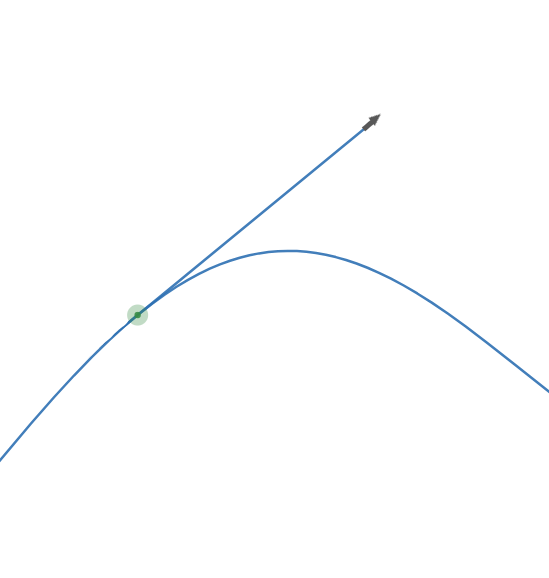
\includegraphics[width=1\textwidth]{image/derivata3}
\caption{Raffigurato il vettore velocità $\vec{v}$}
\label{img:derivata}
\end{minipage}%
\hspace{10mm}%
\begin{minipage}[c]{0.45\textwidth}
\centering
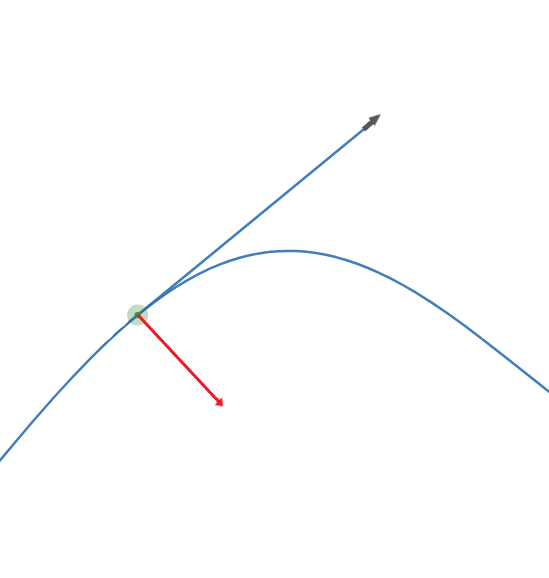
\includegraphics[width=1\textwidth]{image/accelerazione}
\caption{Raffigurato il vettore accelerazione in rosso $\vec{a}$}
\label{img:accelerazione}
\end{minipage}
\end{figure}


\subsection{Cinematica Unidimensionale}

\paragraph{}
La cinematica unidimensionale studia il movimento di un corpo lungo una retta fissando un'origine, chiamata O, un verso di percorrenza e un'unità di misura.

In questa parte trattiamo i due moti rettilinei:
\begin{itemize}
    \item \textit{Moto rettilineo uniforme}
    \item \textit{Moto rettilineo uniformemente accelerato}.
\end{itemize}

\paragraph{}
\subsubsection{Moto rettilineo uniforme:}
Il \textit{moto rettilineo uniforme} è caratterizzato da avere \textit{velocità costante} e \textit{accelerazione uguale a zero}.
\paragraph{}
\textbf{Legge oraria:}
\begin{equation}
    x(t) = x_0 + \vec{v}\Delta t
    \label{leggeOrariamrUnivrome}
\end{equation}

\paragraph{}
Se volessimo rappresentare sul piano cartesiano, in funzione del tempo e dello spazio, questo moto risulterebbe essere una retta nel primo quadrante.

Sull'asse delle ascisse inseriamo la variabile indipendente : $\vec{t}$, mentre sull'asse delle ordinate inseriamo lo spostamento effettuato: $x$. Figura \ref{img:motorettuniforme}.

In Figura \ref{img:TIKZmotorettuniforme} vediamo la relazione tra spazio percorso, velocità costante e accelerazione nulla. Essendo l'accelerazione di questo moto costante, immaginando di essere nello spazio, il corpo continuerebbe con una certa velocità a viaggiare nello spazio percorrendo in ogni $\Delta t$ il medesimo spazio.  
\paragraph{}

\begin{figure}[H]
\centering
\begin{minipage}[c]{0.40\textwidth}
\centering
\begin{tikzpicture}
\begin{axis}[
    axis lines = left,
    xlabel = $t$,
    ylabel = {$s$},
]
\addplot [
    domain=0:4,
    samples=100, 
    color=black,
]{x};
\end{axis}
\end{tikzpicture}
\caption{Grafico Moto Rettilineo Uniforme}
\label{img:motorettuniforme}
\end{minipage}%
\hspace{20mm}%
\begin{minipage}[c]{0.40\textwidth}
\centering
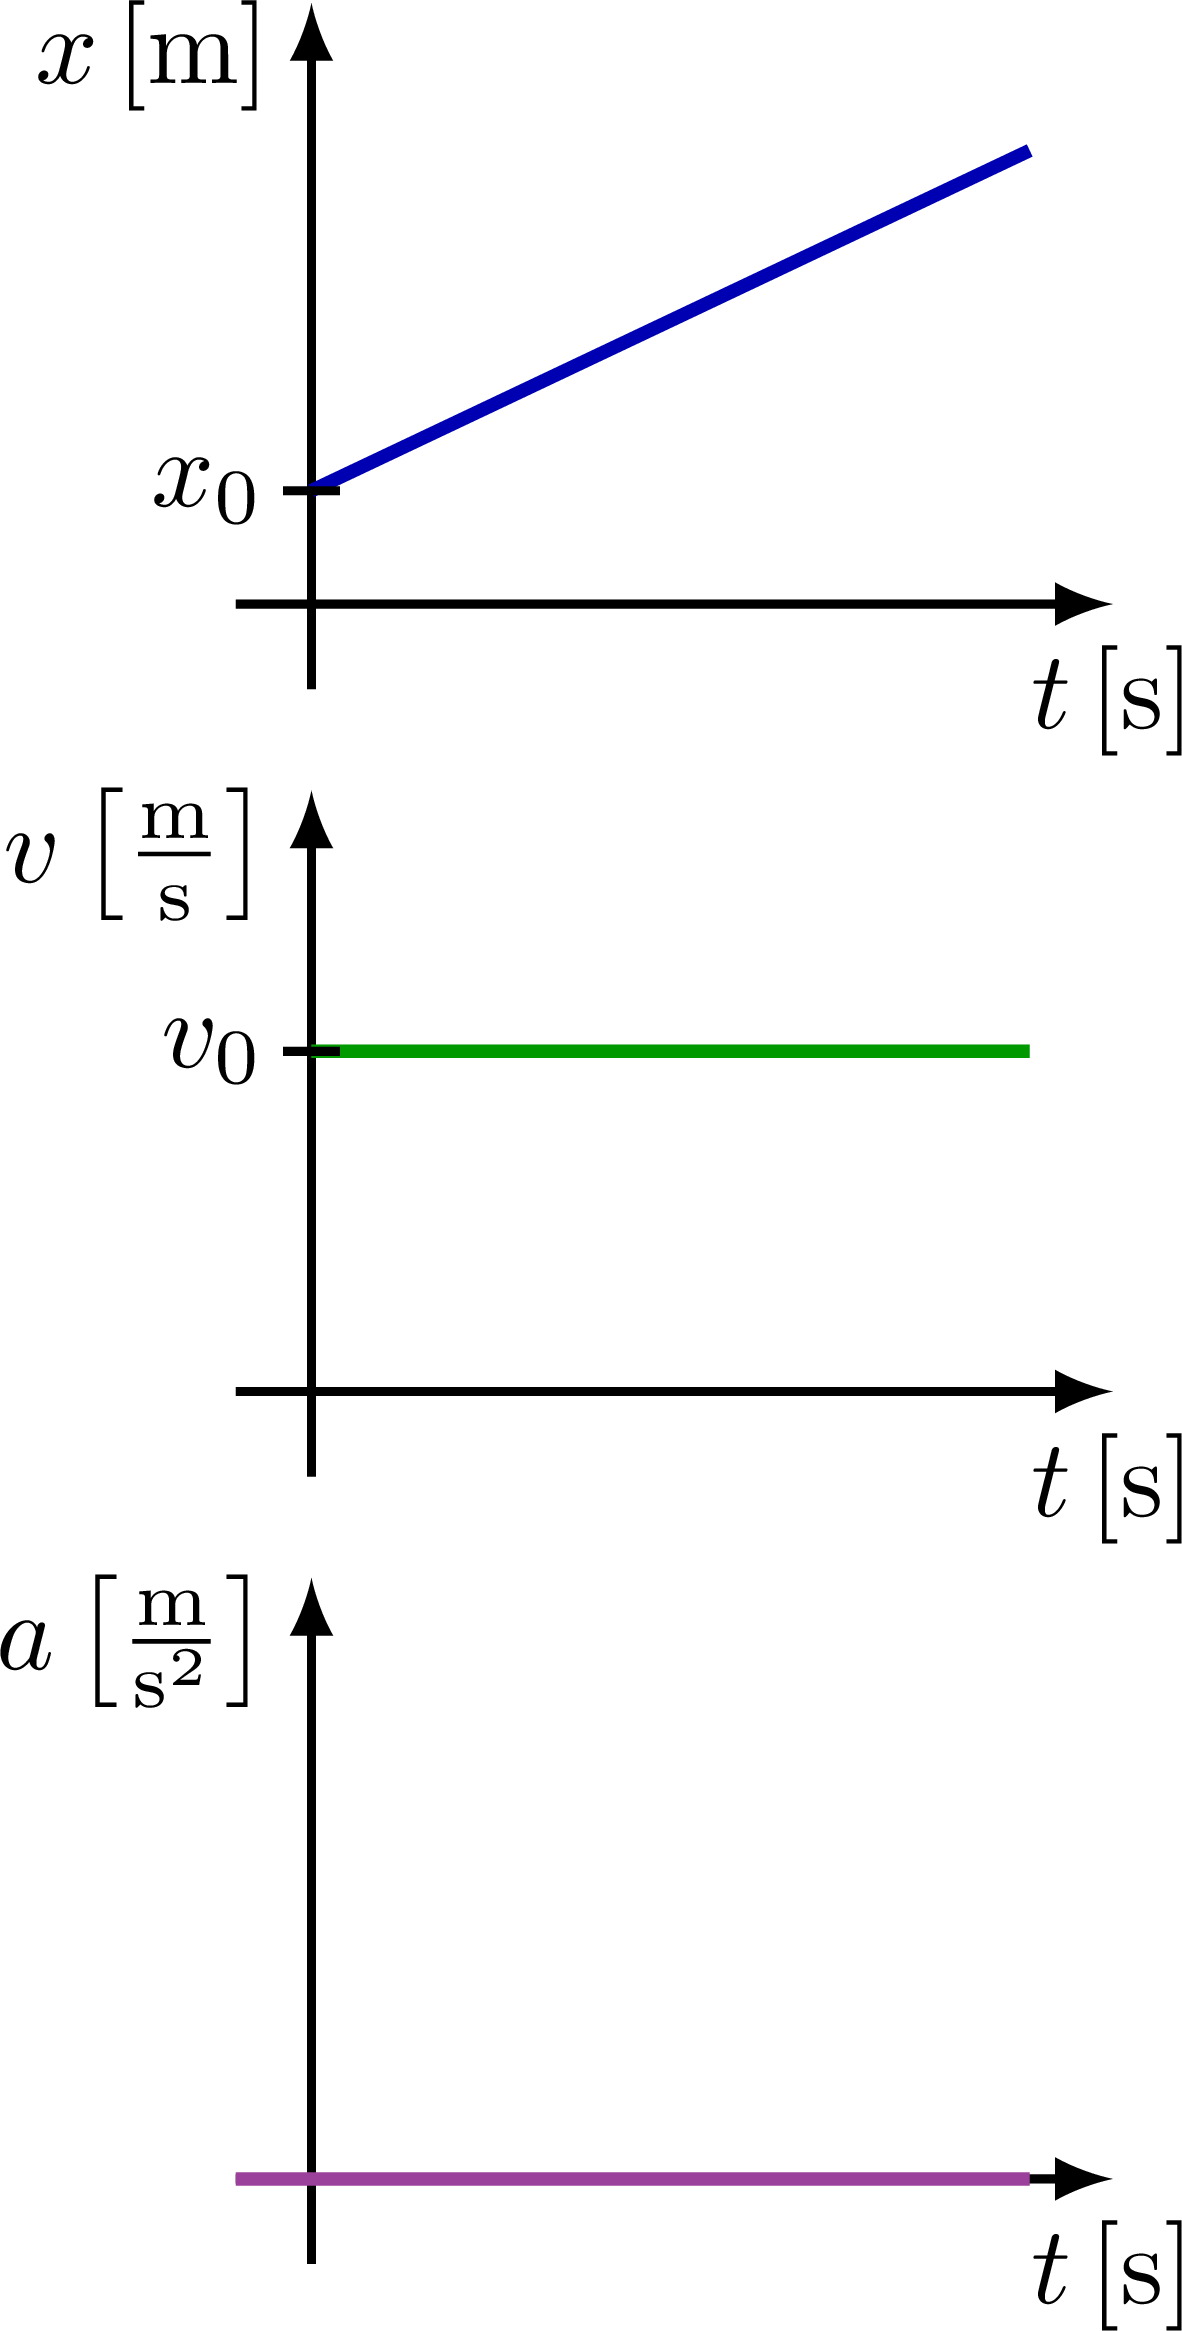
\includegraphics[width=1\textwidth]{image/motoUniforme.png}
\caption{Relazione tra spostamento, velocità e accelerazione}
\label{img:TIKZmotorettuniforme}
\end{minipage}
\end{figure}

\subsubsection{Moto rettilineo uniformemente accelerato:}Un corpo sottoposto a \textit{Moto rettilineo uniformemente accelerato} subisce sempre un'accelerazione costante: si definisce, rispetto al \textit{moto rettilineo uniforme}, un moto vario.

Avendo accelerazione costante $\vec{a}_{cost.}$ la velocità cresce o diminuisce sempre della stessa quantità, quindi in un lasso di tempo vedremo che la variazione di spazio crescerà in maniera quadratica rispetto al tempo.

\paragraph{}
\textbf{Legge oraria:}
\begin{equation}
\label{leggeOrunifacc}
    x(t) = x_0 + \vec{v}_0\Delta t+\frac{1}{2}\vec{a}\Delta t\,^2
\end{equation}
da cui derivano anche:
\begin{equation*}
    \vec{v}=\vec{v_0} + \vec{a}\Delta t \qquad{} \vec{v}\,^2 = \vec{v_0}^2 + 2\vec{a}\Delta x
\end{equation*}
\paragraph{}

Essendo questo moto accelerato costantemente, osserveremo che sul grafico ad ogni unità di tempo lo spostamento sarà sempre maggiore dettato dal fatto che la velocità continua a crescere uniformemente via via che scorre il tempo. Figura \ref{img:motorettuniformementeacc}.
La figura \ref{img:TIKZmotoUniformementeAcc} mostra un corpo che inizialmente ha velocità negativa ma ad un certo istante $t$ cambia direzione, mantenendo sempre velocità constante.


Si pensi ad un pallone lanciato verso l'alto. Inizialmente avrà una velocità data dallo sforzo compiuto dalle nostre braccia per lanciarlo in alto. Sul pallone però agisce fin da subito l'accelerazione gravitazionale la quale farà si che perderà velocità, fino a raggiungere l'altezza massima dove si fermerà, ed inizierà la sua caduta verso il centro della terra. 


\begin{figure}[H]
\centering
\begin{minipage}[c]{0.40\textwidth}
\centering
\begin{tikzpicture}
\begin{axis}[
    axis lines = left,
    xlabel = $t$,
    ylabel = {$s$},
]
\addplot [
    domain=0:4, 
    samples=100, 
    color=black,
]{0.2*x^2};
%\addlegendentry{\(x\)}
\end{axis}
\end{tikzpicture}
\caption{Moto Uniformemente Accelerato}
\label{img:motorettuniformementeacc} 
\end{minipage}%
\hspace{20mm}%
\begin{minipage}[c]{0.40\textwidth}
\centering
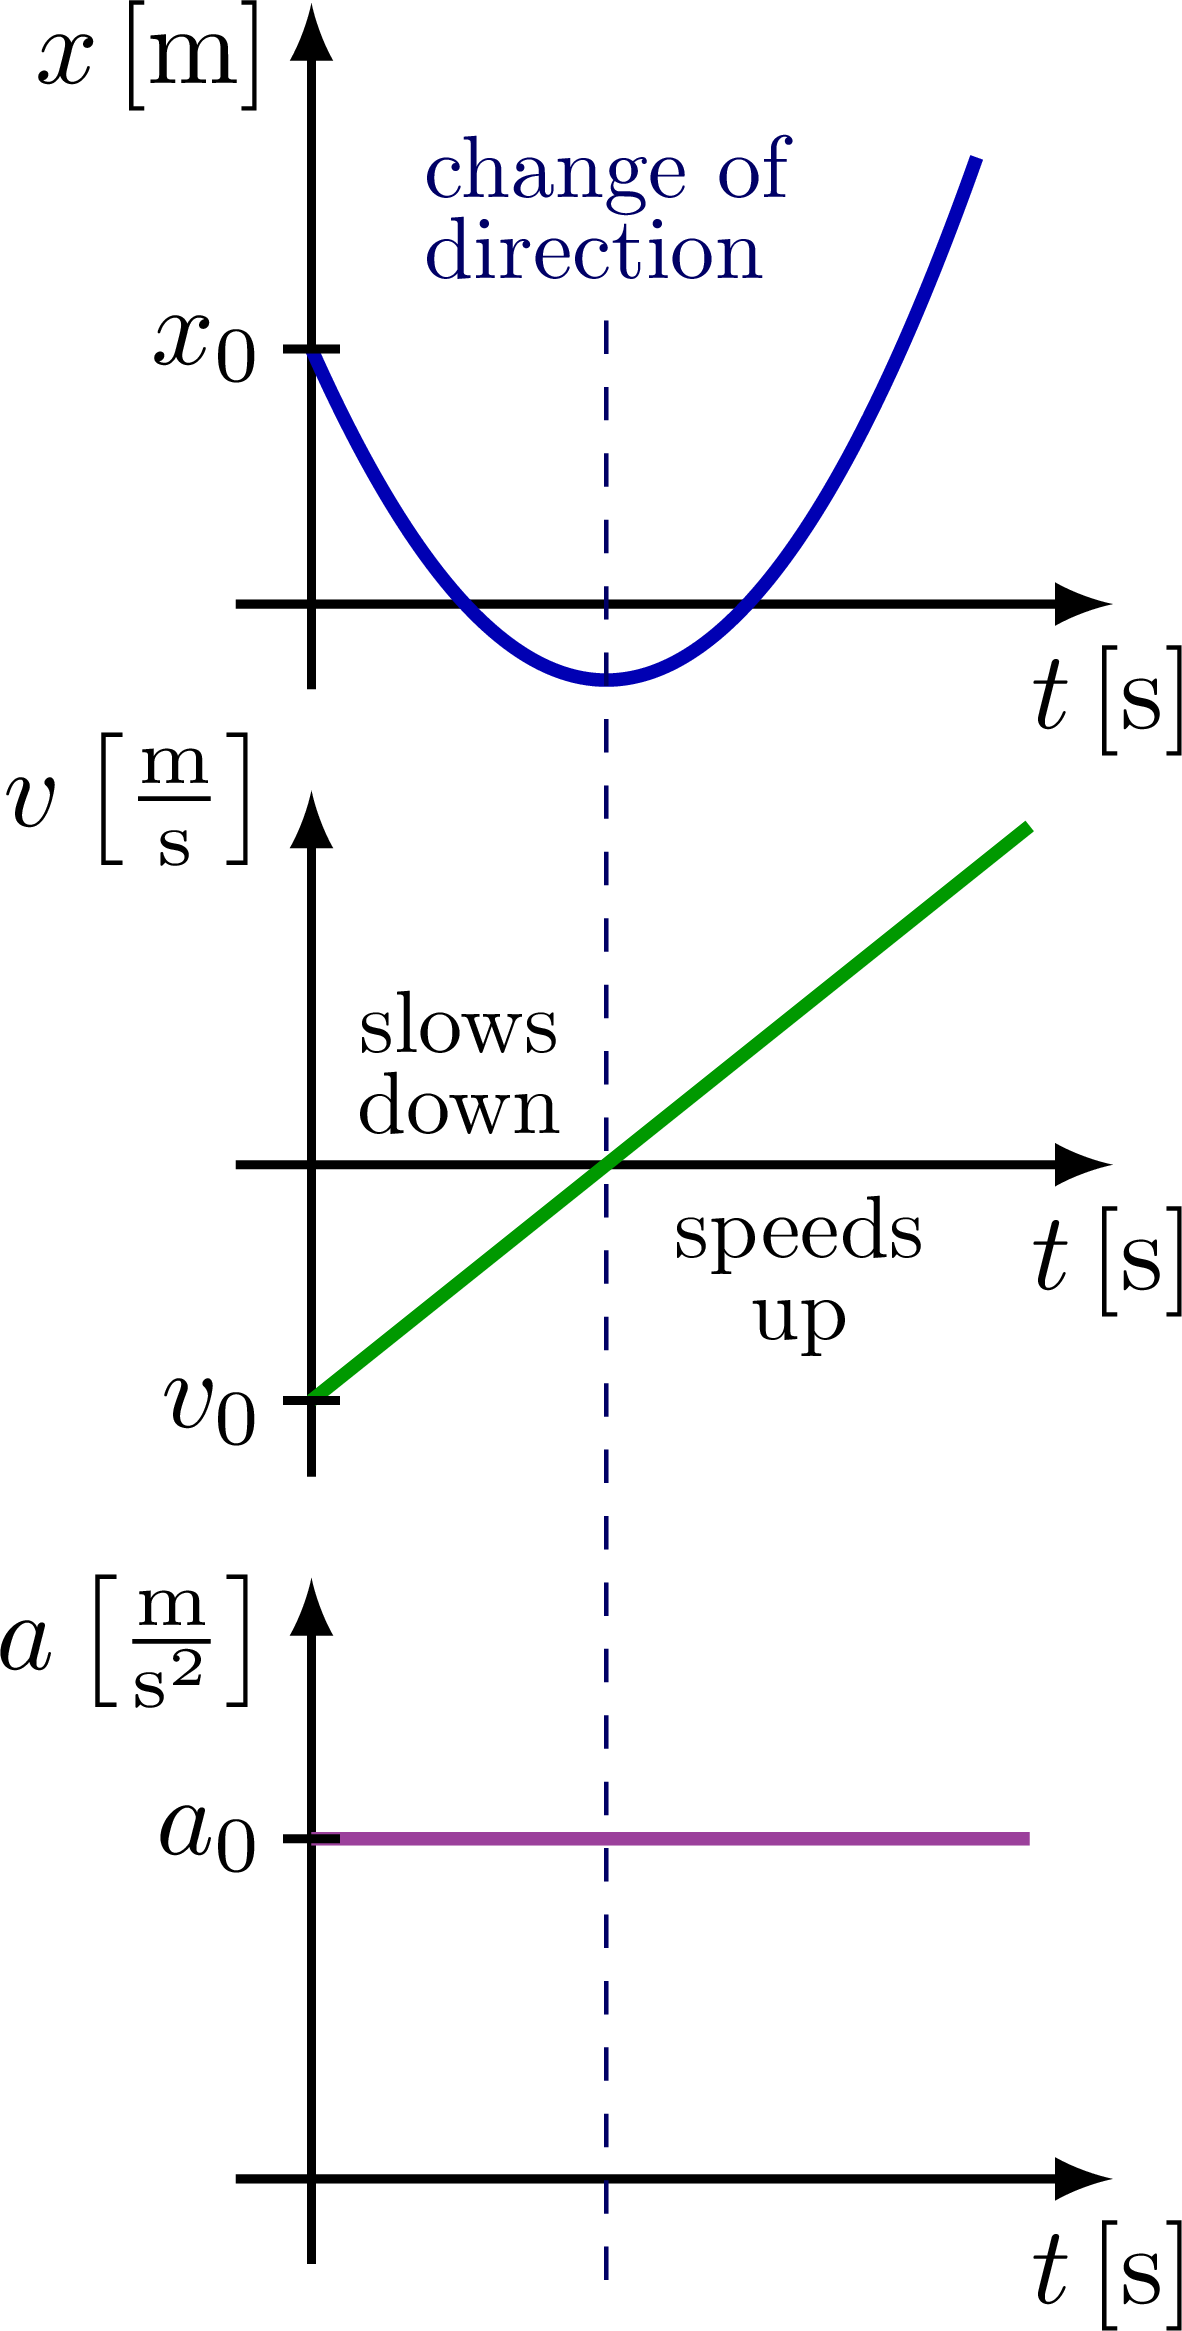
\includegraphics[width=1\textwidth]{image/motoUniformementeAcc.png}
\caption{Inversione di direzione}
\label{img:TIKZmotoUniformementeAcc}
\end{minipage}
\end{figure}

\subsection{Cinematica Multidimensionale}
Per rappresentare le coordinate in un sistema di riferimento cartesiano esistono due metodi:
\begin{itemize}
    \item coordinate cartesiane
    \item coordinate polari
\end{itemize}

\paragraph{}
In \textit{coordinate cartesiane} un punto è rappresentato come combinazione lineare di due vettori: uno posto sulle ascisse e l'altro sulle ordinate. Figura: \ref{coordinateCartesiane}.
\begin{equation*}
    \vec{r} = x\vec{i} + y\vec{j}
\end{equation*}

\paragraph{}
In \textit{coordinate polari} un punto è rappresentato da un versore ortonormale e un angolo $\theta$. Figura: \ref{img:coordPolari}.
\begin{equation*}
    \vec{r} = \vec{r}\,\vec{u}_r \quad,\quad{} dove \qquad{}\vec{u}_r  = \cos({\theta})\vec{i} + \sin({\theta})\vec{j}
\end{equation*}

\begin{figure}[tb]
\centering
\begin{minipage}[c]{0.50\textwidth}
\centering
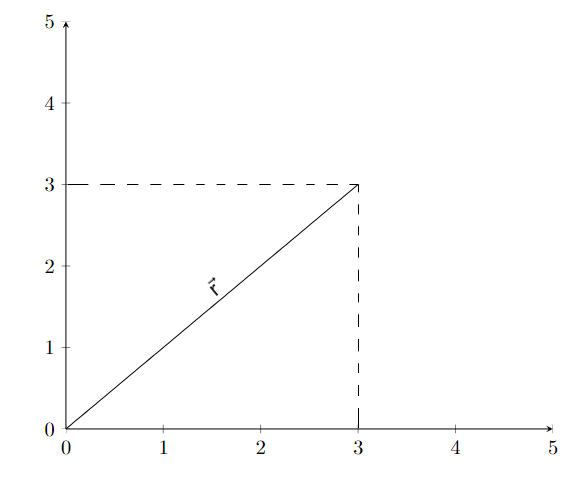
\includegraphics[width=1\textwidth]{image/ccartesiane}
\caption{Piano cartesiano}
\label{coordinateCartesiane}
\end{minipage}%
\hspace{0mm}%
\begin{minipage}[c]{0.50\textwidth}
\centering
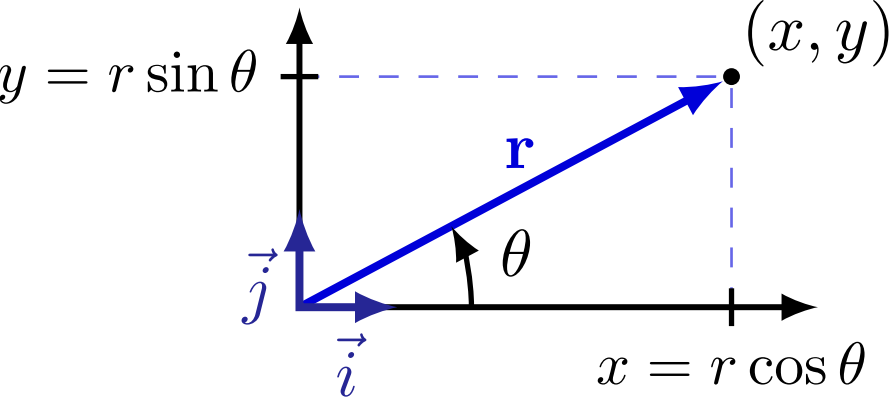
\includegraphics[width=1\textwidth]{image/coordPolari2.png}
\caption{Coordinate polari}
\label{img:coordPolari}
\end{minipage}
\end{figure}

\paragraph{}
\subsubsection{Moto parabolico:}
Il \textit{Moto parabolico} gode di due forze che agiscono sul corpo: una forza orizzontale e una forza verticale diretta verso il basso.

La componente orizzontale si muove di \textit{moto rettilineo uniforme}, la componente verticale invece si muove, verso il basso, con \textit{moto rettilineo uniformemente accelerato}, questo dovuto alla forza di gravità.

\paragraph{}
\textbf{Legge oraria:}

$$
\begin{cases}

     x(t) = x_0 + \vec{v}_x\Delta t\\
     y(t) = y_0 + \vec{v}_{y0}\Delta t-\frac{1}{2}\vec{g}\Delta t\,^2
     
\end{cases}
$$

da cui derivano anche:
\begin{equation*}
    y_{max} = \frac{\vec{v}_{y0}\,^2}{2\vec{g}}\,, \quad t_{volo} = \frac{2\vec{v}_{0y}}{\vec{g}}\,, \quad x_{max} = \frac{2\vec{v}_{0x}\vec{v}_{0y}}{\vec{g}} = \frac{2\vec{v_0}\sin(2\theta)}{g}
\end{equation*}


\begin{figure}[H]
    \centering
    \begin{minipage}[c]{0.45\textwidth}
        \centering
        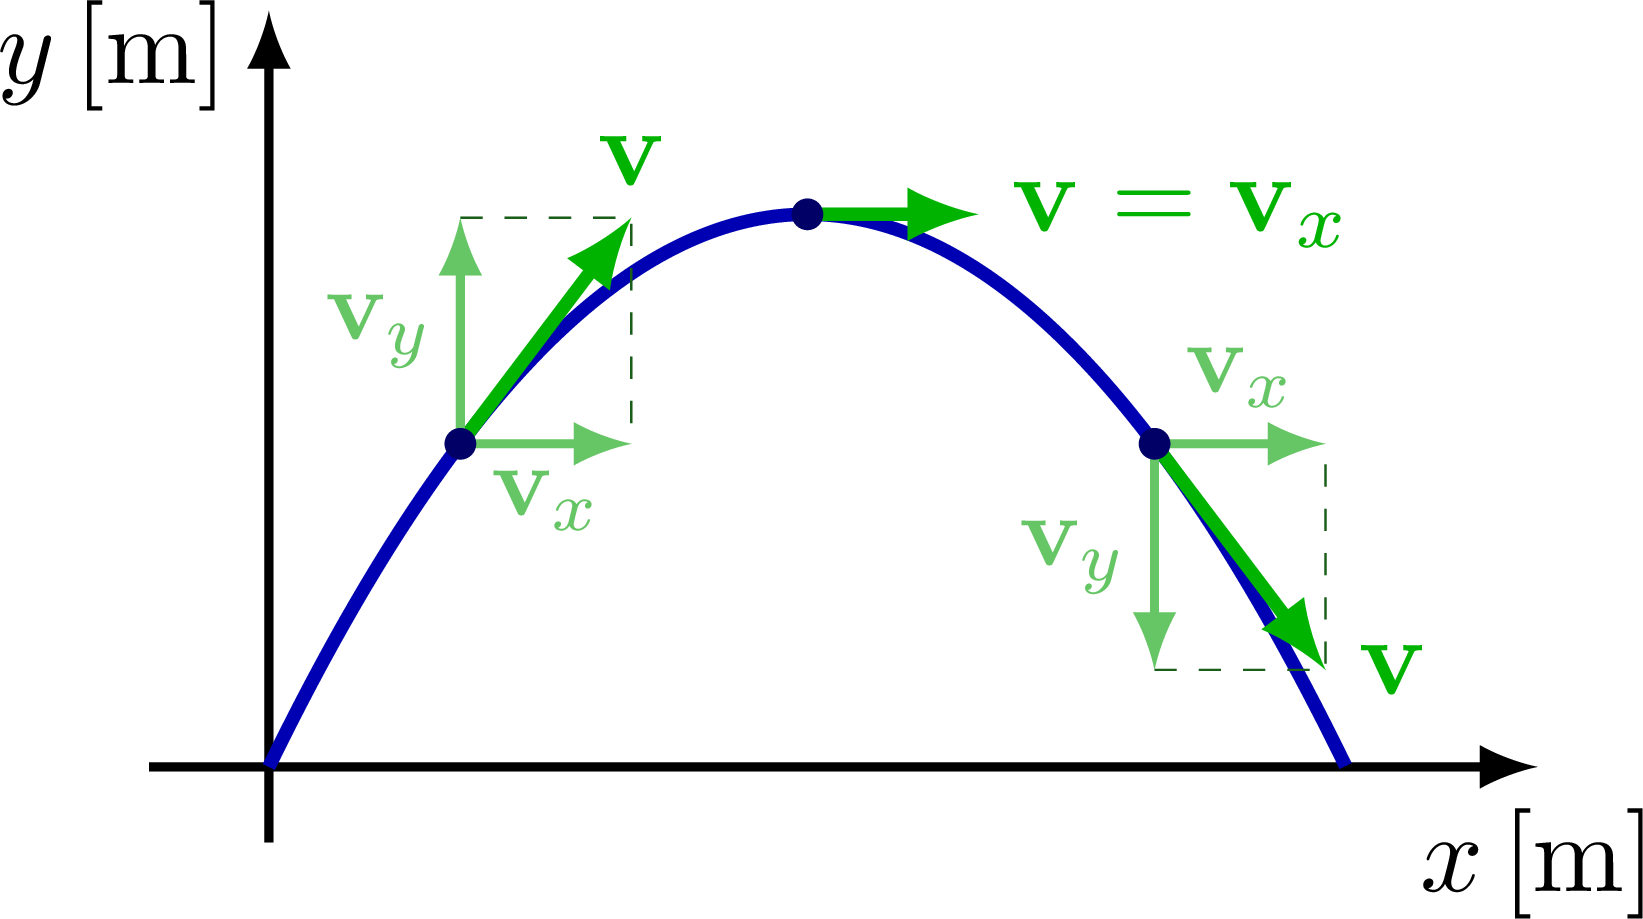
\includegraphics[width=1\textwidth]{image/motoParabolico.png}
        \caption{Moto parabolico}
        \label{fig:motoPara}
    \end{minipage}%
    \hspace{10mm}%
    \begin{minipage}[c]{0.45\textwidth}
        \centering
        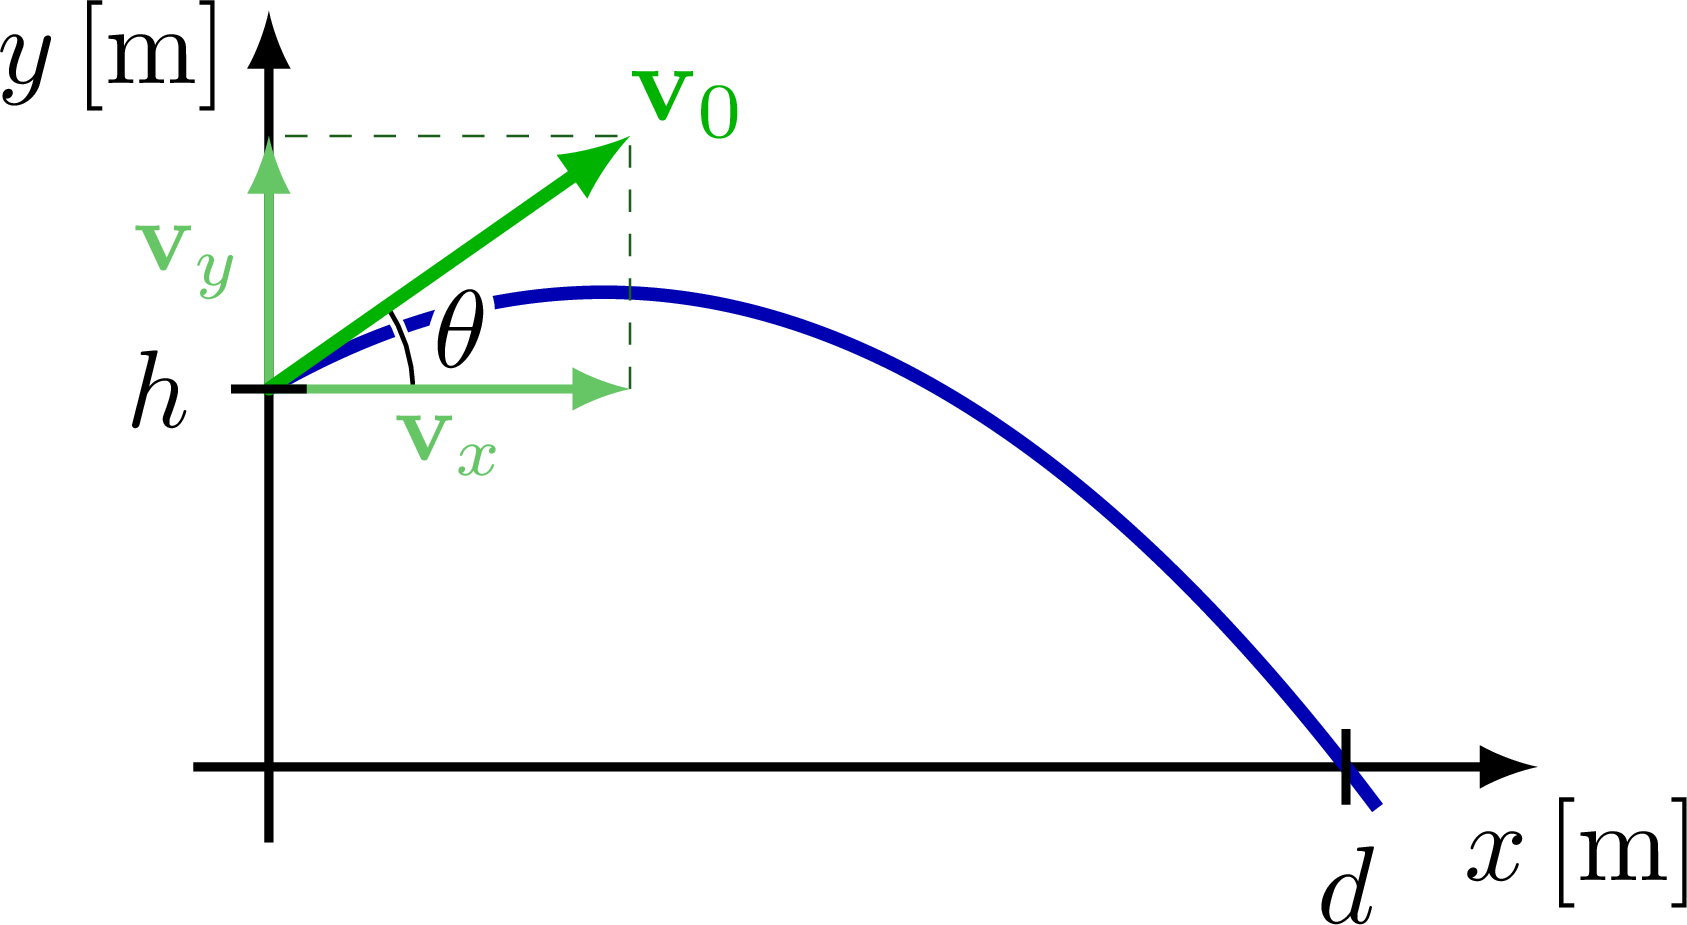
\includegraphics[width=1\textwidth]{image/motoParabolicoinAltezza.png}
        \caption{Moto parabolico da un'altezza h}
        \label{img:motoParaAltezza}
    \end{minipage}
\end{figure}


\subsection{Esercizi}

\subsubsection{Esercizio 1}
Stai guidando un'auto a 66 km/h, e stai avvicinandoti ad un semaforo. A quanti metri al secondo stai viaggiando? [sol: 18,3 $\frac{m}{s}$]

\paragraph{}
Dobbiamo trasformare i  66 km/h in m/s: 
\begin{equation*}
    66km = 66000 m\quad \text{e} \quad h = 3600 s,\quad \text{da cui}\quad \frac{66*1000}{3600} \frac{m}{s} = \frac{66}{3.6} = 18.3\frac{m}{s}
\end{equation*}
\paragraph{}
Ti stai avvicinandoti ad un semaforo. Quando arrivi a 726 m prima del semaforo, il semaforo diventa rosso, ma, un po' per la distanza, un po' per distrazione, impeghi 10.1 s per accorgertene. Appena te ne accorgi, inizi a frenare. A quale distanza ti trovi dal semaforo quando inizi a frenare? [sol: 541.17m]

\paragraph{}
Usando la formula \ref{leggeOrariamrUnivrome} troviamo la distanza percorsa in quei 10,1s di distrazione:

\begin{equation*}
    x = 18.3\frac{m}{s}*10.1s
    x = 184.83m 
    (723-184.83)m = 541.17m
\end{equation*}  

Per trovare la distanza dal semaforo sottraiamo la distanza iniziale con la distanza percorsa in 10.1s:

\begin{equation*}
    (723-184.83)m = 541.17m
\end{equation*}

\paragraph{}
Quale decelerazione devi dare per fermarti esattamente dove si trova il semaforo?[sol: 0.311$\mss$]
\paragraph{}
Usiamo le formule \ref{leggeOrunifacc}
\begin{equation*}
    0^2 = 18.3^2 + 2\vec{a}(541.17)\quad \vec{a} =\frac{(-18.3)^2}{2*541.17}= 0.311\mss
\end{equation*}

\paragraph{}
Quanto impieghi a fermarti, da quando scatta il rosso?[sol: 69,1 s]

Usiamo sempre le formule \ref{leggeOrunifacc}
\begin{equation*}
    18.3\ms=0\ms+0.311\mss*t \quad t =\frac{18.3\ms}{0.311\mss} = 59,1 s \quad (59+10.1)s = 69.1s
\end{equation*}

\paragraph{Esercizio 2}
Romeo si trova sotto il balcone di Giulietta, che è 5.3 m più in alto. Le lancia un messaggio avvolgendolo ad un piccolo sasso, ma un po' troppo forte: così, il sasso arriva più in alto di Giulietta, che non riesce a prenderlo mentre sale... ma riesce a prenderlo quando, scendendo, il sasso cade a 3.1 m/s. A che velocità ha lanciato il messaggio Romeo?

\paragraph{}
Utilizziamo le formule \ref{leggeOrariamrUnivrome} e \ref{leggeOrunifacc}. Uno schizzo del disegno potrebbe essere il seguente: \ref{img:giulietta}

\begin{figure}[tb]
\centering
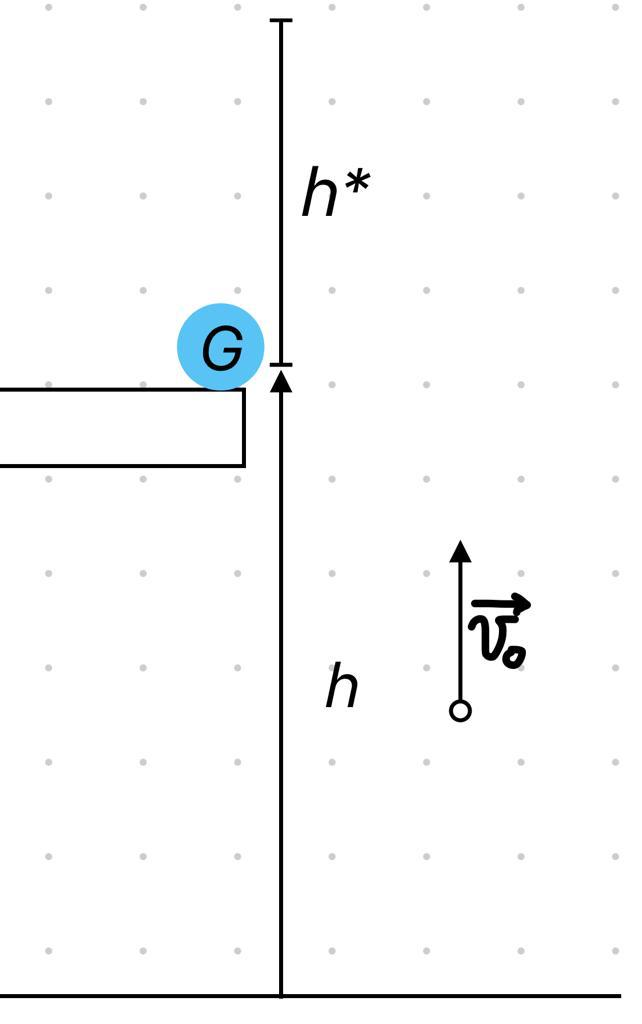
\includegraphics[width=0.30\textwidth]{image/giulietta}
\caption{Esercizio 2}
\label{img:giulietta}
\end{figure}

$$
\begin{cases}
    h + h* = \vec{v}_o - \frac{1}{2}\vec{a}t^2\\
    \vec{v}_ot - at = 0
\end{cases}
$$

Dobbiamo trovare \textit{h*}. Sappiamo che quando arriva all'altezza massima, \textit{h+h*}, la sua velocità sarà pari a zero. Quando poi ricomincia a cadere sappiamo che Giulietta lo prenderà quando il sasso ha una velocità finale di 3.1$\ms$

\begin{equation*}
    \vec{v}_f = \vec{v}_f + \vec{a}t \quad t = \frac{3.1\ms}{9.81\mss} = 0.31s
\end{equation*}

In questo laso di tempo il sasso si sposta di h*, calcoliamolo.

\begin{equation*}
    h* = \frac{1}{2}\veca t^2 = \frac{1}{2}*9.81\mss*(0.31s)^2 = 0.47m
\end{equation*}

A questo punto abbiamo trovato l'altezza massima: 

\begin{equation*}
    h + h* = 5.3+0.47 = 5.77m
\end{equation*}

e possiamo risolvere, mediamte il sistema impostato ad inizio esercizio, la velocità iniziale.

\begin{equation*}
    5.77m = \vv_0t-\frac{1}{2}\vv_0\quad{} => 
\end{equation*}
$$
\begin{cases}
    \vv_o t = 11.54m => t=\frac{11.54m}{\vv_o}\\
    \vv_o = \veca*\frac{11.54m}{\vv_o} => \vv_o\,^2 = 9.81\mss*11.54m => \vv_o = 10.64\ms
\end{cases}
$$

\paragraph{}
A quale velocità avrebbe dovuto lanciare il sasso Romeo perché arrivasse giusto giusto all'altezza di Giulietta?
\begin{equation*}
    0^2 = \vv_o ^2 + 2*9.81\mss*5.3m \quad \vv_o = \sqrt{2*9.81*5.3} = 10.20\ms
\end{equation*}

\paragraph{}
Se avvenisse sulla luna, a quale velocità avrebbe dovuto lanciare il sasso Romeo perché arrivasse giusto giusto all'altezza di Giulietta? E su giove?
\begin{equation*}
    0^2 = \vv_o ^2 + 2*(\frac{9.81}{6})\mss*5.3m \quad \vv_o = \sqrt{2*1.64*5.3} = 4.17\ms\\
\end{equation*}

\text{su giove invece...}

\begin{equation*}
    0^2 = \vv_o ^2 + 2*(\frac{24.79}{6})\mss*5.3m \quad \vv_o = \sqrt{2*24.79*5.3} = 16.21\ms
\end{equation*}


\paragraph{Esercizio 3}
Quale accelerazione deve avere un'automobile, in unità internazionali, per andare da 0 a 54.0 mph in 8.7 s?
mph significa, in inglese, "miles per hour". Un miglio anglosassone corrisponde a 1609 metri. [2.77$\mss$]

Svlogimento.

54mph = 54*1.609 = 86.87km/h = 24.13m/s

\begin{equation*}
    24.13\ms = \veca*8.7s \qquad{} \veca = \frac{24.13\ms}{8.7s} = 2.77\mss
\end{equation*}

Quale frazione di g è questa accelerazione?
\begin{equation*}
    9.81:100 = 2.33:x\qquad{} x = 28\%
\end{equation*}

Quale distanza ha percorso l'automobile , in piedi anglosassoni?[3.28m ]
Un piede anglosassone ("foot") corrisponde a 30,48 cm, e si apprevia con "ft".
\begin{equation*}
    x = \frac{1}{2}*2.77\mss(8.7s)^2 = 104.83m \quad{} 1ft = \frac{1}{0.3048} = 3.28m 
\end{equation*}
\begin{equation*}
    104.84*\frac{1}{0.3048} = 343.96ft
\end{equation*}

Se dovesse frenare decelerando della metà dell'accelerazione iniziale, quanto spazio occorrerebbe per fermarsi?[209.44m]

\begin{equation*}
    \veca = \frac{2.72}{2} = 1.39\mss \quad 0 = 24.13\ms + 1.39\mss t
\end{equation*}
\begin{equation*}
    t = \frac{24.13\ms}{1.39\mss} = 17.36s\quad x = \frac{1}{2}*1.39\mss*(17.36s)^2 = 209.44m
\end{equation*}

\paragraph{Esercizio 4}
Una nuotatrice riesce ad andare a 0,4 m/s quando è in acqua ferma. Sta attraversando  un fiume largo 34 m, con una corrente che scorre a 0,21 m/s. La nuotatrice punta perpendicolarmente all'altra riva.
A quale distanza a valle, rispetto alla perpendicolare, approda all'altra riva?[17.85m] 

Quanto tempo impiega ad attraversare il fiume?[85s]

Con quale angolo dovrebbe dirigersi a monte, rispetto alla perpendicolare alla riva, per attraversare effettivamente il fiume perpendicolarmente alla riva?[32°] 

Quanto ci metterebbe in questo caso ad attraversare il fiume?[96s]
\begin{figure}[tb]
\centering
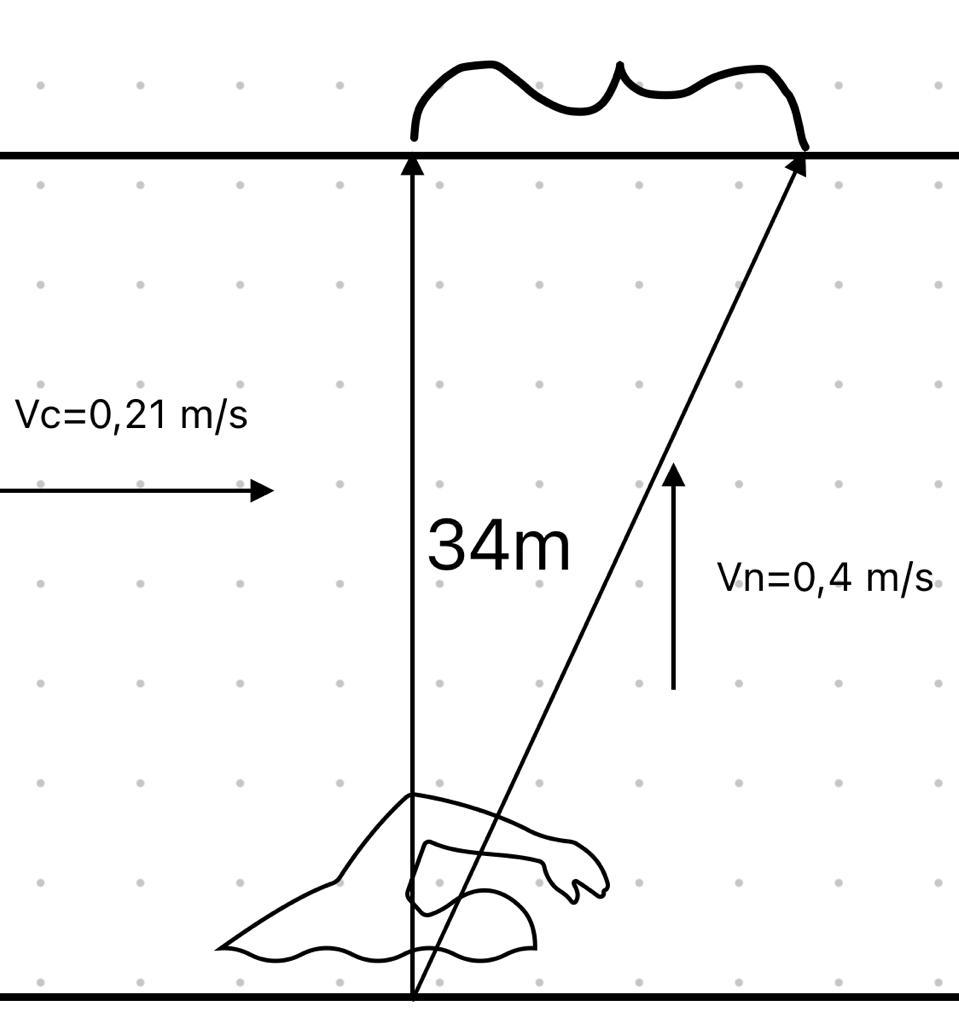
\includegraphics[width=0.45\textwidth]{image/nuotatrice}
\caption{Esercizio 4}
\label{img:nuotatrice}
\end{figure}

\paragraph{Svolgimento:}
 

calcoliamo quanto tempo impiega per attraversare la sponda...
\begin{equation*}
    34m = 0.4\ms t\qquad{} t = \frac{34n}{0.4\ms} = 85s
\end{equation*}
calcoliamo di quanti metri ha spostato la nuotatrice la corrente
\begin{equation*}
    x = 85s*0.21\ms = 17.85m
\end{equation*}

Siccome la nuotatrice mantiene sempre la stessa velocità anche rivolta verso monte allora l'angolo deve essere: 
\begin{equation*}
    0.4\ms \sin{\alpha} = 0.21\ms \qquad{} \arcsin{\alpha} = \frac{0.21}{0.4}\ms = 32\gradi
\end{equation*}

Per rispondere all'ultima domanda troviamo l'ipotenusa del triangolo in figura \ref{img:nuotatrice}:

\begin{equation*}
    ip = \sqrt{17.85^2 + 34^2} = 38.40m\,;\qquad{} 38.40m = 0.4\ms t
\end{equation*}
\begin{equation*}
    t = \frac{38.40m}{0.4\ms} = 96s
\end{equation*}

\paragraph{Esercizio 5}
Un atleta di salto in lungo lascia il suolo con un angolo di lancio di $45\gradi$ rispetto all’orizzontale e atterra a una distanza di 8m. Qual è la velocità di decollo $V_0$ ? 

Adesso sta facendo una corsetta all’aria aperta e giunge sulla riva sinistra di un piccolo fiume. Non c’è un ponte in vista e la riva a destra dista 10 m in orizzontale e 2,5 m in verticale verso il basso. Se l’atleta salta dal ciglio della riva sinistra con un angolo di $45\gradi$ con la velocità calcolata nel punto precedente, quanto dopo o quanto prima atterrerà rispetto alla riva opposta?

\begin{figure}[tb]
\centering
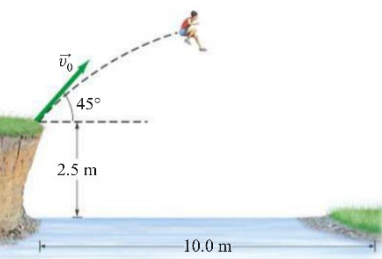
\includegraphics[width=0.45\textwidth]{image/salto}
\caption{Esercizio 5}
\label{img:salto}
\end{figure}




\paragraph{Svolgimento:}

Utilizzando il la legge oraria del moto parabolico avremo che:

$$
\begin{cases}

     x = \vec{v}_0\cos{\theta}t\\
     y = \vec{v}_0\sin{\theta}t-\frac{\vec{g}}{2}t\,^2
     
\end{cases}
$$

ci interessa $V_0$ a noi, troviamo il tempo.

\begin{equation*}
    t=\frac{x}{V_0\cos{\theta}}
\end{equation*}

sostituiamo nella seconda equazione ed otteniamo:


\begin{equation*}
    0 = \frac{xV_0\sin{\theta}}{V_0\cos{\theta}}-\frac{g}{2}\frac{x^2}{(V_0\cos{\theta})^2}
\end{equation*}
\begin{equation*}
    V_0 = \sqrt{\frac{gx}{\sin{2\theta}}} = \sqrt{\frac{9.81*8.0}{\sin{2*45}}} = 8.86\ms
\end{equation*}

Rispondiamo al secondo quesito: 

Osserviamo che ora la distanza del fiume è 10m, sapendo che salta con una  $V_0$ pari a $8.86\ms$ ce la farà o no a raggiungere l'altra sponda?
Siccome nella seconda equazione abbaimo solo il tempo come incognita troviamo il tempo e successivamente sostituiamo nella prima per capire se l'atleta finirà in acqua o si salva da un bel tuffo freddo!


\begin{equation*}
    t = \frac{V_0\sin{\theta}}{g}\Biggl(1+\sqrt{1+\frac{2hg}{V_0^2(\sin{\theta})^2}}\Biggl)
\end{equation*}

sostitendo nella prima\dots


\begin{equation*}
    x = \frac{V_0^2\st\ct}{g}\Biggr(1+\sqrt{1+\frac{2hg}{V_0^2(\st)^2}}\Biggl) = \frac{V_0^2\sin{2\theta}}{2g}\Biggr(1+\sqrt{1+\frac{2hg}{V_0^2(\st)^2}}\Biggl)
\end{equation*}
\begin{equation*}
    x = \frac{8.86^2*1}{2*9.81}\Biggr(1+\sqrt{1+\frac{2*2.5*9.81}{8.86^2*0.5}}\Biggl)= 10m
\end{equation*}

A pelo!

%   MAGARI INSERIRE ALTRI ESERCIZI % 

\newpage
\section{Leggi di Newton}
I $3$ principi della dinamica, o \textit{leggi di Newton}, sono le leggi classiche fondamentali per la descrizione del moto.

\paragraph{}
Il \textbf{\textit{principio di inerzia}} afferma che:

Un corpo in un sistema di riferimento inerziale (senza sollecitazioni) o è in \textit{quiete}, se non è sottoposto ad alcuna forza o le forze risultanti sono nulle, o gode di un moto di tipo \textit{rettilineo uniforme}, quindi con velocità costante e accelerazione uguale a zero.

\paragraph{}
Il \textbf{\textit{secondo principio}} afferma che:

Le cause dei moti (accelerazioni) sono dei vettori direttamente proporzionali alla forza risultante agente sull'oggetto e inversamente proporzionale alla sua massa.
\begin{equation}
    \vec{F} = m\vec{a}
    \label{secondaLeggeNewton}
\end{equation}

\paragraph{}
Il \textbf{\textit{terzo principio}}, o \textit{principio azione reazione}, afferma che:

Ogni qualvolta un corpo $A$ esercitata una forza sul corpo $B$, allora $B$ esercita una forza uguale di modulo e contraria su $A$. È intrinsecamente in ogni oggetto che possiede massa e non cambia in base alla gravità a cui è sottoposto.
\begin{equation}
    \vec{F}_{AB} = -\vec{F}_{BA}
    \label{terzaLeggeNewton}
\end{equation}

Altre leggi\dots
\paragraph{}

\textbf{\textit{Omogeneità del tempo}}: gli esperimenti non dipendono dal tempo, se tutti i fattori rimangono inalterati allora l’esperimento deve valere indistintamente dal tempo.


\textbf{\textit{Omogeneità dello spazio}}: gli esperimenti non dipendono dallo spazio o dal luogo geografico, se tutti i fattori rimangono inalterati l’esperimento rimane costante. 

\textbf{\textit{Esotropia dello spazio}}: ambiente in cui non ci sono direzioni privilegiate ad esempio si pensi ad un proiettile che viene sparato con un angolo di $45\gradi$ rispetto a Nord cade dopo tot metri, come lo stesso proiettile, a parità di condizioni iniziali, se venisse sparato verso sud.

\paragraph{}

\textbf{N.B} Secondo Newton spazio e tempo sono \textbf{assoluti}. Ora non è più vera questa affermazione in quanto nel 1905 con la teoria della \textbf{relatività ristretta}, lo spazio-tempo \textbf{dipende dall'osservatore}. La distanza spaziale o temporale risulta diversa se l'osservatore che la misura sia in moto o fermo rispetto all'oggetto osservato.

\newpage
\paragraph{Nomenclatura:}
\paragraph{}
\textit{Inerzia:} tendenza di un corpo ad opporre resistenza ad un cambio di moto. La massa, M, è la misura dell’inerzia di un corpo.

\textit{Peso:} dovuto alla forza gravitazionale che agisce su un corpo ed è uguale al prodotto della massa per l’accelerazione di gravità 

\begin{equation*}
    \vec{F} = m\veca
\end{equation*}

\textit{Forza:} vettore considerato come spinta o trazione e dato il secondo principio di Newton una forza può produrre un accelerazione. 

\textit{Forza risultante:} somma di tutte le forze agenti su un oggetto 


Il \textit{sistema di riferimento inerziale} è caratterizzato dalle seguenti condizioni: se un corpo non è sottoposto a forze o la somma delle forze risultanti è zero allora esso preserva lo stato di quiete o di moto rettilineo uniforme finché non viene perturbato. In altre parole si dice inerziale perché \textbf{l’accelerazione è pari a zero} per immaginarselo si pensi ad un oggetto nello spazio. 
Per molti esperimenti, soprattutto per quelli di breve durata, la terra può essere considerata approssimativamente un sistema di riferimento inerziale. 

\paragraph{Tipi di forze} 
\paragraph{}
\begin{align*}
\begin{tabular}{ l c r }
\toprule
Forza       &    \qquad    &   Tipo\\
\midrule
Attraente   &       \qquad    &   a distanza\\
Peso        &       \qquad    &   a distanza\\
Centripeta   &      \qquad     &   a distanza\\
Elettrica        &       \qquad    &   a distanza\\
Magnetica        &       \qquad    &   a distanza\\
Attrito        &       \qquad    &   a contatto\\
Galleggiamento &       \qquad    &   a contatto\\
Elastica &       \qquad    &   a contatto\\
\bottomrule
\end{tabular}
\end{align*}

\newpage
\subsection{Attrito}
Forza che si oppone al movimento o scorrimento di un un corpo su un'altro. Può essere di due tipi: \textit{statico} ($\mu_s$) se i due corpi sono fermi e uno o entrambi iniziano un movimento; \textit{dinamico} ($\mu_d$) se i due corpi sono già in movimento tra loro.

Normalmente
\begin{equation*}
  \mu_s > \mu_d
\end{equation*}

\subsection{Il piano inclnato}

\begin{figure}[H]
\centering
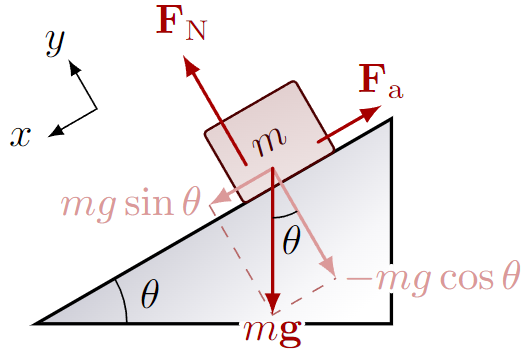
\includegraphics[width=0.45\textwidth]{image/attrito3.png}
\caption{Piano inclinato}
\label{img:pianoIncl}
\end{figure}


Il piano inclinato, un classico esempio per introdurre la scomposizione delle forza e l'attrito.

Come si vede nella Figura \ref{img:pianoIncl} stabiliamo innanzitutto un sistema di riferimento cartesiano lungo il piano inclinato. La forza peso, indicata con $ mg = \vec{F_p}$ è diretta verso il centro della terra, essa viene scomposta in due forze: una forza ortogonale al piano, indicata con $-mg\cos\theta = \vec{F_{py}}$, e una forza parallela al piano su cui poggia, indicata con $mg\sin\theta = \vec{F_{px}}$.

Per contrastare la forza peso ortogonale al piano troviamo la forza normale o reazione vincolare, indicata come $\vec{F_N} = \vec{R_V}$, che è  in direzione, verso e modulo opposto rispetto a $\vec{F_{py}}$. Se non ci fosse questa forza l'oggetto sprofonderebbe oppure sfonderebbe il sostegno sotto di esso. 

Si pensi ad un elefante su un tavolo da cucina, viene immediato a pensare che il povero tavolo venga sfondato dal pensate elefante. Infatti in questo esempio la reazione vincolare non è sufficiente per "sconfiggere" il peso dell'animale e dunque sorreggerlo.

L'ultima forza che rimane da analizzare è la forza di attrito statico, rivolta in verso e direzione opposta rispetto a $\vec{F_{px}}$ e rappresentata in figura \ref{img:pianoIncl} dalla forza $\vec{F_a}$.

\paragraph{Come trovare tutte le forze descritte in figura?}

Per il $2\gradi$ principio di Newton $(\vec{F} = m\vec{a})$ la forza peso è: 
\begin{equation*}
    \vec{F_p} = m\vec{g}\quad\bigg[\frac{N}{m}\bigg]
\end{equation*}
Dove m è la massa [Kg] dell'oggetto e $\vec{g}$ è la forza di gravità $\approx 9.81\mss$
\begin{equation*}
    \vec{F_{px}} = m\vec{g}\sin{\alpha}\quad \vec{F_{py}} = m\vec{g}\cos{\alpha}
\end{equation*}
\begin{equation*}
    \vec{F_a} = -\mu_s m\vec{g}\cos{\alpha}\quad \vec{R_v} = -m\vec{g}\sin{\alpha}
\end{equation*}



\subsection{La molla}
Una molla è un corpo capace di deformarsi a seconda delle forze che agiscono su di essa. Essa a seguito della deformazione genera una \textit{forza elastica}, che si oppone all'elongazione \footnote{Distanza rispetto alla sua posizione di equilibrio.} della molla che la induce a riacquisire la lunghezza originale.

Come si nota dalla figura \ref{img:molla} questa forza è direttamente proporzionale all'elongazione, e si esprime grazie alla legge sperimentale di Hooke, secondo la formula:

\begin{equation}
    \vec{F_e}  = -kx \qquad{con }\qquad x = L-L_0
    \label{ForzaElastica}
\end{equation}
%\clearpage  %newpage
Il segno meno nella legge di Hooke significa che la forza viene applicata in verso opposto all'elongazione: per gli allungamenti la forza di richiamo è negativa, mentre per le compressioni essa sarà positiva.

Altre formule:

\begin{itemize}
    \item costante elastica di molle in serie: $K_0 = \frac{k_1 +\dots{}+k_n}{k_1\cdot...\cdot K_n }$
    \item costante elastica di molle in parallelo: $K_0 = K_1+...+K_n$
    \item energia potenziale molla: $E_p = \frac{1}{2}K(\Delta x)^2$
    \item energia cinetica molla: $E_c = \frac{1}{2}m(\Delta v)^2$
\end{itemize}

\begin{figure}[H]%htbp H
\centering
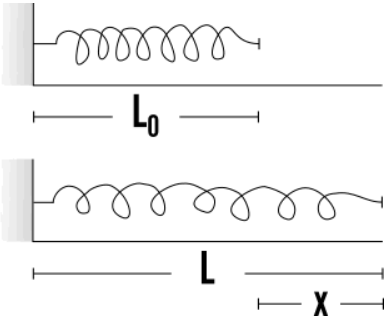
\includegraphics[width=0.45\textwidth]{image/molla}
\caption[Rappresentazio molla]{Rappresentazione elongazione molla}
\label{img:molla}
\end{figure}




\subsection{La Macchina di Atwood}

\begin{figure}[H]
    \centering
    \begin{tikzpicture}[scale=0.65]
    \centering
    % Mass 1
    \draw[thick] (1.49cm,0) -- ++(0,-5cm) node[draw=black,above=0.18cm,circle,fill=brown!70!black](cM){}
    node[draw=black,trapezium,rounded corners=1pt,fill=brown!70!black,text=white, minimum height=0.7cm](M){M};
    
    % Mass 2
    \draw[thick] (-1.49cm,0) -- ++(0,-3.5cm) node[draw=black,above=0.13cm,circle,fill=brown!70!black](cm){} node[draw=black,trapezium,rounded corners=1pt,fill=brown!70!black,text=white, minimum height=0.6cm](m){m};
    
    % Supporting structure
    \fill[pattern= north west lines,] (-2.5,2.41) rectangle (2.5,2.6);
    \draw(-2.5,2.41) -- (2.5,2.41);
    
    % Pulley
    \draw[fill = gray] (0,0) circle (1.5cm); % Big circle
    \draw[fill=lightgray] (0,0) circle (1.3cm); % Medium circle
    \draw[fill=white] (75:2.5) to[rounded corners=0.2cm] (0.2,-0.25) to[rounded corners=0.2cm] (-0.2,-0.25) -- (105:2.5) -- cycle;
    \draw[fill=darkgray] (0,0) circle (0.12cm); % Axle circle
    
    % Forces
    \draw [-latex,very thick,blue] (M.bottom side) -- ++(0,-1) node[midway,right]{$F_1$};
    \draw [-latex,very thick,black] (cM.north) -- ++(0,1)node[midway,right]{$T_1$};
    
    \draw [-latex,very thick,red] (m.bottom side) -- ++(0,-1)node[midway,left]{$F_2$};
    \draw [-latex,very thick,black] (cm.north) -- ++(0,1)node[midway,left]{$T_2$};
    
    \end{tikzpicture}
    \caption{Macchina di Atwood}
    \label{fig:atwood}
\end{figure}

La \textit{Macchina di Atwood}, raffigurata nella Figura \ref{fig:atwood}, è un apparato sperimentale ideato dal matematico inglese George Atwood per misurare l’accelerazione di gravità più facilmente e con una maggior grado di precisione di quanto non si potesse fare con il piano inclinato.

Intuitivamente si capisce che il corpo più pesante scenderà e farà ruotare la carrucola sollevando così il corpo più leggero.\\
In questo caso, per facilitare i calcoli, supponiamo che la corda e la carrucola non abbiano massa in modo tale che venga trasmessa tutta la forza senza dispersioni.

\newpage
\paragraph{}
Il concetto chiave da tenere in mente è che dovremo applicare il \textit{Secondo principio della Dinamica}: 

\begin{equation*}
    \vec{F}=m\veca
\end{equation*}

\paragraph{}

Per risolvere questi tipi di esercizi è fondamentale disegnare il \textit{Diagramma di corpo libero} già presente nell'immagine \ref{fig:atwood}, il quale rappresenta tutte le forze in gioco in un corpo massivo come ad esempio la forza peso, la tensione, la reazione vincolare, la forza di attrito\dots

Per ciascuno dei due corpi scriviamo l'equazione delle forze dettate dal \textit{Secondo principio della Dinamica}: 

$$
\begin{cases}

    M\vec{g} + T_1 = M\veca\\
    m\vec{g} + T_2 = m\veca
     
\end{cases}
$$
\begin{center}
 Dove: \qquad $M\vec{g} = F_1$ \quad ,  \quad $m\vec{g} = F_2$   
\end{center}

Poiché in entrambi i casi stiamo lavorando lungo un’unica direzione, possiamo riscrivere le precedenti equazioni specificando i segni delle grandezze coinvolte. Per il corpo M consideriamo un riferimento con verso delle coordinate crescenti rivolto verso il basso, per assecondare la forza di gravità. Per il corpo m invece prendiamo come verso delle coordinate crescenti quello rivolto verso l’alto in modo da assecondare la tensione della fune.

$$
\begin{cases}

    M\vec{g} - T_1 = M\veca\\
    -m\vec{g} + T_2 = m\veca
     
\end{cases}
$$
\begin{center}
 Dove: \qquad $M\vec{g} = F_1$ \quad ,  \quad $-m\vec{g} = F_2$   
\end{center}

Svolgendo i conti: 

\begin{equation*}
    M_1\vec{g} - mg\vec{g} = M\veca + m\veca \qquad \text{($T_1$ e $T_2$ si elidono)}
\end{equation*}

L'accelerazione di entrambi i corpi è:

\begin{equation}
    a = \frac{M-m}{M+m}\vec{g}
\end{equation}

La tensione della corda è:
\begin{equation}
    T = \frac{2 M m}{M+m}\vec{g}
\end{equation}


\newpage
\section{Moto Circolare}
Un corpo si dice che è in \textit{moto circolare} se esso si muove lungo una circonferenza di raggio $r$.

\paragraph{}
\textbf{Posizione angolare:}\\
Per descrivere questo moto conviene introdurre uno nuova grandezza fisica: \textit{la posizione angolare}. Figura \ref{fig:posizAng} \\
La \textit{posizione angolare} di un punto materiale è definita come l’angolo $\theta$ formato dal raggio passante per il punto con l’asse $x$.
La misura in radianti di un angolo $\theta$ è il rapporto fra la lunghezza l dell'arco tra l'asse $x$ e il punto e il raggio della circonferenza:

\begin{equation*}
    \theta_{rad} = \frac{l}{r} \qquad l=r\theta_{rad} \qquad 1\,rad = \frac{360\gradi}{2\pi}
\end{equation*} 

Nel SI, la posizione angolare, si misura in radianti al secondo: $\bigl[\frac{Rad}{s}\bigl]$

\begin{figure}[tb]
    \centering
    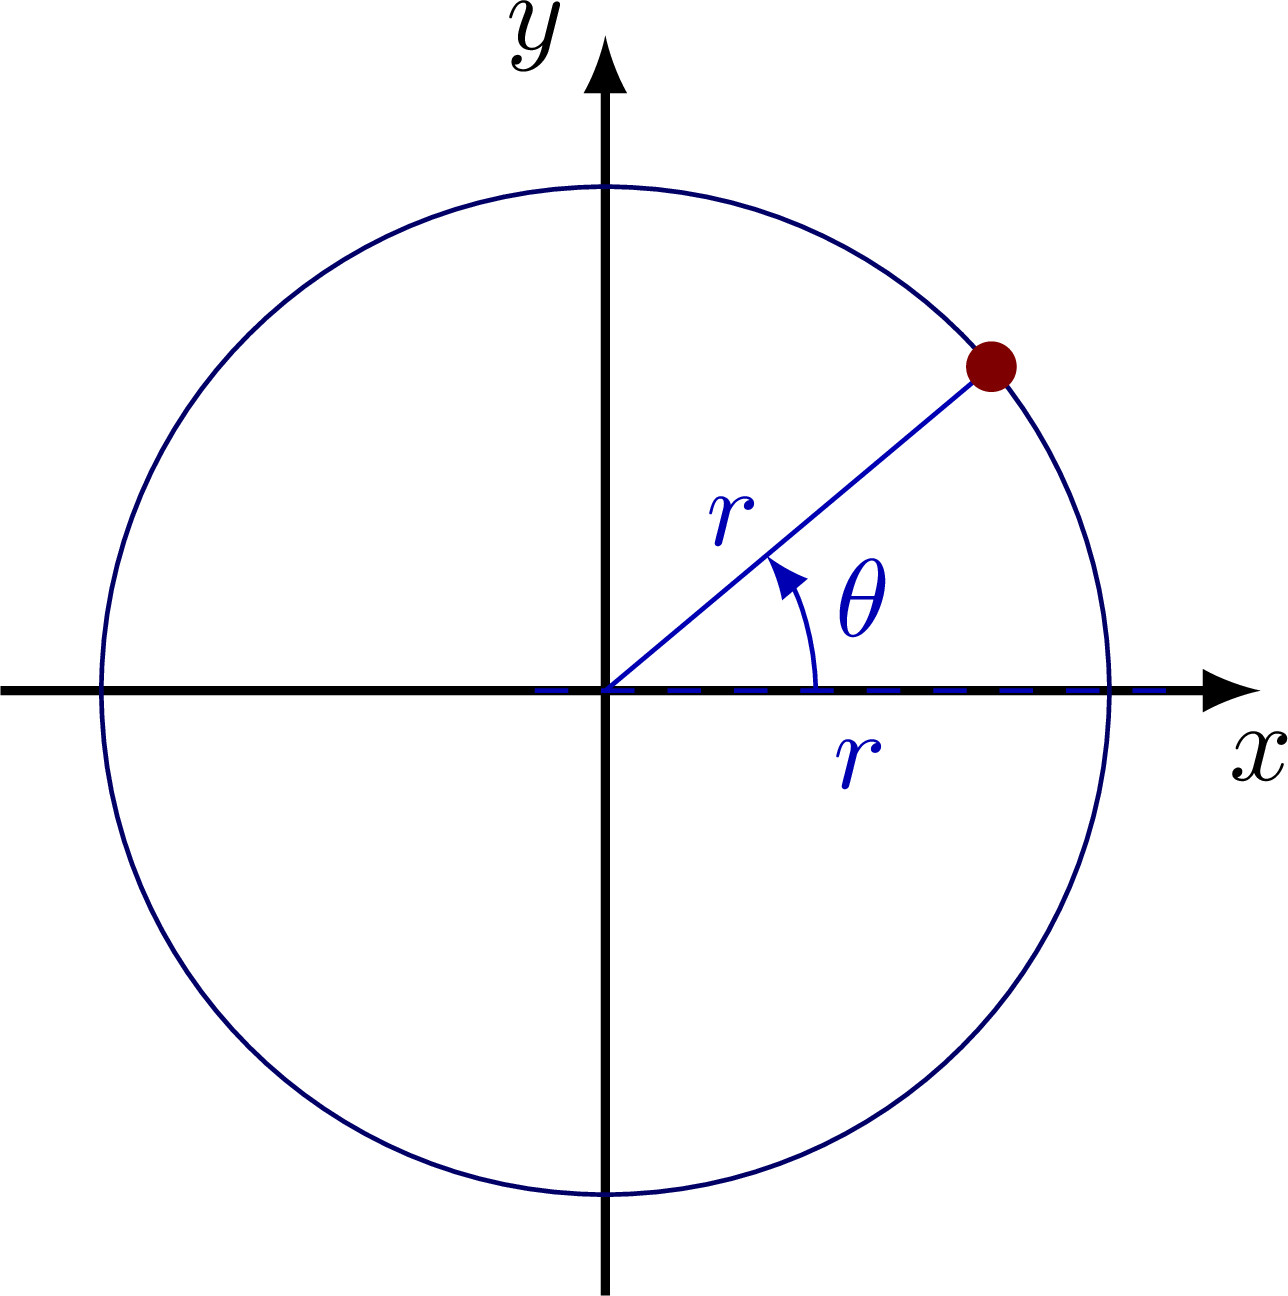
\includegraphics[width=0.45\textwidth]{image/posizioneAngolare.png}
    \caption{Posizione angolare}
    \label{fig:posizAng}
\end{figure}

\paragraph{}

\textbf{Velocità angolare:}\\

Al passare del tempo la posizione angolare del punto materiale che si muove su una traiettoria circolare cambia e dunque lo spostamento angolare $\Delta\theta$ del punto materiale è:

\begin{equation}
    \Delta\theta = \Delta_f - \Delta_i
\end{equation}

\begin{figure}
    \centering
    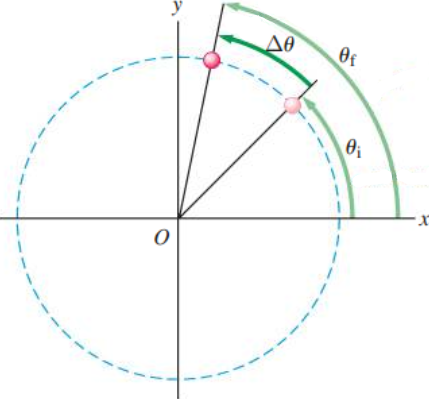
\includegraphics[width = 0.45\textwidth]{image/velocitaAng.png}
    \caption{Velocità angolare}
    \label{fig:velAng}
\end{figure}

Se dividiamo lo spostamento angolare per l’intervallo del tempo durante il quale avviene lo spostamento, otterremo la velocità angolare media:

\begin{equation}
    \omega_m = \frac{\Delta\theta}{\Delta t} \quad \biggl[\frac{rad}{s}\biggl]
\end{equation}

La velocità istantanea invece è: 

\begin{equation}
    \omega = \lim_{\Delta t \to 0} {\frac{\Delta\theta}{\Delta t}} \quad \biggl[\frac{rad}{s}\biggl]
\end{equation}

Questa definizione è analoga a quella della velocità istantanea lineare trattata in precedenza, si veda: \ref{velocitaLineare}

\paragraph{}
\textbf{Accelerazione tangenziale:}\\

Essendo che questo è un moto circolare uniforme allora l'accelerazione è nulla:

\begin{equation}
    \alpha = 0
\end{equation}


\paragraph{}
\textbf{Velocità tangenziale:}\\

Il modulo della velocità tangenziale $\vec{v}$ di un punto materiale è:

\begin{equation}
    v = \lim_{\Delta t \to 0}\frac{\Delta s }{\Delta t}  = \lim_{\Delta t \to 0}\frac{r\Delta \theta}{\Delta t} = \omega r \qquad \footnote{$\Delta s$ lung. del segmento che collega il punto al tempo $t_0$ con lo stesso punto al tempo $t_1$}
\end{equation}


\begin{figure}[H]
    \centering
    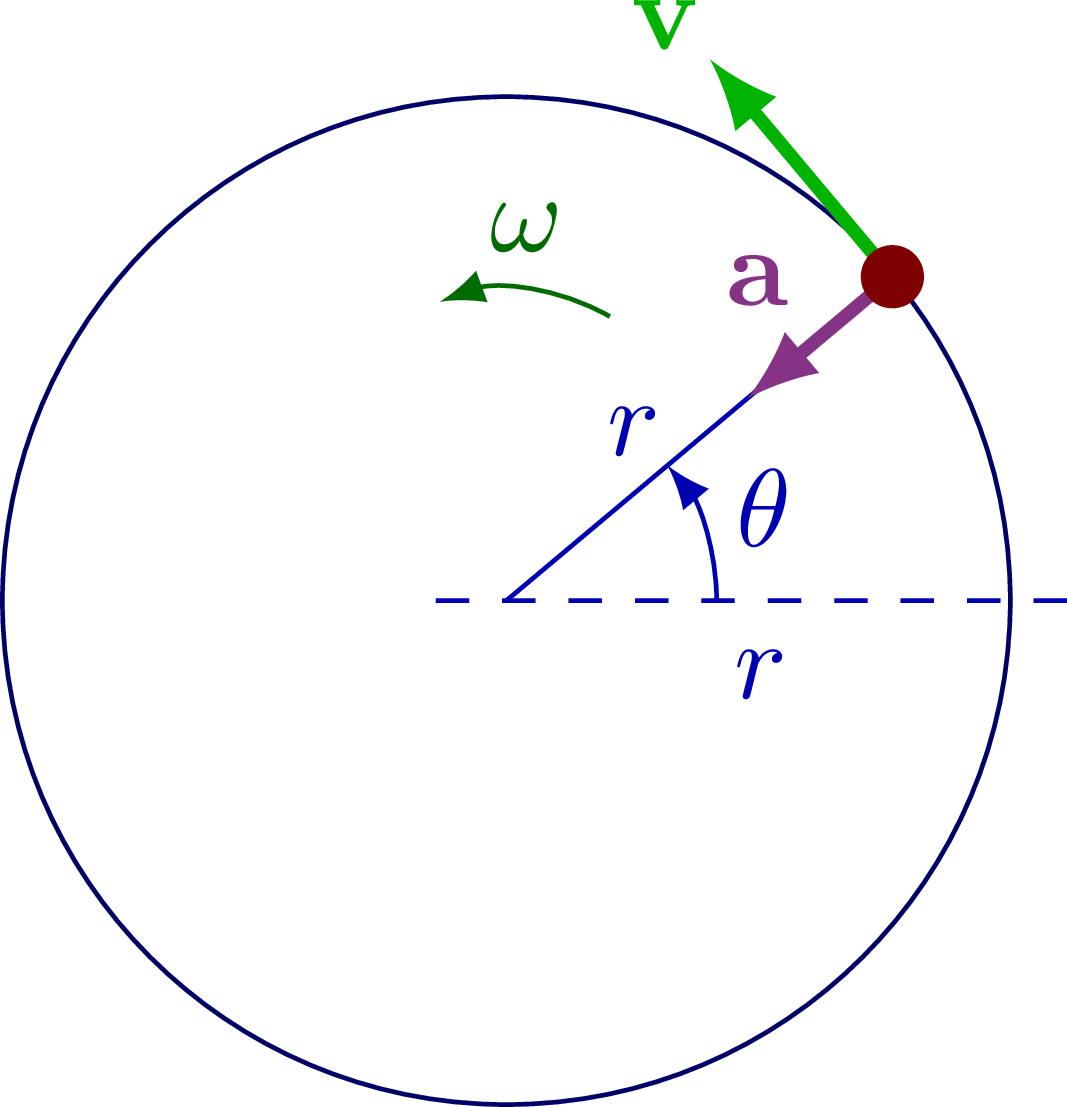
\includegraphics[width= 0.45 \textwidth]{image/motoCircUnif.png}
    \caption{Moto circolare uniforme}
    \label{fig:motoCircUnif}
\end{figure}

\paragraph{}
\textbf{Accelerazione centripeta:}\\

In particolare modo noi ci soffermeremo sul \textit{moto circolare uniforme},il quale ha velocità angolare e modulo delle velocità costanti, mentre la direzione varia essendo sottoposto ad un'accelerazione. Tale moto è un esempio di moto periodico, che si ripete ciclicamente nel tempo.
In un moto periodico $T$ è il tempo necessario per compiere un giro completo.

L'accelerazione costante viene chiamata \textit{accelerazione centripeta}, dal latino "diretta verso il centro". Figura \ref{fig:motoCircUnif}.

\paragraph{}
\textbf{Forza centrifuga}\\
\e una forza apparente applicata ad un oggetto massivo che gode di moto rotatorio. Questa è uguale in modulo e direzione opposta rispetto alla forza centripeta in un sistema inerziale, come in Figura \ref{fig:sistemaNonInerzialee}.

\def\R{2}      % disk radius
\def\t{0.1}    % disk thickness
\def\p{0.05}   % pole radius
\def\P{1.3}    % pole height
\def\r{0.24}   % mass radius
\def\L{0.7*\R} % rope length
\def\H{2.0}    % human height
\begin{figure}[H]
    \centering
    \begin{minipage}[c]{0.4\textwidth}
    
    \begin{tikzpicture}[scale = 1]
      \centering
      % PERSON
      \coordinate (H) at (0,\H);
      \draw[thick,line cap=round]
        (H)++(-165:0.3) to[out=-140,in=60]++ (-130:0.3)
        to[out=65,in=-90,looseness=1.0]++ (80:0.45) to[out=90,in=120,looseness=1.4]++ (20:0.2); % pony tail
      \draw[thick,fill=white] (H) circle (0.3);
      \draw[thick,line cap=round] (H)++(-140:0.3) to[out=80,in=-120,looseness=1.8]++ (40:0.6); % hair
      \draw[thick] (H)++(-90:0.3) coordinate (N) to[out=-95,in=95]++ (0,-0.40*\H) coordinate (P);
      \draw[thick,line cap=round] (N)++(-95:0.03) to[out=-60,in=95]++ (0.10*\H,-0.4*\H) coordinate (RH);
      \draw[thick,line cap=round] (N)++(-95:0.03) to[out=-120,in=90]++ (-0.08*\H,-0.4*\H);
      \draw[thick] (P) to[out=-70,in=95] (0.08*\H,0);
      \draw[thick] (P) to[out=-100,in=72] (-0.06*\H,0);
      
      % AXIS
      \node (A) at (0.38*\H,0.94*\H) {S};
      \draw[<->,line width=0.9]
        (A)++(0.25*\H,0.28*\H) node[left,scale=0.9] {$z$} --++ (0,-0.3*\H) coordinate (O) --++
             (0.3*\H,0) node[below right=-3.5,scale=0.9] {$y$};
      \draw[->,line width=0.9] (O) --++ (-120:0.25*\H) node[left=-2,scale=0.9] {$x$};
      
      % DISK
      \begin{scope}[shift={(0.5*\H+\R,0.3*\H)}]
        \coordinate (T) at (0,\r);
        \draw[disk] (-\R,0) --++ (0,-\t) arc(180:360:{\R} and {0.4*\R}) --++ (0,\t);
        \draw[disk] (0,0) ellipse({\R} and {0.4*\R});
        \rope {(T) --++ (\L,0) coordinate (M)};
        \draw[pole] (-\p,\P) --++ (0,-\P) arc(180:360:{\p} and {0.4*\p}) --++ (0,\P);
        \draw[pole] (0,\P) ellipse({\p} and {0.4*\p});
        \rope {(-1.4*\p,0.85*\r) arc(180:360:{1.4*\p} and {0.4*\p})}
        \rope {(-1.4*\p,1.00*\r) arc(180:360:{1.4*\p} and {0.4*\p})}
        \rope {(-1.4*\p,1.15*\r) arc(180:360:{1.4*\p} and {0.4*\p})}
        \draw[force] (M)++(150:1.1*\r) --++ (-0.5*\L,0) node[above=-1] {$\vb{T}$};
        \draw[avec] (M)++(210:1.1*\r) --++ (-0.5*\L,0) node[right=0,below=-1] {$\vb{a}$}; %_\mathrm{cm}
        \draw[mass] (M) circle(\r) node {$m$};
        \draw[->] (10:1.05*\R) arc(10:50:{1.05*\R} and {0.4*\R}) node[above left=-2] {$\omega$};
        \draw[vvec] (0,\P+0.014) --++ (0,0.7*\L) node[midway,left] {$\vb*\omega$};
      \end{scope}
      
    \end{tikzpicture}
    
    \caption{Sistema di riferimento inerziale}
    \label{fig:sistemaInerzialee}
    \end{minipage}
    \hspace{10mm}
    \begin{minipage}[c]{0.4\textwidth}
    \centering
    \begin{tikzpicture}[scale = 1]
  
      % DISK
      \coordinate (T) at (0,\r);
      \draw[disk] (-\R,0) --++ (0,-\t) arc(180:360:{\R} and {0.4*\R}) --++ (0,\t);
      \draw[disk] (0,0) ellipse({\R} and {0.4*\R});
      
      % PERSON
      \draw[thick,fill=white] (-0.35*\R,\H) circle (0.15*\H) coordinate (H);
      \draw[thick] (H)++(-90:0.15*\H) coordinate (N) to[out=-95,in=95]++ (0,-0.40*\H) coordinate (P);
      \draw[thick,line cap=round] (N)++(-95:0.03) to[out=-70,in=190]++ (0.34*\H,-0.20*\H);
      \draw[thick,line cap=round] (N)++(-95:0.03) to[out=-120,in=-80]++ (-0.17*\H,-0.12*\H) to[out=100,in=-100]++ (0.02*\H,0.25*\H);
      \draw[thick] (P) to[out=-70,in=95] ($(H)+(0.08*\H,-\H)$);
      \draw[thick] (P) to[out=-100,in=72] ($(H)+(-0.08*\H,-\H)$);
      
      % POLE + MASS
      \rope {(T) --++ (\L,0) coordinate (M)};
      \draw[pole] (-\p,\P) --++ (0,-\P) arc(180:360:{\p} and {0.4*\p}) --++ (0,\P);
      \draw[pole] (0,\P) ellipse({\p} and {0.4*\p});
      \rope {(-1.4*\p,0.85*\r) arc(180:360:{1.4*\p} and {0.4*\p})}
      \rope {(-1.4*\p,1.00*\r) arc(180:360:{1.4*\p} and {0.4*\p})}
      \rope {(-1.4*\p,1.15*\r) arc(180:360:{1.4*\p} and {0.4*\p})}
      \draw[force] (M)++(150:1.1*\r) --++ (-0.5*\L,0) node[above=-1] {$\vb{T}$};
      \draw[force] (M)++(30:1.1*\r) --++ (0.5*\L,0) node[above=0] {$\vb{F}_\mathrm{cf}$};
      \draw[mass] (M) circle(\r) node {$m$};
      
      % AXIS
      \node (A) at (57:0.88*\R) {S$'$};
      \draw[<->,line width=0.9]
        (A)++(0.25*\H,0.28*\H) node[left,scale=0.9] {$z'$} --++ (0,-0.3*\H) coordinate (O) --++
             (0.3*\H,0) node[below right=-3.5,scale=0.9] {$y'$};
      \draw[->,line width=0.9] (O) --++ (-120:0.25*\H) node[left=-2,scale=0.9] {$x'$};
      
    \end{tikzpicture}
    
    \caption{Sistema di riferimento non inerziale}
    \label{fig:sistemaNonInerzialee}
    \end{minipage}
\end{figure}


\paragraph{}
Di seguito vengono riportate tutte le formule utili.
\paragraph{}
\textbf{Legge oraria: }
\begin{equation}
    \theta = \theta_0 + \omega t
\end{equation}
\paragraph{}
Velocità tangenziale:
\begin{equation}
    v = \frac{2\pi r}{t} \qquad v = \omega r
\end{equation}

Velocità angolare:
\begin{equation}
    \omega = \frac{2\pi}{t}\qquad \omega = \frac{v}{r}
\end{equation}

Accelerazione angolare:
\begin{equation}
    \alpha = 0
\end{equation}

Accelerazione centripeta:
\begin{equation}
    a_c = \frac{v^2}{r}\qquad a_c=\omega^2r
    \label{AccelerazioneCentripeta}
\end{equation}

Forza centrifuga:
\begin{equation}
    F_c = \frac{mv^2}{r}\qquad F_c=m\omega^2r
\end{equation}

Frequenza:
\begin{equation}
    f = \frac{1}{T}
\end{equation}



\section{Moto Rotatorio}
Un corpo si dice che è in moto rotatorio se esso ruota su sé stesso.
Ogni punto di un corpo rigido rotante attorno ad un asse descrive una traiettoria circolare e pertanto segue le leggi del \textit{Moto circolare}.
Consideriamo una ruota di bicicletta, Figura \ref{fig:ruotaBici}, libera di ruotare al proprio asse, come mostrato in figura.

Quando la ruota gira, ogni suo punto si muove su una traiettoria circolare il cui centro è l’asse di rotazione.


\begin{figure}[H]
    \centering
    \def\R{1.6} % wheel rims inside
    \begin{tikzpicture}
      \def\ang{90} % angle
      \def\F{1.2}  % force size
      \coordinate (O) at (0,0);
      \coordinate (R) at (\ang:\R);
      \clip (-1.2*\Rr,-1.17*\Rr) rectangle (1.17*\Rr,1.54*\Rr);
      \wheel
      \draw[rvec] (O) -- (\ang:0.95*\R) node[midway,above=3,right=-1] {\contour{white}{$\vb{r}$}};
    \end{tikzpicture}
    \caption{Ruota di bicicletta}
    \label{fig:ruotaBici}
\end{figure}

\newpage



\newpage
\chapter{Energia}
Fino a questo punto, in tutti gli esercizi, abbiamo fatto largo uso del tempo per poter calcolare ciò che ci richiedeva il problema.
Questo approccio, però, è molto limitato perché le forze in generale non sono costanti nel tempo, ma sono costanti nello spazio \label{costantiSpazio}, come vedrete a seguito nella spiegazione di lavoro di una forza costante e variabile.

Essendo l’energia ovunque, sotto diverse forme, l'energia di un corpo, o sistema, è possibile trovarla prima che il moto succeda.

\section{Che cos'è l'energia? }
L’energia, in fisica, è una grandezza che esprime la capacità di un corpo, o di un sistema, di compiere un lavoro, ed è associata ad una grandezza scalare: il Joule $[J = Nm]$
\paragraph{}
Ci sono diversi tipi di energia, in particolare a noi ne interessano tre:

\begin{itemize}
    \item Energia cinetica $E_c$
    \item Energia potenziale $E_p$
    \item Energia meccanica $E_{tot}$
\end{itemize}

Dove l’energia meccanica è definita come la somma di energia cinetica e di energia potenziale dello stesso sistema. 

\newpage
\subsection{Il lavoro compiuto da una forza costante}

\begin{figure}[tb]
    \centering
    \begin{tikzpicture}[scale = 1.3]
      \def\ul{0.52}
      \def\R{3.1}
      \def\ang{26}
      \coordinate (O) at (0,0);
      \coordinate (R) at (\ang:\R);
      \coordinate (X) at ({\R*cos(\ang)},0);
      \draw[projcol,dashed] (R) -- (X);
      \draw[vector] (O) -- (R) node[midway,left=5,above right=0] {$\vec{A}$};
      \draw[vector,projcol]
        (O) -- (X) node[scale=0.8,left=4,below=-1] {$\vec{A}\text{x}\vec{B} = AB\cos\theta$};
      \draw[vector,unitcol]
        (O) -- (\ul,0) node[scale=0.9,left=2,below left=0] {$\vec{B}$};
      \draw pic[->,thick,"$\theta$",draw=black,angle radius=26,angle eccentricity=1.3]
        {angle = X--O--R};
    \end{tikzpicture}
    \caption{Prodotto Scalare}
    \label{fig:prodScalare}
\end{figure}

Per svolgere i calcoli rispolveriamo il concetto di prodotto scalare tra due vettori:

\begin{equation*}
    \vec{A}\cdot \vec{B} = AB\cos\theta
\end{equation*}

Il risultato è uno scalare, un numero, che rappresenta la proiezione del vettore $\vec{A}$ sul vettore $\vec{B}$ come è raffigurato nella Figura \ref{fig:prodScalare}.

Data una forza costante $\vec{F}$ esercitata su un corpo che effettua uno spostamento rettilineo $\vec{s}$, possiamo scrivere la formula del lavoro:

\begin{equation*}
    L = \vec{F} \cdot \vec{s}
\end{equation*}

Essendo che la forza e lo spostamento sono vettori, il prodotto della formula precedente è un prodotto scalare e dunque possiamo scrivere equivalentemente:

\begin{equation}
    L = Fs\cos\theta
    \label{lavoroForzaConst}
\end{equation}

\begin{figure}[H]
    \centering
    
    \begin{tikzpicture}[scale = 1.3]
      \def\W{2.7}  % ground width
      \def\D{0.2}  % ground depth
      \def\h{0.8}  % mass height
      \def\w{1.0}  % mass width
      \def\F{1.1}  % force magnitude
      \def\ang{30} % angle force
      \coordinate (F0) at (0.4*\w,0.85*\h);
      \coordinate (Fx) at ($(F0)+({\F*cos(\ang)},0)$);
      \coordinate (F)  at ($(F0)+(\ang:\F)$);
      \draw[ground] (-0.3*\W,0) rectangle++ (\W,-\D);
      \draw (-0.3*\W,0) --++ (\W,0);
      \draw[mass] (-\w/2,0) rectangle++ (\w,\h) node[midway] {$m$};
      \draw[force,xcol] (\w/2,0.15*\h) --++ (0.4*\W,0) node[midway,above=-1.5] {$\vb*{s}$};
      \draw[dashed,myred!80!black!60] (Fx) -- (F);
      \draw[Fproj] (F0) -- (Fx) node[above=1,right=-1] {$F\cos\theta$}; %\vu{x}
      \draw[force] (F0) -- (F)  node[above=1,right=-1] {$\vec{F}$};
      \draw pic["$\theta$",draw=black,angle radius=14,angle eccentricity=1.4] {angle=Fx--F0--F};
    \end{tikzpicture}
    \caption{Lavoro di un corpo sottoposto ad una forza $\vec{F}$}
    \label{fig:lavoroCorpoSottopostoForza}
\end{figure}

\subsection{Il lavoro compiuto da una forza variabile}

Per introdurre la nozione di lavoro compiuto da una forza variabile consideriamo uno spostamento unidirezionale lungo l’asse X e la forza F in funzione dello spostamento. 

Immaginiamo ora di suddividere lo spostamento in tanti piccoli intervalli in modo da considerare la forza costante in ciascuno di essi. Figura \ref{lavoro}.
\paragraph{}
Dunque il lavoro totale sarà la forza di ogni lavoro constante in ciascun intervallo: 

\begin{equation*}
    L \simeq \Delta L_1 + \Delta L_2 + \dots +  \Delta L_n = F_1\Delta_x + F_2\Delta_x + \dots + F_n\Delta_x
\end{equation*}
\begin{equation}
    L \simeq \sum_{k = 1} ^ n F_k \Delta_x
\end{equation}


Siccome vogliamo calcolare precisamente il lavoro, dobbiamo far tendere a zero l'intervallo $\Delta_x$. Per ottenere il risultato voluto utilizziamo la nozione di limite:
\begin{equation}
    L = \lim_{\Delta_x \to 0} \sum_{k = 1} ^ n F_k \Delta_x
    \label{limiteIntervalloInfinitesimoLavoro}
\end{equation}

Questa formula altro non è che:

\begin{equation}
    L = \int_{x_1}^{x_2} F(x) \, dx = E_{(p_2)} - E_{(p_1)}
\end{equation}

Svolgendo i calcoli si ottiene che:
\begin{equation*}
    L = \int_{x_1}^{x_2} F(x) \, dx = F[x]_{x_1}^{x_2} = F(x_2 - x_1) = Fs
\end{equation*}

La differenza tra posizione finale e posizione iniziale è proprio uguale allo spostamento e dunque ci siamo ricondotti alla formula del lavoro di una forza costante: \ref{lavoroForzaConst}.

Tutto questo per spiegare perché a Pagina~\pageref{costantiSpazio} ho affermato che: "le forze in generale non sono costanti nel tempo, ma sono
costanti nello spazio".


\begin{figure}[tb]
    \centering
    % WORK diagram - curve
\def\xmax{3.4}
\def\ymax{2.2}
\begin{tikzpicture}[scale = 1.3]
  \def\x{.58*\xmax}
  \def\dx{.07*\xmax}
  \def\F{.75*\ymax}
  
  % AREA
  \coordinate (Ax) at (.12*\xmax,0);
  \coordinate (Cx) at (.84*\xmax,0);
  \coordinate (A) at (.12*\xmax,.55*\ymax);
  \coordinate (B) at (.48*\xmax,.80*\ymax);
  \coordinate (C) at (.84*\xmax,.60*\ymax);
  \fill[xcol!20] (A) to[out=10,in=180] (B) to[out=0,in=170] (C) |- (Ax) -- cycle;
  \path (Ax) -- (C) node[midway,left=-2,blue] {$L$};
  
  % LINE
  \draw[very thick,xcol] (A) to[out=10,in=180] (B) to[out=0,in=170] (C);
  \fill[xcol] (A) circle (0.04); %node[right=5,above=2] {$P_1$, $V_1$};
  \fill[xcol] (C) circle (0.04); %node[right=2] {$P_2$, $V_2$};
  
  % AXIS
  \draw[->,thick] (0,-0.1*\ymax) -- (0,\ymax); %node[left] {$F$};
  \draw[->,thick] (-0.1*\xmax,0) -- (\xmax,0) node[below] {$x$};
  \tick{Ax}{90} node[below] {$x_1$};
  \tick{Cx}{90} node[below] {$x_2$};
  \tick{0,\F}{0} node[left] {$F$};
  
  % RECTANGLE
  \draw[dashed] (0,\F) --++ (\x,0);
  \draw[xcol] (\x,0) rectangle++ (\dx,\F);
  \draw[smallarrow] (\x,-0.08) --++ (\dx,0) node[midway,below=0,scale=0.9] {$\Delta{x}$};
  %\node[below=-1] at (\x+\dx/2,0) {$\Delta x$};
  
\end{tikzpicture}
    \caption{Significato geometrico del lavoro}
    \label{lavoro}
\end{figure}

\subsection[Espressione generica del lavoro]{Espressione generica del lavoro con forze costanti e traiettoria qualsiasi}

\begin{figure}[H]
    \centering
    % CURVED PATH
    \begin{tikzpicture}
      \def\ul{0.6}
      \def\Ra{1.4}
      \def\Rb{0.8}
      \def\anga{0}
      \def\angb{25}
      \coordinate (A) at (0,0);
      \coordinate (B) at (1.1,1.9);
      \coordinate (C) at (2.1,1.0);
      \coordinate (D) at (3.7,0.4);
      \coordinate (E) at (5.1,2.1);
      
      \draw[xcol,thick]
        (A)++(-140:0.4) to[out=20,in=-120]
        (A) to[out=60,in=\anga-180]
        (B) to[out=\anga,in=100]
        (C) to[out=-80,in=\angb-180]
        (D) to[out=\angb,in=-120]
        (E) to[out=60,in=-160]++ (40:0.4);
      
      % PATH DIFFERENCE
      \draw[vector,acol]
        (B) --++ (\anga:0.5) coordinate (BS) node[above=2,right=-2] {$\vec{\dd r}$};
      \draw[vector,acol]
        (D) --++ (\angb:0.5) coordinate (DS) node[below right=-4] {$\vec{\dd r}$}; %above left=-4
      
      % FORCE
      \draw[force]
        (B) --++ (-80:0.8) coordinate (BF) node[below=-1] {$\vec{F}$};
      \draw[force]
        (D) --++ (145:0.6) coordinate (DF) node[above left=-3] {$\vec{F}$};
      \draw pic["$\theta$",draw=black,angle radius=6,angle eccentricity=1.8] {angle=BF--B--BS};
      \draw pic["$\theta$",draw=black,angle radius=6,angle eccentricity=1.8] {angle=DS--D--DF};
      
      \fill[xcol] (A) circle (2pt) node[above left=-1] {$A$};
      %\fill[xcol] (B) circle (2pt);
      %\fill[xcol] (C) circle (2pt);
      %\fill[xcol] (D) circle (2pt);
      \fill[xcol] (E) circle (2pt) node[below right=-1] {$B$};
      
    \end{tikzpicture}
    \caption{Lavoro di una forza variabile lungo una traiettoria qualsiasi}
    \label{fig:lavoroForzaVariabileLunoTraiettQualsiasi}
\end{figure}

Sappiamo che:
\begin{equation*}
    \vec{F} \cdot \vec{dr} = \text{Lavoro infinitesimo}
\end{equation*}

Per ottenere quindi il lavoro che farà un oggetto che si sposterà dal punto A al punto B nella Figura \ref{fig:lavoroForzaVariabileLunoTraiettQualsiasi} dobbiamo calcolare: 

\begin{equation}
    L = \int_{A}^{B} \vec{F} \cdot \vec{dr} = \int_{A}^{B} F \cos\theta \, dr \quad [J = Nm]
    \label{formulaGeneraleLavoro}
\end{equation}

\section{Energia Cinetica}
L'energia cinetica è una forma di energia legata al movimento dei corpi nello spazio, in particolare alla loro massa e alla loro velocità.
Per calcolare l'energia cinetica in un sistema si utilizza la seguente formula:

\begin{equation}
    E_c = \frac{1}{2}mv^2\quad  [J = Nm]
    \label{energiaCinetica}
\end{equation}
e le relative formule inverse: 
\begin{equation}
    m = \frac{2E_c}{v^2} \quad  [Kg]\qquad v = \sqrt{\frac{2E_c}{m}} \quad  \biggl[\frac{m}{s}\biggl]
\end{equation}

\subsection{Teorema delle forze vive}

La formula \ref{energiaCinetica} deriva dalla seguente dimostrazione del teorema chiamato \textit{Teorema delle forze vive} o \textit{Teorema dell'energia cinetica}.
\paragraph{}
Partiamo dalla definizione di lavoro utilizzando la seconda legge di Newton \ref{secondaLeggeNewton}: 

\begin{equation*}
    L = \vec{F}\cdot s = m\veca \cdot \vec{s}
\end{equation*}

Questa equazione può essere scritta sotto forma di spostamenti infinitesimi ($\vec{dr}$)

\begin{equation*}
   \vec{F}\cdot\vec{dr} = m\frac{d\vec{v}}{d\vec{t}}\cdot d\vec{r}
\end{equation*}

Osserviamo che $\frac{\vec{dr}}{\vec{dt}}$, uno spostamento infinitesimo su un tempo infinitesimo, corrisponde alla definizione di velocità $\vec{v}$ quindi  che il lavoro elementare è:
\begin{equation*}
    \vec{F}\cdot\vec{dr} = md\vec{v}\cdot \vec{v}
\end{equation*}

Per l'espressione generica del lavoro con forze costanti e traiettoria qualsiasi, possiamo definire il lavoro come la somma di tutti gli spostamenti inifinitesimi, da $A$ a $B$ 

\begin{equation*}
     \int_{A}^{B} \vec{F} \cdot \vec{dr} = \int_{v_i}^{v_f} md\vec{v}\cdot \vec{v}
\end{equation*}

\begin{equation*}
    = E_{(p_2)} - E_{(p_1)} = m \biggl[\frac{v^2}{2}\biggl]_{v_i}^{v_f}
\end{equation*}

\begin{equation*}
    = E_{(p_2)} - E_{(p_1)} = \frac{1}{2}mv_f^2 - \frac{1}{2}mv_i^2
\end{equation*}
\begin{equation}
    = \frac{1}{2}mv_i^2 + E_{(p_2)}  =  \frac{1}{2}mv_f^2 + E_{(p_1)}
\end{equation}

Questa risoluzione è vera se e solo se siamo in presenza di forze conservative, e quindi abbiamo che il lavoro è indipendente dal percorso ma dipende solo dallo spazio effettivamente percorso. Figura \ref{fig:lavoroCostante}.

\begin{figure}[tb]
    \centering
    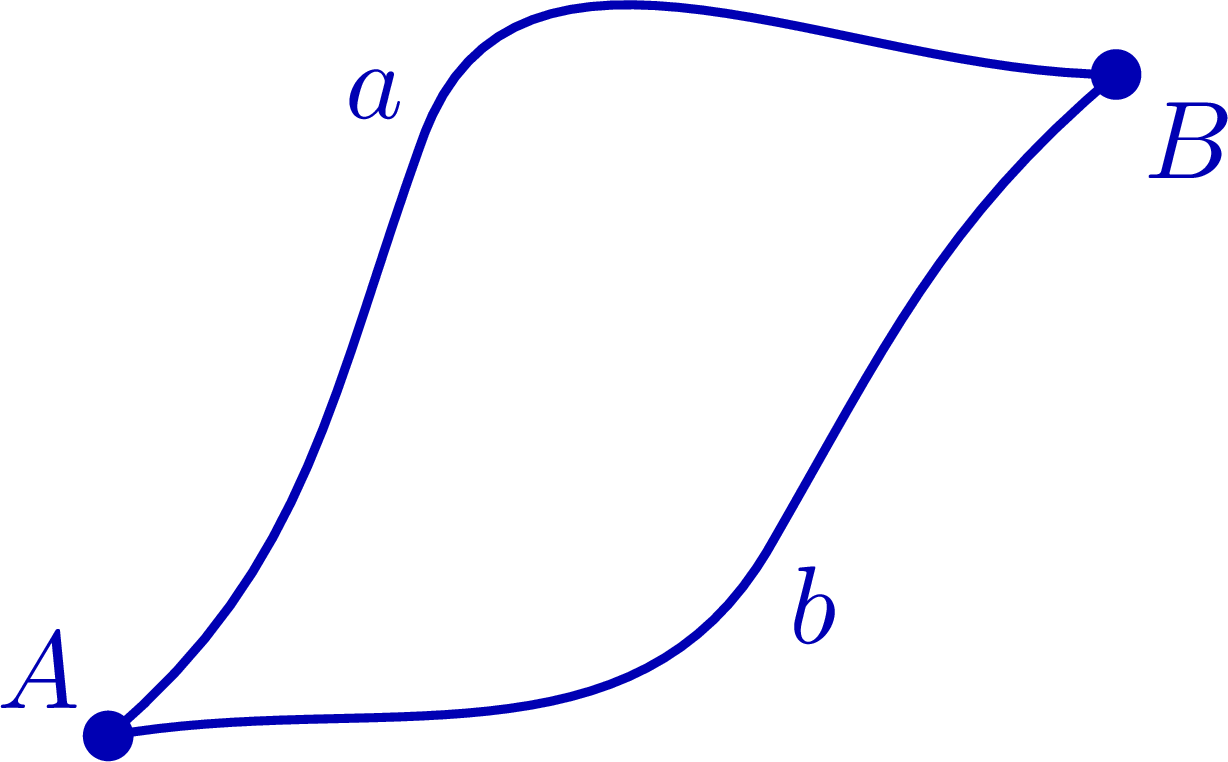
\includegraphics[width = 0.45 \textwidth]{image/lavoroNonDipDallaTraiett.png}
    \caption{Lavoro constante indipendentemente dal percorso scelto}
    \label{fig:lavoroCostante}
\end{figure}

\section{Energia Potenziale}
L'energia potenziale, $E_p$, è un tipo di energia che può essere associata solamente a corpi soggetti all'azione di forze conservative.
Essa è legata alla forza peso e all'altezza di caduta del corpo. Ha un limite: vale in prossimità della superficie terrestre.\\
Per definizione la variazione di energia potenziale è uguale al lavoro cambiato di segno: $\Delta E_p = -L$.\\
\paragraph{}
Per calcolare l'energia potenziale in un sistema si utilizza la seguente formula:
\begin{equation}
    E_p = mgh\quad[J = Nm]
    \label{energiaPotenziale}
\end{equation}

e le relative formule inverse:

\begin{equation}
    m = \frac{E_p}{gh}\quad[Kg] \qquad h= \frac{M_p}{mg}\quad\biggl[\frac{m}{s}\biggl]
\end{equation}

\paragraph{}
La formula \ref{energiaPotenziale} deriva dalla seguente dimostrazione.
\paragraph{}
Partiamo dalla formula della forza di gravità o forza peso:

\begin{equation*}
    \vec{F}=m\vec{g}
\end{equation*}
consideriamo $\vec{g}$ costante per quote vicine alla superficie terrestre.
Siccome la forza peso si esercita sempre verso il centro della terra, riscriviamo la forza considerando un sistema di riferimento con quote crescenti verso l'alto:
\begin{equation*}
    \vec{F}=-m\vec{g}
\end{equation*}

Utilizzando la definizione di energia potenziale, $\Delta E_p = -L$ otteniamo:

\begin{equation*}
     -L = \vec{F}\cdot\vec{dr}\footnote{$\vec{dr}$ rappresenta lo spostamento infinitesimo}
\end{equation*}

Dunque utilizzando gli integrai avremo che:

\begin{equation*}
     -\int_{h}^{0} dE_p = \int_{h}^{0} \vec{F} \cdot \vec{dr}
\end{equation*}
\begin{equation*}
    -[E_p]_h^0 = \int_{h}^{0} -mg dr
\end{equation*}
\begin{equation*}
     -E_p(0) + E_p(h) = mgh
\end{equation*}

\begin{equation}
    E_p(h) = E_p(0) + mgh
\end{equation}

\section{Energia Potenziale elastica}
L'energia potenziale elastica, $E_p$, è quell'energia che appartiene ad un corpo elastico come ad esempio la molla.
\e legata alla costante elastica $K$ e alla sua elongazione \footnote{Distanza lineare dalla posizione del copro in equilibrio}, l'energia potenziale elastica è sempre diretta in modulo opposto rispetto all'elongazione:

\begin{itemize}
    \item elongazione nulla, punto di equilibrio , $\Delta x = 0 \rightarrow$ forza nulla \hfill Figura \ref{fig:mollaAllung}
    \item elongazione positiva, allungamento, $\Delta x > 0 \rightarrow$ forza negativa \hfill Figura \ref{fig:mollaAllung}
    \item elongazione positiva, allungamento, $\Delta x < 0 \rightarrow$ forza positiva \hfill Figura \ref{fig:mollaAccoorc}
\end{itemize}

\paragraph{}
Per calcolare l'energia potenziale elastica in un sistema si utilizza la seguente formula:
\begin{equation}
    E_{pm} = \frac{1}{2}K(\Delta x)^2 \quad[J = Nm]
    \label{energiaPotenzialeElastica}
\end{equation}

e le relative formule inverse:

\begin{equation}
   K = \frac{2E_{pm}}{(\Delta x)^2}\quad\biggl[\frac{N}{m}\biggl] \qquad \Delta x = \sqrt{\frac{2E_{pm}}{K}}\quad[m]
\end{equation}

\paragraph{}
La formula \ref{energiaPotenzialeElastica} deriva dalla seguente dimostrazione:

Riprendendo la formula della forza elastica \ref{ForzaElastica} , $\vec{F_e} = -Kx $, e la definizione di energia potenziale $\Delta E_p = -L$ otteniamo:
\begin{equation*}
    \int_{x_0}^{0}-Kx\,dx = \int_{E_p(x_0)}^{E_p(0)} -dEp
\end{equation*}
\begin{equation*}
    -K\biggl[\frac{x^2}{2}\biggl]_{x_0}^{0} = -E_p(0) + E_p(x_0)
\end{equation*}
\begin{equation*}
    -K\biggl[\frac{x^2}{2}\biggl]_{x_0}^{0} = -E_p(0) + E_p(x_0)
\end{equation*}

L'energia potenziale elastica in $-E_p(0) = 0$, essendo la molla nel suo punto di equilibrio e dunque:
\begin{equation}
    K\frac{x_0^2}{2} = E_p(x_0)
\end{equation}


\begin{comment}
\begin{figure}
    \centering
    \begin{minipage}[c]{0.30\textwidth}
    \centering

        \begin{tikzpicture}
        
          \def\H{1.1}  % wall height
          \def\T{0.3}  % wall thickness
          \def\W{3.7}  % ground length
          \def\D{0.25} % ground depth
          \def\h{0.7}  % mass height
          \def\w{0.8}  % mass width
          \def\x{2.0}  % mass x position
          \def\y{1.22*\H} % x axis y position
          
          % AXIS
          \draw[mydashed] (\x,0.9*\h) --++ (0,\y-0.9*\h);
          \draw[axis] (\x-0.4*\W,\y) -- (\x+0.4*\W,\y) node[right] {$x$};
          \tick{\x,\y}{-90} node[scale=0.8,above=-1] {$0$};
          \draw[ell] (0,1.3*\h) --++ (\x,0) node[midway,fill=white,inner sep=0] {$\ell_0$};
          
          % SPRING & MASS
          \draw[spring] (0,\h/2) --++ (\x,0);
          \draw[ground] (0,0) |-++ (-\T,\H) |-++ (\T+\W,-\H-\D) -- (\W,0) -- cycle;
          \draw (0,\H) -- (0,0) -- (\W,0);
          \draw[mass] (\x,0) rectangle++ (\w,\h) node[midway] {$m$};
          
        \end{tikzpicture}
        
    \caption{Molla nel punto di equilibrio}
    \label{img:mollaEquilibrio}
    \end{minipage}
    \hspace{0.3mm}
    \begin{minipage}[c]{0.30\textwidth}
    \centering
        % HORIZONTAL spring - axis, extended
        \begin{tikzpicture}
          \def\H{1.1}  % wall height
          \def\T{0.3}  % wall thickness
          \def\W{3.9}  % ground length
          \def\D{0.25} % ground depth
          \def\h{0.7}  % mass height
          \def\w{0.8}  % mass width
          \def\x{2.0}  % mass x position
          \def\dx{0.8} % extension
          \def\y{1.22*\H} % x axis y position
          \def\F{0.8}  % force
          
          % AXIS
          \draw[mydashed] (\x,0) --++ (0,\y) (\x+\dx,0) --++ (0,1.1*\y);
          \draw[axis] (\x-0.4*\W,\y) -- (\x+0.4*\W,\y) node[right] {$x$};
          \tick{\x,\y}{-90} node[scale=0.8,above=-1] {$0$};
          \draw[ell] (0,1.3*\h) --++ (\x,0) node[midway,fill=white,inner sep=0] {$\ell_0$};
          \draw[dx] (\x,1.6*\h) --++ (\dx,0) node[pos=0.45,fill=white,inner sep=0] {$\Delta x$};
          
          % SPRING & MASS
          \draw[spring,segment length=7.5] (0,\h/2) --++ (\x+\dx,0);
          \draw[ground] (0,0) |-++ (-\T,\H) |-++ (\T+\W,-\H-\D) -- (\W,0) -- cycle;
          \draw (0,\H) -- (0,0) -- (\W,0);
          \draw[mass] (\x+\dx,0) rectangle++ (\w,\h) node[midway] {$m$};
          \draw[force] (\x+\dx+0.2*\w,0.9*\h) --++ (-\F,0) node[midway,right=1,above=-1] {$\vec{F}$};
          
        \end{tikzpicture}
    \caption{Molla allungata}
    \label{img:mollaAllungata}
    \end{minipage}
    \hspace{0.3mm}
    
    \begin{minipage}[c]{0.30\textwidth}
    \centering

% HORIZONTAL spring - axis, compressed
        \begin{tikzpicture}
          \def\H{1.1} % wall height
          \def\T{0.3} % wall thickness
          \def\W{3.9} % ground length
          \def\D{0.2} % ground depth
          \def\h{0.7} % mass height
          \def\w{0.8} % mass width
          \def\x{2.0} % mass x position
          \def\dx{0.9} % extension
          \def\y{1.22*\H} % x axis y position
          \def\F{0.8} % force
          
          % AXIS
          \draw[mydashed] (\x,0) --++ (0,\y) (\x-\dx,0) --++ (0,1.1*\y);
          \draw[axis] (\x-0.4*\W,\y) -- (\x+0.4*\W,\y) node[right] {$x$};
          \tick{\x,\y}{-90} node[scale=0.8,above=-1] {$0$};
          \draw[ell] (0,1.3*\h) --++ (\x,0) node[pos=0.4,fill=white,inner sep=0] {$\ell_0$};
          \draw[dx] (\x,1.6*\h) --++ (-\dx,0)
            node[pos=0.45,fill=white,inner sep=0,scale=0.9] {$\Delta x$};
          
          % SPRING & MASS
          \draw[spring,segment length=2.9] (0,\h/2) --++ (\x-\dx,0);
          \draw[ground] (0,0) |-++ (-\T,\H) |-++ (\T+\W,-\H-\D) -- (\W,0) -- cycle;
          \draw (0,\H) -- (0,0) -- (\W,0);
          \draw[mass] (\x-\dx,0) rectangle++ (\w,\h) node[midway] {$m$};
          \draw[force] (\x-\dx+0.8*\w,0.8*\h) --++ (\F,0) node[below=0,right=-1] {$\vec{F}$};
          
        \end{tikzpicture}
    
    \caption{Molla nel punto di equilibrio}
    \label{img:mollaEquilibrio}
    \end{minipage}
\end{figure}
\end{comment}

\begin{figure}[H]
    \centering
        % HORIZONTAL spring - axis, rest position
    \begin{tikzpicture}[scale = 1.3]
      \def\H{1.1}  % wall height
      \def\T{0.3}  % wall thickness
      \def\W{3.7}  % ground length
      \def\D{0.25} % ground depth
      \def\h{0.7}  % mass height
      \def\w{0.8}  % mass width
      \def\x{2.0}  % mass x position
      \def\y{1.22*\H} % x axis y position
      
      % AXIS
      \draw[mydashed] (\x,0.9*\h) --++ (0,\y-0.9*\h);
      \draw[axis] (\x-0.4*\W,\y) -- (\x+0.4*\W,\y) node[right] {$x$};
      \tick{\x,\y}{-90} node[scale=0.8,above=-1] {$0$};
      \draw[ell] (0,1.3*\h) --++ (\x,0) node[midway,fill=white,inner sep=0] {$\ell_0$};
      
      % SPRING & MASS
      \draw[spring] (0,\h/2) --++ (\x,0);
      \draw[ground] (0,0) |-++ (-\T,\H) |-++ (\T+\W,-\H-\D) -- (\W,0) -- cycle;
      \draw (0,\H) -- (0,0) -- (\W,0);
      \draw[mass] (\x,0) rectangle++ (\w,\h) node[midway] {$m$};
      
    \end{tikzpicture}
    \caption{Molla nel punto di equilibrio}
        \label{fig:mollaEquilibrio}
    
    % HORIZONTAL spring - axis, extended
    \begin{tikzpicture}[scale = 1.3]
      \def\H{1.1}  % wall height
      \def\T{0.3}  % wall thickness
      \def\W{3.9}  % ground length
      \def\D{0.25} % ground depth
      \def\h{0.7}  % mass height
      \def\w{0.8}  % mass width
      \def\x{2.0}  % mass x position
      \def\dx{0.8} % extension
      \def\y{1.22*\H} % x axis y position
      \def\F{0.8}  % force
      
      % AXIS
      \draw[mydashed] (\x,0) --++ (0,\y) (\x+\dx,0) --++ (0,1.1*\y);
      \draw[axis] (\x-0.4*\W,\y) -- (\x+0.4*\W,\y) node[right] {$x$};
      \tick{\x,\y}{-90} node[scale=0.8,above=-1] {$0$};
      \draw[ell] (0,1.3*\h) --++ (\x,0) node[midway,fill=white,inner sep=0] {$\ell_0$};
      \draw[dx] (\x,1.6*\h) --++ (\dx,0) node[pos=0.45,fill=white,inner sep=0] {$\Delta x$};
      
      % SPRING & MASS
      \draw[spring,segment length=7.5] (0,\h/2) --++ (\x+\dx,0);
      \draw[ground] (0,0) |-++ (-\T,\H) |-++ (\T+\W,-\H-\D) -- (\W,0) -- cycle;
      \draw (0,\H) -- (0,0) -- (\W,0);
      \draw[mass] (\x+\dx,0) rectangle++ (\w,\h) node[midway] {$m$};
      \draw[force] (\x+\dx+0.2*\w,0.9*\h) --++ (-\F,0) node[midway,right=1,above=-1] {$\vb{-F}$};
      
    \end{tikzpicture}
    \caption{Molla allungata}
        \label{fig:mollaAllung}
    
    % HORIZONTAL spring - axis, compressed
    \begin{tikzpicture}[scale = 1.3]
      \def\H{1.1} % wall height
      \def\T{0.3} % wall thickness
      \def\W{3.9} % ground length
      \def\D{0.2} % ground depth
      \def\h{0.7} % mass height
      \def\w{0.8} % mass width
      \def\x{2.0} % mass x position
      \def\dx{0.9} % extension
      \def\y{1.22*\H} % x axis y position
      \def\F{0.8} % force
      
      % AXIS
      \draw[mydashed] (\x,0) --++ (0,\y) (\x-\dx,0) --++ (0,1.1*\y);
      \draw[axis] (\x-0.4*\W,\y) -- (\x+0.4*\W,\y) node[right] {$x$};
      \tick{\x,\y}{-90} node[scale=0.8,above=-1] {$0$};
      \draw[ell] (0,1.3*\h) --++ (\x,0) node[pos=0.4,fill=white,inner sep=0] {$\ell_0$};
      \draw[dx] (\x,1.6*\h) --++ (-\dx,0)
        node[pos=0.45,fill=white,inner sep=0,scale=0.9] {$\Delta x$};
      
      % SPRING & MASS
      \draw[spring,segment length=2.9] (0,\h/2) --++ (\x-\dx,0);
      \draw[ground] (0,0) |-++ (-\T,\H) |-++ (\T+\W,-\H-\D) -- (\W,0) -- cycle;
      \draw (0,\H) -- (0,0) -- (\W,0);
      \draw[mass] (\x-\dx,0) rectangle++ (\w,\h) node[midway] {$m$};
      \draw[force] (\x-\dx+0.8*\w,0.8*\h) --++ (\F,0) node[below=0,right=-1] {$\vb{+F}$};
      \end{tikzpicture}
    \caption{Molla accorciata}
    \label{fig:mollaAccoorc}
\end{figure}

\section{Energia meccanica}
Energia meccanica, indicata con il simbolo $E$, è la somma dell’energia cinetica e dell’energia potenziale. Solo in presenza di forze conservative vale il principio di conservazione dell’energia secondo cui l’energia meccanica  ($E$ o $E_{tot}$) si conserva.

\begin{equation}
    E = E_p + E_c
\end{equation}

Infatti:
Il lavoro dell'energia cinetica e potenziale è così definito:

\begin{equation*}
    L = E_{cf} - E_{ci} \qquad -L = E_{pf} - E_{pi}
\end{equation*}

da cui: 

\begin{equation*}
    E_{cf} - E_{ci} = -E_{pf} + E_{pi}
\end{equation*}
\begin{equation*}
    E_{cf} + E_{pf} = E_{pi} + E_{ci}
\end{equation*}
\begin{equation}
    E_f = E_i
\end{equation}

Quindi abbiamo trovato che la somma dell'energia cinetica e potenziale, allo stato iniziale, è uguale alla somma dell'energia cinetica e potenziale allo stato finale.


\section{Potenza}
La potenza in Fisica, indicata con il simbolo $P$, è una grandezza legata al concetto di lavoro che fornisce una misura di quanto lavoro è stato svolto in un'unità di tempo.
Nel SI l'unità di misura della potenza è il Watt, $W = \frac{J}{s}$.

Il termine potenza o $W$ che comunemente viene utilizzato nel linguaggio comune, come ad esempio per compiere uno sforzo fisico o meccanico, non è molto diverso dal concetto fisico.

Per calcolare la potenza si utilizza la seguente formula:

\begin{equation}
    P = \frac{L}{\Delta t} = \frac{\vec{F} \cdot \vec{dr}}{dt} = \vec{F}\cdot \vec{v}\qquad \biggl[ W = \frac{J}{s}\biggl]
\end{equation}


\section{Pendolo semplice}

\def\L{2.8}  % string length
\def\ang{28} % angle string
\def\R{0.25} % ball radius
\def\F{1.0}  % force magnitude
\begin{figure}[H]
    \centering
    \begin{tikzpicture}
      \message{^^JPendulum}
      \coordinate (M) at (\ang-90:\L);
      \coordinate (M') at (0,-\L);
      \coordinate (O) at (0,0);
      \coordinate (B) at (0,-\L-2.2*\R);
      \coordinate (FT) at ($(M)+(90+\ang:{\F*cos(\ang)+\R})$);
      \coordinate (FG) at ($(M)+(-90:{\F+\R})$);
      \coordinate (FGx) at ($(M)+(-90+\ang:{0.55*\F+\R})$);
      \coordinate (MA) at ($(M)+(180+\ang:{\F*sin(\ang)+\R})$);
      %\draw[faded mass] (M') circle(\R);
      \draw[<->] (M)++(\ang-32:0.2*\L) node[below right=-1,scale=0.9] {$x$}
        --++ (\ang:0.17*\L) --++ (90+\ang:0.17*\L) node[above right=-1,scale=0.9] {$y$};
      \draw[dashed] (O) -- (B);
      %\draw[dashed,myred!60!black] (MA) -- (FG);
      \draw[dashed,myred!60!black] (M) -- (FGx);
      \draw[dashed] (-90+\ang+10:\L) arc(-90+\ang+10:-110:\L) (B);
      \rope{(O) -- (M)} \path (O) -- (M) node[midway,above right=-1] {$L$};
      \fill[black] (O) circle(0.04);
      \draw[force] (M) -- (FT) node[midway,left=0] {$\vb{T}$};
      \draw[force] (M) -- (FG) node[right=0] {$m\vb{g}$};
      \draw[force,acol] (M) -- (MA) node[right=2,below=0] {$m\vb{a}$}; %{\contour{white}{$m\vb{a}$}};
      \draw[mass] (M) circle(\R) node {$m$};
      \draw pic[myarr,"$\theta$",xcol,draw=xcol,angle radius=22,angle eccentricity=1.30] {angle=B--O--M}; %_\text{max}
      \draw pic[myarr,"$\theta$",xcol,draw=xcol,angle radius=14,angle eccentricity=1.45] {angle=FG--M--FGx};
    \end{tikzpicture}
    \caption{Pendolo semplice}
    \label{fig:pendoloSemplice}
\end{figure}

Il pendolo semplice è formato da una massa $m$ attaccato a un filo di lunghezza $L$. Il pendolo è in equilibrio stabile quando la massa si trova esattamente sotto al punto di sospensione e oscilla attorno a tale punto. 
Il pendolo gode di un moto armonico, ovvero impiega sempre lo stesso tempo a compiere un oscillazione completa.

\begin{figure}[H]
    \centering
    \begin{tikzpicture}[scale = 1.3]
      \message{^^JPendulum forces}
      \def\F{1.4}  % force magnitude
      \coordinate (O) at (0,0);
      \coordinate (FT) at (90+\ang:{\F*cos(\ang)});
      \coordinate (FG) at (-90:\F);
      \coordinate (FGx) at (-90+\ang:{\F*cos(\ang)});
      \coordinate (FGy) at (180+\ang:{\F*sin(\ang)});
      \draw[dashed,myred!60!black] (FGy) -- (FG); %-- (FGx);
      \draw[force] (O) -- (FT) node[midway,above right=-2] {$\vb{T}$};
      \draw[Fproj] (O) -- (FGy) node[pos=0.4,above left=-3,scale=0.86] {$mg\sin\theta$};
      \draw[Fproj] (O) -- (FGx) node[pos=0.5,above right=-3,scale=0.86] {$mg\cos\theta$};
      \draw[force] (O) -- (FG) node[right=0] {$m\vb{g}$};
      \draw pic[myarr,"$\theta$",xcol,draw=xcol,angle radius=14,angle eccentricity=1.45] {angle=FG--O--FGx};
    \end{tikzpicture}
    \caption{Forze applicate alla massa $m$ del pendolo in Figura \ref{fig:pendoloSemplice}}
    \label{fig:forzePendolo}
\end{figure}

\paragraph{}
Consideriamo ora le forze che agiscono sulla massa $m$, rappresentate nella figura \ref{fig:forzePendolo}.
Vediamo che sono rappresentate la forza peso e la tensione della filo. La tensione agisce in direzione radiale \footnote{Nella stessa direzione del raggio} e la sua intensità è uguale alla componente radiale del peso.

\begin{equation}
    T = mg\cos\theta
\end{equation}

La forza tangenziale che agisce sulla massa $m$ è sempre diretta verso il punto di equilibrio del pendolo: sotto al punto di sospensione.

\begin{equation}
    F = mg\sin\theta
\end{equation}

Inoltre per il \textit{Teorema dei piccoli angoli} fino a angoli di $30\gradi$ possiamo approssimare:
\begin{equation*}
    \sin\theta \approx \theta \qquad \text{$\theta$ è in radianti}
\end{equation*}

grazie agli sviluppi di Taylor:

\begin{equation*}
    \sin\theta = \theta - \frac{\theta^3}{6} + ...
\end{equation*}

Fermandoci al primo ordine avremo che:

\begin{equation*}
    \sin 30\gradi = 0.5 \quad\text{e dallo sviluppo ricaviamo}\quad 30\gradi  =  0,52 \,\text{Rad}
\end{equation*}

con un errore massimo di due centesimi, dato da $\frac{(\sin\theta)^3}{6} = 0.02$

\paragraph{}
Formule utili per la risoluzione dei problemi:
\paragraph{}
Velocità angolare:
\begin{equation}
    \omega = \sqrt{\frac{g}{L}}\quad \biggl[\frac{Rad}{s}\biggl]\qquad \omega = \sqrt{\frac{g}{L}}\frac{1}{2\pi}\quad \biggl[\frac{Giri}{s}\biggl]
\end{equation}

Periodo:
\begin{equation}
    P = 2\pi \sqrt{\frac{L}{g}} = \frac{2\pi}{\omega}
\end{equation}

Tensione \footnote{La tensione è massima quando $\theta = 0$}
\begin{equation}
    T = mg\cos\theta + mL\omega^2 = mg\cos\theta + m\frac{v^2}{L}
\end{equation}
viene usata l'accelerazione centripeta di pagina \pageref{AccelerazioneCentripeta}.
\paragraph{}
Conservazione dell'energia:
\begin{equation}
    mg(L-L\cos\theta_{max}) = \frac{1}{2}mv_{max}^2
\end{equation}
si veda la Figura \ref{fig:conservazioneEnergiaPendolo}
\paragraph{}
Velocità massima:
\begin{equation}
    v_{max} = \sqrt{2gL(1-\cos\theta_{max})}
\end{equation}

\def\L{2.8} % length
    \def\ang{32} % length
    \def\R{0.25} % ball radius
\begin{figure}[tb]
    \centering
    \begin{tikzpicture}[scale=1.3]
      \coordinate (M) at (\ang-90:\L);
      \coordinate (M') at (0,-\L);
      \coordinate (O) at (0,0);
      \coordinate (B) at (0,-\L-1.4*\R);
      \draw[faded mass] (M') circle(\R);
      \draw[dashed] (O) -- (B);
      \draw[dashed] (M')++(-0.7*\R,0) --++ ({0.65*\L*sin(\ang)},0) coordinate (A);
      \draw[dashed] (M')++(-0.7*\R,{\L-\L*cos(\ang)}) --++ ({1.2*\L*sin(\ang)},0);
      \draw[<->] (A)++(-0.2*\R,0) --++ (0,{\L-\L*cos(\ang)}) node[midway,right=-1] {$h$};
      \rope{(O) -- (M)} \path (O) -- (M) node[midway,right=1] {$L$};
      \fill[black] (O) circle(0.04);
      %\draw[force] (M)++(140:0.7*\r) --++ (-\F,0) node[below=1,above left=-4] {$\vb{F}_\mathrm{c}$};
      \draw[mass] (M) circle(\R) node {$m$};
      \draw pic[->,"\,$\theta_\text{max}$",xcol,draw=xcol,angle radius=29,angle eccentricity=1.3] {angle=B--O--M};
    \end{tikzpicture}
    \caption{Conservazione energia del pendolo}
    \label{fig:conservazioneEnergiaPendolo}
\end{figure}

\newpage
\section{Conservazione della quantità di moto}

Fino ad ora ci siamo interessati solo di come un corpo si muove su un piano soggetto a delle forze che agivano su di esso.
In questo capitolo ci concentreremo su cosa succede quando ci sono più corpi che interagiscono gli uni con gli altri per la terza legge di Newton \ref{terzaLeggeNewton}. 

Per prima cosa diamo la definizione di sistema: 
in fisica un sistema è un qualsiasi insieme di oggetti o punti materiali presi singolarmente. Esempio: un atomo o un pezzo continuo di materia come un cubo di lato 10 cm.

Questi punti materiali sono soggetti a forze interne e forze esterne:
\begin{itemize}
    \item Forza Interna: forza intrinsecamente presente nel sistema ($3^a$ Legge di Newton)
    \item Forza Esterna: forza applicata al di fuori del sistema, sono le interazioni esterne
\end{itemize}

La quantità di moto di un corpo di massa $m$ che si muove a velocità $\vec{v}$ è il vettore:

\begin{equation}
    \vec{p} = m\vec{v} \qquad\biggl[Kg\frac{m}{s}\biggl]
\end{equation}


\begin{figure}[H]
    \centering
    % GRAVITATIONAL ATTRACTION
    \begin{tikzpicture}
      \def\d{4.1}  % distance r
      \def\r{0.3}  % small radius ball
      \def\R{0.38} % large radius ball
      \def\RR{0.35} % large radius ball
      \def\F{0.95} % force magnitude
      \def\u{0.4}  % unit vector magnitude
      \def\ang{5}  % angle lin
      \coordinate (M1) at (0,0);
      \coordinate (M2) at (\ang:\d);
      \coordinate (M3) at (2,-1.8);
      
      % SETUP
      \draw[mass] (M1) circle(\r) node[scale=0.9] {$m_1$};
      \draw[mass] (M2) circle(\R) node[scale=0.9] {$m_2$};
      \draw[mass] (M3) circle(\RR) node[scale=0.9] {$m_3$};
      
      % FORCES
      \draw[force] (M1)++(\ang-8:0.9*\r) --++ (\ang:\F)
        node[anchor=90,inner sep=4] {$\vbF_{12}$}; % = -G\dfrac{m_1m_2}{r^2}\vu{r}_{21}
      \draw[force] (M2)++(\ang-172:0.9*\R) --++ (\ang:-\F)
        node[anchor=130,inner sep=3] {$\vbF_{21}$}; % = -G\dfrac{m_1m_2}{r^2}\vu{r}_{12}
        
        %est
        \draw[force] (M1)++(\ang0:0.3) --++ (\ang+25:0.9)
        node[anchor=90,inner sep=6] {$\vbF_{EST}$}; % = -G\dfrac{m_1m_2}{r^2}\vu{r}_{21}
        
        \draw[force] (M1)++(\ang-800:0.9*\r) --++ (\ang-50:0.9)
        node[anchor=20,inner sep=2] {$\vbF_{13}$}; % = -G\dfrac{m_1m_2}{r^2}\vu{r}_{21}
        
        %est
        \draw[force] (M2)++(\ang-80:0.4) --++ (\ang-100:0.9)
        node[anchor=90,inner sep=4] {$\vbF_{EST}$}; % = -G\dfrac{m_1m_2}{r^2}\vu{r}_{21}
      \draw[force] (M2)++(\ang99:0.9*\R) --++ (\ang-140:0.9)
        node[anchor=190,inner sep=10] {$\vbF_{23}$}; % = -G\dfrac{m_1m_2}{r^2}\vu{r}_{12}
        
        \draw[force] (M3)++(\ang+40:0.35) --++ (\ang+40:0.9)
        node[anchor=-250,inner sep=6] {$\vbF_{32}$}; % = -G\dfrac{m_1m_2}{r^2}\vu{r}_{21}
        
        %est
        \draw[force] (M3)++(\ang-150:0.35) --++ (\ang-190:0.9)
        node[anchor=90,inner sep=4] {$\vbF_{EST}$}; % = -G\dfrac{m_1m_2}{r^2}\vu{r}_{21}
      \draw[force] (M3)++(\ang-5:-0.35) --++ (\ang+130:0.9)
        node[anchor=190,inner sep=5] {$\vbF_{31}$}; % = -G\dfrac{m_1m_2}{r^2}\vu{r}_{12}
      
    \end{tikzpicture}
    \caption{Sistema di oggetti}
    \label{fig:sistemaOggetti}
\end{figure}


La forza totale che agisce sui corpi del sistema è la seguente:
\begin{equation*}
    m_1\veca_1 = \vec{F_{12}} + \vec{F_{13}} + \vec{F_{1est}}
\end{equation*}
\begin{equation*}
    m_2\veca_2 = \vec{F_{21}} + \vec{F_{23}} + \vec{F_{2est}}
\end{equation*}
\begin{equation*}
    m_3\veca_3 = \vec{F_{31}} + \vec{F_{32}} + \vec{F_{3est}}
\end{equation*}

tutte le coppie opposte si elidono e rimane solo:

\begin{equation*}
     m_1\veca_1 + m_2\veca_2+  m_3\veca_3 = \vec{F_{1est}} +\vec{F_{2est}} + \vec{F_{3est}}
\end{equation*}
\begin{equation}
    \sum_{i = 1} ^ 3 m_i\veca_i = \sum_{i = 1} ^ 3 m_i\vec{F_{iest}}
\end{equation}

Da questo capiamo che la somma delle forze interne è nulla e la quantità di moto totale dipende solo dalla somma delle forze esterne al sistema.
Quando siamo in presenza di un sistema isolato, cioè non è soggetto a forze esterne, allora anche la risultante della somma delle forze estere è nulla da cui abbiamo che:
\begin{equation}
    0 = \sum \vec{F_{int}} = \sum \vec{F_{est}} = 0
\end{equation}
Questo significa che la quantità di moto totale in un sistema isolato rimane costante:
\begin{equation}
    \vec{p}_{i-tot} = \vec{p}_{f-tot}
\end{equation}

\subsection{Il lavoro delle forze interne}
Le forze interne non alterano la quantità di moto totale di un sistema, ma in genere producono effetti sui singoli corpi che formano il sistema, infatti ogni variazione di energia cinetica corrisponde ad una variazione uguale di altre forze di energia all'intero del sistema stesso.
 Si pensi ad esempio ad un bagnino in piedi su una barca che lancia un salvagente, la barca acquista velocità ma a sua volta il salvagente compie un lavoro sul sistema barca + bagnino, che acquista energia cinetica. L’energia cinetica del salvagente è uguale all'energia chimica prodotta dai muscoli durante il lancio.
 
 \subsection{Centro di massa}
 La maggior parte degli oggetti comuni non sono punti, ma prendono le più svariate forme e dimensioni.
 In fisica questi corpi possono essere considerati come un sistema di corpi puntiformi e per analizzare il moto di un sistema di massa è utile considerare un particolare punto detto \textit{centro di massa} o \textit{baricentro}.
 
 La conservazione della quantità di moto ha un profondo effetto sui moti del baricentro, infatti questo punto si muove come il sistema puntiforme iniziale soggetto alle medesime forze esterne.
 
 Il baricentro di un sistema isolato si muove di moto rettilineo uniforme.
 
 \section{Urti}
 Un urto è un’interazione fra due corpi che vengono a contatto per un breve periodo di tempo.
 La conservazione della quantità di moto è uno strumento fondamentale per analizzare le dinamiche degli urti, permette di relazionare le velocità prima e dopo gli urti: in altri termini la quantità di moto del sistema immediatamente prima dell'impatto è uguale alla quantità di moto del sistema dopo l’impatto.
 
 \subsection{Urto anelastico}
 \e un urto dove non si conserva l’energia cinetica totale, in particolare se rimangono attaccati si parla di urto completamente anelastico e quindi i due corpi avranno la medesima velocità finale.
 
 La quantità di moto si conserva, energia cinetica non si conserva.
 
 \paragraph{}
 Formule per la risoluzione:
 \paragraph{}
 Urto anelastico:
\begin{equation}
    m_1\vec{v_1i} + m_2\vec{v_2i} = m_1\vec{v_1f} + m_2\vec{v_2f}
\end{equation}
nel caso l'urto sia anelastico si devono sapere tutte le quattro variabili dell'equazione precedente

\begin{figure}[H]
    \centering
    \def\w{0.8} % mass width
    \def\h{0.5} % mass height
    \def\v{0.7} % mass velocity
    \def\L{4.6} % length
    \begin{tikzpicture}
      \def\d{2.2} % distance
      \coordinate (M1) at (-\d/2+\w/2,0);
      \coordinate (M2) at (\d/2-\w/2,0);
      \draw[ground] (-\L/2,0) rectangle++ (\L,-0.2);
      \draw[thick] (-\L/2,0) --++ (\L,0);
      \draw[velocity] (M1)++(-\w/2,\h/2) --++ (-0.8*\v,0) node[left=-2] {$\vb{v}'_1$};
      \draw[velocity] (M2)++(\w/2,\h/2) --++ (1.2*\v,0) node[right=-2] {$\vb{v}'_2$};
      \draw[mass] (M1)++(-\w/2,0) rectangle++ (\w,\h) node[midway] {$m_1$};
      \draw[mass] (M2)++(-\w/2,0) rectangle++ (\w,\h) node[midway] {$m_2$};
      \pic[scale=1] at (0,0.5*\h) {collision={0.8}};
    \end{tikzpicture}
    \caption{Urto anelastico}
    \label{fig:UrtoAnelastico}
\end{figure}

\paragraph{}
 Urto completamente anelastico:
\begin{equation}
    m_1\vec{v_1i} + m_2\vec{v_2i} = (m_1+ m_2)\vec{v_f}
\end{equation}
in alcuni casi si deve mettere a sistema questa equazione con il moto rettilineo uniformemente accelerato \ref{leggeOrunifacc}

 \begin{figure}[H]
     \centering
     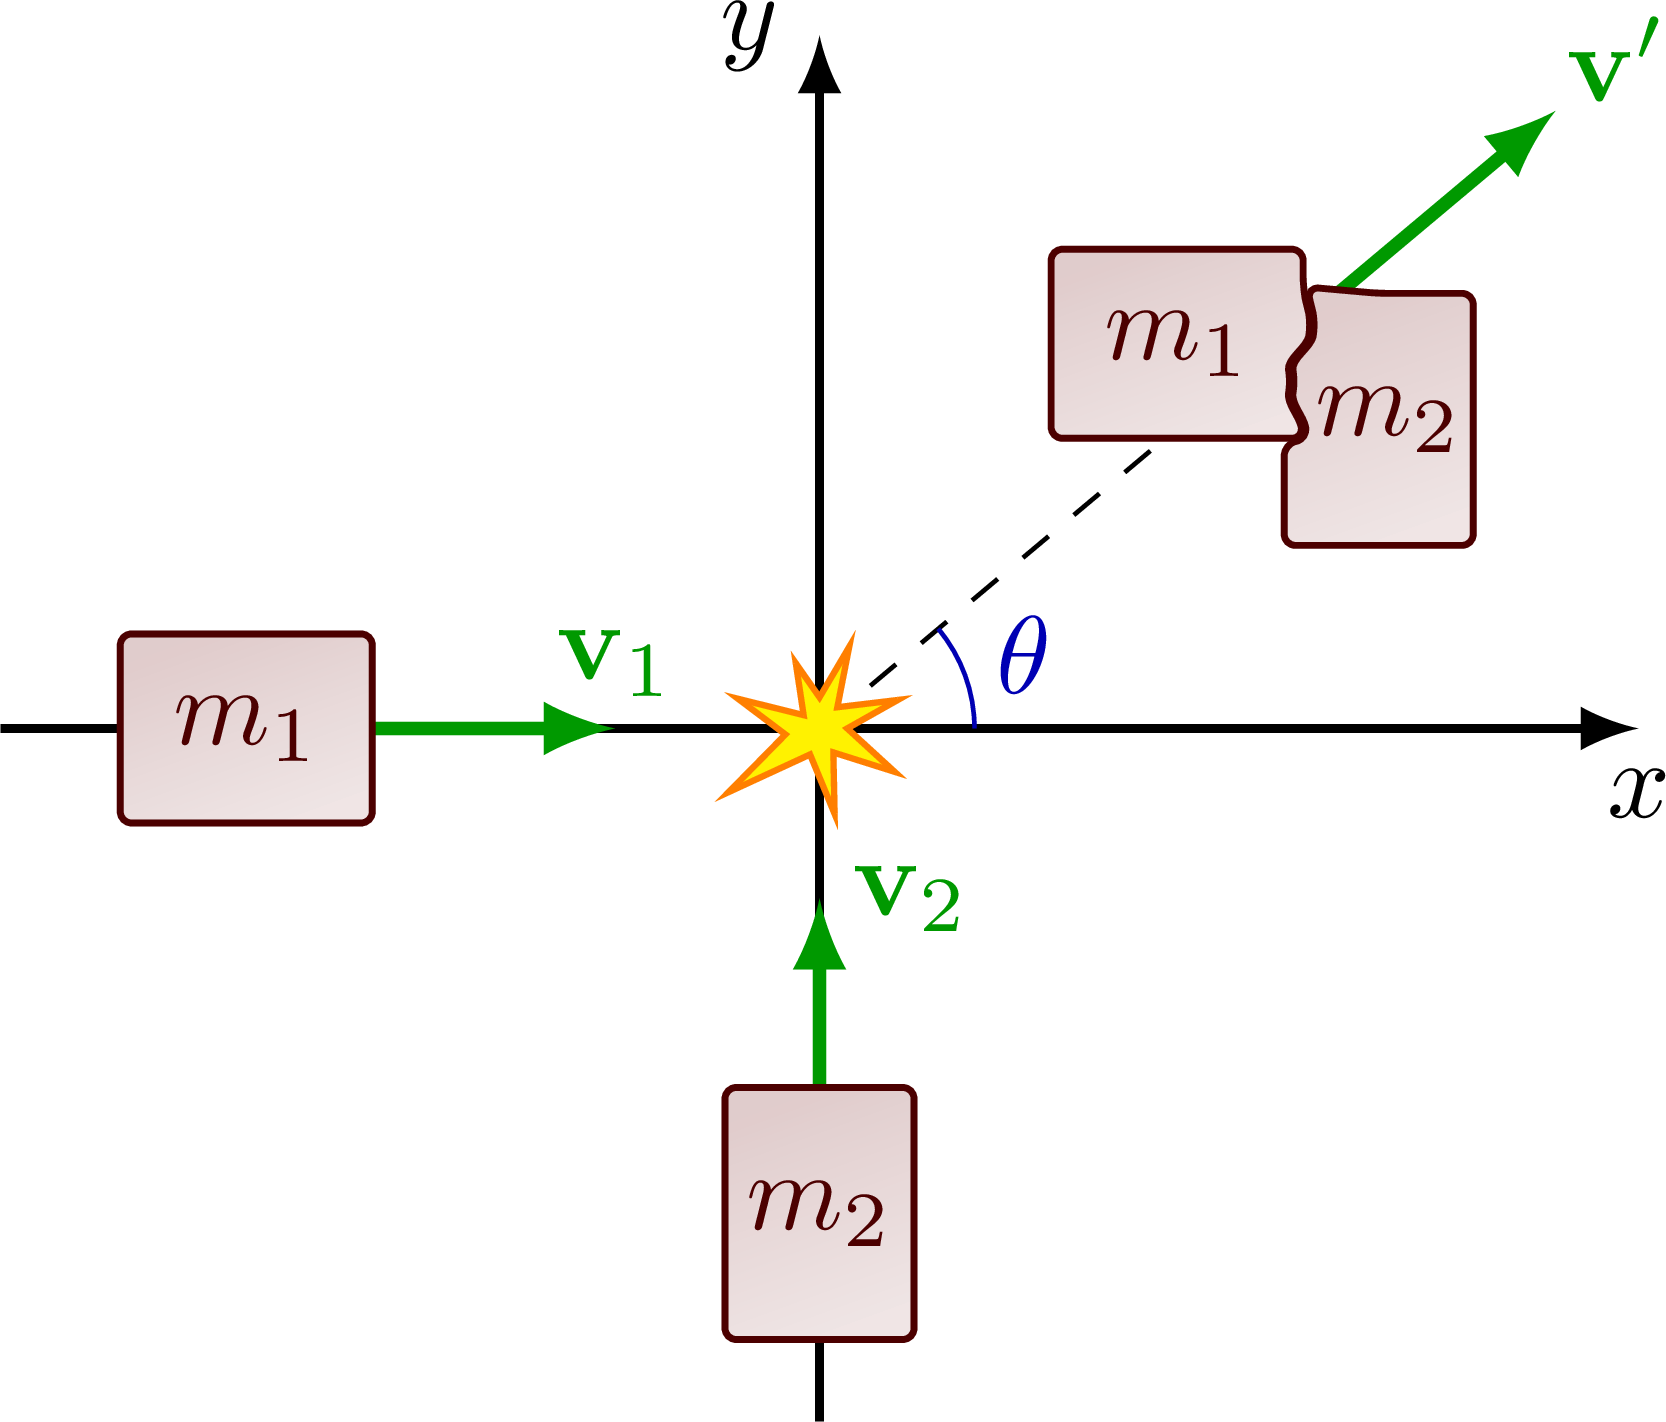
\includegraphics[width = 0.45\textwidth]{image/urtoAnelastico.png}
     \caption{Urto completamente anelastico}
     \label{fig:urtocompletamenteAnelastico}
 \end{figure}
 
\subsection{Urto elastico}
L’urto elastico è un urto dove si conserva sia la quantità di moto che l’energia cinetica. Si pensi al biliardo.

\paragraph{}
 Urto elastico:
$$
\begin{cases}

    m_1\vec{v_1i} + m_2\vec{v_2i} = m_1\vec{v_1f} + m_2\vec{v_2f}\\[10pt]
    \frac{1}{2}m_1\vec{v_1i}^2 + \frac{1}{2}m_2\vec{v_2i}^2  =\frac{1}{2}m_1\vec{v_1f}^2 + \frac{1}{2}m_2\vec{v_2f}^2
     
\end{cases}
$$

Mettiamo a sistema la quantità di moto con l'energia potenziale.

\paragraph{}
Troviamo le velocità finali dei due corpi:
$$
\begin{cases}

    v_{1f} = \frac{m1 -m2}{m1+m2}v_{1i} + \frac{2m_2}{m1+m2}v_{2i}\\[10pt]
    v_{2f} = \frac{m2 -m1}{m1+m2}v_{2i} + \frac{2m_1}{m1+m2}v_{1i}\\
     
\end{cases}
$$

Alcuni esempi...

\begin{figure}[H]
\centering
    \begin{minipage}[c]{0.45\textwidth}
    \centering
    % COLLISION 1D before
    \def\w{0.8} % mass width
    \def\h{0.5} % mass height
    \def\v{0.7} % mass velocity
    \def\L{4.6} % length
    \begin{tikzpicture}
      \def\d{3.8} % distance
      \coordinate (M1) at (-\d/2+\w/2,0);
      \coordinate (M2) at (\d/2-\w/2,0);
      \draw[ground] (-\L/2,0) rectangle++ (\L,-0.2);
      \draw[thick] (-\L/2,0) --++ (\L,0);
      \draw[velocity] (M1)++(\w/2,\h/2) --++ (1.1*\v,0) node[left=2,above=0] {$\vb{v}_1$};
      \draw[mass] (M1)++(-\w/2,0) rectangle++ (\w,\h) node[midway] {$m$};
      \draw[mass] (M2)++(-\w/2,0) rectangle++ (\w,\h) node[midway] {$m$};
    \end{tikzpicture}
    \caption{Urto elastico masse uguali, prima}
    \label{fig:urtoElasticoMasseUguali}
    \end{minipage}
    \hspace{0.1mm}
    \begin{minipage}[c]{0.45\textwidth}
    \centering
    % COLLISION 1D before
    \def\w{0.8} % mass width
    \def\h{0.5} % mass height
    \def\v{0.7} % mass velocity
    \def\L{4.6} % length
    \begin{tikzpicture}
      \def\d{3.8} % distance
      \coordinate (M1) at (-\d/2+\w/2,0);
      \coordinate (M2) at (\d/2-\w/2,0);
      \draw[ground] (-\L/2,0) rectangle++ (\L,-0.2);
      \draw[thick] (-\L/2,0) --++ (\L,0);
      \draw[mass] (M2)++(-\w/2,0) rectangle++ (\w,\h) node[midway] {$m$};
    \end{tikzpicture}
    \caption{Urto elastico masse uguali, dopo}
    \label{fig:urtoElasticoMasseUgualiDopo}
    \end{minipage}
    
\end{figure}

In Figura \ref{fig:urtoElasticoMasseUguali} viene rappresentato un urto elastico tra due blocchi di massa $m$.
Dopo l'urto, in accordo con le formule, troveremo che il blocco in movimento si sarà fermato ed avrà sostituito il posto del blocco fermo il quale ha iniziato a muoversi verso destra con velocità pari a $\vec{v_1}$.


\begin{figure}[H]
\centering
    \begin{minipage}[c]{0.45\textwidth}
    \centering
    % COLLISION 1D before
    \def\w{0.8} % mass width
    \def\h{0.5} % mass height
    \def\v{0.7} % mass velocity
    \def\L{4.6} % length
    \begin{tikzpicture}
      \def\d{3.8} % distance
      \coordinate (M1) at (-\d/2+\w/2,0);
      \coordinate (M2) at (\d/2-\w/2,0);
      \draw[ground] (-\L/2,0) rectangle++ (\L,-0.2);
      \draw[thick] (-\L/2,0) --++ (\L,0);
      \draw[velocity] (M1)++(\w/2,\h/2) --++ (1.1*\v,0) node[left=2,above=0] {$\vb{v}_1$};
      \draw[mass] (M1)++(-\w/2,0) rectangle++ (\w,\h) node[midway] {$M$};
      \draw[mass] (M2)++(-\w/2,0) rectangle++ (\w,\h) node[midway] {$m$};
    \end{tikzpicture}
    \caption{Urto elastico masse diverse, prima}
    \label{fig:urtoElasticoMasseDiversi}
    \end{minipage}
    \hspace{0.1mm}
    \begin{minipage}[c]{0.45\textwidth}
    \centering
    % COLLISION 1D before
    \def\w{0.8} % mass width
    \def\h{0.5} % mass height
    \def\v{0.7} % mass velocity
    \def\L{4.6} % length
    \begin{tikzpicture}
      \def\d{3.8} % distance
      \coordinate (M1) at (-\d/2+\w/2,0);
      \coordinate (M2) at (\d/2-\w/2,0);
      \draw[ground] (-\L/2,0) rectangle++ (\L,-0.2);
      \draw[thick] (-\L/2,0) --++ (\L,0);
    \end{tikzpicture}
    \caption{Urto elastico masse diverse, dopo}
    \label{fig:urtoElasticoMasseDiversiDopo}
    \end{minipage}
    
\end{figure}
In Figura \ref{fig:urtoElasticoMasseDiversi} viene rappresentato un urto elastico tra due blocchi di massa $M$ e massa $m$.
Dopo l'urto troveremo che il blocco in movimento, siccome molto più massivo dell'oggetto fermo, avrà travolto $m$ continuando ad una velocità pressoché inalterata a $\vec{v_1}$.

\begin{figure}[H]
\centering
    \begin{minipage}[c]{0.45\textwidth}
    \centering
    % COLLISION 1D before
    \def\w{0.8} % mass width
    \def\h{0.5} % mass height
    \def\v{0.7} % mass velocity
    \def\L{4.6} % length
    \begin{tikzpicture}
      \def\d{3.8} % distance
      \coordinate (M1) at (-\d/2+\w/2,0);
      \coordinate (M2) at (\d/2-\w/2,0);
      \draw[ground] (-\L/2,0) rectangle++ (\L,-0.2);
      \draw[thick] (-\L/2,0) --++ (\L,0);
      \draw[velocity] (M1)++(\w/2,\h/2) --++ (1.1*\v,0) node[left=2,above=0] {$\vb{v}_1$};
      \draw[mass] (M1)++(-\w/2,0) rectangle++ (\w,\h) node[midway] {$m$};
      \draw[mass] (M2)++(-\w/2,0) rectangle++ (\w,\h) node[midway] {$M$};
    \end{tikzpicture}
    \caption{Urto elastico masse diverse, prima}
    \label{fig:urtoElasticoMasseDiversi2}
    \end{minipage}
    \hspace{0.1mm}
    \begin{minipage}[c]{0.45\textwidth}
    \centering
    % COLLISION 1D before
    \def\w{0.8} % mass width
    \def\h{0.5} % mass height
    \def\v{0.7} % mass velocity
    \def\L{4.6} % length
    \begin{tikzpicture}
      \def\d{3.8} % distance
      \coordinate (M1) at (-\d/2+\w/2,0);
      \coordinate (M2) at (\d/2-\w/2,0);
      \draw[ground] (-\L/2,0) rectangle++ (\L,-0.2);
      \draw[thick] (-\L/2,0) --++ (\L,0);
      \draw[mass] (M2)++(-\w/2,0) rectangle++ (\w,\h) node[midway] {$M$};
      \draw[velocity] (M1)++(1.2,\h/2) --++ (-0.8*\v,0) node[left=-2] {$\vb{v}'_1$};
      \draw[mass] (M1)++(1.2,0) rectangle++ (\w,\h) node[midway] {$m$};
      \pic[scale=1] at (0.8,0.5*\h) {collision={0.8}};
    \end{tikzpicture}
    \caption{Urto elastico masse diverse, dopo}
    \label{fig:urtoElasticoMasseDiversiDopo2}
    \end{minipage}
    
\end{figure}

In Figura \ref{fig:urtoElasticoMasseDiversi2} viene rappresentato un urto elastico tra due blocchi di massa $m$ e massa $M$.
Dopo l'urto troveremo che il blocco in movimento, siccome molto meno massivo dell'oggetto fermo, avrà urtato contro $M$ e invertito la sua direzione mantenendo il modulo della velocità inalterato. 

\section{Momento angolare}

Il momento angolare di un punto materiale è una grandezza della dinamica rotazionale definita dal prodotto vettoriale tra il vettore posizione e il vettore quantità di moto.

Il momento angolare è il corrispondente rotazionale della quantità di moto e viene anche definito momento della quantità di moto.


\subsection{Prodotto vettoriale}
Per affrontare questo argomento bisogna fare un'introduzione al prodotto vettoriale. 
Il prodotto vettoriale è un’operazione tra vettori definita solo nello spazio tridimensionale. Tale operazione restituisce un nuovo vettore perpendicolare ai due vettori di partenza. Il verso di questo vettore risultante si determina con la cosiddetta regola della mano destra.
\paragraph{}
Come si vede dalla Figura \ref{fig:manoDx} dove l'indice indica il vettore $\vec{a}$ e il medio indica il vettore $\vec{b}$, portando l'indice verso il medio vediamo che il pollice assume automaticamente il verso del vettore risultante $\vec{a} \times \vec{b} = \vec{c}$

\begin{figure}[tb]
    \centering
    \begin{tikzpicture}[scale = 0.7]
      \coordinate (O) at (1.2,0.3); % ORIGIN
      \coordinate (WT) at ( 2.9,-1.1); % WRIST TOP
      \coordinate (T1) at ( 2.3, 0.7); % THUMB
      \coordinate (T2) at ( 1.75, 2.3);
      \coordinate (T3) at ( 2.0, 3.1);
      \coordinate (T4) at (1.38, 3.15);
      \coordinate (T5) at ( 0.9, 2.3);
      \coordinate (T6) at ( 0.85, 1.2);
      \coordinate (T7) at ( 0.85, 0.2);
      \coordinate (I1) at (-1.0, 2.4); % INDEX
      \coordinate (I2) at (-2.9, 3.45);
      \coordinate (I3) at (-3.3, 2.9);
      \coordinate (I4) at (-1.5, 1.8);
      \coordinate (I5) at (-0.9, 1.1);
      \coordinate (I6) at (-0.9, 0.5);
      \coordinate (M1) at (-2.2, 1.25); % MIDDLE
      \coordinate (M2) at (-3.9, 1.4);
      \coordinate (M3) at (-4.0, 0.8);
      \coordinate (M4) at (-2.3, 0.5);
      \coordinate (M5) at (-1.1, 0.25);
      \coordinate (R1) at (-1.9,-0.1); % RING
      \coordinate (R2) at (-1.8,-0.7);
      \coordinate (R3) at (-0.3,-1.5);
      \coordinate (R4) at ( 0.1,-1.7);
      \coordinate (R5) at ( 0.1,-1.0);
      \coordinate (R6) at (-0.5,-0.7);
      \coordinate (R7) at (-1.2,-0.3);
      \coordinate (P1) at (-1.9,-1.3); % PINKY
      \coordinate (P2) at (-0.8,-1.9);
      \coordinate (P3) at (-0.2,-2.1);
      \coordinate (P4) at (-0.05,-1.65);
      \coordinate (W1) at ( 0.4,-2.9); % WRIST BOTTOM
      \coordinate (W2) at ( 1.6,-3.5);
      
      % HAND
      \fill[brownskin]
        (WT) -- (T6) -- (I5) -- (M5) -- (R2) -- (P2) -- (W2) to[out=25,in=-90] cycle;
      \draw[fill=brownskin]
        (WT) to[out=120,in=-60] % THUMB
        (T1) to[out=120,in=-90]
        (T2) to[out=80,in=-110]
        (T3) to[out=80,in=50,looseness=1.5] % tip
        (T4) to[out=-130,in=80]
        (T5) to[out=-100,in=70]
        (T6) to[out=-100,in=100]
        (T7)
        (T6) to[out=150,in=-30] % INDEX
        (I1) to[out=150,in=-30]
        (I2) to[out=150,in=145,looseness=1.7] % tip
        (I3) to[out=-30,in=150]
        (I4) to[out=-30,in=105]
        (I5) to[out=-75,in=100]
        (I6)
        (I5) -- % MIDDLE
        (M1) --
        (M2) to[out=170,in=180,looseness=1.5] % tip
        (M3) to[out=-5,in=175]
        (M4) to[out=-5,in=165] % bottom knuckle
        (M5)
        (M5) to[out=-160,in=50] % RING
        (R1) to[out=-130,in=140,looseness=1.2]
        (R2) to[out=-30,in=160]
        (R3) --
        (R4) to[out=-20,in=-20,looseness=1.5] % tip
        (R5) --
        (R6) to[out=140,in=8,looseness=0.9]
        (R7)
        (R2) to[out=-160,in=155] % PINKY
        (P1) to[out=-35,in=150]
        (P2) to[out=-30,in=160]
        (P3) to[out=-20,in=-30,looseness=1.5] % tip
        %(P4) --
        (R4)
        (P2) to[out=-50,in=140] % WRIST
        (W1) to[out=-40,in=160]
        (W2);
      
      % FOLDS
      \draw[very thin] (T5)++(-80:0.3) to[out=40,in=180]++ (25:0.45);
      \draw[very thin] (I1)++(180:0.2) to[out=-160,in=100]++ (-130:0.6);
      \draw[very thin] (I1)++(155:1.3) to[out=-160,in=90]++ (-135:0.55);
      \draw[very thin] (M4)++(140:0.1) to[out=110,in=-140]++ (80:0.6);
      \draw[very thin] (M3)++(-5:0.6) to[out=100,in=-130]++ (80:0.5);
      \draw[very thin] (M5)++(-140:0.1) to[out=-20,in=90]++ (-54:0.8); % RING
      \draw[very thin] (R6) to[out=160,in=10]++ (180:0.2);
      \draw[very thin] (R3)++(155:0.5) to[out=120,in=-100]++ (100:0.2);
      \draw[very thin] (P2)++(140:0.1) to[out=95,in=-110]++ (80:0.4);
      %\draw[very thin] (P1)++( 10:0.04) to[out=95,in=-130]++ (70:0.4);
      \draw[very thin] (I5)++(-40:0.45) to[out=-70,in=90]++ (-70:1.7);    % PALM
      \draw[very thin] (P3)++(-155:0.05) to[out=-120,in=40]++ (-130:0.2); % PALM
      \draw[very thin] (W2)++(80:1.3) to[out=-180,in=-50]++ (160:1.2); % PALM
      
      % VECTORS
      \draw[thick vector,mypurple]
        (O) --++ (85:3.4)
        node[above,scale=1.5] {${\color{myblue}\vb{a}} \times {\color{myred}\vb{b}} = \color{orange}\vec{c}$};
      \draw[thick vector,myblue]
        (O) --++ (145:3.7) coordinate (A)
        node[above=2,left=-7,scale=1.5] {$\vb{a}$};
      \draw[thick vector,myred]
        (O) --++ (172:3.7) coordinate (B)
        node[above=4,left=-5,scale=1.5] {$\vb{b}$};
      \draw pic[->,"\huge$\theta$",draw=black,thick,angle radius=35,angle eccentricity=1.24] {angle = A--O--B};
      
      % HELP LINES
    %  \foreach \i in {0,...,4}{
    %    \draw[very thin,red!10] (-4.5, \i) -- (4, \i);
    %    \draw[very thin,red!10] (-4.5,-\i) -- (4,-\i);
    %    \draw[very thin,red!10] (\i,-4) -- (\i,4);
    %    \draw[very thin,red!10] (-\i,-4) -- (-\i,4);
    %  }
    %  \node[blue,scale=0.4] at (T1) {T1};
    %  \node[blue,scale=0.4] at (T2) {T2};
    %  \node[blue,scale=0.4] at (T3) {T3};
    %  \node[blue,scale=0.4] at (T4) {T4};
    %  \node[blue,scale=0.4] at (T5) {T5};
    %  \node[blue,scale=0.4] at (T6) {T6};
    %  \node[blue,scale=0.4] at (T7) {T7};
    %  \node[blue,scale=0.4] at (I1) {I1};
    %  \node[blue,scale=0.4] at (I2) {I2};
    %  \node[blue,scale=0.4] at (I3) {I3};
    %  \node[blue,scale=0.4] at (I4) {I4};
    %  \node[blue,scale=0.4] at (I5) {I5};
    %  \node[blue,scale=0.4] at (M1) {M1};
    %  \node[blue,scale=0.4] at (M2) {M2};
    %  \node[blue,scale=0.4] at (M3) {M3};
    %  \node[blue,scale=0.4] at (M4) {M4};
    %  \node[blue,scale=0.4] at (M5) {M5};
    %  \node[blue,scale=0.4] at (R1) {R1};
    %  \node[blue,scale=0.4] at (R2) {R2};
    %  \node[blue,scale=0.4] at (R3) {R3};
    %  \node[blue,scale=0.4] at (R4) {R4};
    %  \node[blue,scale=0.4] at (R5) {R5};
    %  \node[blue,scale=0.4] at (R6) {R6};
    %  \node[blue,scale=0.4] at (R7) {R7};
    %  \node[blue,scale=0.4] at (P1) {P1};
    %  \node[blue,scale=0.4] at (P2) {P2};
    %  \node[blue,scale=0.4] at (P3) {P3};
    %  %\node[blue,scale=0.4] at (P4) {P4};
    %  \node[blue,scale=0.4] at (W1) {W1};
    %  \node[blue,scale=0.4] at (W2) {W2};
      
    \end{tikzpicture}
    \caption{Regola della mano destra}
    \label{fig:manoDx}
\end{figure}

Quindi il prodotto scalare tra due vettori si scrive con la seguente convenzione:
\begin{equation*}
    \vec{a}\times\vec{b} = \vec{c}
\end{equation*}

Per risolvere questo conto dobbiamo fare uso di matrici, vediamo un esempio:

\begin{equation*}
    \vec{a} = (1,-1,2) \qquad e \qquad \vec{b} = (1,2,3)
\end{equation*}

Formiamo la matrice 

$$
\begin{pmatrix}
i & j & k \\
1 & -1 & 2 \\
1 & 2 & 3 
\end{pmatrix}
$$

Calcolandone il determinante risulta:


\begin{equation*}
    \vec{a}\times\vec{b} = [(-1*3)-(2*2), (1*3)-(2*1), (1*2)-(-1*1)] = (-7, 1, 3)
\end{equation*}

Il vettore risultante ha le seguenti caratteristiche: 
\begin{itemize}
    \item Direzione perpendicolare $\perp$ al piano
    \item Modulo uguale all'area del parallelogramma avente lati consecutivi formati dai due vettori, oppure $|\vec{a}||\vec{b}|\sin{\theta}$
    \item Verso secondo il pollice applicato con la regola della mano destra
\end{itemize}

Nel nostro caso la Figura \ref{fig:manoDx} rappresenta un moto in senso antiorario e vediamo che il verso è uscente rispetto al piano dove appoggiano i vettori $\vec{a}$ e $\vec{b}$. Se fosse in senso orario il vettore entrerebbe nel piano, ovvero il pollice punterebbe verso il basso.

\subsubsection{Differenza tra vettore e pseudovettore}
Fino ad ora abbiamo considerato $\vec{c}$ come un vettore normale, ma in realtà è uno pseudovettore.
Uno pseudovettore è un particolare vettore il quale dipende dal sistema di riferimento e non rispetta le regole di riflessione.
Si pensi ad un oggetto che gira in senso antiorario, avremo che $\vec{c}$ per la regola della mano destra esce dal foglio, ora se mettiamo uno specchio affianco a questo oggetto e osserviamo lo specchio ci accorgiamo che l'oggetto riflesso stà girando in senso orario e quindi per la regola della mano destra il vettore $\vec{c}$, entrerà nel piano.
Se $\vec{c}$ fosse un vero vettore allora il suo verso non dovrebbe cambiare, ecco perché $\vec{c}$ è uno pseudovettore.


\subsection[Momento angolare di una singola massa]{Momento angolare di una singola massa attorno ad un polo}

\begin{figure}[H]
    \centering
    \begin{tikzpicture}
      \def\R{1.9}   % circle radius
      \def\Ry{0.7}  % circle radius
      \def\r{1.4}   % mass radius (inner sep)
      \def\ang{-70} % mass angular position
      \coordinate (O) at (0,0);
      \coordinate (L) at (0,1.7*\Ry);
      \coordinate (R) at (\ang:{\R} and \Ry);
      \draw[xcol!80!black] (O) ellipse({\R} and \Ry);
      \draw[pvec] (R) --++ (\ang+90:{0.6*\R} and 0.6*\Ry) node[right=-1] {$\vec{p}$};
      \node[mass,circle,inner sep=2] (R') at (R) {};
      \node[red!30!black,below=2] at (R') {$m$};
      \draw[white,line width=2] (O) -- (L);
      \draw[Lvec] (O) -- (L) node[below right=0] {$\vb{L}$};
      \draw[rvec] (O) -- (R') node[midway,above right=-2] {$\vec{r}$};
      \draw[-{>[bend]}] (-15:{1.12*\R} and {1.12*\Ry}) arc(-15:20:{1.12*\R} and {1.12*\Ry})
        node[pos=0.5,right] {$\omega$};
    \end{tikzpicture}
    \caption{Momento angolare}
    \label{fig:momentoAng}
\end{figure}

La formula del momento angolare di una singola particella attorno ad un punto denominato polo e che possiede una certa quantità di moto è la seguente:

\begin{equation}
    L = \vec{r}\times\vec{p} \,\footnote{Da notare che il prodotto vettoriale non è commutativo.} \qquad \biggl[\frac{Kg\,m^2}{s}\biggl]
\end{equation}

Se siamo interessati a ricavare il modulo:
\begin{equation}
    L = r_{\perp}p\sin{\theta}\footnote{angolo compreso tra $\vec{r}$ e $\vec{p}$, in generale $\theta $ è $90\gradi$} = r_{\perp}mv\sin{\theta = r_\perp m\omega r = r_\perp^2m\omega } = I_0\omega
\end{equation}

Dove $I_0$ è chiamato momento d'inerzia.
\paragraph{}
Il $\sin{\theta}$ modula il valore del momento angolare a seconda di vari casi particolari:

\begin{itemize}
    \item se i vettori $\vec{r}$ e $\vec{p}$ sono perpendicolari, (quindi $\theta = 90\gradi$ o $270\gradi$), come nel caso che il punto ruoti attorno ad una circonferenza, allora i rispettivi seni misurano $1$ e $-1$, facendo assumere pertanto al momento angolare il valore massimo e minimo.
    \item se i vettori sono paralleli il seno dell'angolo è zero e dunque il momento angolare e nullo.
    \item per altri valori dell'angolo $\theta$, il momento angolare assume valori intermedi.
\end{itemize}

\paragraph{}
Concettualmente il momento angolare indica quanto sta ruotando attorno al polo. Se la velocità è  rivolte verso il polo, quindi parallela al braccio, allora l'oggetto rimane immobile, invece più la velocità dell'oggetto è ortogonale al braccio più avrà un momento angolare importante.
\paragraph{}
Per avere un momento angolare importante è necessario avere tre componenti fisicamente importanti: la distanza dell'oggetto dal polo, chiamato anche braccio, la sua massa e la sua velocità. L'insieme di questi genera un grande momento angolare.
\paragraph{}
Esempio: se faccio girare attorno al dito una biglia di massa $50g$ ad una velocità di $5 rpm$, il momento angolare sarà molto basso. Ma se cambiassi il braccio e dunque posizionassi questa biglia a $3 Km$ dal suo polo allora il mio momento angolare diventa molto più grande.



\subsection[Momento angolare di un corpo rigido]{Momento angolare di un corpo rigido in rotazione}
Consideriamo un corpo rigido in rotazione rispetto ad un asse, con una simmetria sul proprio asse, come ad esempio un cilindro o una sfera.

Il momento angolare in questo caso è dato dalla somma di tutti i momenti angolari delle singole masse:

\begin{equation*}
    L = \sum_{i = 0} ^n r_im_iv_i = \sum_{i = 0} ^n r_i m_i \omega r_i =  \omega\sum_{i = 0} ^n r_i^2 m_i = I\omega
\end{equation*}

Dunque il momento angolare di un corpo rigido che ruota rispetto ad un asse con momento d'inerzia I è dato dall'espressione :

\begin{equation}
    \vec{L} = I\omega
\end{equation}
\section{Momento meccanico}

Il momento meccanico, o  momento torcente, o momento delle forze, e nel linguaggio comune coppia, è l'equivalente rotazionale del concetto di forza. Per definizione il momento meccanico è:

\begin{equation}
    M \footnote{Indicato anche come $\tau$} = \vec{r} \times \vec{F} \footnote{$\vec{F} = m\vec{a}$, $\vec{a}$ si intende l'accelerazione centripeta trattata a Pagina \pageref{AccelerazioneCentripeta}} \quad[Nm]
\end{equation}

Se siamo interessati a ricavare il modulo:
\begin{equation}
    M = r_{\perp}F\sin{\theta}\footnote{angolo compreso tra $\vec{r}$ e $\vec{F}$}
\end{equation}

Ad esempio si pensi di aprire una porta, la forza applicata per aprirla è il momento torcente.


\begin{figure}[H]
    \centering
    \begin{tikzpicture}
      \def\R{1.9}   % circle radius
      \def\Ry{0.7}  % circle radius
      \def\r{1.4}   % mass radius (inner sep)
      \def\ang{-70} % mass angular position
      \coordinate (O) at (0,0);
      \coordinate (L) at (0,1.7*\Ry);
      \coordinate (R) at (\ang:{\R} and \Ry);
      \draw[xcol!80!black] (O) ellipse({\R} and \Ry);
      \draw[pvec] (R) --++ (\ang+90:{0.6*\R} and 0.6*\Ry) node[right=-1] {$\vec{F}$};
      \node[mass,circle,inner sep=2] (R') at (R) {};
      \node[red!30!black,below=2] at (R') {$m$};
      \draw[white,line width=2] (O) -- (L);
      \draw[Lvec] (O) -- (L) node[below right=0] {$\vb{M}$};
      \draw[rvec] (O) -- (R') node[midway,above right=-2] {$\vec{r}$};
      \draw[-{>[bend]}] (-15:{1.12*\R} and {1.12*\Ry}) arc(-15:20:{1.12*\R} and {1.12*\Ry})
        node[pos=0.5,right] {$\omega$};
    \end{tikzpicture}
    \caption{Momento meccanico}
    \label{fig:momentoMec}
\end{figure}


\newpage
\subsection{Il teorema del momento angolare e teorema della conservazione del momento angolare}

In generale le particelle non ruotano sempre ad una distanza fissa dal polo con una velocità costante. Per fare in modo che il momento angolare di un punto materiale vari nel tempo è necessario che intervenga il momento di una forza secondo la seguente relazione:

\begin{equation}
    \vec{M_{ris}} = \frac{d\vec{L}}{dt}
\end{equation}

Il principio del teorema della conservazione del momento angolare afferma che: se la somma dei momenti delle forze esterne è nulla, il momento angolare si conserva risultando costante. Questo teorema è l'equivalente del principio della conservazione della quantità di moto.
Quindi se le forze esterne sono nulle allora: 

\begin{equation}
    \vec{M_{ris}} = \frac{d\vec{L}}{dt} = 0
    \label{ConservazioneMomentoAng}
\end{equation}

E dunque: $L_{i} = L_f$


\section{Legge fondamentale della dinamica rotazionale}
\e l'equivalente rotazionale del secondo principio della dinamica e stabilisce che il momento risultante delle forze agenti su un corpo rigido, in rotazione attorno ad un asse fissato, è uguale al prodotto tra il momento d'inerzia e la sua accelerazione angolare.

\begin{equation}
    M = I\alpha
    \label{equazioneFondamentaleDinamicaRotazionale}
\end{equation}


\newpage
\subsection[I principali momenti d'inerzia]{I principali momenti d'inerzia, I, di oggetti di massa M uniformi e rigidi}


\subsubsection{Anello o superficie cilindrica}

\def\H{0.12}  % thickness
\def\Rx{0.90} % horizontal radius
\def\Ry{0.35} % vertical radius
\def\ang{-35} % angle of whole picture
\begin{figure}[H]
    \centering
    \begin{minipage}[c]{0.4\textwidth}
    \centering
    \begin{tikzpicture}[scale = 1.3, rotate= \ang]
      \def\sx{0.85}
      \def\sy{0.68}
      \coordinate (O) at (0,0);
      \draw[line cap=round] (0,\Ry) -- (0,-2.0*\Ry);
      \draw[mass line,even odd rule,
            top color=red!40!black!30,bottom color=red!40!black!30,middle color=red!40!black!20,shading angle=30]
        (O) ellipse({\Rx} and \Ry) ellipse({\sx*\Rx} and \sy*\Ry);
      \draw[line cap=round] (O) --++ (0,2.5*\Ry); %node[left] {$z$};
      \pic[xscale=1,rotate=\ang] at (0,2.0*\Ry) {rotarr};
      \node[right=0] at (W3) {$\omega$};
      \draw[myarr] (O) --++ (0:{0.5*(\sx+0.94)*\Rx} and {0.5*(\sy+0.94)*\Ry})
        node[below=2,right=-2,scale=0.9] {$R$};
    \end{tikzpicture}
    \caption{Anello o superficie cilindrica, la massa è periferica rispetto all'asse di rotazione}
    \end{minipage}
    \hspace{0.1mm}
    \begin{minipage}[c]{0.4\textwidth}
    \centering
        \begin{equation}
            I = MR^2
        \end{equation}
    \end{minipage}
    \label{fig:ruotaDiBici}
\end{figure}

\begin{figure}[H]
    \centering
    \begin{minipage}[c]{0.4\textwidth}
    \centering
    \begin{tikzpicture}[scale = 1.3, rotate= \ang]
      \coordinate (O) at (0,\H);
      \draw[line cap=round] (0,0) --++ (0,-2.0*\Ry);
      \draw[middle mass,shading angle=90+\ang]
        (-\Rx,0) --++ (0,\H) arc(-180:0:{\Rx} and {\Ry}) --++ (0,-\H) arc(0:-180:{\Rx} and {\Ry});
      \draw[mass,even odd rule] (O) ellipse({\Rx} and \Ry);
      \draw[line cap=round] (O) --++ (0,2.5*\Ry); %node[left] {$z$};
      \pic[xscale=1,rotate=\ang] at (0,\H+2.0*\Ry) {rotarr};
      \node[right=0] at (W3) {$\omega$};
      \draw[myarr] (O) --++ (0:{\Rx} and {\Ry})
        node[below=2,right=-2,scale=0.9] {$R$};
    \end{tikzpicture}
    \caption{Disco o cilindro pieno}
    \end{minipage}
    \hspace{0.1mm}
    \begin{minipage}[c]{0.4\textwidth}
    \centering
    \begin{equation}
            I = \frac{1}{2}MR^2
        \end{equation}
    \end{minipage}
    \label{fig:dicoCilindroInerzia}
\end{figure}

\begin{figure}[H]
    \centering
    \begin{minipage}[c]{0.4\textwidth}
    \centering
    \begin{tikzpicture}[scale = 1.3, rotate=\ang]
      \coordinate (O) at (0,\H);
      \draw[line cap=round] (0.9,0) --++ (0,-2.0*\Ry);
      \draw[middle mass,shading angle=90+\ang]
        (-\Rx,0) --++ (0,\H) arc(-180:0:{\Rx} and {\Ry}) --++ (0,-\H) arc(0:-180:{\Rx} and {\Ry});
      \draw[mass,even odd rule] (O) ellipse({\Rx} and \Ry);
      \draw[line cap=round] (+0.9,0) --++ (0,2.5*\Ry); %node[left] {$z$};
      \pic[xscale=1,rotate=\ang] at (0.9,\H+2.0*\Ry) {rotarr};
      \node[right=0] at (0.9,2.5*\Ry) {$\omega$};
      \draw[myarr] (O) --++ (0:{\Rx} and {\Ry})
        node[below=2,right=-2,scale=0.9] {$R$};
    \end{tikzpicture}
    \caption{Disco o cilindro pieno con asse sul bordo}
    \label{discoAsseBordo}
    \end{minipage}
    \hspace{0.1mm}
    \begin{minipage}[c]{0.4\textwidth}
    \centering
    \begin{equation}
            I = \frac{3}{2}MR^2
        \end{equation}
    \end{minipage}
    \label{fig:dicoCilindroInerziaAsseBordo}
\end{figure}

\def\h{0.8}   % length z axis
\def\L{3.0}   % length rod
\def\Ry{0.12} % horizontal radius
\def\Rx{0.04} % vertical radius
%\def\ang{-20} % angle of whole picture
\def\rod{
  \draw[middle mass,shading angle=\ang+30]
    (-\L/2,-\Ry) coordinate (BL) -++ (\L,0)
    arc(270:90:{\Rx} and {\Ry}) --++ (-\L,0)
    arc(90:270:{\Rx} and {\Ry});
  \draw[middle mass,shading angle=\ang+30]
    (\L/2,0) ellipse({\Rx} and {\Ry});
}
\begin{figure}[H]
    \centering
    \begin{minipage}[c]{0.4\textwidth}
    \centering
    \begin{tikzpicture}[scale = 1.1, rotate=\ang]
      \draw[line cap=round] (0,0) --++ (0,-\h);
      \rod
      \draw[line cap=round] (0,0.8*\Ry) --++ (0,\h);
      \pic[xscale=1,rotate=\ang] at (0,0.7*\h) {rotarr};
      \node[right=0] at (W3) {$\omega$};
      \draw[white,line width=0.7] (BL)++(0,-1.8*\Ry) --++ (\L,0);
      \draw[myarr2] (BL)++(0,-1.8*\Ry) --++ (\L,0)
        node[pos=0.3,below=-1,scale=0.9] {$L$};
    \end{tikzpicture}
    \caption{Asta lunga e sottile}
    \end{minipage}
    \hspace{0.1mm}
    \begin{minipage}[c]{0.4\textwidth}
    \centering
    \begin{equation}
            I = \frac{1}{12}ML^2
        \end{equation}
    \end{minipage}
    \label{fig:astaLungaSottileInerzia}
\end{figure}

\begin{figure}[H]
    \centering
    \begin{minipage}[c]{0.4\textwidth}
    \centering
    \begin{tikzpicture}[scale = 1.1, rotate=\ang]
      \rod
      \draw[line cap=round] (\L/2,-0.8*\h) --++ (0,2*\h);
      \pic[xscale=1,rotate=\ang] at (\L/2,0.7*\h) {rotarr};
      \node[right=0] at (W3) {$\omega$};
      \draw[white,line width=0.7] (BL)++(0,-1.8*\Ry) --++ (\L,0);
      \draw[myarr2] (BL)++(0,-1.8*\Ry) --++ (\L,0)
        node[midway,below=-1,scale=0.9] {$L$};
        
    \end{tikzpicture}
  
    \caption{Asta lunga e sottile, asse su un estremo}
    \end{minipage}
    \hspace{0.1mm}
    \begin{minipage}[c]{0.4\textwidth}
    \centering
    \begin{equation}
            I = \frac{1}{3}ML^2
        \end{equation}
    \end{minipage}
     \label{fig:astalungaSottileInerziaBordo}
\end{figure}

\def\R{1.0}  % thickness
\begin{figure}[H]
    \centering
    \begin{minipage}[c]{0.4\textwidth}
    \centering
    \begin{tikzpicture}[scale = 1.1, rotate=\ang]
      \coordinate (O) at (0,0);
      \draw[line cap=round] (0,\R) -- (0,-1.3*\R);
      \draw[ball color=myred] (O) circle(\R);
      \draw[opacity=0.3] (0,-\R) -- (0,-0.85*\R);
      \draw[line cap=round] (0,-0.85*\R) -- (0,0.9*\R);
      \draw[line width=0.6,draw=red!30!black,fill=red!40!black!10,fill opacity=0.76]
        (O) circle(\R);
      \draw[line cap=round] (0,0.85*\R) -- (0,1.45*\R);
      \pic[xscale=1,rotate=\ang] at (0,1.3*\R) {rotarr};
      \node[right=0] at (W3) {$\omega$};
    \end{tikzpicture}
    \caption{Sfera cava}
    \end{minipage}
    \hspace{0.1mm}
    \begin{minipage}[c]{0.4\textwidth}
    \centering
    \begin{equation}
            I = \frac{2}{3}MR^2
        \end{equation}
    \end{minipage}
    \label{fig:sferaCavaInerzia}
\end{figure}

\begin{figure}[H]
    \centering
    \begin{minipage}[c]{0.4\textwidth}
    \centering
    \begin{tikzpicture}[scale = 1.1, rotate=\ang]
      \coordinate (O) at (0,0);
      \draw (O) -- (0,-1.3*\R);
      \draw[ball color=myred] (O) circle(\R);
      \draw[line width=0.6,draw=red!30!black,fill=red!40!black!10,fill opacity=0.76]
        (O) circle(\R);
      \draw[line cap=round] (0,0.85*\R) -- (0,1.45*\R);
      \pic[xscale=1,rotate=\ang] at (0,1.3*\R) {rotarr};
      \node[right=0] at (W3) {$\omega$};
    \end{tikzpicture}
    \caption{Sfera piena}
    \end{minipage}
    \hspace{0.1mm}
    \begin{minipage}[c]{0.4\textwidth}
    \centering
    \begin{equation}
            I = \frac{2}{5}MR^2
        \end{equation}
    \end{minipage}
    \label{fig:sferaPienaInerzia}
\end{figure}

\begin{figure}[H]
    \centering
    \begin{minipage}[c]{0.4\textwidth}
    \centering
    \begin{tikzpicture}[scale = 1.1, rotate=\ang]
        \coordinate (O) at (0,0);
      \draw[ball color=myred] (O) circle(\R);
      \draw[line width=0.6,draw=red!30!black,fill=red!40!black!10,fill opacity=0.76]
        (O) circle(\R);
      \draw[line cap=round] (1,-1.1) -- (1,1.45*\R);
      \pic[xscale=1,rotate=\ang] at (1,1.3*\R) {rotarr};
      \node[right=0] at (W3) {$\omega$};
    \end{tikzpicture}
    \caption{Sfera piena con asse sul bordo}
    \end{minipage}
    \hspace{0.1mm}
    \begin{minipage}[c]{0.4\textwidth}
    \centering
    \begin{equation}
            I = \frac{7}{5}MR^2
        \end{equation}
    \end{minipage}
    \label{fig:sferaPienBordoInerzia}
\end{figure}


\paragraph{}

\subsection{Corrispondenza tra forza e quantità di moto nel moto traslatorio e nel moto rotatorio}
Dati tutti i concetti visti fino ad ora possiamo ora trovare delle analogie con questi due moti, grazie alla seconda legge della dinamica:


\begin{figure}[H]
    \centering
    \begin{minipage}[c]{0.4\textwidth}
    \centering
    \begin{equation*}
    \vec{F} = m\vec{a} = \frac{d}{dt}\vec{p}
    \end{equation*}
    \end{minipage}
    \begin{minipage}[c]{0.4\textwidth}
    \centering
    \hspace{0.1mm}
    \begin{equation*}
        \vec{p} = m\vec{v}
    \end{equation*}
    \end{minipage}
\end{figure}

\begin{figure}[H]
    \centering
    \begin{minipage}[c]{0.4\textwidth}
    \centering
    \begin{equation*}
    \vec{M}\footnote{Momento delle forze} = I\vec{\alpha} = \frac{d}{dt}\vec{L}
    \end{equation*}
    \end{minipage}
    \begin{minipage}[c]{0.4\textwidth}
    \centering
    \hspace{0.1mm}
    \begin{equation*}
        \vec{L} = I\omega
    \end{equation*}
    \end{minipage}
\end{figure}

Dove $\vec{\alpha}$ è la l'accelerazione angolare trovata facendo la derivata nel tempo della velocità angolare $\omega$:

\begin{equation*}
    \alpha = \frac{d\omega}{dt}
\end{equation*}

\section{Macchina di Atwood con puleggia massiva}

\begin{figure}[H]
    \centering
    \begin{tikzpicture}[scale=0.65]
    \centering
    % Mass 1
    \draw[thick] (1.49cm,0) -- ++(0,-5cm) node[draw=black,above=0.18cm,circle,fill=brown!70!black](cM){}
    node[draw=black,trapezium,rounded corners=1pt,fill=brown!70!black,text=white, minimum height=0.7cm](M){M};
    
    
    
    % Mass 2
    \draw[thick] (-1.49cm,0) -- ++(0,-3.5cm) node[draw=black,above=0.13cm,circle,fill=brown!70!black](cm){} node[draw=black,trapezium,rounded corners=1pt,fill=brown!70!black,text=white, minimum height=0.6cm](m){m};
    
    % Supporting structure
    \fill[pattern= north west lines,] (-2.5,2.41) rectangle (2.5,2.6);
    \draw(-2.5,2.41) -- (2.5,2.41);
    
    % Pulley
    \draw[fill = gray] (0,0) circle (1.5cm);
    \draw[fill=lightgray] (0,0) circle (1.3cm); % Medium circle
    \draw[fill=white] (75:2.5) to[rounded corners=0.2cm] (0.2,-0.25) to[rounded corners=0.2cm] (-0.2,-0.25) -- (105:2.5) -- cycle;
    \draw[fill=darkgray] (0,0) circle (0.12cm); % Axle circle
    
    
    \draw[->](0.25,0) -- (1.5,0) node[above,xshift=-0.5cm]{$r$};
    \draw[->](-0.25,0) -- (-1.5,0) node[above,xshift=+0.5cm]{$r$};
    
    \draw [-latex,very thick,black] (1.5,0) -- ++(0,-1.3)node[midway,right]{$T_2$};
    \draw [-latex,very thick,black] (-1.5,0) -- ++(0,-1.3)node[midway,left]{$T_1$};
    
    \draw[fill = red] (1.5,0) circle (0.08cm)node[above,right]{$P_2$};
    \draw[fill = red] (-1.5,0) circle (0.08cm)node[above,left]{$P_1$};

    \draw (0.5,-0.6)node[above,left]{$m_c$};
    
    % Forces
    \draw [-latex,very thick,blue] (M.bottom side) -- ++(0,-1) node[midway,right]{$F_2$};
    \draw [-latex,very thick,black] (cM.north) -- ++(0,1)node[midway,right]{$T_2$};
    
    \draw [-latex,very thick,red] (m.bottom side) -- ++(0,-1)node[midway,left]{$F_1$};
    \draw [-latex,very thick,black] (cm.north) -- ++(0,1)node[midway,left]{$T_1$};
    
    \end{tikzpicture}
    \caption{Macchina di Atwood}
    \label{fig:atwoodPuleggiaMassiva}
\end{figure}


Ora dopo aver studiato anche il momento angolare siamo in grado di risolvere pure i problemi con parti che sono in rotazione come la puleggia della macchina di Atwood.

Il momento angolare di $P_1$ e $P_2$ è dato dalle formule:

\begin{equation*}
    L_2 = r\times T_2 = rT_2\sin{90\gradi} = rT_2
\end{equation*}

\begin{equation*}
    L_1 = r\times T_1 = rT_1\sin{90\gradi} = rT_1
\end{equation*}

Usando la regola della mano destra vediamo che il vettore $L_2$ ha verso entrante nel piano, e si indica con il seguente simbolo: $\otimes$, mentre $L_1$ ha verso uscente e lo indichiamo con: $\odot$
\paragraph{}

Dobbiamo aggiungere al sistema, che già prima sapevamo risolvere, anche l'equazione del momento angolare $L = I\omega$:

\begin{equation}
    rT_1 - rT_2 = \frac{1}{2}m_c r^2 \frac{a}{r}
\end{equation}

\paragraph{}
Dunque il sistema da risolvere sarà il seguente:

$$
\begin{cases}
    rT_1 - rT_2 = \frac{1}{2}m_c r^2 \frac{a}{r}\\
    Mg - T_2  = Ma\\
    -mg + T_1  = ma
\end{cases}
$$

da cui le formule inverse:

$$
\begin{cases}
    a = \frac{m-M}{m+M+\frac{1}{2}m_c}g\\[10pt]
    T_1 = \frac{2m+\frac{1}{2}m_c}{m+M+\frac{1}{2}m_c}Mg\\[10pt]
    T_2 = \frac{2M+\frac{1}{2}m_c}{m+M+\frac{1}{2}m_c}mg
\end{cases}
$$


\section{Pendolo balistico}


\def\L{2.8} % length
\def\w{0.8} % box width
\def\h{0.5} % box height
\def\ang{30} % angle
\begin{figure}[H]
    \centering
    \begin{minipage}[c]{0.3\textwidth}
    \centering
    \begin{tikzpicture}[scale = 1]
      \coordinate (M) at (0,-\L);
      \coordinate (O) at (0,0);
      \coordinate (B) at (-3*\w,-\L);
      
        % Supporting structure
    \fill[pattern= north west lines,] (-1.5,0) rectangle (1.5,0.5);
    \draw(-1.5,0) -- (1.5,0);
    
      \rope{(O) -- (M)} \path (O) -- (M) node[midway,right] {$L$} node[midway, left] {$m$};
      \fill[black] (O) circle(0.04);
      \draw[mass] (M)++(-\w/2,-\h/2) rectangle++ (\w,\h) node[midway] {$m_2$};
      
      \draw[velocity] (B) --++ (1.9*\w,0) node[above=0] {$\vb{v}$};
      \draw[very thin,fill=black!60]
        (B)++(-0.06,0.05) --++ (0.06,0) arc(90:-90:0.08 and 0.05) -| cycle
        node[midway,below=2] {$m_1$};
        
        
    \draw[->,red](0,0) -- (0.7,0) node[above,right]{$\vec{F_1}$};
    \draw[->,red](0,0) -- (0,0.7) node[above,left]{$\vec{F_2}$};
    
    \end{tikzpicture}
    \end{minipage}
    \hspace{0.05\textwidth}
    \begin{minipage}[c]{0.3\textwidth}
    \centering
    \begin{tikzpicture}[scale = 1]
      \coordinate (M) at (0,-\L);
      \coordinate (O) at (0,0);
      \coordinate (B) at (-0.35*\w,-\L);
      
      \fill[pattern= north west lines,] (-1.5,0) rectangle (1.5,0.5);
    \draw(-1.5,0) -- (1.5,0);
    
      \rope{(O) -- (M)} \path (O) -- (M) node[midway,right] {$L$}node[midway, left] {$m$};;
      \fill[black] (O) circle(0.04);
      \draw[velocity] (M)++(\w/2,0) --++ (0.6*\w,0) node[above=0] {$\vb{v}'$};
      \draw[mass] (M)++(-\w/2,-\h/2) rectangle++ (\w,\h);
      \draw[very thin,fill=black!60]
        (B)++(-0.06,0.05) --++ (0.06,0) arc(90:-90:0.08 and 0.05) -| cycle;
        
        \draw[->,red](0,0) -- (0.7,0) node[above,right]{$\vec{F_1}$};
    \draw[->,red](0,0) -- (0,0.7) node[above,left]{$\vec{F_2}$};
    \end{tikzpicture}
    \end{minipage}
    \begin{minipage}[c]{0.3\textwidth}
    \centering
    \begin{tikzpicture}[scale = 1]
      \coordinate (M') at (0,-\L);
      \coordinate (M) at (\ang-90:\L);
      \coordinate (O) at (0,0);
      \coordinate (B) at ({\L*sin(\ang)-0.35*\w*cos(\ang)},{-\L*cos(\ang)-0.35*\w*sin(\ang)});
      
      \fill[pattern= north west lines,] (-1.5,0) rectangle (1.5,0.5);
    \draw(-1.5,0) -- (1.5,0);
    
      \draw[faded mass] (M')++(-\w/2,-\h/2) rectangle++ (\w,\h);
      \draw[dashed] (O) -- (M');
      \draw[dashed] (M')++(-0.2*\w,0) --++ ({0.6*\L*sin(\ang)},0) coordinate (A);
      \draw[dashed] (M')++(-0.2*\w,{\L-\L*cos(\ang)}) --++ ({1.1*\L*sin(\ang)},0);
      \draw[<->] (A)++(-0.2*\w,0) --++ (0,{\L-\L*cos(\ang)}) node[midway,right=-1] {$h$};
      \rope{(O) -- (M)} \path (O) -- (M) node[midway,right] {$L$}node[midway, left] {$m$};;
      \fill[black] (O) circle(0.04);
      \draw[mass,rotate=\ang] (M)++(-\w/2,-\h/2) rectangle++ (\w,\h);
      \draw[very thin,fill=black!60,rotate=\ang]
        (B)++(-0.06,0.05) --++ (0.06,0) arc(90:-90:0.08 and 0.05) -| cycle;
      \draw pic[->,"\,$\theta_\text{max}$",xcol,draw=xcol,angle radius=29,angle eccentricity=1.3] {angle=M'--O--M};
      
        \draw[->,red](0,0) -- (0.7,0) node[above,right]{$\vec{F_1}$};
        \draw[->,red](0,0) -- (0,0.7) node[above,left]{$\vec{F_2}$};
    
        \draw[->](0,0) -- (0,-2.5) node[midway,left]{$L\cos\theta$};
    \end{tikzpicture}
    \end{minipage}
    \caption{Pendolo balistico}
    \label{fig:pendoloBalistico}
\end{figure}

Il pendolo balistico, costituito da una corda e una massa, solitamente di legno,  permette di misurare la velocità iniziale del proiettile conoscendo l'angolo $\theta_{max}$ che si forma quando il blocco inizia a salire. Anche se oggi i periti balistici si avvalgono di più moderni strumenti, ricorrere al vecchio metodo del pendolo balistico permette di ottenere dati più che
attendibili. Questo strumento è stato l’unico ad essere impiegato fino a circa un secolo fa e ha contribuito a porre le basi della balistica moderna. 

\paragraph{}
Verrebbe naturale applicare la legge di conservazione del moto, ma quest'ultima non si conserva perché sono presenti forze esterne, $\vec{F_1}$ e $\vec{F_2}$, come si osserva in figura \ref{fig:pendoloBalistico}.

Se invece studiamo la rotazione attorno alla cerniera, tutti i momenti delle forze sono nulli rispetto a quel punto.
Utilizzando questo escamotage possiamo risolvere il problema utilizzando il teorema della conservazione del momento angolare, trattato a Pagina \pageref{ConservazioneMomentoAng}.

Possiamo suddividere questo esercizio in due parti:
\paragraph{Prima fase:}
La fase iniziale è rappresentata da un urto completamente anelastico tra il proiettile e il pendolo. In questa collisione si conserva la quantità del momento angolare:

Usando $L_0 = I_0\omega$ e $M_o = I_0\alpha$, stiamo uguagliando il momento angolare prima dell'urto, a sinistra dell'uguale, con il momento angolare totale dopo l'urto, a destra.
\paragraph{}
I termini a destra dell'uguale sono, in ordine, la rotazione di un corpo rigido, il momento angolare della massa $m_2$,il momento angolare del proiettile dopo lo sconto (assunto positivo).

\begin{equation*}
    Lm_1v (\odot) = \frac{1}{3}mL^2 \omega + Lm_2L\omega + Lm_1L\omega
\end{equation*}


Semplificando L avremo:
\begin{equation*}
    m_1v  = \frac{1}{3}mL \omega + Lm_2\omega + m_1L\omega
\end{equation*}

risolviamo:
\begin{equation*}
    m_1v= L\omega (\frac{1}{3}m + m_2 + m_1)
\end{equation*}

\begin{equation}
    \omega = \frac{3m_1v}{(m+3m_2+3m_1)L}
\end{equation}


\paragraph{Seconda fase}
Conservazione dell'energia subito dopo l'urto:

Energia cinetica:

\begin{equation} 
    E_1 = \frac{1}{2}m_1L^2\omega^2 + \frac{1}{2}m_1L^2\omega^2 +\frac{1}{2}\frac{1}{3}mL^2\omega^2
\end{equation}

Energia potenziale:

\begin{equation} 
    E_2 = \frac{1}{2}mL(1-\cos\theta)g + (m_1+m_2)L(1-\cos\theta)g
\end{equation}

Uguaglio le due energie: $E_1 = E_2$
\begin{equation*} 
    L(1-\cos\theta)g(\frac{1}{2}m+m_1+m_2) = \frac{1}{2}L^2\omega^2(\frac{1}{3}m+m_1+m_2)
\end{equation*}
\begin{equation*} 
    L(1-\cos\theta)g(\frac{1}{2}m+2m_1+2m_2)3 = L^2\omega^2(m+3m_1+3m_2)
\end{equation*}

\begin{equation*} 
    \omega^2= 3\frac{(1-\cos\theta)g(m+2m_1+2m_2)}{L(m+3m_1+3m_2)}
\end{equation*}

\begin{equation*} 
    \frac{m_1^2v^2}{L^2(m+3m_1+3m_2)^2}= 3\frac{(1-\cos\theta)g(m+2m_1+2m_2)}{L(m+3m_1+3m_2)}
\end{equation*}

\begin{equation} 
    v = \frac{1}{m_1}\sqrt{\frac{(1-\cos\theta)g(m+2m_1+2m_2)(m+3m_1+3m_2)L}{3}}
\end{equation}


\section{Moto rototraslazione su piano inclinato}
\begin{figure}[H]
    \centering
    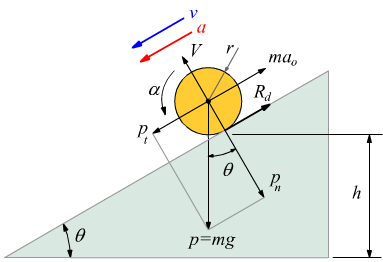
\includegraphics[width = 0.45 \textwidth]{image/motoRototraslatorioPianoIncl.png}
    \caption{Moto rototraslazione di un cilindro pieno su piano inclinato }
    \label{fig:motoRotoTras}
\end{figure}

In questo esercizio, vorremmo capire come è influenzata l'accelerazione di un corpo che rotola giù per un piano inclinato.
Per arrivare alla soluzione del problema dobbiamo utilizzare la legge fondamentale della dinamica rotazionale \ref{equazioneFondamentaleDinamicaRotazionale}.

\begin{equation*}
    M = I\alpha
\end{equation*}

L'equazione rotatoria del cilindro, o disco, pieno è conveniente scriverla rispetto al punto fermo di rotazione \footnote{punto di appoggio del cilindro sul piano inclinato}, e non rispetto al suo baricentro, perché il cilindro sta ruotando rispetto al punto fermo e non rispetto al mozzo il quale si muove durante il rotolamento del cilindro.

Questo punto fermo, ovvero dove avviene la rotazione, è chiamato punto di \textit{istantanea rotazione}.

Il punto di istantanea rotazione continua a cambiare istantaneamente, perché se ruotasse attorno a quel punto dovrebbe entrare nel piano inclinato.

\paragraph{}
La velocità nel punto di istantanea rotazione è:
\begin{equation*}
    V_i = \omega r = \omega * 0  = 0
\end{equation*}

La velocità del baricentro:
\begin{equation*}
    V_b = \omega r
\end{equation*}

Mentre la velocità nel punto più veloce\footnote{diametralmente opposto al punto fermo e viaggia ad una velocità doppia rispetto alla velocità del baricentro} è:
\begin{equation*}
    V_a = 2\omega r = 2V_b
\end{equation*}

Inoltre non mi conviene scrivere l'equazione rispetto al baricentro perché dovrei scrivere il momento di tutte le forze applicate nel baricentro del cilindro: 

\begin{itemize}
    \item la forza peso, però essendo applicato proprio nel baricentro essa ha momento nullo,
    \item la forza normale, $V$,
    \item la forza di attrito, $R_d$,  che agisce sulla ruota ed è proprio questa la forza responsabile del rotolamento.
\end{itemize}

Dopo aver stabilito che non è conveniente scrivere l'equazione rispetto al baricentro, ritorniamo sui nostri passi e iniziamo a scrivere l'equazione rispetto al punto di istantanea rotazione.
I momenti della forze applicate a questo punto sono: 

\begin{itemize}
    \item la forza normale, $V$, è nulla perché il suo momento è zero essendo applicato al punto fermo,
    \item la forza di attrito, $R_d$, come la forza normale, è nulla perché il suo momento è zero essendo applicata al punto fermo,
    \item la forza peso, ed è l'unica che genera momento nel punto di istantanea.
\end{itemize}

Dunque il momento meccanico della forza peso rispetto al punto di rotazione ($M = \vec{r}\times \vec{F}$, braccio prodotto vettoriale forza applicata) è:
\begin{equation*}
   M = \vec{r} \times m\vec{g} = r\sin\theta mg
\end{equation*}

Momento di inerzia rispetto al punto di rotazione, dato dalle principali formule dei momenti di inerzia è la seguente:
\begin{equation*}
   \frac{3}{2}Mr^2
\end{equation*}

\subsubsection{Teorema di Huygens-Steiner }
Per ricavare questo momento di inerzia, oltre che con i valori tabulati dei principali momenti di inerzia, si può applicare il teorema di Huygens-Steiner.

Il teorema afferma che: il momento di inerzia rispetto ad un punto di rotazione, è uguale al momento di inerzia nel baricentro più la massa $M$ per la distanza al quadrato rispetto al punto della rotazione dal baricentro, che in questo caso corrisponde al raggio al quadrato.

\begin{equation*}
   I_0 = \frac{1}{2}MR^2 + MR^2 = \frac{3}{2}MR^2
\end{equation*}

e vediamo che corrisponde al valore della Formula \ref{discoAsseBordo}

\paragraph{}
Accelerazione del momento angolare $\alpha$:\\
l'ultimo ingrediente che ci serve per utilizzare la legge fondamentale, $M = I\alpha$, è calcolare l'accelerazione del momento angolare:

\begin{equation*}
   \alpha = \frac{a_b}{r}\footnote{$a_b$ = accelerazione del baricentro}
\end{equation*}

per trovare l'accelerazione del baricentro basta derivare della velocità del baricentro, $v_b$:

\begin{equation*}
   v_b = \omega r
\end{equation*}
\begin{equation*}
   a_b = \alpha r
\end{equation*}


Ora possiamo scrivere l'equazione del cilindro in discesa sul piano inclinato grazie alla legge fondamentale della dinamica rotazionale \ref{equazioneFondamentaleDinamicaRotazionale}:

\begin{equation*}
    r\sin\theta mg = \frac{3}{2}mr^2\frac{a_b}{r}
\end{equation*}
\begin{equation}
    mg\sin\theta  = \frac{3}{2}mra_b
\end{equation}

dunque l'accelerazione del baricentro è:

\begin{equation*}
    a_b = \frac{2}{3}\biggl(\frac{mg\sin\theta}{m}\biggl)
\end{equation*}
\begin{equation}
    a_b = \frac{2}{3}g\sin\theta
\end{equation}

In questa formula sono da notare due cose: 

\begin{itemize}
    \item $\frac{2}{3}$, tale numero indica che sta rotolando più lentamente, per colpa dell'attrito il quale in questo esempio non lavora ma modifica l'accelerazione, di $\frac{2}{3}$ della accelerazione rispetto ad un oggetto che scivola senza attrito.
    \item la massa non influenza l'accelerazione, infatti si semplifica.
\end{itemize}

Se volessimo trovare il tempo o la velocità finale possiamo utilizzare la formula del moto rettilinea uniformemente accelerato infatti la formula \ref{img:motorettuniformementeacc} diventa:

\begin{equation}
    \frac{h}{\sin{\theta}} = \frac{1}{2}\frac{2}{3}g\sin{\theta}t^2
\end{equation}

dunque il tempo impiegato per scendere è:
\begin{equation}
    t = \sqrt{\frac{3h}{g\sin{\theta}^2}}
\end{equation}

la velocità finale:
\begin{equation}
   v_f = \sqrt{\frac{4}{3}gh} < \sqrt{2gh}\footnote{velocità finale di un corpo che scivola senza attrito}
\end{equation}

\subsubsection{}
Se fosse una sfera piena, il suo momento d'inerzia baricentrale sarebbe:
\begin{equation*}
    I = \frac{2}{5}MR^2
\end{equation*}

applicando il teorema di Huygens-Steiner:
\begin{equation*}
    I = \frac{2}{5}Mr^2 + Mr^2 = \frac{7}{5}Mr^2
\end{equation*}

e dunque l'accelerazione della sfera che scende da un piano inclinato è:
\begin{equation*}
   r\sin\theta mg = \frac{7}{5}mr^2\frac{a_b}{r}
\end{equation*}
\begin{equation}
   a_b = \frac{5}{7}(g\sin\theta)
\end{equation}

Come notiamo la sfera piena avrà un'accelerazione inferiore rispetto ad un oggetto che pattina sul piano inclinato, ma la sua accelerazione è superiore rispetto al cilindro pieno, e questo, di fatto, sta a significare che una biglia su un piano inclinato arriverà prima del cilindro alla base. Di fatto però la biglia si fermerà prima rispetto al cilindro quando inizieranno a viaggiare su un piano piatto.

Questo è dovuto al fatto che il cilindro è più inerte \footnote{cerca di mantenere il suo moto rettilineo uniforme, ovvero la sua velocità} rispetto ad una sfera la quale è più efficiente dal punto di vista inerziale\footnote{si impiega meno forza per partire} del disco. Ciò e dato dal fatto che la massa è più concentrata nel baricentro, mentre nel disco è distribuita in maniera più uniforme.
\paragraph{}
Dato questo paragone si può intuire che un cilindro cavo impiegherebbe ancora più tempo per arriverebbe alla base del piano inclinato, infatti esso minimizza l'accelerazione perché svolgendo i calcoli si avrà la metà, $\frac{1}{2}$, dell'accelerazione di un oggetto che pattina senza attrito.

\subsection{Assi principali di inerzia}

\begin{figure}[H]
    \centering
    \begin{minipage}[c]{0.4\textwidth}
    \centering
    \def\ang{-20}
    \begin{tikzpicture}[rotate=\ang, scale = 1]
      \def\h{0.9}   % length z axis
      \def\L{3.0}   % length rod
      \def\R{1.9}   % circle radius
      \def\r{1.4}   % mass radius (inner sep)
      \coordinate (O) at (0,0);
      \coordinate (L) at (-\R/2,0);
      \coordinate (R) at ( \R/2,0);
      \draw[->](0.18,-\h) -- (-0.465,\h) coordinate (T);
      \pic[xscale=1] at (-0.4,0.7*\h) {rotarr};
      \node[below=1,right=1] at (W3) {$\omega$};
      \draw[line width=1.8,red!25!black] (L) -- (R);
      \node[mass,circle,inner sep=\r,scale=0.8] (L') at (L) {$m_1$};
      \node[mass,circle,inner sep=\r,scale=0.8] (R') at (R) {$m_2$};
      \draw[<->] (L)++(0,-0.2*\R) --++ ( \R/2,0) node[midway,below=-1] {$r_1$}; %\frac{r}{2}
      \draw[<->] (R)++(0,-0.2*\R) --++ (-\R/2,0) node[midway,below=-1] {$r_2$};
      
      \draw[->,myblue](\R/2,0) -- (\R/2,1) node[above,right]{$\vec{l_2}$};
      \draw[->,myblue](-\R/2,0) -- (-\R/2,1) node[above,left]{$\vec{l_1}$};
      \draw[->,myblue](-0.18,0) -- (-0.18,2) node[above,left]{$\vec{L}$};
    
    
    \end{tikzpicture}
    \caption{$\vec{L}$ non proporzionale a $\vec{\omega}$}
    \label{fig:nonProporzionale}
    \end{minipage}
    \hspace{0.1mm}
    \begin{minipage}[c]{0.4\textwidth}
    \centering
    \begin{tikzpicture}[scale = 1]
      \def\h{0.9}   % length z axis
      \def\L{3.0}   % length rod
      \def\R{1.9}   % circle radius
      \def\r{1.4}   % mass radius (inner sep)
      \coordinate (O) at (0,0);
      \coordinate (L) at (-\R/2,0);
      \coordinate (R) at ( \R/2,0);
      \draw[->] (0,-\h) -- (0,\h) coordinate (T);
      \pic[xscale=1] at (0,0.7*\h) {rotarr};
      \node[below=1,right=1] at (W3) {$\omega$};
      \draw[line width=1.8,red!25!black] (L) -- (R);
      \node[mass,circle,inner sep=\r,scale=0.8] (L') at (L) {$m$};
      \node[mass,circle,inner sep=\r,scale=0.8] (R') at (R) {$m$};
      \draw[<->] (L)++(0,-0.2*\R) --++ ( \R/2,0) node[midway,below=-1] {$r$}; %\frac{r}{2}
      \draw[<->] (R)++(0,-0.2*\R) --++ (-\R/2,0) node[midway,below=-1] {$r$};
      
      \draw[->,myblue](\R/2,0) -- (\R/2,1) node[above,right]{$\vec{l_2}$};
      \draw[->,myblue](-\R/2,0) -- (-\R/2,1) node[above,left]{$\vec{l_1}$};
      \draw[->,myblue](0,0) -- (0,2) node[above,left]{$\vec{L}$};
    \end{tikzpicture}
    \caption{Caso simmetria rispetto a $\vec{\omega}$}
    \label{fig:casoSimmetrico}
    \end{minipage}
\end{figure}

Il momento d'inerzia è un vettore che sembra proporzionale al vettore velocità angolare, in realtà vedremo che non è così.
Si prenda come esempio la Figura \ref{fig:nonProporzionale}.

In generale la relazione:

\begin{equation*}
    \vec{L} \neq I\vec{\omega}
\end{equation*}


Calcoliamo il momento angolare di 2 masse puntiformi, e per calcolarlo, basta sommare tutti i momenti angolari: $\vec{r}\times\vec{p}\,\footnote{$\vec{p} = mv$}$.

Si nota ad occhio che il momento angolare totale non è proporzionale rispetto a $\omega$, infatti $I$ non è un semplice scalare ma è un tensore il quale trasforma il vettore $\vec{\omega}$ in un nuovo vettore: $\vec{L}$.
In questo caso $\vec{L}$ è diverso sia in modulo, in direzione e verso rispetto ad $\vec{\omega}$.
\paragraph{}

In figura \ref{fig:casoSimmetrico} viene rappresentatala un caso simile ma con molte simmetrie. In questo caso la relazione $\vec{L} = I\vec{\omega}$ vale in quanto cambia solo il modulo.
Ma momento inerziale intermedio dei tre principali è instabile.


\newpage
\subsection{Conservazione dell'energia meccanica del moto rototraslatorio}
La formula della conservazione dell'energia è ancora valida, ma bisogna aggiungere anche il moto rotatorio perché difatti è energia cinetica, ed è data dalla seguente formula:

\begin{equation*}
    E_{tot} = E_p + E_c
\end{equation*}

\begin{equation}
    E_{tot} = mgh + \frac{1}{2}mv_b^2 + \frac{1}{2}I_b\omega^2
\end{equation}

Riprendendo l'esercizio del piano inclinato svolto a Pagina \pageref{fig:motoRotoTras} possiamo calcolare la velocità finale anche grazie all'energia. Vediamo come:

Sappiamo che l'energia potenziale alla sommità del piano inclinato deve essere uguale all'energia cinetica alla base del piano inclinato $E_p + 0 = 0 + E_c$:
\begin{equation*}
    mgh =  \frac{1}{2}mv_b^2 + \frac{1}{2}I_b\omega^2 = \frac{1}{2}mv_b^2 + \frac{1}{4}mv_b^2 = \frac{3}{4}mv_b^2
\end{equation*}

Dunque la velocità finale è:
\begin{equation}
    v_b = \sqrt{\frac{4}{3}gh}
\end{equation}

che è uguale, ovviamente, a quella trovata con il moto rettilineo uniformemente accelerato.

Più in generale la velocità finale di un corpo che rotola giù su un piano inclinato è la seguente:

\begin{equation}
    v_f = \sqrt{\frac{2gh}{1+\frac{I}{mr^2}}}
\end{equation}

Notiamo che il modulo della velocità dipende dal momento di inerzia e che un momento di inerzia maggiore comporta una velocità minore. 

\subsection{Conservazione del momento angolare}
Il principio di conservazione del momento angolare stabilisce che, se la somma dei momenti delle forze esterne agenti su un corpo è nulla, allora il momento angolare si conserva e quindi costante. 

\begin{equation*}
    \sum \vec{M}_{est} = \sum \frac{\Delta \vec{L}}{\Delta t}
\end{equation*}
dove $\vec{M}_{est}$ e $\vec{L}$ sono definiti nello stesso punto 
\begin{equation*}
    \Delta t\vec{M}_{est} = \Delta\vec{L}
\end{equation*}

ma se $\vec{M_{est}} = 0 $ allora:
\begin{equation*}
    \Delta\vec{L} =  \vec{L}_f -  \vec{L}_i
\end{equation*}

e dunque:
\begin{equation}
   \sum \vec{M}_{est} = 0 \rightarrow  \vec{L}_i = \vec{L}_f 
\end{equation}

Questa legge è l’equivalente rotazionale del principio di conservazione della quantità di moto. 

\paragraph{}
\e possibile estendere il discorso per un sistema di punti: i momenti delle forze interne si elidono a vicenda, per il terzo principio della dinamica, dunque il momento delle forze è dato solo dalla somma dei momenti meccanici esterni. 
Dunque il momento angolare totale si conserva se, come prima, $\sum \vec{M}_{est}  = 0$:

\begin{equation}
    \sum \vec{M}_{est}  = 0 \rightarrow \vec{L}_{tot,i} = \vec{L}_{tot,f}
\end{equation}

\section{La forza di Coriolis}
Nei sistemi di riferimento rotanti può comparire un’altra forza apparente: la forza di Coriolis, dal nome dello scienziato francese che la studiò nel XIX secolo. 
Questa forza:

\begin{itemize}
    \item agisce sugli oggetti in moto rispetto al sistema rotante,
    \item è perpendicolare alla velocità dell’oggetto e all’asse di rotazione.
\end{itemize}

Un oggetto libero, che rispetto a un sistema di riferimento inerziale si muove di moto rettilineo uniforme, Figura \ref{fig:sistemaInerziale}, rispetto a un sistema rotante descrive una traiettoria curvilinea, Figura \ref{fig:sistemaNonInerziale}, a causa della forza di Coriolis.

La forza di Coriolis è direttamente proporzionale alla velocità dell’oggetto e fa deviare
l'oggetto verso destra se il sistema di riferimento ruota in senso antiorario, verso sinistra se il sistema ruota in senso orario.

\def\ang{-20}
\def\R{2}       % disk radius
\def\r{0.1}     % mass radius
\def\v{0.35*\R} % mass velocity
\def\x{0.48}    % mass position (fraction of \R)
\def\ang{50}    % angle displacement
\begin{figure}[H]
    \centering
    \begin{minipage}[c]{0.4\textwidth}
    \centering
    \begin{tikzpicture}
      \coordinate (O) at (0,0);
      \coordinate (T) at (0,\r);
      \coordinate (M) at (90:0.45*\R);
      \coordinate (S) at (-145:1.6*\R);
      \coordinate (B) at (90+\x*\ang:0.88*\R);
      
      % DISK & DOTS
      \draw[disk] (O) circle(\R);
      \fill[myred!20] (90:0.88*\R) circle(0.05*\R);
      \fill[myred] (90+\x*\ang:0.88*\R) circle(0.05*\R);
      \fill[myred!20] (90+\ang:0.88*\R) circle(0.05*\R);
      \draw[xcol,->] (92:0.88*\R) arc(92:88+\ang:0.88*\R);
      
      % MASS
      \draw[<->,black!25,line width=0.9]
        (0,0.35*\R) |-++ (0.35*\R,-0.35*\R);
      \draw[xcol] (O) --++ (90:1.1*\R);
      \draw[vvec] (M) --++ (90:\v) node[below right] {$\vb{v}$};
      \draw[mass] (M) circle(\r) node[right=1] {$m$};
      \draw[->] (10:1.1*\R) arc(10:35:1.1*\R) node[left=2,above=0] {$\omega$};
      
      % AXIS
      \node[left=2] at (S) {S};
      \draw[<->,line width=0.9]
        (S)++(0,0.38*\R) node[left,scale=0.9] {$y$} |-++
             (0.35*\R,-0.35*\R) node[below right=-3,scale=0.9] {$x$};
      
      % AXIS S'
      \draw[<->,line width=0.9]
        (90+\x*\ang:0.35*\R) node[below left=-2,scale=0.9] {$y'$} -- (0,0) --
        (\x*\ang:0.35*\R) node[above=3,right=-2,scale=0.9] {$x'$};
      \node[below=1] at (O) {A};
      \node[right=1,below=1] at (B) {B};
    \end{tikzpicture}
    \caption{Sistema inerziale}
    \label{fig:sistemaInerziale}
    \end{minipage}
    \hspace{5mm}
    \begin{minipage}[c]{0.4\textwidth}
    \centering
    \begin{tikzpicture}
      \def\v{0.40*\R}        % mass velocity
      \def\vv{2.0}           % velocity for plot
      \def\FC{0.30*\R}       % Coriolis force
      \def\om{180/pi}        % angular frequency omega
      \def\tmax{1.10}        % maximum t
      \def\xt{0.98*\x*\tmax} % mass position
      \coordinate (T) at (0,\r);
      \coordinate (S) at (-145-\ang:1.6*\R);
      \coordinate (M) at ({\vv*\xt*sin(\om*\xt)},{\vv*\xt*cos(\om*\xt)});
      \coordinate (V) at ({\v*sin(\om*\xt)+\v*\xt*cos(\om*\xt)},{\v*cos(\om*\xt)-\v*\xt*sin(\om*\xt)});
      \coordinate (F) at ({\FC*cos(\om*\xt)-\FC*\xt*sin(\om*\xt)},{-\FC*sin(\om*\xt)-\FC*\xt*cos(\om*\xt)});
      
      % DISK & DOTS
      \draw[disk] (0,0) circle(\R);
      \fill[myred] (90:0.88*\R) circle(0.05*\R);
      
      % AXIS
      \draw[xcol,dashed] (0,0) --++ (90:1.1*\R);
      \node[below left=-1] at (0,0) {S$'$};
      \draw[<->,line width=0.9]
        (0,0.35*\R) node[left,scale=0.9] {$y'$} |-++
        (0.35*\R,-0.35*\R) node[below right=-3.5,scale=0.9] {$x'$};
      
      % MASS
      \draw[xcol,samples=50,smooth,variable=\t,domain=0:\tmax]
        plot({\vv*\t*sin(\om*\t)},{\vv*\t*cos(\om*\t)});
      %\fill[myred] (90-\ang:0.88*\R) circle(0.05); % check
      \draw[vvec] (M) --++ (V) node[above=3,left=0] {$\vb{v}$};
      \draw[force] (M) --++ (F) node[right=-1] {$\vb{F}_\mathrm{Cor}$};
      \draw[mass] (M) circle(\r) node[left=4,above=2] {$m$};
      
      % AXIS
      \node[left=2] at (S) {S};
      \draw[<->,black!25,line width=0.9]
        (-145:1.6*\R)++(0,0.38*\R) node[left,scale=0.9] {$y$} |-++
                       (0.35*\R,-0.35*\R) node[below right=-3,scale=0.9] {$x$};
      \draw[<->,line width=0.9]
        (S)++(90-\ang:0.38*\R) node[left=3,scale=0.9] {$y$} --++ (-90-\ang:0.38*\R) --++
             (-\ang:0.38*\R) node[below right=-3,scale=0.9] {$x$};
      \draw[->] (-165:1.55*\R) arc(-150:-210:0.6*\R) node[midway,left=0] {$\omega$};
      
    \end{tikzpicture}
    \caption{Sistema non inerziale}
    \label{fig:sistemaNonInerziale}
    \end{minipage}
\end{figure} 

\paragraph{}
La forza di Coriolis è anche responsabile di vari fenomeni che avvengono su scala planetaria e che riguardano il movimento delle masse d’aria e delle correnti oceaniche.
\paragraph{}
A causa del suo moto di rotazione e di rivoluzione, come abbiamo visto, la Terra non è un sistema di riferimento inerziale; tuttavia, poiché le accelerazioni centripete legate a questi moti sono centinaia di volte più piccole dell'accelerazione di gravità, nella maggior parte dei casi gli effetti di non inerzialità sono ininfluenti ed è possibile considerare, con ottima approssimazione, un laboratorio terrestre come un sistema di riferimento inerziale. 

Ci sono però delle situazioni in cui le conseguenze del moto di rotazione della Terra e delle forze apparenti da esso generate sono avvertibili. La forza di Coriolis in particolare, fa sì che un oggetto che si muove verso nord sulla superficie terrestre venga deviato verso est o verso ovest, a seconda che si trovi nell'emisfero boreale o nell'emisfero australe, come mostrato in Figura \ref{fig:coriolisTerra}.

\begin{figure}[tb]
    \centering
    \contourlength{0.7pt}
    \begin{tikzpicture}[scale = 1.5]
      \def\E{1.2}
      \coordinate (O) at (0,0);
      
      % EARTH
      \draw[dashed,rotate=-11] (0,-1.3*\E) -- (0,1.45*\E);
      \fill[blue!70!black!70] (0,0) circle (1.2);
      \draw[very thin,ball color=blue!70!black!40,fill opacity=0.2] (0,0) circle (\E);
      \begin{scope}[rotate=-11]
        \draw[-{Latex[length=3,width=2,flex'=1]}] (0,1.22*\E)++(120:{0.2*\E} and 0.1*\E) arc(120:430:{0.2*\E} and 0.1*\E);
        \clip (0,0) circle (\E);
        \fill[white] (0,\E) ellipse ({0.6*\E} and {0.15*\E});
        \fill[white] (0,-\E) ellipse ({0.8*\E} and {0.08*\E});
        \fill[green!70!black!60,rotate=-30] (160:1.1*\E) ellipse ({0.2*\E} and {0.8*\E});
        \fill[green!70!black!60,rotate=40] (-10:1.14*\E) ellipse ({0.2*\E} and {0.9*\E});
        \fill[green!60!black!60,very thick,rotate=-20] % Australia
          (230:0.86*\E) ellipse ({0.25*\E} and {0.18*\E});
        \draw[dashed] (-\E,0) to[out=-20,in=-160] (\E,0);
        
        % CORIOLIS
        \draw[myred,mydashed,very thin] (0,-0.1*\E) coordinate (NS) --++ (0, 0.70*\E) coordinate (NN);
        \draw[myred,mydashed,very thin] (0,-0.3*\E) coordinate (SN) --++ (0,-0.60*\E) coordinate (SS);
        \draw[myred,mydashed,very thin] (-0.4*\E,0.32*\E) coordinate (NW) to[out=-20,in=-160]++ (0.8*\E,0) coordinate (NE);
        \draw[myred,mydashed,very thin] (-0.4*\E,-0.53*\E) coordinate (SW) to[out=-20,in=-160]++ (0.8*\E,0) coordinate (SE);
        \draw[myarr,red] (NN) to[out=-90,in=  50]++ (-110:0.35*\E); % northern hemisphere
        \draw[myarr,red] (NS) to[out= 90,in=-120]++ (  70:0.35*\E);
        \draw[myarr,red] (SN) to[out=-90,in= 130]++ ( -65:0.30*\E); % southern hemisphere
        \draw[myarr,red] (SS) to[out= 90,in= -60]++ ( 110:0.30*\E);
        \draw[myarr,red] (NE) to[out=200,in= -40]++ (170:0.38*\E); % northern hemisphere
        \draw[myarr,red] (NW) to[out=-20,in= 140]++ (-30:0.42*\E);
        \draw[myarr,red] (SE) to[out=200,in=  40]++ (210:0.42*\E); % southern hemisphere
        \draw[myarr,red] (SW) to[out=-20,in=-140]++ ( 10:0.38*\E);
      \end{scope}
      
      \node at (108-11:1.2*\E) {N};
      \node at (180-11:1.2*\E) {W};
      \node at (   -11:1.2*\E) {E};
      \node at (-98-11:1.2*\E) {S};
      
    \end{tikzpicture}
    \caption{Forza di Coriolis nei due emisferi}
    \label{fig:coriolisTerra}
\end{figure}

\newpage 
\ 
\newpage

\part{Elettromagnetismo}


\chapter{Campo Elettrico}

Come la massa, la carica elettrica è una proprietà intrinseca delle particelle. A
differenza della massa la carica elettrica si presenta in due tipi distinti:

\begin{itemize}
    \item Cariche positive
    \item Cariche negative
\end{itemize}

L’unità di misura della carica elettrica nel SI è il coulomb ($C$).

\section{Carica elettrica fondamentale}
Gli esperimenti hanno mostrato che il valore della carica elettrica di un protone
è esattamente uguale a quella di un elettrone: un protone ha carica $e^+$ mentre un
elettrone ha carica $e^-$.

La costante $e$ è definita \textbf{carica elettrica fondamentale} e vale:

\begin{equation}
    e = 1,602176634 \cdot 10^{-19} \quad[C]
\end{equation}

Visto che il numero di protoni ed elettroni in un atomo è lo stesso, la somma
algebrica delle cariche positive dei protoni nel nucleo e di quelle negative degli
elettroni è zero. Di conseguenza,
gli atomi sono elettricamente neutri perché la loro carica totale è nulla.
\paragraph{}
La carica di un elettrone o di un protone è il più piccolo valore di carica libera che
sia mai stato misurato. Poiché, come vedremo, la carica totale $Q$ di un corpo può
essere cambiata aumentando o diminuendo il numero di elettroni, questo vuol
dire che:

ogni carica $Q$ è un multiplo intero di $e$, ovvero $Q = ne\,,\,n \in \mathbb{N}$.

\paragraph{}
Generalmente sono gli elettroni a
essere trasferiti:

\begin{itemize}
    \item i corpi che guadagnano elettroni acquistano un eccesso di carica negativa e diventano carichi negativamente;
    \item i corpi che perdono elettroni rimangono con un eccesso di carica positiva e diventano carichi positivamente.
\end{itemize}


\section{Forza elettrostatica}

\def\a{2.5}
\def\R{0.33}
\def\F{1.8}
\begin{figure}[H]
    \centering
    \begin{tikzpicture}[scale = 1.3]
      \coordinate (L) at (-\a,0);
      \coordinate (R) at (+\a,0);
        
      % FORCES
      \draw[force] (L) --++ (+\F,0) node[above left] {$\mathbf{F}_{12}$};
      \draw[force] (R) --++ (-\F,0) node[above right] {$\mathbf{F}_{21}$};
      
      % CHARGES
      \draw[charge+] (L) circle (\R) node[scale=1.2] {$+$};
      \draw[charge-] (R) circle (\R) node[scale=1.2] {$-$};
      \draw[<->]     (L)++(\R,-1.1*\R) --++ (2*\a-2*\R,0) node[midway,below] {r};
      \node[above] at (-\a,\R) {$q_1$};
      \node[above] at (+\a,\R) {$q_2$};
      
    \end{tikzpicture}
    \caption{Forza elettrostatica}
    \label{fig:forzaElettrica}
\end{figure}

Due cariche esercitano una forza reciproca fra loro e questa forza sarà:
\begin{itemize}
    \item attrattiva se le due cariche sono opposte;
    \item repulsiva se le due cariche hanno lo stesso segno, positivo o negativo.
\end{itemize}




\subsection{Legge di Coulomb}
Questa legge permette di calcolare la forza elettrostatica esercitata tra due cariche nel vuoto:

\begin{equation}
    F = K_e\frac{|q_1||q_2|}{r^2} \qquad[N]
\end{equation}

tale formula permette di calcolare l'intensità della forza elettrostatica dalla prima carica sulla seconda e viceversa.
\paragraph{}
Il simbolo $K_e$, o costante di Coulomb, viene determinato sperimentalmente e risulta essere circa:

\begin{equation}
    K_e \simeq 8,99\cdot10^{9}\qquad \biggl[\frac{N\,m^2}{C^2}\biggl]
\end{equation}

\paragraph{}
Questa legge però risulta limitante, infatti solitamente un corpo è sempre immerso in un materiale, come ad esempio l'aria.

Proprio per questo motivo si è introdotta una nuova costante $\epsilon_0$ chiamata costante dielettrica nel vuoto la quale vale circa: 
 \begin{equation}
    \varepsilon_0 \simeq 8.854\cdot10^{9}\qquad \biggl[\frac{C^2}{N\,m^2}\biggl]
\end{equation}

Dunque $K_e$ risulterà essere:
 \begin{equation}
    K_e = \frac{1}{4\pi\varepsilon_0}
    \label{keFrazioneEpsilon}
\end{equation}

e la legge di Coulomb quindi:

\begin{equation}
    F = \frac{1}{4\pi\varepsilon_0}\frac{|q_1||q_2|}{r^2}
\end{equation}

\paragraph{}
Guardando la Figura \ref{fig:forzaElettrica}, se scegliamo come riferimento valori i positivi per forze verso destra e valori negativi per forze verso sinistra, applicando la legge di Coulomb risulterà che:

\begin{itemize}
    \item la carica $q_1$ avrà una forza positiva, $+F$ diretta verso $q_2$
    \item la carica $q_2$ avrà una forza negativa, $-F$ diretta verso $q_1$
\end{itemize}


\subsection{Analogie e differenze con la legge di gravitazione universale}
La forza elettrica e la forza gravitazionale hanno molte analogie e alcune differenze. Partendo dalle due formule, indichiamo con $F_e$ la forza elettrica e con $F_g$ la forza gravitazionale:

\begin{equation*}
    F_e = K_e\frac{|q_1||q_2|}{r^2} \qquad F_g = G\frac{|m_1||m_2|}{r^2}
\end{equation*}

\subsubsection{Analogie:}
\begin{itemize}
    \item dipendono da una costante universale (se consideriamo $F_e$ nel vuoto)
    \item esercitano una forza su una coppia di corpi
    \item esercitano una forza a distanza
    \item sono inversamente proporzionali al quadrato della distanza tra i due corpi che interagiscono
\end{itemize}
\subsubsection{Differenze:}
\begin{itemize}
    \item la forza elettrica sovrasta di venti ordini di grandezza la forza di gravità:
        \begin{equation*}
            K_e \simeq 8,99\cdot10^{9}\qquad \biggl[\frac{N\,m^2}{C^2}\biggl]
        \end{equation*}
        \begin{equation*}
            G \simeq 6,67\cdot10^{-11}\qquad \biggl[\frac{N\,m^2}{Kg^2}\biggl]
        \end{equation*}
    \item la forza gravitazionale è solo attrattiva, la forza di Coulomb può essere attrattiva o repulsiva;
    \item la forza gravitazionale si esercita su qualunque coppia di corpi perché dipende unicamente dalle loro masse, la forza di Coulomb si manifesta solo tra corpi dotati di carica elettrica.
\end{itemize}

Proprio su questo ultimo punto volevo soffermarmi: sulla terra crediamo che la forza di gravità si molto potente.
Questo fatto lo si può spiegare facilmente perché la maggior parte degli oggetti sono neutri e dunque, proprio per questo motivo, la forza elettrica viene completamente oscurata dalla forza di gravità.

\section{Sovrapposizione delle cariche elettriche}
La legge di Coulomb stabilisce come calcolare la forza che una carica puntiforme
esercita su un’altra carica puntiforme. Nella realtà, però, una carica è soggetta
alle forze causate da tutte le cariche che la circondano e per determinare la forza
totale che agisce su una carica bisogna applicare il principio di sovrapposizione:

\begin{equation*}
    \vec{F}_{tot,1} = \vec{F}_{1,2} + \vec{F}_{1,3} + \dots + \vec{F}_{1,n}
\end{equation*}
generalizzando
\begin{equation}
    \vec{F}_{tot,j} = \sum_{i = 1, i\neq j}^n \vec{F}_{j,i}
\end{equation}

\section{Il campo elettrico}

Consideriamo una carica puntiforme $Q_1$
 ferma in un punto: se le avviciniamo una carica puntiforme $Q_2$ , essa risente di una forza data dalla legge di Coulomb. Questo
significa che $Q_1$ interagisce con $Q_2$ e proprio questa forza, come detto in precedenza, è una forza a distanza.
\paragraph{}
Come può esistere un’azione fra le due
cariche senza un mezzo materiale che la trasporti?
Per rispondere a questa domanda si può concludere che non esiste alcuna forza a distanza senza l'intervento di una grandezza fisica che funge da intermediario, ed è proprio qui che si inizia a parlare del concetto di \textit{campo}.
\paragraph{}
Pensiamo alla Terra, essa genera attorno a sé un campo di forze (gravitazionali), e qualunque oggetto dotato di massa che si trova nel suo raggio d'azione, viene attratto verso il suo centro. Non è la Terra, direttamente, che attrae il corpo, ma il suo campo delle forze che agiscono sull'oggetto massivo, determinandone la caduta.

\paragraph{}
Ritornando al capo elettrico, si pensi alla stessa analogia: la carica $Q_1$
 genera un campo elettrico che modifica le proprietà dello
spazio circostante, il quale diventa sede di forze elettriche, Figura \ref{fig:campoElettricoPosNeg}.
Quando la carica $Q_2$  viene posizionata in un punto dello spazio, sente una forza che dipende dal fatto che $Q_1$ ha
modificato le proprietà dello spazio in quel punto. Così $Q_2$
 non interagisce direttamente con $Q_1$.
 ma con il campo elettrico che questa ha generato in quel punto, Figura \ref{fig:campoElettricoAttrRep}.
 
 \def\R{1.8}
\def\NE{8}
\def\NV{4}
\contourlength{1.6pt}
 \begin{figure}[H]
     \centering
     \begin{minipage}[c]{0.4\textwidth}
     \centering
        \begin{tikzpicture}[scale = 1.3]
          \foreach \i [evaluate={\angle=(\i-1)*360/\NE;}] in {1,...,\NE}{
            \draw[EFieldLineArrow={0.6}] (0,0) -- (\angle:\R);
          }
          \draw[charge+] (0,0) circle (7pt) node[black,scale=0.8] {$+Q$};
           
        \end{tikzpicture}
      \end{minipage}
     \hspace{0.1mm}
     \begin{minipage}[c]{0.4\textwidth}
        \centering
        \begin{tikzpicture}[scale = 1.3]
          \foreach \i [evaluate={\angle=(\i-1)*360/\NE;}] in {1,...,\NE}{
            \draw[EFieldLineArrow={0.5}] (\angle:\R) -- (0:0);
          }
          \draw[charge-] (0,0) circle (7pt) node[black,scale=0.8] {$-Q$};
        \end{tikzpicture}
     \end{minipage}
     \caption{Campo elettrico di una particella positiva a sinistra e negativa a destra}
     \label{fig:campoElettricoPosNeg}
 \end{figure}
 
 \subsection{Definizione di campo elettrico}
 
  \begin{figure}[H]
     \centering
     \begin{minipage}[c]{0.4\textwidth}
     \centering
            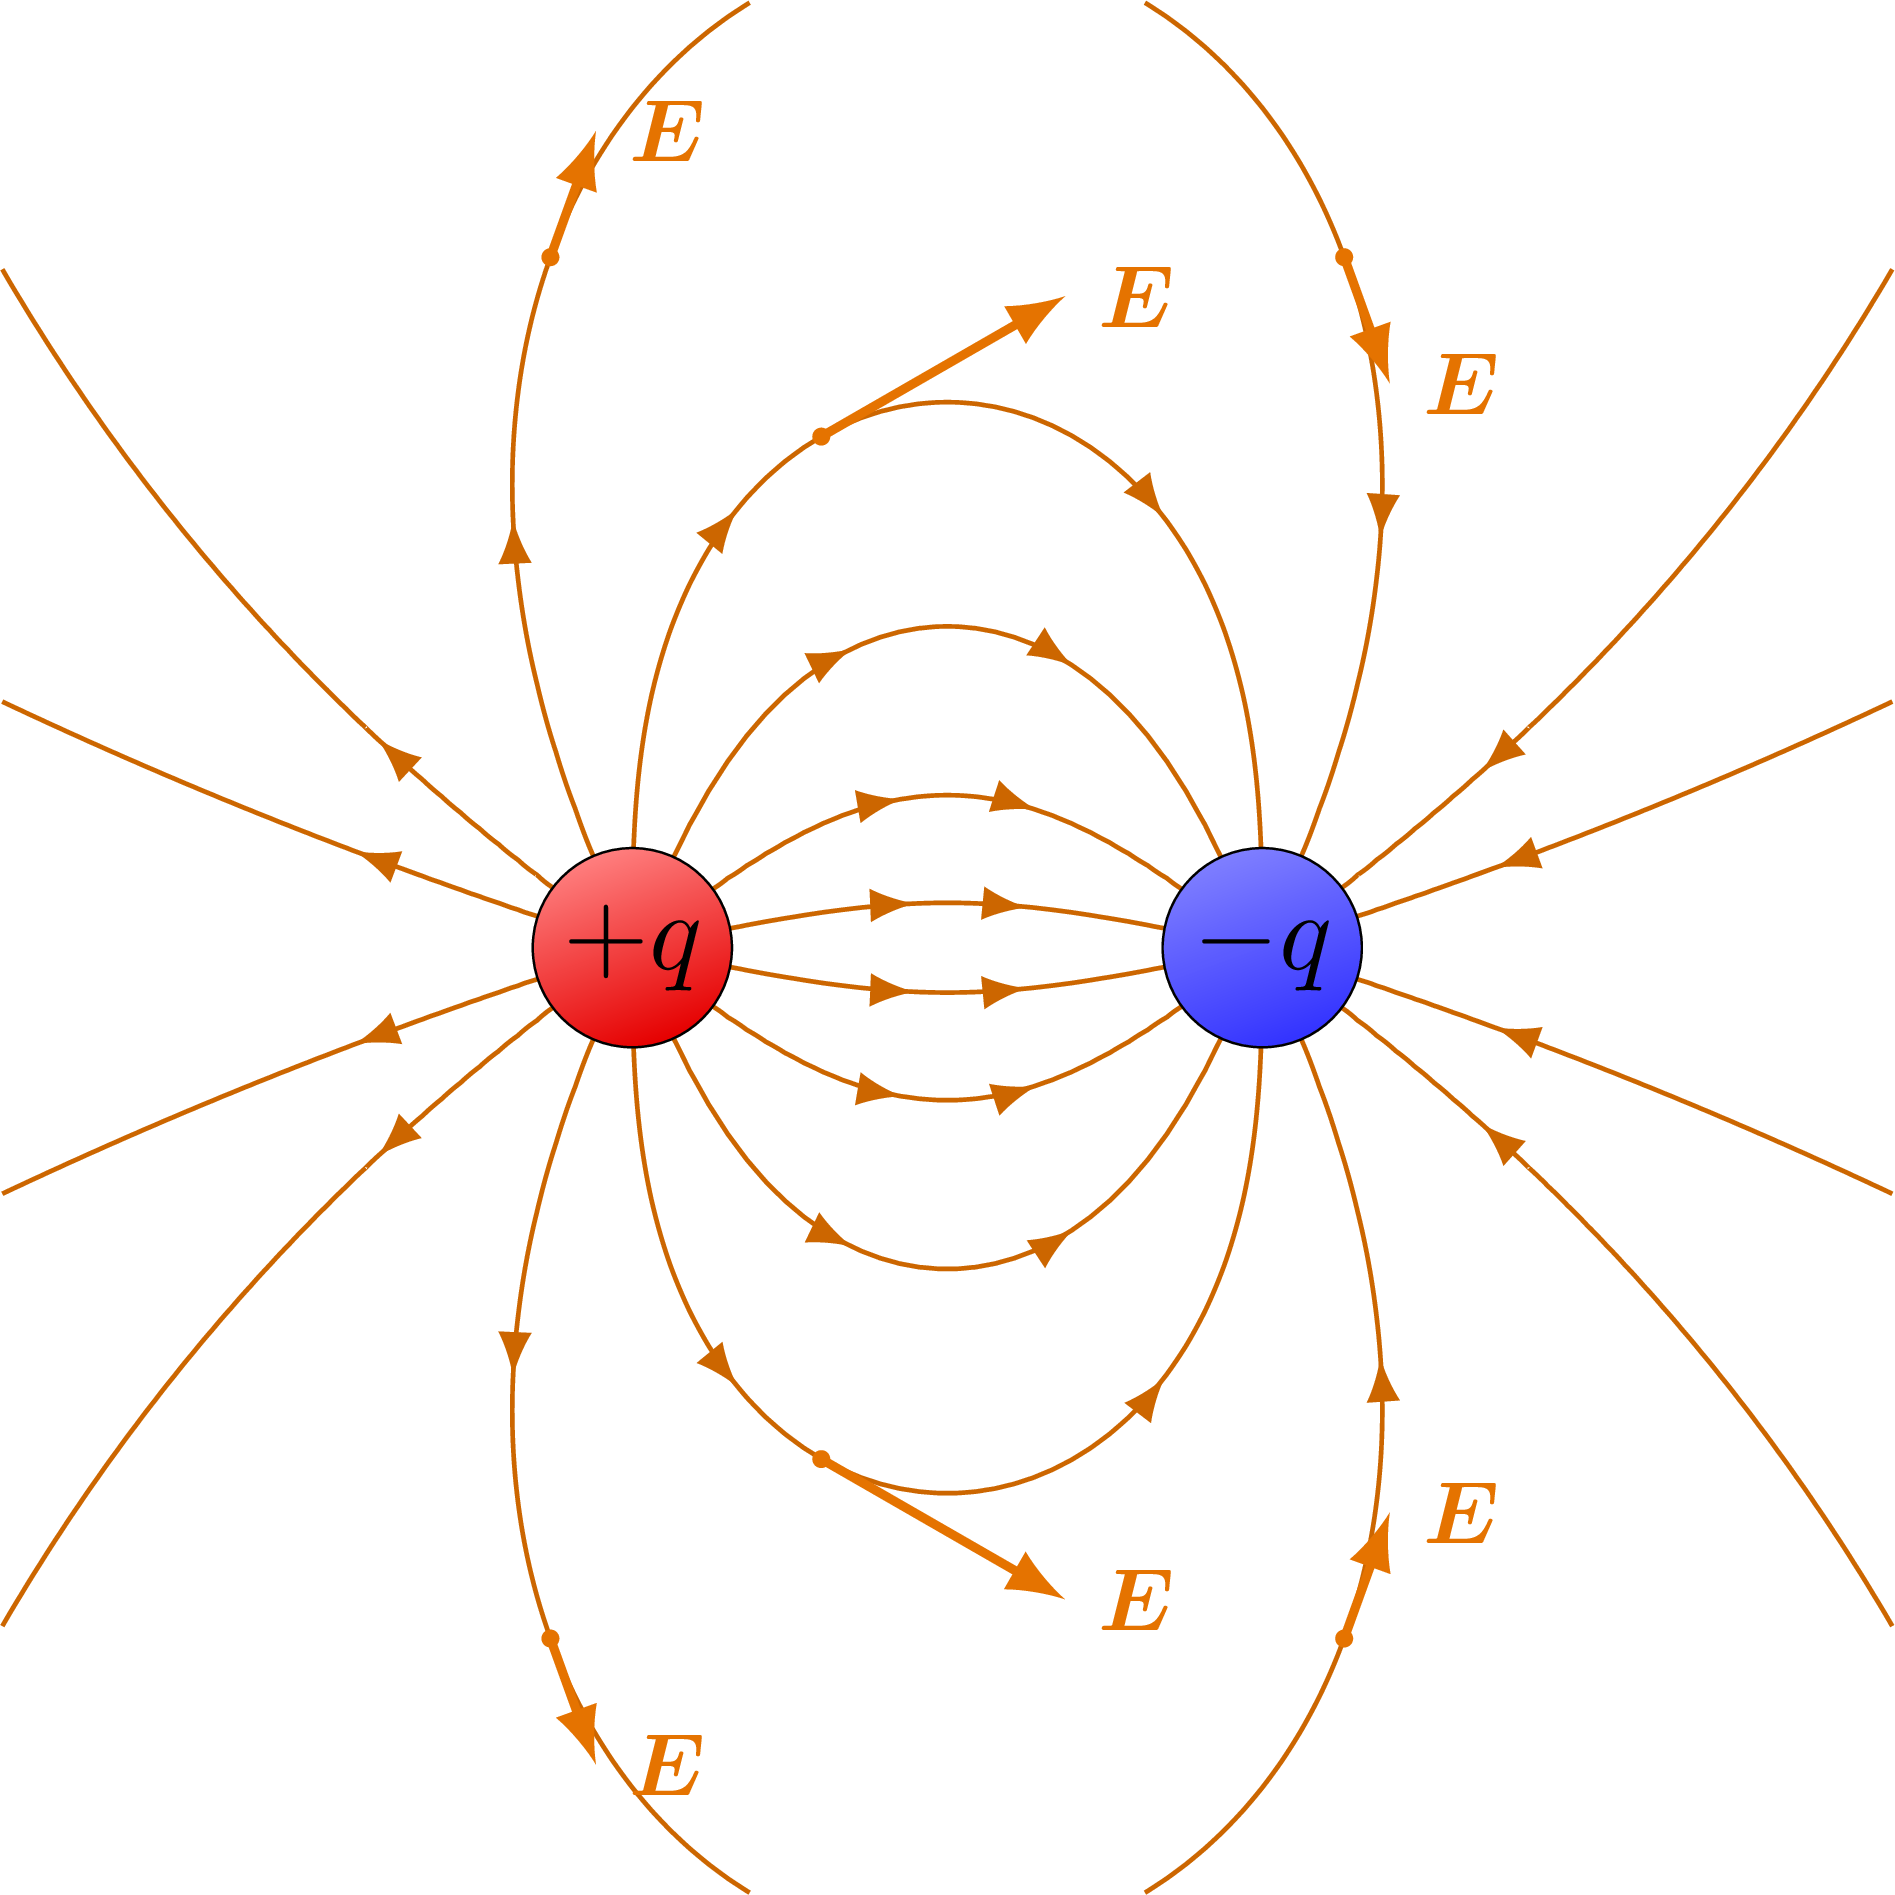
\includegraphics[width = 1\textwidth]{image/interazioneCampiElettrici.png}
      \end{minipage}
     \hspace{0.1mm}
     \begin{minipage}[c]{0.4\textwidth}
        \centering
        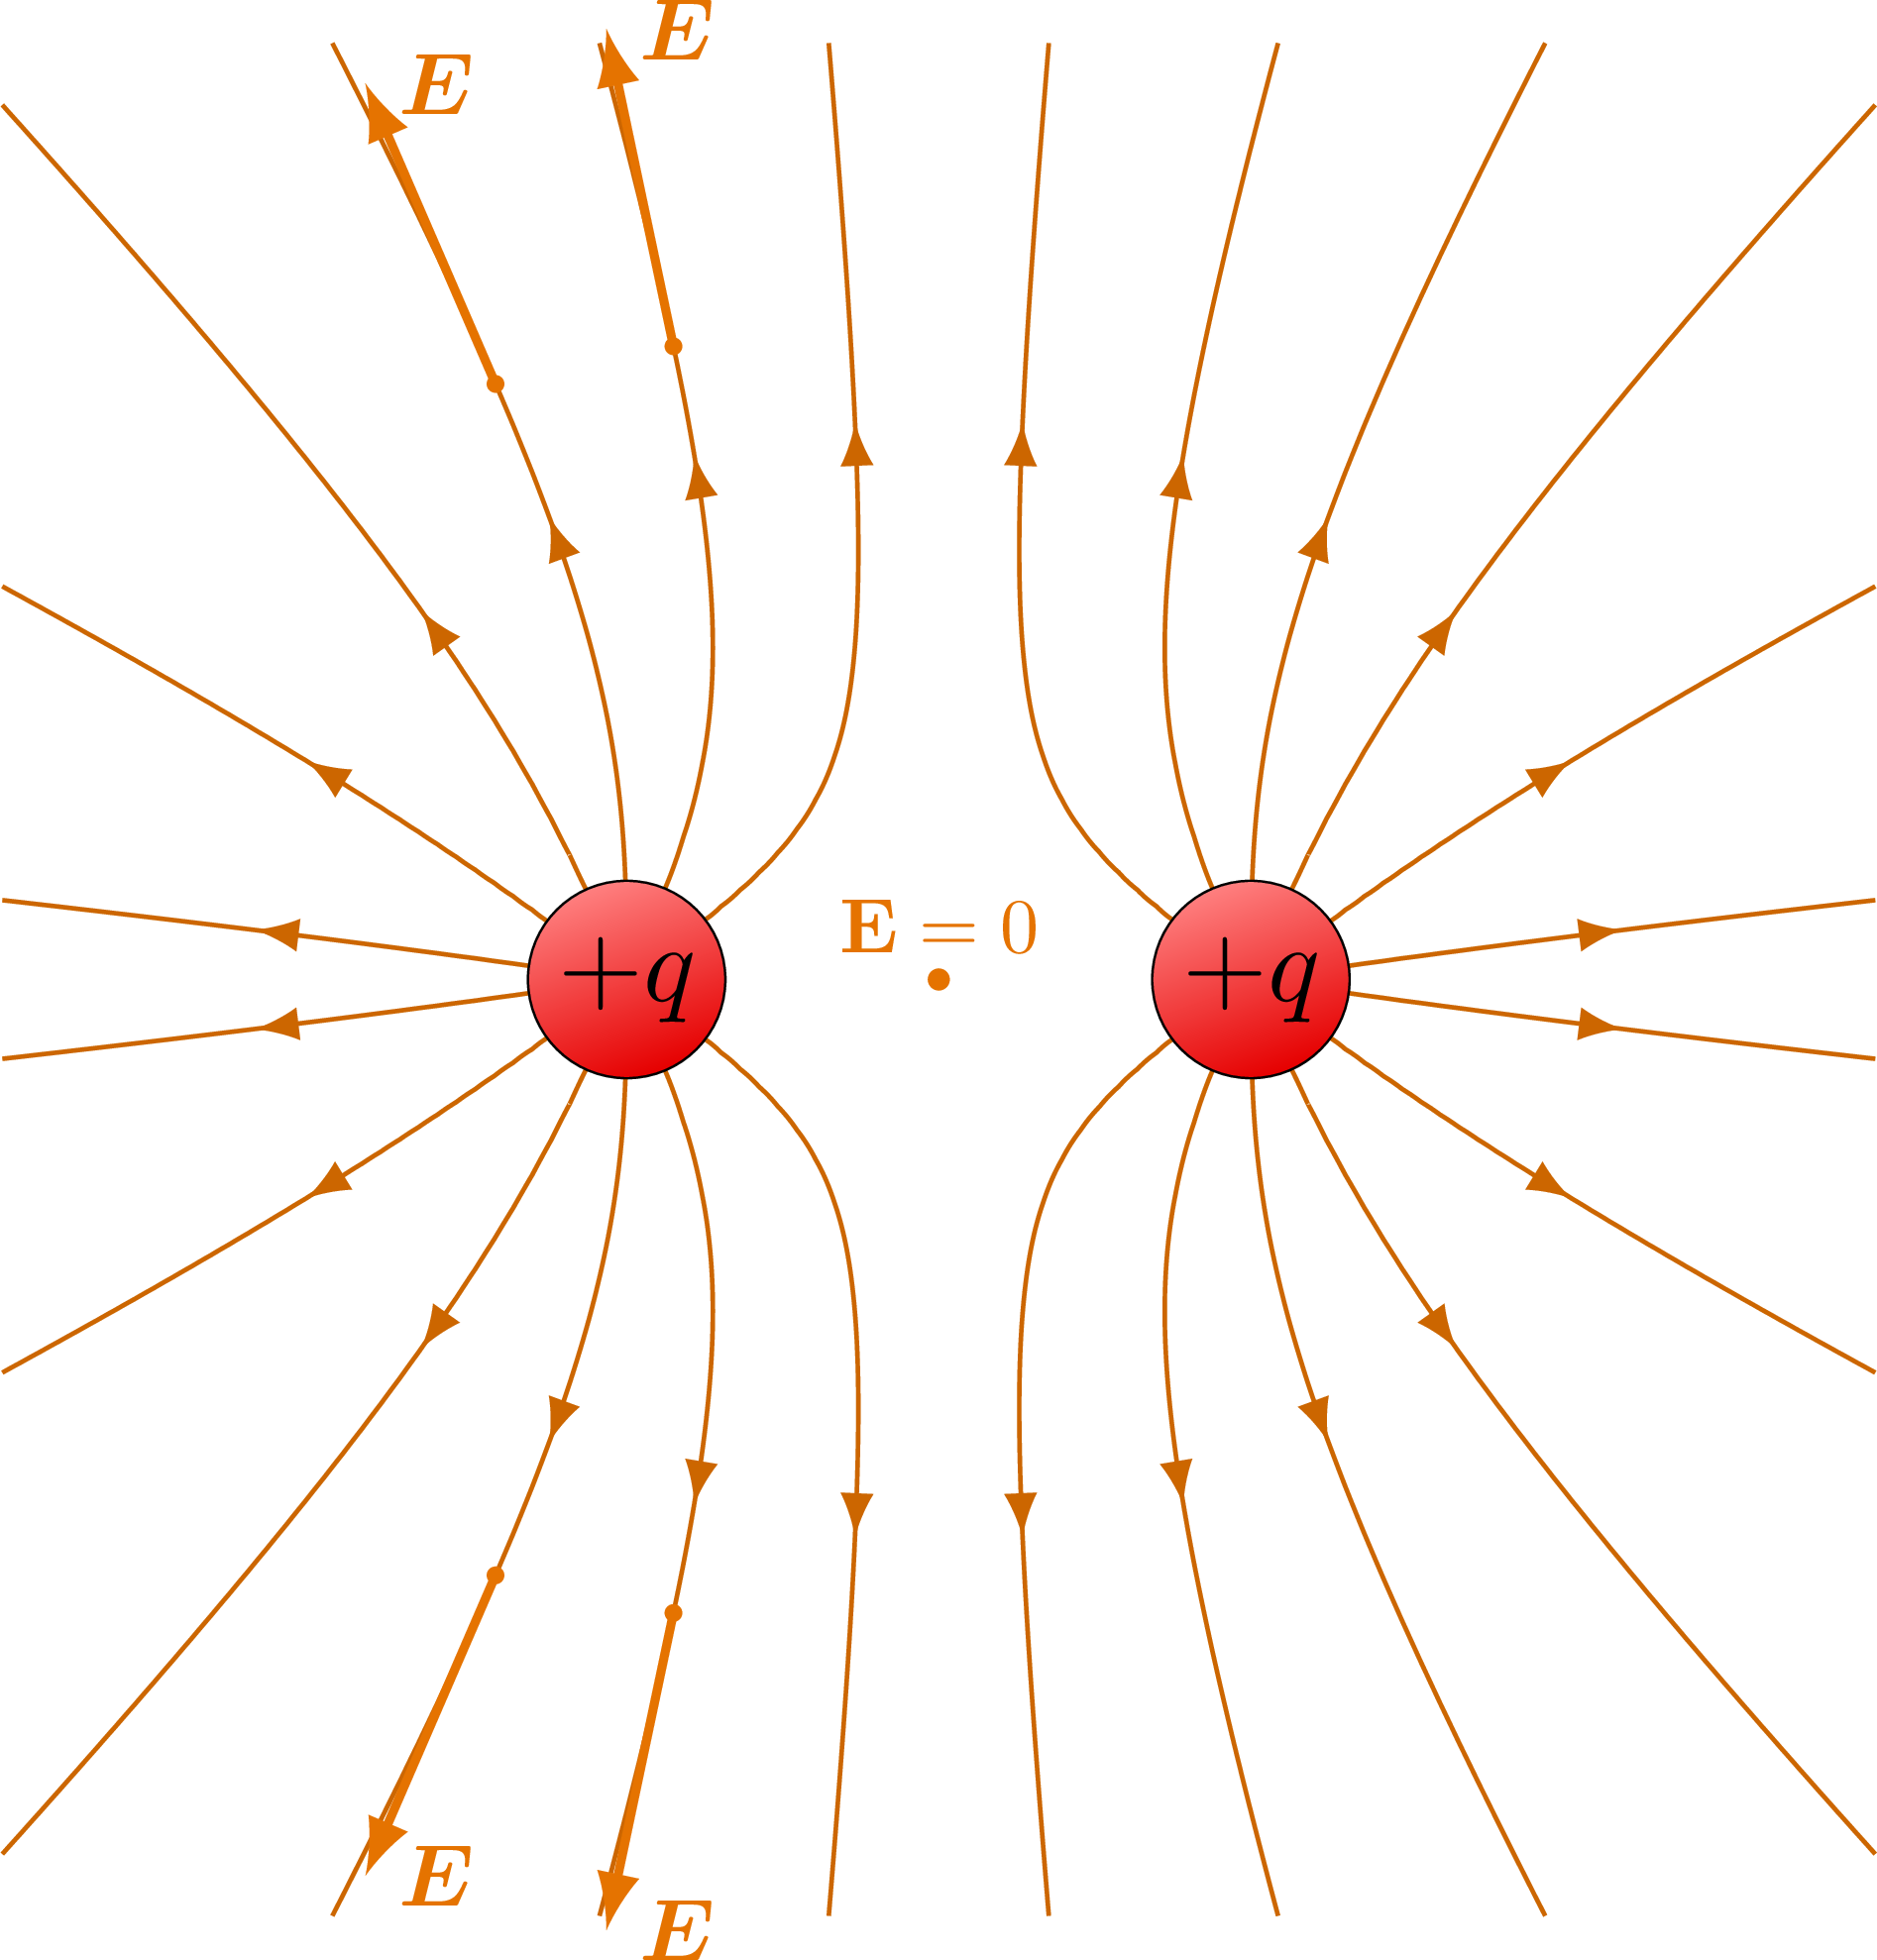
\includegraphics[width = 1\textwidth]{image/interazioniCampiElettrici2.png}
     \end{minipage}
     \caption{Campo elettrico attrattivo a sinistra e repulsivo a destra}
     \label{fig:campoElettricoAttrRep}
 \end{figure}
 
 Per fornire una definizione di campo elettrico consideriamo una carica $Q$. La sola presenza di questa carica modifica attorno ad essa lo spazio circostante, Figura \ref{fig:campoElettricoPosNeg}, e qualsiasi altra carica $Q^*$ che venga introdotta nella regione di spazio in cui agisce il campo generato da $Q$ risentirà di una forza di Coulomb, attraente o repulsiva.
 
 Da qui possiamo allora definire la formula del campo elettrico come:
 
 \begin{equation}
     \vec{E } = \frac{1}{4\pi \varepsilon_0}\frac{Q}{r^2}\vec{u}_r = K_e\frac{Q}{r^2}\vec{u}_r = \frac{\vec{F}}{Q}\qquad\biggl[\frac{N}{C}\biggl]
 \end{equation}
 
 
 \section{Sovrapposizione di campi elettrici}
 Il campo elettrico totale generato da un insieme di cariche in un punto è la
somma vettoriale dei campi elettrici generati da ogni singola carica in quel
punto, dove ciascun campo elettrico va calcolato indipendentemente dagli altri.

La formula per calcolare il campo elettrico totale è la seguente:

\begin{equation}
    \vec{E}_{tot} = \sum_i=1^n \vec{E}_i
\end{equation}

calcolando il modulo del campo elettrico totale avremo:
\begin{equation}
    E_{tot} = K_e\sum_i=1^n \frac{q_i}{r^2}
\end{equation}

\section{Teorema di Gauss per il campo elettrico}
In ogni punto dello spazio attorno a una carica è definito un vettore campo elettrico. L’insieme di questi vettori forma un campo vettoriale che contiene l’informazione relativa alla carica che l’ha creato.

Introduciamo ora una grandezza costituita a partire dal campo elettrico: il \textbf{flusso} attraverso una superficie.

\subsection{Il flusso del campo elettrico}
Il flusso del campo elettrico attraverso una superficie è dato dall'integrale del campo elettrico sulla superficie \footnote{o vettore area} considerata; nel caso di un campo elettrico uniforme e di una superficie piana il calcolo si riduce al prodotto scalare tra il vettore campo elettrico e il vettore superficie.

Per scrivere la definizione di flusso abbiamo bisogno di una superficie limitata nello spazio e un vettore area, il quale ha come modulo l'area e come direzione la retta normale alla superficie nel punto.

\paragraph{}

Il flusso del campo elettrico $\Phi(\vec{E})$ attraverso una superficie qualsiasi esprime, in un certo modo, una misura delle linee di campo elettrico che attraversano la superficie considerata, indipendentemente che sia aperta o chiusa, piana o ricurva.
Supponiamo che $\vec{E}$ sia un campo elettrico uniforme: il suo modulo è costante per ogni punto.

\paragraph{}
Definiamo il flusso del campo elettrico $\vec{E}$ come il prodotto scalare del vettore $\vec{E}$ per il vettore area $\vec{S}$:

\begin{equation}
    \Phi(\vec{E}) = \vec{E}\cdot\vec{S}\qquad\biggl[\frac{N\,m^2}{C}\biggl]
\end{equation}
possiamo scrivere il flusso, essendo un prodotto scalare,  come:
\begin{equation}
    \Phi(\vec{E}) = ES\cos{\theta}
\end{equation}
dove $S$ rappresenta l'area della superficie.
Si può capire che il flusso ha valore massimo quando i vettori campo elettrico sono perpendicolari alla superficie e paralleli al vettore superficie. Mentre assumerà il valore nullo quando la superficie è parallela al campo elettrico.


\def\L{2.2}
\def\H{2.2}
\def\offset{2.0}
\def\W{0.30}
\def\Nx{5}
\def\Ny{5}
\begin{figure}[tb]
    \centering
    
       \begin{tikzpicture}[x={(1.0cm,0)},y={(0.55cm,0.5cm)},z={(0,1.0cm)}]
      \def\H{2.5}
      \def\W{4.8}
      \def\Ny{5}
      \def\Nz{4}
      \def\NEy{4}
      \def\NEz{3}
      \def\oEy{0.08*\W}
      \def\oEz{0.04*\H}
      \def\E{2}
      \coordinate (O) at (0.0,-0.5,-0.5);
      
      % AXES
      \draw[->,thick] (0.5,0,0) --++ (0.5*\H,0,0) node[right] {$x$};
      %\draw[->,thick] (O) --++ (0.5*\H,0,0) node[right] {$x$};
      %\draw[->,thick] (O) --++ (0,0.7*\H,0) node[right] {$y$};
      %\draw[->,thick] (O) --++ (0,0,0.5*\H) node[above] {$z$};
      
      % ELECTRIC FIELD back
      \foreach \i [evaluate={\y=\oEy+(\i-0.5)*(\W-2*\oEy)/\NEy;}] in {1,...,\NEy}{
        \foreach \j [evaluate={\z=\oEz+(\j-0.5)*(\H-2*\oEz)/\NEz;}] in {1,...,\NEz}{
          \draw[EFieldLine,very thick] (0,\y,\z) --++ (-\E,0,0);
        }
      }
      
      % PLANE
      \draw[charged]
        (0,0,0) --++ (0,\W,0) --++ (0,0,\H) --++ (0,-\W,0) -- cycle;
      \foreach \i [evaluate={\y=(\i-0.5)*\W/\Ny;}] in {1,...,\Ny}{
        \foreach \j [evaluate={\z=(\j-0.5)*\H/\Nz;}] in {1,...,\Nz}{
          \node[scale=0.8,rotate=0] at (0,\y,\z) {$+$};
        }
      }
      
      % ELECTRIC FIELD front
      \foreach \i [evaluate={\y=\oEy+(\i-0.5)*(\W-2*\oEy)/\NEy;}] in {1,...,\NEy}{
        \foreach \j [evaluate={\z=\oEz+(\j-0.5)*(\H-2*\oEz)/\NEz;}] in {1,...,\NEz}{
          \draw[EFieldLine,very thick] (0,\y,\z) --++ (\E,0,0);
        }
      }
      \node[Ecol] at (1.3,0.88*\W,0.88*\H) {$\vb{E}$};
     
    \end{tikzpicture}
    \caption{Flusso massimo, il piano è ortogonale al campo elettrico }
    \label{fig:flussoMassimo}

\end{figure}

\section{La legge di Gauss}
\label{teoremaGauss}

Il teorema di Gauss afferma che il flusso di un campo elettrico di una superficie chiusa è dato dal rapporto tra carica elettrica totale interna alla superficie e la costante dielettrica.

\begin{equation}
    \Phi(\vec{E})  =\frac{Q}{\varepsilon_0}
\end{equation}

\subsection{Dimostrazione del teorema di Gauss}
Per dimostrarlo consideriamo una superficie sferica, con una carica puntiforme collocata al centro della sfera.

\def\L{2.2}
\def\H{2.2}
\def\W{0.30}
\def\Nx{5}
\def\Ny{5}
\begin{figure}
    \centering
    \begin{tikzpicture}
      \def\N{7}
      \def\R{2.2}
      \def\r{0.8}
      
      % SPHERE BACK
      \begin{scope}
        \clip (-\R,0) rectangle ++(2*\R,\R);
        \draw[gauss line,very thin,dashed]
          (0,0) ellipse ({\R} and {\r});
      \end{scope}
      
      % CHARGES
      \node[charge+,scale=0.8,circle,inner sep=0.27] (C) at (0,0) {$+Q$};
      
      % FIELD LINES
      \path[name path=ell](0,0) ellipse ({0.78*\R} and {\R});
      \foreach \i [evaluate={\ang=-8+\i*360/\N;}] in {1,...,\N}{
        %\message{Eline\i^^J}
        \draw[EFieldLine,name path global/.expanded=Eline\i] (C) -- ({1.2*\R*cos(\ang)},{1.3*\R*sin(\ang)}) coordinate (E\i);
        %(\ang:1.3*\R)
      }
      
      % SPHERE
      \draw[gauss line,ball color=green!70!black,fill opacity=0.1]
        (0,0) circle (\R);
      \begin{scope}
        \clip (-\R,0) rectangle ++(2*\R,-\R);
        \draw[gauss line,very thin]
          (0,0) ellipse ({\R} and {0.3*\R});
      \end{scope}
      \draw[<->,gauss line,very thin]
        (C) -- (190:{\R} and {\r}) node[measure] {$R$}; %{\contour{green!70!black!7}{$R$}};
      
      % VECTOR
      \draw[gauss dark,name intersections={of={Eline1} and ell,name=ES1}]
        (ES1-1) ++ (-0.081*\R,0.033*\R) to[out=20,in=180] ++(10:0.09*\R)
                                        to[out=-35,in=115] ++(-50:0.09*\R)
                                        to[out=185,in=15] ++(190:0.09*\R)
                                        to[out=120,in=-40] cycle; %node[left] {$\dd{A}$};
      \node[green!40!black,right=5,below=2] at (ES1-1) {$\dd{S}$};
      \foreach \i [evaluate={\angle=8+\i*360/\Nx;}] in {1,6,7}{
        \draw[EField,-,name intersections={of={Eline\i} and ell,name=ES\i}] (ES\i-1) -- (E\i);
      }
      \draw[normalvec] (ES1-1) ++ (138:0.03*\R) --++ (50:0.16*\R) node[above=-1] {$\vec{s}$};
      
    \end{tikzpicture}
    \caption{Carica puntiforme nel centro della sfera}
    \label{fig:caricaPuntiformeGauss}
\end{figure}


Siccome la carica interna è positiva, le linee di campo sono uscenti, dunque tale è anche il verso di $\vec{E}$.

Se cercassimo ora di dividere la superficie sferica in tantissime parti, otterremo tante superfici infinitesime $dS$ che inevitabilmente risulteranno una superficie piana in cui il campo su ciascuna superficie infinitesima possa essere considerato uniforme. Questo ragionamento è applicabile a qualsiasi superficie chiusa $S$, detta superficie gaussiana, immersa in un campo elettrico.

Il flusso totale del campo elettrico sarà dato dalla somma di tutti i contributi delle superfici infinitesime $dS$ della sfera.
Visto che stiamo considerando una superficie infinitesima, anche il relativo contributo del flusso deve essere infinitesimo e dunque scriveremo:

\begin{equation*}
    d\Phi = \vec{E}\cdot d\vec{S}
\end{equation*}

tale prodotto scalare diventa:

\begin{equation*}
    d\Phi = Eds\cos{0} = EdS
\end{equation*}

per ottenere la somma di tutti i flussi infinitesimi dobbiamo integrare su tutta la superficie, dunque:

\begin{equation*}
    \Phi(\vec{E}) = \oint_s \vec{E}\cdot d\vec{S} = \int_s d\Phi = \int_s Eds
\end{equation*}
Essendo una superficie piana il campo elettrico è costante e si può portare fuori dall'integrale:
\begin{equation*}
    \Phi(\vec{E})  = E\int_s ds  = ES
\end{equation*}

nel nostro caso la superficie $S$ si tratta di una superficie sferica e, a questo punto,  sostituendo ci siamo ricondotti al teorema di Gauss:

\begin{equation}
    \Phi(\vec{E}) = \frac{1}{4\pi\varepsilon_0}\frac{Q}{r^2}4\pi r^2 = \frac{Q}{\varepsilon_0}
\end{equation}

\paragraph{}
Risolvendo l'equazione del teorema di Gauss otteniamo:
\begin{equation*}
     \Phi(\vec{E}) = \frac{Q}{\varepsilon_0}
\end{equation*}

\begin{equation*}
     \oint_s \vec{E}\cdot d\vec{S} = \frac{Q}{\varepsilon_0}
\end{equation*}

\begin{equation*}
     E\int_s dS = \frac{Q}{\varepsilon_0}
\end{equation*}

la superficie di una sfera è $4\pi r^2$ e dunque:
\begin{equation*}
    \Phi(E) = E4\pi r^2
\end{equation*}
\begin{equation*}
     E4\pi r^2 = \frac{Q}{\varepsilon_0}
\end{equation*}

\begin{equation*}
     E = \frac{Q}{4\pi\varepsilon_0r^2}
\end{equation*}

possiamo capire ora che la legge di Coulomb è una conseguenza del teorema di Gauss.



\section{Campo elettrico cavo infinito}
\label{paginaCampoElettricoCavoInfinito}


\def\L{8}
\def\W{0.25}
\def\N{14}
\def\M{4}
 \def\ymax{\L/3}
\begin{figure}[H]
    \centering
    \begin{tikzpicture}[rotate = -90, scale = 0.8]
      \def\R{0.4*\L}
      \def\g{0.2*\R}
      \def\G{0.6*\R}
      \def\a{0.33*\L}
      \coordinate (L)  at (-\a,0);
      \coordinate (R)  at (+\a,0);
      \coordinate (TL) at (-\a,\G);
      \coordinate (TR) at (+\a,\G);
      \coordinate (BL) at (-\a,-\G);
      \coordinate (BR) at (+\a,-\G);
      
      % GAUSS BEHIND
      \draw[gauss line,dashed] (TR) arc (90:270:{\g} and {\G});
      
      % ROD
      \draw[charged] (-\L/2,-\W/2) --++(\L,0) to[out=0,in=0] ++ (0,\W) --++ (-\L,0) -- cycle;
      \draw[charged] (-\L/2,-\W/2) to[out=180,in=180] ++ (0,\W) to[out=0,in=0] cycle;
      \foreach \i [evaluate={\x=-\L/2+\i*\L/(\N+1);}] in {1,...,\N}{
        \node[scale=0.6] at (\x,0) {$+$};
      }
      \begin{scope}
        \clip (-\L/2,-0.5*\W)
          --++ (\L/2-\a,0) to[out=50,in=-50] ++(0,1.0*\W) --++ (-\L/2+\a,0) --++ (0,\G)
          --++ (\L-2*\a,0) --++ (0,{-2*(\G+\W)}) --++ (-\L+2*\a,0) -- cycle;
        \draw[gauss lid] (L) ellipse ({\g} and {\G});
      \end{scope}
      
      
      % GAUSS IN FRONT
      \draw[<->] (-\a,-\W/2) -- (-\a,-\G) node[measure,fill=green!80!black!8,inner sep=1,outer sep=0] {$r$};
      \draw[<->] (-\a,-1.1*\G) -- (\a,-1.1*\G) node[measure] {$L$};
      \draw[gauss surf]
        (BL) arc (-90:90:{\g} and {\G}) --
        (TR) arc (90:-90:{\g} and {\G}) -- cycle;
      \draw[normalvec] (-0.064*\L,\G) --++ (0,0.25*\G) node[left=2,above] {$\vu{n}$};
      \draw[->,thick,Ecol] (-0.045*\L,\G) --++ (0,0.6*\G) node[right] {$\vb{E}$};
      
      \draw[->,thick,Ecol] (-\a,1) --++ (0,2.08) node[right] {$\vb{E}$};
      
      % LABELS
      \node[left,green!30!black] at ($(-\a,0)+(150:{\g} and {\G})$) {$S_1$};
      \node[right,green!30!black] at ($(\a,0)+(30:{\g} and {\G})$) {$S_2$};
      \node[above,green!30!black] at (0.6*\a,\G) {$S_3$};
      
  
    \end{tikzpicture}
    \caption{Campo elettrico attorno ad un filo infinito}
    \label{fig:campoElettFiloInf}
\end{figure}



Con questo esempio vogliamo studiare quale sia il flusso che attraversa il cilindro.
Sappiamo che il flusso totale ha la seguente formula:

\begin{equation*}
    \Phi_t(E) = E\int_{sup. lat.}dS
\end{equation*}
la superficie esterna del cilindro la sappiamo calcolare e dunque il flusso sarà:
\begin{equation*}
    \Phi(E) = E2\pi rh
\end{equation*}
\begin{equation*}
    E2\pi rh = \frac{\lambda h}{\varepsilon_0}
\end{equation*}
\begin{equation}
    E = \frac{\lambda}{2\pi r\varepsilon_0}  = \frac{\rho_{0}\pi r^2}{2\pi r\varepsilon_0}
    \label{leggeDiGaussDim}
\end{equation}

Dove $\lambda\,[\frac{C}{m}]$ indica la densità di carica nel filo.
\paragraph{}
Sulle basi $S_1$ e $S_2$ il campo elettrico è parallelo alla base e il prodotto \\$\vec{E}\cdot d\vec{s} = Edscos\theta$ è nullo in quanto il coseno è zero.
 
\section{Piano infinito}
\label{pianoInfinito}

\begin{figure}[H]
    \centering
    \begin{tikzpicture}[x={(1.0cm,0)},y={(0.55cm,0.5cm)},z={(0,1.0cm)}, scale = 1.3]
      \def\H{2.5}
      \def\W{4.8}
      \def\Ny{5}
      \def\Nz{4}
      \def\R{0.14*\W}
      \def\a{0.49*\H}
      \def\E{0.36*\H}
      \def\plane{(0,0,0) --++ (0,\W,0) --++ (0,0,\H) --++ (0,-\W,0) -- cycle;}
      \coordinate (O) at (0.0,-0.5,-0.5);
      \coordinate (C)  at (      0,\W/2,\H/2);
      \coordinate (ER) at (     \a,\W/2,\H/2);
      \coordinate (EL) at (-1.2*\a,\W/2-0.6*\R,\H/2+0.5*\R);
      \coordinate (TM) at (      0,\W/2,\H/2+\R);
      \coordinate (TR) at (     \a,\W/2,\H/2+\R);
      \coordinate (TL) at (-1.2*\a,\W/2,\H/2+\R);
      \coordinate (BM) at (      0,\W/2,\H/2-\R);
      \coordinate (BR) at (     \a,\W/2,\H/2-\R);
      \coordinate (BL) at (-1.2*\a,\W/2,\H/2-\R);
      \coordinate (NT) at (0.7*\a,\W/2,\H/2+\R);
      \coordinate (NR) at (\a,\W/2+0.13*\R,\H/2+0.13*\R);
      \coordinate (NL) at (-1.2*\a,\W/2-0.5*\R,\H/2-0.2*\R);
      \coordinate (NB) at (0.86*\a,\W/2-0.6*\R,\H/2-0.6*\R);
      
      % AXES
      \draw[->,thick] (0.5,0,0) --++ (0.5*\H,0,0) node[right] {$x$};
      
      % VECTORS back
      \draw[EField] (EL) --++ (-\E,0,0);
      \draw[normalvec] (EL) ++(0,-0.1*\R,-0.13*\R) --++ (-0.5,0,0) node[below left=-4] {$\vu{n}$};
      \draw[gauss dark]
        (EL)++(0,-0.1*\R,-0.3*\R)
          to[out=0,in=0,looseness=1.2] ++(0,0,0.5*\R)
          to[out=180,in=180,looseness=1.2] ++(0,0,-0.5*\R) -- cycle; %node[left=4,below=-1] {$\dd{A}$};
      
      % GAUSSIAN SURFACE back
      \draw[gauss dashed line] (BL) to[out=0,in=0,looseness=1.2] (TL);
      \draw[gauss surf]
        (BM) to[out=180,in=180,looseness=1.2] (TM) --
        (TL) to[out=180,in=180,looseness=1.2] (BL) -- cycle;
      
      % PLANE
      \draw[charged] \plane;
      \begin{scope}
        \clip \plane;
        \draw[gauss dashed line] (BM) -- (BL);
        \draw[gauss dashed line] (TM) -- (TL);
        \draw[gauss dashed line] (BL) to[out=0,in=0,looseness=1.2] (TL);
      \end{scope}
      \foreach \i [evaluate={\y=(\i-0.5)*\W/\Ny;}] in {1,...,\Ny}{
        \foreach \j [evaluate={\z=(\j-0.5)*\H/\Nz;}] in {1,...,\Nz}{
          \node[scale=0.8,rotate=0] at (0,\y,\z) {$+$};
        }
      }
      \draw[gauss dark]
        (NT) ++ (-0.12,0,0) to[out=-5,in=110] ++(0,0.12,-0.10) --++(0.22,0,0) to[out=110,in=-5] ++(0,-0.12,0.10) -- cycle;
      
      % GAUSSIAN SURFACE front
      \draw[gauss dashed line]
        (BM) to[out=0,in=0,looseness=1.2] (TM);
      \draw[gauss surf]
        (BM) to[out=180,in=180,looseness=1.2] (TM) --
        (TR) to[out=180,in=180,looseness=1.2] (BR) -- cycle;
      \draw[gauss lid]
        (BR) to[out=0,in=0,looseness=1.2] (TR) to[out=180,in=180,looseness=1.2] cycle;
      
      % DARK
      \draw[gauss dark]
        (NT) ++ (-0.12,0,0) to[out=-160,in=80] ++(0,-0.12,-0.05) --++(0.22,0,0) to[out=80,in=-160] ++(0,0.12,0.05) -- cycle;
      \draw[gauss dark]
        (ER)++(0,0.1*\R,-0.2*\R)
          to[out=0,in=0,looseness=1.2] ++(0,0,0.5*\R)
          to[out=180,in=180,looseness=1.2] ++(0,0,-0.5*\R) -- cycle node[left = -3, below=-3] {$\dd{A}$};
      
      % ELECTRIC FIELD
      \draw[EField] (ER) --++ (\E,0,0) node[right] {$\vb{E}$};
      \draw[EField] (NT) --++ (\E,0,0) node[right] {$\vb{E}$};
      
      % VECTORS
      \draw[normalvec] (ER) ++(0,0.1*\R,0.13*\R) --++ (0.5,0,0) node[above=3,right=-2] {$\vu{n}$};
      \draw[normalvec] (NT) --++ (0,0,0.5) node[below=1,left=-1] {$\vu{n}$};
      %\draw[normalvec] (NB) --++ (0,-0.35,-0.25) node[below right=-2] {$\vu{n}$};
      
      
    \end{tikzpicture}
    \caption{Piano infinito}
    \label{fig:pianoInfnito}
\end{figure}
 
Con questo esempio vogliamo studiare quale sia il flusso che attraversa il cilindro.
Sappiamo che il flusso totale ha la seguente formula:

\begin{equation*}
    \Phi_t(E) = E\int_{base 1}dS + E\int_{base 2}dS
\end{equation*}
la superficie esterna del cilindro la sappiamo calcolare e dunque il flusso sarà:
\begin{equation*}
    \Phi(E) = E2\pi r^2
\end{equation*}
\begin{equation*}
    E2\pi r^2 = \frac{\sigma}{\varepsilon_0}
\end{equation*}
\begin{equation}
    E = \frac{\sigma}{2\varepsilon_0}
\end{equation}

Dove $\sigma \frac{C}{m^2}$ indica la densità di carica nel piano.

\section{Calcolare il campo elettrico ad una distanza arbitraria da un filo}

\begin{figure}[H]
    \centering
    \begin{tikzpicture}[scale = 1, rotate = -90]
          \def\xmax{0.6*\L}
          \def\ymin{-0.18*\L}
          \def\ymax{0.5*\L}
          \def\x{0.342*\L}
          \def\dx{0.05*\L}
          \coordinate (O) at (0,0);
          \coordinate (P) at (0,{0.6*\ymax});
          \coordinate (X) at (\x,\W/2);
          
          % AXIS
          \draw[->,thick] (\xmax, 0) -- (-\xmax,0) node[left] {$y$};
          \draw[->,thick] (0,\ymin) -- (0,\ymax) node[below] {$x$};
          
          % MEASURES
          %\draw[<->] (0,0.2*\ymax) --++ (\x,0) node[midway,above] {$x$};
          \draw[<->] (    0,0.25*\ymin) --++ (\x,0) node[measure] {$y$};
          \draw[<->] (   \x,0.25*\ymin) --++ (\dx,0) node[midway,left] {$dy$};
          \draw[<->] (-\L/2,0.62*\ymin) --++ (\L,0) node[measure, below = 10] {$L$};
          
          % VECTORS
          \draw[EField,very thick] (P) --++ ( 0.0,0.6) node[right=7, below] {$\dd{\vb{E}_x} = \vec{j}\cos\theta$};
          \draw[EField,very thick] (P) --++ (-0.6,0.0) node[left=-1] {$\dd{\vb{E}_y} = \vec{j}\sin\theta$};
          \draw[EField,very thick] (P) --++ (-0.6,0.6) node[above left=-2] {$\dd{\vb{E}}$};
          \draw[EField,-,dashed,thin] (P) ++ (0,0.6) --++ (-0.6,0) --++ (0,-0.6);
          
          % POINT
          \fill (P) circle (0.06) node[below=8,right=1] {P};
          \draw[<->] (-0.25,0.2) --++ (0,2.1) node[measure] {$r$};
          \draw[dashed] (P) -- (X) node[measure]{$R$};
          \draw pic[->,"$\theta$",draw=black,angle radius=20,angle eccentricity=1.4] {angle = O--P--X};
          \draw[vector] (X) -- ($(X)!0.12!(P)$) node[above] {$\vu{r}$};
          
          % ROD
          \draw[charged] (-\L/2,-\W/2) rectangle ++(\L,\W);
          \draw[darkcharged] (\x,-\W/2) rectangle ++(\dx,\W)
            node[above, right] {$\dd{q}=\lambda \dd{x}$};
          \foreach \i [evaluate={\x=-\L/2+\i*\L/(\N+1);}] in {1,...,\N}{
            \node[scale=0.6] at (\x,0) {$+$};
          }

    \end{tikzpicture}
    \caption{Campo elettrico ad una distanza $R$ da un filo}
    \label{fig:campoElettDistanzaRFilo}
\end{figure}

Prendendo un pezzo di filo rettilineo, vogliamo studiare cosa succede in un suo pezzo; il filo può essere anche asimmetrico.

Utilizzando la legge di Coulomb, che non dipende dalle simmetrie, possiamo ricavarci il campo elettrico infinitesimo generato in ogni punto e sommare, con un integrale, tutti i punti del filo:

\begin{equation*}
    d\vec{E}  = \frac{1}{4\pi \varepsilon_0}\frac{dq}{R^2}\hat{r}
\end{equation*}
indichiamo con $dq$ la carica infinitesima del filo data dal rapporto infinitesimo $\lambda = \frac{dq}{dy}$ e $\hat{r}$ il versore diretto dalla carica  verso il punto $P$.

Prendendo un pezzo infinitesimo di filo, $dx$

Sapendo che il campo infinitesimo è dato da:
\begin{equation*}
    d\vec{E} = d\vec{E_x}\vec{i} + d\vec{E_j}\vec{j}
\end{equation*}

Per calcolare il campo elettrico in $P$ dobbiamo servirci degli integrali e dunque:
\begin{equation*}
   \int d\vec{E} = \int d\vec{E_x}\vec{i} + \int d\vec{E_j}\vec{j}
\end{equation*}
\begin{equation*}
   \int_L \frac{1}{4\pi \varepsilon_0}\frac{dq}{R^2}\hat{r}
\end{equation*}

Notiamo che $dy$, $R^2$ e $\hat{r}$ dipendono dalla posizione $y$. Dobbiamo cercare di scrivere tutto in funzione di una singola variabile.

La variabile che più si addice a tale scopo è: $\theta$, l'angolo che viene formato dal punto $dy$ al punto in cui vogliamo calcolare il campo, $P$.

\begin{equation*}
    \frac{y}{r} = \tan\theta\quad\rightarrow\quad y = r\tan\theta
\end{equation*}

\begin{equation*}
     dy = \frac{dy}{d\theta}d\theta
\end{equation*}
deriviamo $y$ trovata prima rispetto a $\theta$ per trovare la nuova variabile di integrazione:
\begin{equation*}
     dy = r\frac{d\theta}{\cos^2\theta}d\theta
\end{equation*}

infine:

\begin{equation*}
    r = r\cos\theta\quad\rightarrow\quad R = \frac{r}{\cos\theta}
\end{equation*}

ora tutte le parti variabili sono funzioni della stessa parte variabile: l'angolo.

Ora possiamo sommare 
\begin{equation*}
    \int_{\theta_1}^{\theta_2} \frac{1}{4\pi \varepsilon_0}\frac{\lambda r d\theta}{\cos^2\theta}\frac{\cos^2\theta}{r^2}[\cos\theta\vec{i} - \sin\theta\vec{j}]
\end{equation*}

\begin{equation*}
    \frac{\lambda}{4\pi \varepsilon_0 r} \biggl[\biggl( \int_{\theta_1}^{\theta_2} \cos\theta d\theta \biggl)\vec{i} + \biggl(\int_{\theta_1}^{\theta_2} -\sin\theta d\theta \biggl)\vec{j}\biggl]
\end{equation*}

\paragraph{}
Risolvendo troviamo che il campo elettrico nel punto $P$ è:
\begin{equation}
    \vec{E}_{(p)}  = \frac{\lambda}{4\pi \varepsilon_0 r}[(\sin\theta_2 - \sin\theta_1)\,\vec{i}\,  + (\cos\theta_2 - \cos\theta_1)\,\vec{j}\,]
\end{equation}

\paragraph{}
Alcune considerazioni finali...\\
se il filo lo metto in modo tale da avere una simmetria rispetto l'asse $y$ allora l'equazione diventa:

\begin{equation}
    \vec{E}_{(p)}  = \frac{\lambda}{4\pi \varepsilon_0 r}[(\sin\theta_2 - \sin\theta_1)\,\vec{i}\,]
\end{equation}

\paragraph{Se il filo fosse infinito?}
Se il filo fosse infinito avremo che $\theta = \frac{\pi}{2}$

\begin{equation*}
    \vec{E}_{(p)} = \frac{\lambda}{4\pi \varepsilon_0 r}[1-(-1)\,\vec{i}\,] = \frac{\lambda}{2\pi \varepsilon_0 r}\vec{i}
\end{equation*}

e questo segue la dimostrazione del teorema di Gauss, Pagina \pageref{paginaCampoElettricoCavoInfinito}.

\section{Disco}


\begin{figure}[H]
    \centering
    \begin{tikzpicture}[x={(1,0)},y={(0,0.5)}, scale = 1.3]
      \def\R{2.6}
      \def\r{1.35}
      \def\dr{0.52}
      \def\Ex{0.6}
      \def\Ey{1.1}
      \def\Nx{4}
      \coordinate (O) at (0,0);
      \coordinate (P) at (0,4.0);
      \coordinate (Y) at (0,6.0);
      \coordinate (R) at (\r,0);
      
      % PLANE
      \draw[charged]
        (O) circle (\R);
      \draw[darkcharged,even odd rule]
        (O) circle (\r+\dr) circle (\r);
      \foreach \i [evaluate={\cr=(\i-0.5)*\R/\Nx; \Ny=7+4*(\i-2);}] in {1,...,\Nx}{
        \foreach \j [evaluate={\cang=39+\j*360/\Ny;}] in {1,...,\Ny}{
          \node[scale=0.8,rotate=0] at (\cang:\cr) {$+$};
        }
      }
      
      % CHARGE
      \node[right=-1.5,scale=0.9] at (4:\r+\dr) {$\dd{q}=\sigma \dd{S}$};
      
      % AXIS
      \draw[->,thick] (0,0) -- (Y) node[above] {$z$};
      
      % VECTORS
      \draw[EField,very thick] (P) --++ ( 0.0,\Ey) node[right=1] {$\dd{\vb{E}_y}$};
      \draw[EField,very thick] (P) --++ (-\Ex,0.0) node[left=2] {$\dd{\vb{E}_x}$};
      \draw[EField,very thick] (P) --++ (-\Ex,\Ey) node[above left=-2] {$\dd{\vb{E}}$};
      \draw[EField,-,dashed,thin] (P) ++ (0,\Ey) --++ (-\Ex,0) --++ (0,-\Ey);
      \node[fill=blue!60!black,circle,inner sep=1.1] (P') at (P) { };
      \node[above=3,right=1] at (P') {P};
      \draw[vector,veccol] (R) -- (P') node[pos=0.8,right=3] {$\vb{L}$};
      \draw[vector,veccol] (0,0) --++ (0:\r) node[pos=0.7,above=-1] {$\vb{r}$};
      \draw[<->] (0,0) --++ (-101:\R) node[pos=0.35,right=-2] {$R$};
      
      \draw[->,thick] (-3,-3) --++ (6,6) node[right = 3] {$y$};
      \draw[->,thick] (-3,3) --++ (6,-6) node[right = 3] {$x$};
      
      
    \end{tikzpicture}
    \caption{Disco infinito}
    \label{fig:discoInfinito}
\end{figure}

ogni superficie infinitesima è:
\begin{equation*}
    dq = \sigma ds = \sigma rd\theta dr
\end{equation*}

\begin{equation*}
    d\vec{E_z} = \int_{disco} \frac{1}{4\pi \varepsilon_0}\frac{dq}{r'}\cos\alpha \vec{k}
\end{equation*}
$\vec{k}$ è il versore dell'asse z

\begin{equation*}
   \frac{\sigma h 2\pi}{4 \pi \varepsilon_0}\int_0 ^R (h^2+r^2)^{-\frac{3}{2}} rdr
\end{equation*}

Ora per sommare tutte le piastrelline, i contributi, devo prima sommarle tutte sulla medesima circonferenza e poi sommare tutte le circonferenze per ottenere il disco.

\begin{equation*}
   \int_{0_{(\theta)}} ^ {2\pi} \int_{0_{(r)}} ^ {R} \frac{1}{4\pi \varepsilon_0}\frac{\sigma dr rd\theta}{(h^2 + r^2)}\frac{h}{(h^2 + r^2)^\frac{1}{2}} \vec{K}
\end{equation*}
\begin{equation*}
   \frac{\sigma h 2\pi}{4 \pi \varepsilon_0}\int_0 ^R (h^2+r^2)^{-\frac{3}{2}} rdr
\end{equation*}
\begin{equation*}
   \frac{\sigma h}{2\varepsilon_0} \frac{1}{2}\int_0 ^R (h^2+r^2)^{-\frac{3}{2}} 2rdr
\end{equation*}
\begin{equation*}
   \frac{\sigma h}{2\varepsilon_0} \frac{1}{2}\int_0 ^R (h^2+r^2)^{-\frac{3}{2}} d(r^2)
\end{equation*}
\begin{equation*}
   \frac{\sigma h}{2\varepsilon_0} \frac{1}{2} \biggl[ \frac{(h^2+r^2)}{-\frac{1}{2}} \biggl]_0 ^R
\end{equation*}

\begin{equation*}
   \frac{\sigma h}{2\varepsilon_0} [ -(h^2+ R^2)^{-{\frac{1}{2}}} + h^{-1}]
\end{equation*}
\begin{equation}
   \vec{E} = \frac{\sigma}{2\varepsilon_0} \bigg[ 1 - \frac{h}{\sqrt{h^2 + R^2}}\bigg]\vec{K}
\end{equation}

\paragraph{Cosa ottengo se il disco fosse infinito?}
Se il disco fosse infinito devo ottenere il medesimo risultato che ottengo con Gauss per un piano infinito.

Se il disco diventa infinito, allora $R$ tende a infinito e dunque:
\begin{equation}
    \vec{E} = \frac{\sigma}{2\varepsilon_0} [ 1 - 0] = \frac{\sigma}{2\varepsilon_0}
\end{equation}

ed infatti è proprio lo stesso risultato che otteniamo con un piano infinito, Pagina \pageref{pianoInfinito}.

\paragraph{Se il raggio del cilindro lo tendiamo a zero, ovvero ad un punto?} 
Dovrebbe restituire proprio la legge di Coulomb.
\begin{equation*}
    \vec{E} = \frac{\sigma}{2\varepsilon_0} [ 1 - 1] = \frac{\sigma}{2\varepsilon_0}
\end{equation*}
\begin{equation}
    \vec{E} = 0
\end{equation}

Ma questo non è vero perché far tendere a zero un disco significa anche mandare a zero la sua carica. Nel nostro caso invece la carica la vogliamo mantenere inalterata.
\paragraph{}
Quindi cerchiamo di scriverla in modo diverso:

\begin{equation*}
   \vec{E} = \frac{\sigma}{2\varepsilon_0} \bigg[ 1 - \frac{h}{\sqrt{h^2 + R^2}}\bigg]\vec{K}
\end{equation*}
\begin{equation*}
    \vec{E} = \frac{\sigma}{2\varepsilon_0} \Biggl[ 1 - \frac{h}{h\sqrt{1 + \frac{R^2}{h^2} }}\Biggl]\vec{K}
\end{equation*}
\begin{equation*}
    \vec{E} = \frac{\sigma}{2\varepsilon_0} \Biggl[ 1 - \frac{1}{\sqrt{1 + \frac{R^2}{h^2} }}\Biggl]\vec{K}
\end{equation*}

Ora per trovare la soluzione corretta dobbiamo utilizzare lo sviluppo di Taylor applicato a: 

\begin{equation*}
    f(x) = \frac{1}{\sqrt{1 - x}} = (1-x)^{-\frac{1}{2}} = f(0) + f'(0)x + f''(0)x^2 + \dots
\end{equation*}
\begin{equation*}
    f'(x) = -\frac{1}{2}(1-x)^{-\frac{3}{2}}
\end{equation*}

arrestandoci al $1 \gradi$ ordine otteniamo che:

\begin{equation*}
    f(x) = \frac{1}{\sqrt{1 - x}} = 1 - \frac{1}{2}x
\end{equation*}

Quindi il campo lo riscriviamo come:

\begin{equation*}
    \vec{E} = \frac{\sigma}{2\varepsilon_0 } \Biggl[ 1 - 1 + \frac{1}{2}x\Biggl]\vec{K}
\end{equation*}
sostituendo $x$
\begin{equation*}
    \vec{E} = \frac{\sigma}{2\varepsilon_0} \Biggl[ 1 - 1 + \frac{1}{2}\frac{R^2}{h^2}\Biggl]\vec{K}
\end{equation*}

\begin{equation*}
    \vec{E} = \frac{\sigma R^2 \pi}{ \pi 2\varepsilon_0 2 h^2}
\end{equation*}
moltiplicando sopra e sotto per $\pi$ otteniamo che a numeratore abbiamo $\sigma$ per la superficie del disco $\pi R^2$ che corrisponde alla carica Q.

\begin{equation*}
    \vec{E} = \frac{Q}{ 4 \pi \varepsilon_0  h^2}
\end{equation*}

E questa è la legge di Coulomb.
L'errore è proporzionale alla variabile stessa, infatti continuando la serie di Taylor otteniamo che i termini di grado superiore al primo vanno a zero più rapidamente.


\section{Campo elettrico di una sfera dielettrica}

\begin{figure}[H]
    \centering
    \begin{minipage}[c]{0.4 \textwidth}
    \centering
          \begin{tikzpicture}[scale = 1]
          \centering
          \def\NQ{13}
          \def\NE{7}
          \def\R{1.5}
          \def\r{2.6}
          \def\dtheta{50}
          \def\angle{135}
          \coordinate (P) at (\angle:0.83*\r);
          
          % SPHERE
          \draw[gauss line,ball color=green!70!black,fill opacity=0.3]
            (0,0) circle (\r);
          \fill[white]
            (0,0) circle (\R);
          \draw[ball color=black!10,fill opacity=0.5]
            (0,0) circle (\R);
          \draw[<->,black,very thin]
            (0,0) -- (-8:\R) node[midway,right=4,above=-1,black] {$R$};
          \draw[vector]
            (0,0) -- (P) node[midway,right=8,above=-3] {$\vb{r}$};
          
          % CHARGES
          \foreach \i [evaluate={\ang=10+\i*360/\NQ;}] in {1,...,\NQ}{
            \node[red!70!black,scale=0.9] at (\ang:0.9*\R) {$+$};
              }
          
          % FIELD LINES
          \foreach \i [evaluate={\ang=10+\i*360/\NE;}] in {1,...,\NE}{
            \draw[EFieldLine=0.4] (\ang:\R) -- (\ang:1.2*\r);
          }
          
          % GAUSS FRONT
          \draw[gauss line,ball color=green!70!black,fill opacity=0.2]
            (0,\r) arc (90:270:\r) arc (180+\dtheta:180-\dtheta:{\r/sin(\dtheta)});
          
          % AREA ELEMENT
          \draw[gauss dark,rotate=40] (P) ++ (\angle:0.015*\r) ellipse (0.2 and 0.1);
          \draw[->,normalvec] (P) ++ (\angle-70:0.03*\r) --++ (\angle:0.25*\r) node[right=1,above] {$\vu{n}$};
          \draw[->,EField] (P) ++ (\angle+70:0.03*\r) --++ (\angle:0.5*\r) node[left=1,above] {$\vb{E}$};
          
        \end{tikzpicture}
        
        \caption{Campo elettrico esterno alla sfera}
        \label{fig:campoElettEstSfera}
    \end{minipage}
    \hspace{1cm}
    \begin{minipage}[c]{0.4 \textwidth}
    \centering
    \begin{tikzpicture}[scale = 1]
    \centering
          \def\NQ{13}
          \def\NE{7}
          \def\R{1.5}
          \def\r{1.0}
          \def\dthetaI{40}
          \def\dthetaII{50}
          \def\dthetaIII{15}
          \def\angle{135}
          \coordinate (P) at (\angle:0.83*\r);
          
          % SPHERE
          \fill[white]
            (0,0) circle (\R);
          \draw[ball color=black!5,fill opacity=0.4]
            (0,0) circle (\R);
          
          % GAUSSIAN SURFACE
          \draw[top color=black!10,bottom color=black!20,shading angle=45,line width=0.2]
            (90:\R) arc (90:270:\R) -- (-90:\R) -- cycle;
          \draw[gauss line,dashed,fill opacity=0.4]
            (0,0) circle (\r);
          \draw[gauss line,ball color=green!70!black,fill opacity=0.3]
            %(0,0) circle (\r);
            (90-\dthetaIII:\r) arc (90-\dthetaIII:270+\dthetaIII:\r) arc (180+\dthetaI:180-\dthetaI:{\r*cos(\dthetaIII)/sin(\dthetaI)}) -- cycle;
          
          % VECTORS
          \draw[<->,black,very thin]
            (0,0) -- (-10:\R) node[midway,left=2,below=-1,black] {$R$};
          \draw[vector]
            (0,0) -- (25:\r) node[midway,right=2,above=0] {$\vb{r}$};
          
          % CONDUCTOR FRONT
          \fill[white]
            (0,\R) arc (90:270:\R) arc (180+\dthetaII:180-\dthetaII:{\R/sin(\dthetaII)});
          \draw[ball color=black!10,fill opacity=0.5]
            (0,\R) arc (90:270:\R) arc (180+\dthetaII:180-\dthetaII:{\R/sin(\dthetaII)});
          \draw[top color=black!10,bottom color=black!20,shading angle=45]
            (90:\R) arc (180-\dthetaII:180+\dthetaII:{\R/sin(\dthetaII)}) --
            (-90:\r) arc (180+\dthetaI:180-\dthetaI:{\r/sin(\dthetaI)}) -- cycle;
          
          % CHARGES
          \foreach \i [evaluate={\ang=0+\i*360/\NQ;}] in {1,...,\NQ}{
            \node[red!70!black,scale=0.9] at (\ang:0.9*\R) {$+$};
          }
          
          % FIELD LINES
          \foreach \i [evaluate={\ang=10+\i*360/\NE;}] in {1,...,\NE}{
            \draw[EFieldLine=0.6] (\ang:\R) -- (\ang:1.7*\R);
          }
          
        \end{tikzpicture}
        \caption{Campo elettrico interno alla sfera}
        \label{fig:campoElettIntSfera}
    \end{minipage}
    
\end{figure}

Il campo elettrico esterno di una sfera sappiamo essere:

\begin{equation*}
    E = \frac{Q}{4\pi \varepsilon_0 r^2}
\end{equation*}

Segue dalla dimostrazione del teorema di Gauss a Pagina \pageref{teoremaGauss}.
\paragraph{}
Ora dobbiamo calcolare il campo elettrico dentro la sfera  e intuitivamente capiamo che il campo elettrico varia in base al raggio della sfera.

Dunque sappiamo che $\rho$, il rapporto tra la densità di carica della sfera e il suo volume, ha la seguente formula:
\begin{equation*}
    \rho = \frac{Q}{\frac{4}{3}\pi R^3}\quad\rightarrow\quad Q = \rho \frac{4}{3}\pi R^3
\end{equation*}

Il campo elettrico possiamo dunque scriverlo,  sostituendo $Q$, come: 

\begin{equation*}
    E = \frac{\rho}{4\pi \varepsilon_0 r^2}\frac{4}{3}\pi r^3
\end{equation*}

A sua volta sostituiamo nuovamente $\rho$:
\begin{equation*}
    E = \frac{\frac{Q}{\frac{4}{3}\pi R^3}}{4\pi \varepsilon_0 r^2}\frac{4}{3}\pi r^3
\end{equation*}
\begin{equation*}
    E = \frac{Q}{\frac{4}{3}\pi R^3}\frac{1}{4\pi \varepsilon_0 r^2}\frac{4}{3}\pi r^3
\end{equation*}
\begin{equation*}
    E = \frac{Q r}{4\pi \varepsilon_0 R^3}
\end{equation*}

Il campo elettrico di una sfera dielettrica \footnote{di materiale isolante} è lineare fintantoché $r \le R$.

\begin{figure}[H]
\def\xmax{5.0}
\def\ymax{3.3}
\def\tick#1#2{\draw[thick] (#1) ++ (#2:0.03*\ymax) --++ (#2-180:0.06*\ymax)}
    \centering
    \begin{tikzpicture}[scale = 1.4]
  
      \def\kQ{10}
      \def\R{2.0}
      \coordinate (O) at (0,0);
      \coordinate (X) at (\xmax,0);
      \coordinate (Y) at (0,\ymax);
      \coordinate (P) at (\R,\kQ/\R^2);
      \coordinate (Px) at (\R,0);
      \coordinate (Py) at (0,\kQ/\R^2);
      
      % AXIS
      \draw[<->,thick]
        (X) node[below] {$r$} -- (O) -- (Y) node[left] {$E_{diel.}$};
      \tick{Px}{90} node[below] {$R$};
      
      % PLOT
      \draw[EFieldd,samples=100,smooth,variable=\x,domain=0:\R]
        plot(\x,\kQ*\x/\R^3);
      \draw[EFieldd,samples=100,smooth,variable=\x,domain=\R:0.96*\xmax]
        plot(\x,\kQ/\x^2);
      \node[scale=1] at (0.75,2.0) {$E = \frac{Q r}{4\pi \varepsilon_0 R^3}$};
      \node[above right] at (2.7,1.3) {$E =  \frac{Q}{4\pi \varepsilon_0 r^2}$};
      \draw[dashed]
        (Py) -- (P) -- (Px);
      
    \end{tikzpicture}
    \caption{Campo elettrico di una sfera dielettrica carica}
    \label{fig:plotSferaDielettica}
\end{figure}

\paragraph{Se la sfera fosse di metallo?}
Se la sfera fosse di metallo le cariche elettriche si disporrebbero solo sulla superficie esterna e dunque il grafico risulterebbe il seguente:


\begin{figure}[H]
\def\xmax{5.0}
\def\ymax{3.3}
\def\tick#1#2{\draw[thick] (#1) ++ (#2:0.03*\ymax) --++ (#2-180:0.06*\ymax)}
    \centering
        \begin{tikzpicture}[scale = 1.4]
          
          \def\kQ{10}
          \def\R{2.0}
          \coordinate (O) at (0,0);
          \coordinate (X) at (\xmax,0);
          \coordinate (Y) at (0,\ymax);
          \coordinate (P) at (\R,\kQ/\R^2);
          \coordinate (Px) at (\R,0);
          \coordinate (Py) at (0,\kQ/\R^2);
          
          % AXIS
          \draw[<->,thick]
            (X) node[below] {$r$} -- (O) -- (Y) node[left] {$E_{cond.}$};
          \tick{Px}{90} node[below] {$R$};
          
          % PLOT
          \draw[EFieldd,samples=100,smooth,variable=\x,domain=\R:0.96*\xmax]
            plot(\x,\kQ/\x^2);
          \draw[EFieldd]
            (0,0.004*\ymax) --++ (Px);
          \node[above right] at (2.7,1.3) {$E =  \frac{Q}{4\pi \varepsilon_0 r^2}$};
          \draw[dashed]
            (Py) -- (P) -- (Px);
          
        \end{tikzpicture}
    \caption{Campo elettrico di una sfera conduttrice carica}
    \label{fig:plotSferaDieletticaMetallo}
\end{figure}

\section{Campo elettrico di un cilindro dielettrico carico}

\begin{figure}[H]
\def\xmax{5.0}
\def\ymax{3.3}
\def\tick#1#2{\draw[thick] (#1) ++ (#2:0.03*\ymax) --++ (#2-180:0.06*\ymax)}
    \centering
    \begin{tikzpicture}[scale=3]

       \begin{scope}[canvas is zx plane at y=0]
         %\draw (0,0) circle (1cm);
         \draw (0,0)coordinate(O) -- (1,0) (0,0) -- (0,1);
          \coordinate (Z0) at (0:0.1);
         \draw[fill=green!30,opacity=0.3] (0,0) -- (10:1)coordinate(A1) arc (10:110:1) coordinate(A2)-- (0,0);
         \foreach \aa in {10,15,20,...,110}{
         \coordinate (A\aa) at (\aa:1);
         }
       \end{scope}
       
          \begin{scope}[canvas is zx plane at y=0.9]
         %\draw (0,0) circle (1cm);
         \draw[fill=green!30,opacity=0.3] (0,0) -- (10:1)coordinate(B1) arc (10:110:1) coordinate(B2)-- (0,0);
         \foreach \aa in {10,15,20,...,110}{
         \coordinate (B\aa) at (\aa:1);
         }
         
       \end{scope}
       
        \begin{scope}[canvas is zx plane at y=0.4]
         %\draw (0,0) circle (1cm);
         \draw[fill=red!30,opacity=0.3] (30:0.7) -- (30:0.5)coordinate(A1) arc (30:50:0.5) -- (50:0.7) arc (50:30:0.7) -- cycle;
              \foreach \aa in {30,32,34,...,50}{
         \coordinate (C\aa) at (\aa:0.7);
         \coordinate (E\aa) at (\aa:0.5);     
         }
         \draw[dashed](0,0)-- (0:1);   
         \coordinate (Z4) at (0:0.1);     
         \draw[dashed](0,0) -- (C30) coordinate[pos=2] (ff) -- (ff);    
         \draw[dashed](0,0) -- (C50) coordinate[pos=2] (ff) -- (ff);
         \draw[-latex] (0:0.8) arc (0:30:0.8)node[pos=0.5,below]{$\theta$};
          \draw[latex-latex] (30:1) arc (30:50:1)node[pos=0.5,below]{$\mathrm{d}\,\theta$};
       \end{scope}
       
        \begin{scope}[canvas is zx plane at y=0.6]
         %\draw (0,0) circle (1cm);
         \draw[fill=red!30,opacity=0.3] (30:0.7) -- (30:0.5)coordinate(A1) arc (30:50:0.5) -- (50:0.7) arc (50:30:0.7) -- cycle;
                   \foreach \aa in {30,32,34,...,50}{
         \coordinate (D\aa) at (\aa:0.7);
         \coordinate (F\aa) at (\aa:0.5);
         }
         \draw[dashed](0,0)coordinate(Z6) -- (D30) coordinate[pos=2] (ff) -- (ff);    
         \draw[dashed](0,0) -- (D50) coordinate[pos=2] (ff) -- (ff);
         \coordinate (Z6) at (0:0.1);
       \end{scope}
    
     \draw[-latex] (0,0,0) -- (1.1,0,0) node[above](yy){$\vv{y_0}$};
      \draw[-latex] (0,0,0) -- (0,1.1,0) node[above](zz){$\vv{z_0}$};
        \draw[-latex] (0,0,0) -- (0,0,1.1) node[above](xx){$\vv{x_0}$};
    
    \foreach \aa in {10,15,20,...,105}{
    \pgfmathsetmacro{\bb}{\aa+5}
    \fill[fill=green!30,opacity=0.3] (A\aa) -- (A\bb) -- (B\bb) -- (B\aa) -- cycle;   
    }
    
    \foreach \aa in {30,32,34,...,48}{
    \pgfmathsetmacro{\bb}{\aa+2}
    \fill[fill=red!30,opacity=0.3] (C\aa) -- (C\bb) -- (D\bb) -- (D\aa) -- cycle;   
    \fill[fill=red!30,opacity=0.3] (E\aa) -- (E\bb) -- (F\bb) -- (F\aa) -- cycle;   
    }
    \draw[fill=red!30,opacity=0.3] (C30) -- (E30) -- (F30) -- (D30) -- cycle;
    
    \draw[fill=red!30,opacity=0.3] (C50) -- (E50) -- (F50) -- (D50) -- cycle;
    
    \draw[-latex] (Z0) -- (Z4) node[left,pos=0.5]{$z$};
    \draw[latex-latex] (Z4) -- (Z6) node[left,pos=0.5]{$\mathrm{d}\,z$};
    \draw [dashed] (D50) --++(0,0.15)coordinate(aa);
    \draw [dashed] (F50) --++(0,0.15)coordinate(bb);
    \draw[latex-latex] (aa) -- (bb) node[above,pos=0.5,sloped]{$\mathrm{d}\,r$};
    
    
    \node[scale=0.9] at (0.35,-0.6){ $\mathrm{d}q= \rho_{(r)}\,dV= \rho_{(r)}\,r\,\mathrm{d}\theta\, \mathrm{d} r \, \mathrm{d}z$};
    \end{tikzpicture}
    \caption{carica elementare di un cilindro}
    \label{fig:volInfCilindo}
\end{figure}

Ora replichiamo l'esercizio visto in precedenza ma al posto di una sfera prendiamo in considerazione un cilindro infinito carico. Quindi ci chiediamo quale sarà il campo elettrico in base alla superficie Gaussiana, un cilindro di raggio $r$, che lo circonda?

Nel cilindro è definita una densità di carica per unità di volume pari a:

\begin{equation*}
    \rho(r) = \rho_0\frac{r}{R}
\end{equation*}

Questo significa che quando sono sull'asse del cilindro la densità è zero e quando sono sulla superficie del cilindro è $\rho_0$ come mostrato in Figura \ref{fig:plotCilindroDielettica}



Il flusso totale ha la seguente formula:
\begin{equation*}
    \Phi_t(E) = E\int_{sup. lat.}dS
\end{equation*}
la superficie esterna del cilindro la sappiamo calcolare e dunque il flusso sarà:
\begin{equation*}
    \Phi(E) = E2\pi rh = \frac{Q}{\varepsilon_0}
\end{equation*}


\paragraph{}
Ora, come prima, calcoliamo il campo elettrico dentro il cilindro il quale varierà nuovamente dal raggio $r$ della superficie Gaussiana presa.

Per farlo, dobbiamo trovare la quantità di carica infinitesima e per questo dobbiamo suddividere il cilindro in infinitesimi parallelepipedi. 
Devo pendere un parallelepipedo perché $\rho$ è variabile, ogni parallelepipedo elementare è associato ad una $\rho$ diversa.

\begin{equation*}
    \frac{Q}{\varepsilon_0} = \frac{1}{\varepsilon_0} \int_{0_z}^h \int_{0_\theta} ^{2\pi} \int_{0_r}^r {\rho(r)\,dr\,r\,d\theta\,dz}
\end{equation*}
risolvendo e sostituisco $ \rho(r) = \rho_0\frac{r}{R}$ 
\begin{equation*}
    \frac{Q}{\varepsilon_0} = \frac{1}{\varepsilon_0} h 2\pi \int_0^r \rho_0\,\frac{r}{R}\,r\,dr\,r
\end{equation*}

ATTENZIONE! la variabile usata come estremo di integrazione nell'integrale, $r$, è diversa da $r$ dentro all'integrale.

\begin{equation}
    \frac{Q}{\varepsilon_0} = \frac{1}{\varepsilon_0} h 2\pi \rho_0\frac{r^3}{3R}
\end{equation}

Dunque il flusso interno al cilindro risulta essere:

\begin{equation*}
    \Phi(E) = E2\pi rh = \frac{Q}{\varepsilon_0}
\end{equation*}
\begin{equation*}
    \Phi(E) = E2\pi rh = \frac{1}{\varepsilon_0} h 2\pi \rho_0\frac{r^3}{3R}
\end{equation*}
\begin{equation*}
    \Phi(E) = E = \frac{1}{\varepsilon_0} h 2\pi \rho_0\frac{r^3}{3R 2\pi rh}
\end{equation*}
\begin{equation}
    \Phi(E) = E_{(r)} = \frac{\rho_0 r^2}{3R\varepsilon_0}
\end{equation}

\paragraph{Carica elettrica fuori dal cilindro, $r\ge R$}

Il flusso rimane sempre:
\begin{equation*}
    \Phi(E) = E2\pi rh = \frac{Q}{\varepsilon_0}
\end{equation*}
In questo caso la carica al massimo raggiunge la superficie $R$ del cilindro, quindi l'integrale di prima diventa:


\begin{equation*}
    \frac{Q}{\varepsilon_0} = \frac{1}{\varepsilon_0} \int_{0_z}^h \int_{0_\theta} ^{2\pi} \int_{0_r}^{R} {\rho(r)\,dr\,r\,d\theta\,dz}
\end{equation*}
risolvendo e sostituisco $ \rho(r) = \rho_0\frac{r}{R}$ 
\begin{equation*}
    \frac{Q}{\varepsilon_0} = \frac{1}{\varepsilon_0} h 2\pi \int_{0_r}^{\ R} \rho_0\,\frac{r}{R}\,r\,dr\,r
\end{equation*}

\begin{equation*}
    \frac{Q}{\varepsilon_0} = \frac{1}{\varepsilon_0} h 2\pi \rho_0\frac{ R^3}{3R}
\end{equation*}

\begin{equation*}
    \Phi(E) = E2\pi rh = \frac{1}{\varepsilon_0} h 2\pi \rho_0\frac{ R^3}{3R}
\end{equation*}
\begin{equation*}
    \Phi(E) = E = \frac{1}{\varepsilon_0} h 2\pi \rho_0\frac{ R^3}{3R 2\pi rh}
\end{equation*}
\begin{equation}
    \Phi(E) = E_{(r)} = \frac{\rho_0 R^2}{3r\varepsilon_0}
\end{equation}

Se volessimo disegnare un grafica il campo elettrico sarà:

\begin{figure}[H]
\def\xmax{5.0}
\def\ymax{3.3}
\def\tick#1#2{\draw[thick] (#1) ++ (#2:0.03*\ymax) --++ (#2-180:0.06*\ymax)}
    \centering
    \begin{tikzpicture}[scale = 1.4]
        \def\kQ{10}
      \def\R{2.0}
      \coordinate (O) at (0,0);
      \coordinate (X) at (\xmax,0);
      \coordinate (Y) at (0,\ymax);
      \coordinate (P) at (\R,\kQ/\R^2);
      \coordinate (Px) at (\R,0);
      \coordinate (Py) at (0,\kQ/\R^2);
      
      % AXIS
      \draw[<->,thick]
        (X) node[below] {$r$} -- (O) -- (Y) node[left] {$E_{diel.}$};
      \tick{Px}{90} node[below] {$R$};
      
      % PLOT
      \draw[EFieldd,samples=100,smooth,variable=\x,domain=0:\R]
        plot(\x,\kQ*\x^2/\R^4);
      \draw[EFieldd,samples=100,smooth,variable=\x,domain=\R:0.96*\xmax]
        plot(\x,\kQ/\x^2);
      \node[scale=1] at (0.75,2.0) {$E = \frac{\rho_0 r^2}{3\varepsilon_0 R}$};
      \node[above right] at (2.7,1.3) {$E =  \frac{\rho_0 R^2}{3\varepsilon_0 r}$};
      \draw[dashed]
        (Py) -- (P) -- (Px);
      
    \end{tikzpicture}
    \caption{Campo elettrico del cilindro}
    \label{fig:plotCilindro}
\end{figure}

\begin{figure}[H]
\def\xmax{5.0}
\def\ymax{3.3}
\def\tick#1#2{\draw[thick] (#1) ++ (#2:0.03*\ymax) --++ (#2-180:0.06*\ymax)}
    \centering
        \begin{tikzpicture}[scale = 1.4]
  
      \def\kQ{10}
      \def\R{2.0}
      \coordinate (O) at (0,0);
      \coordinate (X) at (\xmax,0);
      \coordinate (Y) at (0,\ymax);
      \coordinate (P) at (\R,\kQ/\R^2);
      \coordinate (Px) at (\R,0);
      \coordinate (Py) at (0,\kQ/\R^2);
      
      % AXIS
      \draw[<->,thick]
        (X) node[below] {$r$} -- (O) -- (Y) node[left] {$\rho$};
      \tick{Px}{90} node[below] {$R$};
      
      % PLOT
      \draw[EFieldd,samples=100,smooth,variable=\x,domain=0:\R]
        plot(\x,\kQ*\x/\R^3);
      \draw[EFieldd,samples=100,smooth,variable=\x,domain=\R:0.96*\xmax]
        plot(\x,0);
      \node[scale=0.9] at (0.75,2.0) {$\rho(r) = \rho_0\frac{r}{R}$};
      \node[scale=0.9] at (2.2,2.6) {$\rho_0$};
      \draw[dashed]
        (Py) -- (P) -- (Px);
      
    \end{tikzpicture}
    \caption{Carica elettrica del cilindro}
    \label{fig:plotCilindroDielettica}
\end{figure}

\section{Campo elettrico di due piastre metalliche}

\begin{figure}[H]
    \def\dpa{0.28}
    \def\dba{0.14}
    \def\dipole#1#2{
      \begin{scope}[shift={(#1)},rotate=#2]
        \draw[charge-] (-\dpa,0) to[out=90,in=180] (0,\dba) -- (0,-\dba) to[out=180,in=-90] cycle;
        \draw[charge+] ( \dpa,0) to[out=90,in=  0] (0,\dba) -- (0,-\dba) to[out=  0,in=-90] cycle;
        \node[scale=0.7] at (-\dpa/2,0) {$-$};
        \node[scale=0.7] at ( \dpa/2,0) {$+$};
      \end{scope}
    }
    \centering
    \def\H{4.5}
    \def\W{3.0}
    \def\w{0.4}
    \def\a{0.15*\W}
    \def\NE{6}
    \def\NQ{7}
    \begin{tikzpicture}
      
      
      
      % PLATES
      \draw[cathode]
        (0,0) rectangle++ (-\w+1.9,\H);
      \draw[anode]
        (\W,0) rectangle++ (\w-1.9,\H);
      \foreach \i [evaluate={\y=(\i-0.5)*\H/\NQ;}] in {1,...,\NQ}{
        \node[minuscol,scale=0.9] at (-\w/2+1,\y) {$-$};
        \node[pluscol,scale=0.9] at (\W+\w/2-1,\y) {$+$};
      }
      
      \node[minuscol] at (-2.1*\w+0.3,\H) {$-Q$};
      \node[pluscol] at (\W+2.1*\w-0.3,\H) {$+Q$};
      
      \draw[very thin] (0.005,4.7+-0.04*\H) --++ (0,0.05*\H);
      \draw[very thin] (\W-0.005,4.7+-0.04*\H) --++ (0,0.05*\H);
      \draw[<->] (0.005,4.73+-0.02*\H) --++ (\W-0.01,0) node[measure,inner sep=0.5, left = 3] {$d$};
      
      \draw[->,thick] (1.5,-0.5) --++ (0,6) node[left] {$y$};
       \draw[->,thick] (-1.4,2.25) --++ (6,0) node[above] {$x$};
       
       \draw[thin] (0.3,-0.4) --++ (0,5.5);
       \draw[thin] (0.6,-0.4) --++ (0,5.5);
      \draw[<->] (0.3,0) --++ (0.315,0) node[measure, below = 3] {$dx$};
      
      \node[scale=0.9] at (3.5,2.6) {$+d$};
      \node[scale=0.9] at (-0.5,2.6) {$-d$};
      
      \fill (-1,2.25) circle (0.06) node[below=8,right=1] {P};
      
    \end{tikzpicture}
    \caption{Campo elettrico di due piastre metalliche}
    \label{fig:condensatore}
\end{figure}

Anche in questo esercizio vogliamo calcolare quanto sia il campo elettrico fuori e dentro le due piastre cariche.
La distribuzione delle cariche è la seguente:
$$
\begin{cases}
    \rho = -\rho_0 \quad\,\text{se}\quad -d \le x \le 0 \\
    \rho = \rho_0 \quad\quad\text{se}\quad 0 \le x \le +d
\end{cases}
$$

Per risolvere questo problema dobbiamo sommare tutti i campi elettrici formati da tutti i piani di spessore infinitesimo $dx$.

Il campo elettrico su un piano infinito ha la seguente formula, ricavata a Pagina
\pageref{pianoInfinito}.

\begin{equation*}
    E = \frac{\sigma}{2\varepsilon_0}\qquad\sigma = \frac{Q}{S}
\end{equation*}

Nel testo viene dato $\rho \, \big[\frac{Q}{V}\big]$, essendo che a noi serve la quantità di carica per unità di superficie, moltiplichiamo $\rho$ per lo spessore infinitesimo $dx$.

\begin{equation*}
    \sigma = -\rho\,dx \qquad \sigma = \rho\,dx\qquad\biggl[\frac{Q}{S}\biggl]
\end{equation*}

Questo significa che tutti gli strati da $-d$ a $0$ hanno una carica negativa e dunque il campo elettrico sarà di segno positivo nel punto $P$, mentre da $0$ fino a $+d$ generano un campo negativo nel punto $P$.

\paragraph{Studiamo quando $P \le -d$ :\\}

il campo elettrico in quel punto sarà dato da tutti i campi elettrici:

\begin{equation*}
    E_{(P)} = \int_{-d}^0 \frac{\rho_o dx}{2\varepsilon_0} + \int_0^{d} -\frac{\rho_o dx}{2\varepsilon_0}
\end{equation*}
\begin{equation*}
    E_{(P)} = \frac{\rho_o}{2\varepsilon_0} \big[x\big]_{-d}^0  + \frac{\rho_o }{2\varepsilon_0}\big[-x\big]_0^{d}
\end{equation*}
\begin{equation*}
    E_{(P)} =  \frac{\rho_o d}{2\varepsilon_0} - \frac{\rho_o d}{2\varepsilon_0} = 0
\end{equation*}

Questo risultato potevamo anche intuirlo a priori: se da ambedue le parti troviamo una medesima quantità totale di carica ma con segno opposto il campo elettrico di annullerà a vicenda.
Quindi in tutti i punti a sinistra di $-d$ e rispettivamente a destra di $+d$ il campo elettrico è nullo.


\paragraph{Studiamo quando $-d \le P \le 0$} :

\begin{equation*}
    E_{(P)} = \int_{-d}^P -\frac{\rho_o dx}{2\varepsilon_0} + \int_P^{0} \frac{\rho_o dx}{2\varepsilon_0} + \int_0^{d} -\frac{\rho_o dx}{2\varepsilon_0}
\end{equation*}
\begin{equation*}
    E_{(P)} = \frac{\rho_o}{2\varepsilon_0} \big[-x\big]_{-d}^P  + \frac{\rho_o }{2\varepsilon_0}\big[x\big]_P^{0} + \frac{\rho_o }{2\varepsilon_0}\big[-x\big]_0^{d}
\end{equation*}
\begin{equation*}
    E_{(P)} =  -\frac{\rho_o}{2\varepsilon_0} [P+d] + \frac{\rho_o }{2\varepsilon_0}[-P] - \frac{\rho_o }{2\varepsilon_0}[d]
\end{equation*}
\begin{equation*}
    E_{(P)} =  -\frac{\rho_o P}{2\varepsilon_0} -\frac{\rho_o d}{2\varepsilon_0} -\frac{\rho_o P}{2\varepsilon_0}-\frac{\rho_o d}{2\varepsilon_0}
\end{equation*}
\begin{equation*}
    E_{(P)} =  -\bigg(\frac{\rho_o P}{\varepsilon_0} + \frac{\rho_o d}{\varepsilon_0}\bigg)
\end{equation*}

\paragraph{Studiamo quando $0 \le P \le d$} :

Il campo elettrico quando il punto si trova tra $0 \le P \le d$, il calcolo risulta analogo.

\paragraph{}
Grafico di $E_{(P)}$ e Grafico della carica $\rho$: \\
Ora tracciamo i grafici del campo elettrico e della quantità di carica:

\begin{figure}[H]
    \centering
    \begin{tikzpicture}[rotate = 90]
    \centering
      \def\ymax{2.7}
      \def\xmax{5.0}
      \def\E{0.5*\ymax}
      \def\W{0.35*\xmax}

      \def\kQ{10}
      \def\R{2.0}
      \coordinate (O) at (0,0);
      \coordinate (Y) at (0,\ymax);
      \coordinate (P) at (\R,\kQ/\R^2);
      \coordinate (Px) at (\R,0);
      \coordinate (Py) at (0,\kQ/\R^2);
      
      % AXIS
      \draw[thick] (2,-5.2) --++ (0,10);
          \draw[->,thick] (-0.5,0) --++ (5,0) node[left] {$E$};
          
           \draw[thick] (0,2.45) --++ (4,0) node[left] {$-d$};
           \draw[thick] (0,-2.45) --++ (4,0) node[right] {$+d$};
      
      % PLOT
      \draw[EFieldd,samples=100,smooth,variable=\x,domain=0:\R]
        plot(\x,\kQ*\x/\R^3);
        \draw[EFieldd,samples=100,smooth,variable=\x,domain=0:\R]
        plot(\x,-\kQ*\x/\R^3);
        
        \draw[EFieldd]
            (-\W/2+2.87,4) -- (-\W/2+2.87,\E/2+1.8);
        
        \draw[EFieldd]
            (-\W/2+2.87,-4-0.3) -- (-\W/2+2.87,\E/2-1.8-1.3);
    
      
    \end{tikzpicture}

    \caption{Campo elettrico di due piastre cariche}
    \label{fig:campoElettricoPianiAttaccati}
\end{figure}

\begin{figure}[H]
    \centering
    \begin{tikzpicture}[scale = 1.15]
        \centering
      \def\xmax{5.9}
      \def\ymax{2.7}
      \def\E{0.5*\ymax}
      \def\W{0.35*\xmax}
      
      \coordinate (O) at (0,0);
      \coordinate (XL) at (-\xmax/2,0);
      \coordinate (XR) at (\xmax/2,0);
      \coordinate (Y) at (0,\ymax);
      
      % AXIS
      \draw[->,thick] (1.03,-0.5) --++ (0,3) node[left] {$\rho$};
      \draw[->,thick] (-2,0.7) --++ (6.5,0) node[above] {$x$};
      
      % PLOT
      \draw[EFieldd]
        (-0.3*\xmax,\E/2+0.03) -- (-\W/2,\E/2+0.03);
      
      \draw[EFieldd]
        (-\W/2+2.1,\E) -- (\W/2+2.1,\E);
      
      \draw[EFieldd]
        (-\W/2,0) -- (-\W/2,\E/2);
      \draw[EFieldd]
        ( \W/2,0) -- ( \W/2,\E);
        
        \draw[EFieldd]
        (-\W/2+4.19,0.69) -- (-\W/2+4.19,\E/2+0.69);
        
      \draw[EFieldd]
        (-\W/2,0.005) -- (\W/2,0.01);
        
        \draw[EFieldd]
        (-0.3*\xmax+4.9,\E/2+0.03) -- (-\W/2+4.9,\E/2+0.03);
        
        \draw[thick] (-\W/2+0.02,-0.5) -- (-\W/2+0.02,\E/2+1) node[left] {$-d$};
        \draw[thick] (-\W/2+0.01+4.2,-0.5) -- (-\W/2+0.01+4.2,\E/2+1) node[left] {$+d$};        
    \end{tikzpicture}
    \caption{Distribuzione della carica}
    \label{fig:distribuzioneCariocaCondensa}
\end{figure}


\newpage
\section{Lavoro di un campo elettrico}
Con lavoro di un capo elettrico, o equivalentemente lavoro di una forza elettrica, si intende il lavoro da compiere per spostare una carica $Q$ immersa in un campo elettrico formato da un'altra carica $Q$. Se quest'ultima è ferma nello spazio allora il lavoro svolto da $q$ non dipende dal percorso, e la forza generata da $Q$ è conservativa.
\paragraph{}
Il lavoro, ricordiamo, è il prodotto di una forza per uno spostamento:

\begin{equation*}
    L = \vec{F}\cdot\vec{s}
\end{equation*}

nel caso più generale segue la Formula \ref{formulaGeneraleLavoro}.\\
Il lavoro per essere considerato costante non deve dipendere dal percorso seguito.


\subsection{Formula del lavoro di un campo elettrico}

Considerano due cariche $Q$ e $q$ dove:
\begin{itemize}
    \item $Q$ carica ferma nello spazio;
    \item $q$ carica puntiforme e soggetta ad uno spostamento nello spazio dal punto A al punto B.
\end{itemize}

La formula della forza elettrica può essere scritta:

\begin{equation*}
    \vec{F} = q\vec{E}
\end{equation*}

Dunque il lavoro su una linea chiusa, perché si ritorna sempre al punto di partenza, sarà:
\begin{equation}
    L = \oint_A^B q\vec{E}\cdot d\vec{s} = 0
\end{equation}

Se la forza, come nel campo elettrico, risulta conservativa allora l'integrale deve risultare uguale a zero, rendendo il lavoro nullo.


\def\R{0.24}
\def\NE{4}
\def\NQ{7}
\def\xmax{5.0}
\def\ymax{4.1}
\def\a{0.025*\xmax}
\def\L{8}
\def\W{0.25}
\def\N{14}
 \begin{figure}[H]
     \centering
     \begin{minipage}[c]{0.4\textwidth}
     \centering
        \begin{tikzpicture}[scale = 0.94]
  
          \coordinate (P) at (0.50*\xmax,0.81*\ymax);
          \coordinate (A) at (0.23*\xmax,0.81*\ymax);
          \coordinate (B) at (0.23*\xmax,0.26*\ymax);
          
          % ELECTRIC FIELD
          \foreach \i [evaluate={\x=(\i-0.8)*\xmax/(\NE-0.6);}] in {1,...,\NE}{
            \draw[EFieldLine] (\x,\ymax) -- (\x,0);
          }
          \foreach \i [evaluate={\x=(\i-0.5)*\xmax/\NQ;}] in {1,...,\NQ}{
            \node[blue!80!black,scale=0.9] at (\x,-0.04*\ymax) {$-$};
          }
          \node[Ecol] at (-0.1,0.65*\ymax) {$\vb{E}$};
          
          % BOTTOM CHARGE
          \draw[blue!80!black,thick] (0,0) -- (\xmax,0);
          \fill[top color=blue!50,bottom color=white,shading angle=0] (0,0) rectangle ++(\xmax,-0.20*\ymax);
          \node[blue!80!black] at (0.5*\xmax,-0.11*\ymax) {$-Q$};
          
          % CHARGE
          \draw[vector,EFcol] (P) --++ (0,-0.3*\ymax) node[below] {$\vb{F} = q\vb{E}$}; %{\contour{white}{$\vb{F} = q\vb{E}$}};
          \draw[charge+] (P) circle (\R) node[scale=0.85] {$+q$};
          
          % AXIS
          \draw[thin] (A) --++ (\a,0) --++ (-2*\a,0) node[left] {$a$};
          \draw[thin] (B) --++ (\a,0) --++ (-2*\a,0) node[left] {$b$};
          \draw[->] (A) -- (B) node[midway] {\contour{white}{$d$}};
          
        \end{tikzpicture}
      \end{minipage}
     \hspace{0.3mm}
     \begin{minipage}[c]{0.4\textwidth}
        \centering
        % G FIELD vertical - potential
        \begin{tikzpicture}[scale = 0.94]
          
          \coordinate (P) at (0.50*\xmax,0.81*\ymax);
          \coordinate (A) at (0.23*\xmax,0.81*\ymax);
          \coordinate (B) at (0.23*\xmax,0.26*\ymax);
          
          % ELECTRIC FIELD
          \foreach \i [evaluate={\x=(\i-0.8)*\xmax/(\NE-0.6);}] in {1,...,\NE}{
            \draw[EFieldLine] (\x,\ymax) -- (\x,0);
          }
          \node[Ecol] at (1.02*\xmax,0.65*\ymax) {$\vb{g}$};
          
          % EARTH
          \draw[brown!40!black!90,thick] (0,0) -- (\xmax,0);
          \fill[top color=green!50!black!80,bottom color=white,shading angle=0] (0,0) rectangle ++(\xmax,-0.20*\ymax);
          \node[brown!40!black] at (0.5*\xmax,-0.11*\ymax) {Terra};
          
          % CHARGE
          \draw[vector,EFcol] (P) --++ (0,-0.3*\ymax) node[below] {$\vb{F} = m\vb{g}$}; %{\contour{white}{$\vb{F} = q\vb{E}$}};
          \draw[charge+] (P) circle (\R) node[scale=0.9] {$m$};
          
          % AXIS
          \draw[thin] (A) --++ (\a,0) --++ (-2*\a,0) node[left] {$a$};
          \draw[thin] (B) --++ (\a,0) --++ (-2*\a,0) node[left] {$b$};
          \draw[->] (A) -- (B) node[midway] {\contour{white}{$h$}};
          
        \end{tikzpicture}
     \end{minipage}
     \caption{Campo elettrico di una particella positiva sinistra e negativa a destra}
 \end{figure}\textbf{}

\section{Energia potenziale nel campo elettrico}
L'energia potenziale elettrica di una carica ferma è l'energia potenziale associata alla forza elettrica esercitata dalla carica.

Questa forza inoltre è definita come l'opposto del lavoro della forza elettrica esercitata da una carica $Q$ per portare una carica $q$ da un qualsiasi punto nello spazio ad un altro punto.
\paragraph{}
Visto che noi vorremmo sapere l'energia potenziale in un dato punto dello spazio, scriveremo l'equazione in forma differenziale, le più corrette in fisica.

\begin{equation}
    dE_p = -\vec{F}d\vec{r}
\end{equation}

mentre se volessimo calcolare in lavoro totale, dato un certo percorso, dobbiamo sommare tutti i lavori infinitesimi:

\begin{equation*}
    \int_{Ep_{(r1)}}^{Ep_{(r2)}} dEp = \int_{r_1}^{r_2} -\vec{F}d\vec{r}
\end{equation*}
\begin{equation*}
    Ep_{r_2} - Ep_{r_1}= -\int_{r_1}^{r_2} \vec{F}d\vec{r}
\end{equation*}

Vale la seguente uguaglianza, che ci permette di riscrivere meglio l'integrale:
\begin{equation*}
    Ep = q\,V \qquad \text{ che ricorda infatti}\qquad Ep = mg\,h
\end{equation*}

\begin{equation*}
    qV_{r_2} - qV_{r_1} = -\int_{r_1}^{r_2} q\vec{E}d\vec{r}
\end{equation*}

\begin{equation}
    V_{r_2} - V_{r_1} = -\int_{r_1}^{r_2}\vec{E}d\vec{r}
\end{equation}

Dunque, la differenza di energia potenziale, tra fine ed arrivo, risulta essere meno l'integrale del campo elettrico lungo il percorso.

Questo significa che se il campo elettrico dentro un metallo risulta essere zero; allora la differenza di potenziale elettrostatica è costante in tutti i suoi punti.
\paragraph{Come ricordarci dove l'energia potenziale è alta?\\}

L'energia potenziale è alta andando contro il campo delle forze di una carica, dunque sarà massima dove partono le forze: più ci avviciniamo alla particella carica più abbiamo energia potenziale, mentre più ci distanziamo più perdiamo energia potenziale ed acquisiamo energia cinetica.

\paragraph{}
Rispetto al potenziale gravitazionale il potenziale elettrico è interessante soprattutto dal punto di vista ingegneristico, in quanto abbiamo visto che in un cavo, l'energia potenziale, non cambia anche se lo spostiamo nello spazio.

\newpage
\section{Legge di Faraday}

La legge di Faraday descrive come un campo magnetico variabile nel tempo induce un campo elettrico.
\paragraph{}
Il campo elettrostatico, come abbiamo visto, risulta essere conservativo, ma in ambito ingegneristico si vuole che il sistema scambi una qualche forma di energia per produrre, ad esempio, movimento. 
Quindi dobbiamo trovare un modo per creare un lavoro in un campo elettrico: 
\paragraph{}
Per far si che il campo elettrico produca un lavoro diverso da zero ci sono due modi:

\begin{itemize}
    \item con un campo magnetico;
    \item attraverso la chimica delle batterie.
\end{itemize}

\paragraph{}
La legge che governa ciò è la seguente:

\begin{equation}
    \oint_l \vec{E}\cdot d\vec{l} = -\frac{d}{dt} \int_s\vec{B}\cdot d\vec{s} 
\end{equation}
se il campo magnetico fosse nullo avremo che:
\begin{equation}
    \oint_l\vec{E}\cdot d\vec{l} = 0
    \label{lavoroNulloElettrone}
\end{equation}

La formula ci dice che dobbiamo scegliere una linea chiusa sulla quale definiamo una superficie, come una bolla di sapone; essa può assumere una qualsiasi forma purché stia appoggiata su questa linea chiusa.
Il lavoro su questa linea chiusa è causato da un campo magnetico che varia nel tempo, infatti se il campo magnetico fosse costante non creerebbe nessun lavoro. 

Quindi il campo elettrico è generato da campi magnetici variabili nel tempo.
 
Un modo semplice per farlo è creare un cerchio di metallo e prendere un magnete in mano e avvicinarlo e allontanarlo dal cerchio, in questo modo stiamo creando un lavoro che idealmente potrebbe essere usato per accendere una lampadina.

Siccome ciclicamente il magnete si avvicina e si allontana, il lavoro generato è un lavoro sinusoidale.

Quindi ci sono due modi intrinsechi nell'elettromagnetismo per generare campi elettrici: mettendoci delle cariche, come dimostra la legge di Gauss e utilizzando dei campi magnetici variabili nel tempo.


\section{Il condensatore}

\def\dph{0.3} % dipole height
\def\dpw{0.1} % dipole width
\def\dipole#1{
  \begin{scope}[shift={(#1)}]
    \draw[charge-] (-\dph,0) to[out=90,in=180] (0,\dpw) -- (0,-\dpw) to[out=180,in=-90] cycle;
    \draw[charge+] ( \dph,0) to[out=90,in=0] (0,\dpw) -- (0,-\dpw) to[out=  0,in=-90] cycle;
    \node[scale=0.7] at (-\dph/2,0) {$-$};
    \node[scale=0.7] at ( \dph/2,0) {$+$};
  \end{scope}
}

\def\height{5}
\def\width{3}
\def\platewidth{0.5}
\def\dielwidth{0.13*\width}
\def\nfieldlines{6}
\def\ncharges{7}
\begin{figure}[H]
    \centering
\begin{tikzpicture}

% dielectric slab
\draw[orange!60!black,fill=orange!80!brown!5]
  (\dielwidth,-0.03*\height) rectangle (\width-\dielwidth,1.03*\height)
  node[Ecolor, above=3cm, midway] {$\vec E$}
  node[above, pluscolor] {$+Q_\text{surf}$}
  node[above, minuscolor] at (1.3*\dielwidth,1.03*\height) {$-Q_\text{surf}$};

% electric field
\foreach \i [evaluate={\y=(\i-0.75)*\height/(\nfieldlines-0.5);}] in {1,...,\nfieldlines}{
  \draw[EFieldLine={0.54},very thick] (0,\y) --++ (\width,0);
}

% plates
\draw[anode] (0,0) rectangle++ (-\platewidth,\height)
  node[above, pluscolor] {$+Q_\text{C}$};
\draw[cathode] (\width,0) rectangle++ (\platewidth,\height)
  node[above, minuscolor] {$-Q_\text{C}$};

\foreach \i [evaluate={\y=(\i-0.5)*\height/\ncharges;}] in {1,...,\ncharges}{
  \node[pluscolor] at (-\platewidth/2,\y) {$+$};
  \node[minuscolor] at (\width+\platewidth/2,\y) {$-$};
}

% dipoles
\foreach \i in {0.25, 0.5, 0.75}{
  \foreach \j in {1, 3, 5, 7, 9}{
    \dipole{\i*\width,0.\j*\height}
  }
}

\end{tikzpicture}
    \caption{Condensatore a piastre}
    \label{fig:condensatorePiastre}
\end{figure}

Il condensatore è un componente passivo, utilizzato principalmente nei circuiti integrati, in grado di immagazzinare una certa quantità di carica. Esso è formato da due piastre metalliche, chiamate armature, le quali sono caricate una positivamente e l'altra negativamente.
\paragraph{}
La capacità di carica che riesce ad immagazzinare è data  dal rapporto tra la carica e la differenza di potenziale:

\begin{equation}
    C = \frac{Q}{\Delta V} \qquad \biggl[F = \frac{C}{V}\biggl]
\end{equation}

\paragraph{}
La sua unità di misura è il farad e deriva da quello del fisico Michael Faraday.
Si tratta di una capacità molto elevata, basta pensare che la Terra ha la capacità di un millifarad, $1 mF$. 

\paragraph{}
La capacità di un condensatore inoltre la si può ricavare con la seguente formula:

\begin{equation}
    C = \frac{\text{Area del condensatore}}{\text{Distanza delle armature}} \varepsilon_0
\end{equation}

\paragraph{}
A causa di ciò, nella pratica si usano i suoi sottomultipli: 

\newpage
\begin{itemize}
    \item il microfarad, $1 \mu F = 10^{-6} F$;
    \item il nanofarad, $1 nF=10^{-9} F$;
    \item il picofarad, $1 pF=10^{-12} F$.
\end{itemize}  


\subsection{Condensatore sferico}

\begin{figure}[H]
    \centering
    \begin{tikzpicture}[scale = 0.8]
      \def\NE{10}
      \def\NQ{11}
      \def\Rin{0.8}
      \def\Rout{2.5}
      \def\a{0.3}
      
      % ELECTRIC FIELD
      \foreach \i [evaluate={\ang=\i*360/\NE;}] in {1,...,\NE}{
        \draw[EFieldLine={0.54},thick] (\ang:\Rin+\a) -- (\ang:\Rout);
      }
      
      % PLATES
      \draw[anode]
        (0,0) circle (\Rin+\a) circle (\Rin+\a);
      \draw[cathode,even odd rule]
        (0,0) circle (\Rout) circle (\Rout+\a);
      \foreach \i [evaluate={\ang=\i*360/\NQ;}] in {1,...,\NQ}{
        \node[scale=0.9] at (\ang:\Rin+\a/2+0.3) {$+$};
        \node[scale=0.9] at (\ang:\Rout+\a/2-0.3) {$-$};
        \node[scale=0.9] at (\ang:\Rin+\a/2 + 2) {$+$};
      }
      \node[pluscol,above] at (135:\Rin+2*\a) {$+Q$};
      \node[minuscol,above] at (135:\Rout+2.5*\a) {$-Q$};
      %\node[Ecol,above] at (0.48*\W,1.05*\H) {$\vb{E}$};
      \draw[->] (0,0) -- (15:\Rin+\a) node[midway,below] {$r_1$};
      \draw[->] (0,0) -- (48:\Rout) node[midway,above=4] {$r_2$};
      
    \end{tikzpicture}
    \caption{Condensatore sferico, vista piana}
    \label{fig:conSfera}
\end{figure}

Il condensatore sferico è composto da due sfere una dentro l'altra, con la sfera interna carica positivamente.

La distribuzione di carica è così formata:
\begin{itemize}
    \item nella sfera interna tutte le cariche positive sono disposte sulla superficie;
    \item nella sfera più esterna sulla superficie interna, rivolta verso la sfera interna, si forma un campo indotto, su quella superficie compaiono della cariche negative;
    \item infine sulla superficie più estera, per bilanciare tutte queste cariche, si formano delle cariche positive
\end{itemize}

per essere più chiaro si veda la Figura \ref{fig:conSfera}.

\paragraph{}



Possiamo ora calcolare la differenza di potenziale tra questi due strati metallici, con la formula $d\vec{V}  = -\vec{F}d\vec{r}$ :

\begin{equation*}
    \int_{r_1}^{r_2} d\vec{V} = \int_{r_1}^{r_2} - \vec{E}\cdot d\vec{r}
\end{equation*}
\begin{equation*}
    V_{r_2} - V{r_1} = \int_{r_1}^{r_2} - \frac{Q}{4\pi r^2 \varepsilon_0}\,dr
\end{equation*}
\begin{equation}
    \Delta V  = \frac{Q}{4\pi \varepsilon_0}\biggl[\frac{1}{r_2} - \frac{1}{r_1}\biggl]
\end{equation}

\paragraph{}
La capacità di un condensatore sferico è:

\begin{equation}
    C = \frac{Q}{\Delta V} = 4\pi \varepsilon_0\frac{ r_1 r_2 }{(r_2 - r_1)}
\end{equation}

per	ottenere	un’elevata	capacità	occorre	minimizzare	la	
separazione	fra	le	due	distribuzioni	di	carica.

Questo condensatore è di difficile realizzazione in quanto deve essere sostenuto da qualcosa e questo scompensa la distribuzioni della cariche interne.

\subsection{Condensatore cilindrico}
Il condensatore cilindrico è composto da due cilindri uno dentro l'altro come in Figura \ref{fig:conSfera}.
\\
Calcoliamoci la differenza di potenziale tre le due armature:

\begin{equation*}
    \int_{r_1}^{r_2} d\vec{V} = \int_{r_1}^{r_2} - \vec{E}\cdot d\vec{r}
\end{equation*}
\begin{equation*}
    V_{r_2} - V{r_1} = \int_{r_1}^{r_2} - \frac{Q}{2\pi r h \varepsilon_0}\,dr
\end{equation*}
\begin{equation*}
    \Delta V  =  \frac{Q}{2\pi h \varepsilon_0}\int_{r_1}^{r_2} \frac{1}{r}\,dr
\end{equation*}
\begin{equation}
    \Delta V  =  \frac{Q}{2\pi h \varepsilon_0} \ln(\frac{r_2}{r_1})
\end{equation}

\paragraph{}
La capacità risulta quindi essere:

\begin{equation}
    C = 2\pi\varepsilon_0\frac{h}{\ln(\frac{r_2}{r_1})}
\end{equation}


\subsection{Condensatore piano}
Questo è il condensatore che maggiormente di usa nei circuiti elettrici.\\
Abbiamo visto in precedenza come calcolare il flusso tra due piastre infinite, grazie alla legge di Gauss, ma nella realtà, ovviamente, non possiamo avere delle piastre infinite. Per applicare la legge di Gauss in modo da non sbagliare di molto i calcoli, queste due piastre devono essere ad una distanza, l'una dall'altra, molto inferiore rispetto alla superficie che occupano.

Si pensi a due piastre metalliche di un metro quadro: per far si che l'errore derivante dal calcolo sia sufficientemente piccolo, la distanza da scegliere potrebbe essere di qualche millimetro.

\paragraph{}
Calcoliamo la differenza di potenziale:

\begin{equation*}
    \int_{r_1}^{r_2} dV = \int_{r_1}^{r_2} - E\,dx
\end{equation*}
essendo che le piastre sono parallele tra loro il $\cos\theta = 1$, si può omettere il prodotto scalare.

\begin{equation*}
    V_{r_2} - V{r_1} = \int_{r_1}^{r_2} - \frac{\sigma}{\varepsilon_0}\,dx
\end{equation*}

\begin{equation}
    \Delta V  =  \frac{\sigma}{\varepsilon_0}x = \frac{Qx}{A \varepsilon_0}
\end{equation}
dove x indica la distanza infinitesima tra le due piastre.

\paragraph{}
La capacità del condensatore piano è:

\begin{equation}
    C = \frac{Q}{\Delta V} = \frac{A}{d}\varepsilon_0
\end{equation}
da notare che la carica è inversamente proporzionale alla distanza, questo significa che più si avvicinano le armature del condensatore, e più la capacità aumenta.

\paragraph{}
Un'altra formula molto importante è la seguente:

\begin{equation}
    I = \frac{d\Delta V}{dt}C
    \label{equazioneCondensatore}
\end{equation}

tale formula è stata ricavata prendendo l'equazione fondamentale, $Q = CV$ e derivandola nel tempo. Infatti la derivata nel tempo della carica è una corrente.

\paragraph{Perché si usano i condensatori? Di che tipo si utilizzano?\\}
Gli apparecchi elettronici fanno largo uso dei condensatori, in particolare modo li sfruttano per immagazzinare energia elettrica, filtrare segnali e controllare disturbi ad alta frequenza.

Inoltre la loro peculiare capacità di bloccare le correnti costanti lasciando passare quelle variabili è sfruttata in numerose soluzioni in campo elettronico. Ad esempio, i condensatori sono utilizzati come bypass oppure come disaccoppiamento per separare i segnali elettrici o le tensioni di polarizzazione di uno o più circuiti.
\paragraph{}
In generale, oggi, nei circuiti vengono utilizzati principalmente dei condensatori piani arrotolati su se stessi in modo da formare dei piccoli cilindretti. Questi sono molto presenti vicino all'alimentazione dei componenti elettronici, come ad esempio la CPU del nostro computer in quanto servono per far arrivare una tensione stabile, priva di sbalzi, al processore.

\subsection{L'energia dentro un condensatore}

Molto interessante a questo punto è studiare quanto sia l'energia dentro un condensatore.

Per rispondere a questa domanda bisogna partire da un'altra domanda: quanta energia serve per costruire un sistema di cariche?

\paragraph{}
Per capire quanto lavoro serva per mettere assieme delle cariche, dobbiamo immaginare di prendere ogni carica dall'infinito e portarla in uno spazio dove possano interagire tra loro senza altre forze esterne. Questo perché all'infinito le cariche non "sentono" nessun campo e dunque non interagiscono tra loro e la loro energia è zero.

La prima carica, $q_1$, che portiamo nel nostro spazio non costa nulla in termini di lavoro.

Prendiamo ora un'altra carica, $q_2$, dall'infinito e attraverso un percorso qualsiasi la porto vicino a quella già presente.

In termini di lavoro la carica $q_2$ sta "risalendo" la forza della carica $q_1$, e quindi sta guadagnando energia potenziale.
\paragraph{}
L'energia è data dalla seguente formula:
\begin{equation}
    \mathcal{E} = Vq
\end{equation}

 Il potenziale preesistente è quello generato da $q_1$, e siccome questa carica genera un campo elettrico attorno che è uguale a:
 
 \begin{equation*}
     E = \frac{q_1}{4\pi\varepsilon_0 r^2}
 \end{equation*}
 
 il potenziale, $V$, generato da $q_1$ dato dalla formula $dV = - \vec{E}d\vec{r}$ è:
 
 \begin{equation*}
    \int_{0}^{r} d\vec{V} = \int_{-\infty}^{r} - \vec{E}\cdot d\vec{r}
\end{equation*}
\begin{equation*}
    V_{r} = \int_{-\infty}^{r} - \frac{q_1}{4\pi r^2 \varepsilon_0}\,dr
\end{equation*}
\begin{equation*}
    \Delta V  = \frac{q_1}{4\pi \varepsilon_0}\biggl[ \frac{1}{r}\biggl]_{-\infty}^r
\end{equation*}

il potenziale della carica $q_1$ riferito all'infinito risulta essere:
\begin{equation}
    \Delta V  = \frac{q_1}{4\pi \varepsilon_0 r}
\end{equation}

Nello spazio che circonda la carica $q_1$ risulta esserci questo potenziale elettrostatico e quando cerco di portare $q_2$ vicino a $q_1$ gli sto facendo acquisire energia potenziale ed essa risulta essere:
\begin{equation}
    \mathcal{E} = \frac{q_1}{4\pi \varepsilon_0 r}q_2 
\end{equation}

esattamente come
\begin{equation*}
    F = E Q
\end{equation*}

\paragraph{L'energia per mettere assieme più cariche:\\}

L'energia che si deve spendere per mettere assieme un'altra carica $q_3$, la quale trova due potenziali preesistenti, è la stessa che mi serve per risalire entrambi i potenziali esistenti:

\begin{equation*}
    \mathcal{E} = \frac{q_1q_2}{4\pi \varepsilon_0 r_{12}} + \frac{q_1q_3}{4\pi \varepsilon_0 r_{13}} + \frac{q_2q_3}{4\pi \varepsilon_0 r_{23}}
\end{equation*}

\paragraph{}

In generale, per riunire un insieme di cariche l'energia necessaria rispetta la seguente formula:

\begin{equation*}
    \mathcal{E} = \frac{1}{2}\sum_{i\neq j} \frac{q_iq_j}{4\pi \varepsilon_0 r_{ij}} 
\end{equation*}
è necessario dividere per due perché ogni coppia la si conta due volte.

\begin{equation*}
    \mathcal{E} = \frac{1}{2}\sum_{i\neq j} V_iq_j
\end{equation*}


\paragraph{}
Dunque per calcolare l'energia, il lavoro, che si impiega per caricare un condensatore si utilizzano le seguenti formule:

\begin{equation*}
    \mathcal{E}_{imm} = \frac{1}{2}C(\Delta V)^2
\end{equation*}

\begin{equation*}
    \mathcal{E}_{imm} = \frac{1}{2}\frac{Q^2}{C}
\end{equation*}

\begin{equation}
    \mathcal{E}_{imm} = \frac{1}{2}Q\Delta V
\end{equation}

L'energia dove è andata a finire? La troviamo tra le piastre del condensatore.

\begin{equation*}
    \frac{\mathcal{E}_{imm}}{Ad} = \frac{1}{2}\varepsilon_0 E^2\quad\bigg[\frac{J}{m^3}\bigg]
\end{equation*}

Questa formula è la densità di energia, ovvero ci dice quanta energia si trova in una data quantità di area. 

$Ad =$ area della piastra moltiplicata per lo spazio tra le armature

\newpage
\section{Il dielettrico}
Con il termine dielettrico ci si riferisce ad un qualsiasi isolante elettrico. Nel contesto dei condensatori lo strato dielettrico viene utilizzato per riempire completamente lo spazio tra le armature in modo da alterarne le caratteristiche.

\paragraph{Perché inserire un dielettrico al posto di un conduttore?}
La Figura \ref{fig:condPianoLastraMetallo} mostra un condensatore carico dove al suo interno viene inserita una lastra conduttrice, di metallo.
Si istituisce un campo elettrico dato da:
\begin{equation*}
    E = \frac{\sigma}{\varepsilon_0}\qquad\sigma = \frac{Q}{\text{sup.}}
\end{equation*}
Sappiamo che il metallo è formato da atomi i quali sono costituiti da una parte pesante, il nucleo positivo, che compone l'oggetto materiale e soprattutto che non si muove, e l'elettrone, che bilancia la carica positiva del nucleo, il quale è libero di muoversi in tutto il metallo.
Dunque, quando immergiamo questa lastra in un campo elettrico, senza che essa tocchi le armature causando un cortocircuito, per via del fenomeno dell'induzione elettrostatica sulla superficie rivolta verso le cariche positive comparirà una carica uguale e di segno opposto e viceversa sull'altra superficie.
Quindi essendo queste cariche uguali e di segno opposto, tra l'armatura e la lastra, il campo elettrico sparisce.

\paragraph{}
Mentre nei dielettrici, i quali non hanno cariche libere, gli elettroni sono ancorati al proprio atomo, come se fossero attaccati con una molla, ma in questo caso in presenza di un campo elettrico avviene il fenomeno della \textbf{polarizzazione}: in ciascun atomo la carica negativa tende ad avvicinarsi verso la carica positiva mentre la carica positiva tende ad orientarsi verso l'armatura negativa, come mostrato in Figura \ref{fig:condPianoLastraDielettrica}.

In questo caso, vedendo che su tutta la superficie si forma uno strato di cariche positive e negative, di segno opposto rispetto alle armature, ma non con la stessa carica, questo significa che il campo elettrico al posto di essere zero tra le armature e il dielettrico, come lo era per la lastra di metallo, troviamo un campo elettrico minore del campo elettrico senza dielettrico. Al centro possiamo dire che la carica è tendente a zero.

E questo comporta ad una diminuzione della distribuzione della carica $\sigma$, perché la carica è diminuita sulle armature.
\paragraph{}
Dunque la quantità di carica è data da:
\begin{equation*}
    \frac{Q}{\varepsilon_r} = C \Delta V
\end{equation*}
$\varepsilon_r$ rappresenta la costante dielettrica relativa, è un numero puro e in un dielettrico è maggiore di uno. Nel silicio ad esempio questa costante risulta essere $12$.
\begin{equation*}
    \frac{Q}{\varepsilon_r} = \frac{A}{d}\varepsilon_0 \Delta V
\end{equation*}

\begin{equation}
    Q = \frac{A\varepsilon_0\varepsilon_r}{d} \Delta V
\end{equation}

Dunque la capacità di un condensatore con un dielettrico aumenta e di conseguenza diminuisce la differenza di potenziale.


\def\dpa{0.28}
\def\dba{0.14}
\def\dipole#1#2{
  \begin{scope}[shift={(#1)},rotate=#2]
    \draw[charge-] (-\dpa,0) to[out=90,in=180] (0,\dba) -- (0,-\dba) to[out=180,in=-90] cycle;
    \draw[charge+] ( \dpa,0) to[out=90,in=  0] (0,\dba) -- (0,-\dba) to[out=  0,in=-90] cycle;
    \node[scale=0.7] at (-\dpa/2,0) {$-$};
    \node[scale=0.7] at ( \dpa/2,0) {$+$};
  \end{scope}
}

\begin{figure}[H]
    \centering
    \begin{tikzpicture}[rotate = 180]
      \def\H{6.4}
      \def\W{2.0}
      \def\w{0.4}
      \def\NE{5}
      \def\NQ{8}
      \def\a{0.15*\W}
      
      % DIELECTRIC
      \draw[orange!60!black,fill=orange!80!brown!45]
        (0,\a) rectangle ++(\H,\W-2*\a);
      \foreach \i [evaluate={\x=0*\H+(\i-0.5)*\H/\NQ;}] in {1,...,\NQ}{
        \node[red!60!black,scale=0.9,above] at (\x,\W-\a) {$+$};
        \node[blue!60!black,scale=0.9,below] at (\x,\a) {$-$};
      }
     
      
      % ELECTRIC FIELD
      \foreach \i [evaluate={\x=(\i-0.75)*\H/(\NE-0.5);}] in {1,...,\NE}{
        \draw[EFieldLine={0.57},very thick] (\x,0) --++ (0,\W);
      }
      
      % PLATES
      \draw[anode]
        (0,0) rectangle++ (\H,-\w);
      \draw[cathode]
        (0,\W) rectangle++ (\H,\w);
      \foreach \i [evaluate={\x=(\i-0.5)*\H/\NQ;}] in {1,...,\NQ}{
        \node[pluscol,scale=0.9] at (\x,-\w/2) {$+$};
        \node[minuscol,scale=0.9] at (\x,\W+\w/2) {$-$};
      }
      
    \end{tikzpicture}
    \caption{Condensatore piano con lastra conduttrice}
    \label{fig:condPianoLastraMetallo}
\end{figure}

\def\H{4.5}
\def\W{3.0}
\def\w{0.4}
\def\a{0.15*\W}
\def\NE{6}
\def\NQ{7}
\begin{figure}[H]
    \centering
    \begin{tikzpicture}
  
      % DIELECTRIC
      \draw[orange!60!black,fill=orange!80!brown!5]
        (\a,-0.03*\H) rectangle (\W-\a,1.03*\H);
      
      % ELECTRIC FIELD
      \foreach \i [evaluate={\y=(\i-0.75)*\H/(\NE-0.5);}] in {1,...,\NE}{
        \draw[EFieldLine={0.54},very thick] (0,\y) --++ (\W,0);
      }
      
      % PLATES
      \draw[anode]
        (0,0) rectangle++ (-\w,\H);
      \draw[cathode]
        (\W,0) rectangle++ (\w,\H);
      \foreach \i [evaluate={\y=(\i-0.5)*\H/\NQ;}] in {1,...,\NQ}{
        \node[pluscol,scale=0.9] at (-\w/2,\y) {$+$};
        \node[minuscol,scale=0.9] at (\W+\w/2,\y) {$-$};
      }
      \node[Ecol,above] at (0.48*\W,1.05*\H) {$\vb{E}$};
      \node[above,scale=0.95,minuscol] at (   1.3*\a,1.02*\H) {$-\sigma_\mathrm{b}$};
      \node[above,scale=0.95,pluscol]  at (\W-1.3*\a,1.02*\H) {$+\sigma_\mathrm{b}$};
      \node[above,scale=0.95,pluscol]  at (  -0.5*\w,0.99*\H) {$+\sigma_\mathrm{f}$};
      \node[above,scale=0.95,minuscol] at (\W+0.5*\w,0.99*\H) {$-\sigma_\mathrm{f}$};
      
      % DIPOLE
      \dipole{0.26*\W,0.1*\H}{0}
      \dipole{0.26*\W,0.3*\H}{0}
      \dipole{0.26*\W,0.5*\H}{0}
      \dipole{0.26*\W,0.7*\H}{0}
      \dipole{0.26*\W,0.9*\H}{0}
      \dipole{0.50*\W,0.1*\H}{0}
      \dipole{0.50*\W,0.3*\H}{0}
      \dipole{0.50*\W,0.5*\H}{0}
      \dipole{0.50*\W,0.7*\H}{0}
      \dipole{0.50*\W,0.9*\H}{0}
      \dipole{0.74*\W,0.1*\H}{0}
      \dipole{0.74*\W,0.3*\H}{0}
      \dipole{0.74*\W,0.5*\H}{0}
      \dipole{0.74*\W,0.7*\H}{0}
      \dipole{0.74*\W,0.9*\H}{0}
      
    \end{tikzpicture}
   \caption{Condensatore piano con lastra dielettrica}
    \label{fig:condPianoLastraDielettrica}
\end{figure}

\newpage
\section{Collegare più condensatori assieme}
I condensatori normalmente sono componenti che non lavorano singolarmente ma spesso sono l'unione di più condensatori messi in due possibili modi:

\begin{itemize}
    \item in parallelo;
    \item in serie.
\end{itemize}

\subsection{Condensatori in parallelo}

\begin{figure}[H]
    \centering
    \begin{tikzpicture}
      \node[fill=white,inner sep=5,scale=1.2] (ET) at (7.4,2) {$.\,.\,.$};
      \node[fill=white,inner sep=5,scale=1.2] (EB) at (7.4,0) {$.\,.\,.$};
      \node at (0,1) {$\Delta V$};
      %\draw (0,0) to[battery1] (0,2) -- (2,2) to[C,color=Ccol,thick,l=$C_1$] (2,0) -- (0,0);
      \draw (0,2) to[short,*-] (2,2) to[thick C,l=$C_1$] (2,0) to[short,-*] (0,0);
      \draw (2,2) -- (4,2) to[thick C,l=$C_2$] (4,0) -- (2,0);
      \draw (4,2) -- (6,2) to[thick C,l=$C_3$] (6,0) -- (4,0);
      \draw (6,2) -- (ET.180);
      \draw (6,0) -- (EB.180);
      %\draw (6,2) -- (8,2) to[C,color=Ccol,thick,l=$C_4$] (8,0) -- (6,0);
      \node at (0,1) {$\Delta V$};
      \node[below left] at (0,2) {$+$};
      \node[above left] at (0,0) {$-$};
    \end{tikzpicture}
    \caption{Condensatori in parallelo}
    \label{fig:condParallelo}
\end{figure}


La differenza di potenziale che vi è tra i vari condensatori è la medesima, e proprio in questo caso, essendo collegati in parallelo, possiamo immaginare tutte le armature superiori come un'unica piastra e dunque la carica si distribuisce in maniera uniforme su tutta la superficie. Lo stesso ragionamento possiamo farlo per le armature inferiori.
La carica totale è data dalla somma delle cariche su ogni condensatore:

\begin{equation*}
    Q_{tot} = Q_1 + Q_2 + \dots + Q_n
\end{equation*}

La carica totale risulta essere:
\begin{equation}
    C_{tot} = \frac{Q_{tot}}{\Delta V} = C_1 + C_2 + \dots + C_n
\end{equation}


\subsection{Condensatori in serie}

\begin{figure}[H]
    \centering
    \begin{tikzpicture}
      \draw (0,2) to [short,*-] (0.6,2)
                  to[thick C,l=$C_1$] ++(1.5,0)
                  to[thick C,l=$C_2$] ++(1.5,0)
                  to[thick C,l=$C_3$] ++(1.5,0)
                  %(6,2) to[C,color=Ccol,thick,l=$C_4$]
                  -- ++(1.5,0) node[midway,fill=white,inner sep=5,scale=1.2] {$.\,.\,.$}
                  -- (7,2) -- (7,0) to[short,-*] (0,0);
      \node at (0,1) {$\Delta V$};
      \node[below left] at (0,2) {$+$};
      \node[above left] at (0,0) {$-$};
    \end{tikzpicture}
    \caption{Condensatori in serie}
    \label{fig:condSerie}
\end{figure}

\begin{figure}
    \centering
    \begin{tikzpicture}
      \def\h{1.1}
      \def\l{1.6}
      \def\g{0.5}
      %\hnode[pluscol,above] at (135:\Rin+1.3*\l) {$+Q$};
      \draw[thick] (0,0) -- (\l,0) coordinate (C1L) node[midway,above=-1] {$V_a$};
      \draw[thick] (C1L)++(\g,0) coordinate (C1R) --++ (\l,0) coordinate (C2L) node[midway,above=-1] {$V_b$};
      \draw[thick] (C2L)++(\g,0) coordinate (C2R) --++ (\l,0) node[midway,above=-1] {$V_c$};
      \draw[Cstyle] (C1L)++(0,-\h/2) node[pluscol, above left=-2, scale=0.95] {$+Q$} --++ (0,\h) coordinate (C1LT);
      \draw[Cstyle] (C1R)++(0,-\h/2) node[minuscol,above right=-2,scale=0.95] {$-Q$} --++ (0,\h) coordinate (C1RT);
      \draw[Cstyle] (C2L)++(0,-\h/2) node[pluscol, above left=-2, scale=0.95] {$+Q$} --++ (0,\h) coordinate (C2LT);
      \draw[Cstyle] (C2R)++(0,-\h/2) node[minuscol,above right=-2,scale=0.95] {$-Q$} --++ (0,\h) coordinate (C2RT);
      \draw[<->] ($(C1LT)+(0,0.2*\h)$) -- ($(C1RT.90)+(0,0.2*\h)$) node[midway,above] {$V_1$};
      \draw[<->] ($(C2LT)+(0,0.2*\h)$) -- ($(C2RT.90)+(0,0.2*\h)$) node[midway,above] {$V_2$};
      \node[Ecol,below] at ($(C1L)+(\g/2,-\h/2)$) {$C_1$};
      \node[Ecol,below] at ($(C2L)+(\g/2,-\h/2)$) {$C_2$};
    \end{tikzpicture}
    \caption{Condensatori in serie}
    \label{fig:conInSerie}
\end{figure}

In questo caso sulle armature di tutti i condensatori la carica risulta essere la medesima per il fenomeno dell'induzione completa.
L'energia potenziale tra $C_1$ e $C_n$ è la somma di tutte le differenze di potenziale su ogni condensatore. Sarebbe quindi da integrare il campo elettrico dal condensatore $C_1$ fino al condensatore $C_n$. Che sostanzialmente risulta essere per ogni singolo condensatore:

\begin{equation*}
    \Delta V = E * {spessore\,condensatore}
\end{equation*}

\begin{equation*}
    \Delta V_{tot} = \sum_{i = 1}^n E_i * {Spessore\,condensatore_i}
\end{equation*}

\begin{equation*}
    \Delta V_{tot} = \sum_{i = 1}^n \Delta V_i
\end{equation*}

\begin{equation*}
    \Delta V_{tot} = \sum_{i = 1}^n\frac{Q}{C_i}
\end{equation*}
\begin{equation*}
    \Delta V_{tot} = Q \sum_{i = 1}^n\frac{1}{C_i}
\end{equation*}

\begin{equation}
    \frac{Q}{\Delta V_{tot}}  = \frac{1}{\sum_{i = 1}^n\frac{1}{C_i}} = \frac{1}{C_{tot}} = \sum_{i = 1}^n \frac{1}{C_i}
\end{equation}

Quindi succede che la capacità risulta essere più piccola della capacità del condensatore presente, collegato in serie.
\paragraph{}
Esempio: Se la capacità di due condensatori collegati in serie risulta essere la stessa abbiamo che:

\begin{equation*}
    \frac{1}{C_{tot}} = \frac{2}{C} = \frac{1}{C} + \frac{1}{C}
\end{equation*}

\begin{equation*}
    C_{tot} = \frac{C}{2} 
\end{equation*}

\section{La corrente e l'intensità di corrente}

\begin{figure}[H]
    \centering
        % CONDUCTION MODEL
    \def\R{0.21} % ion radius
    \def\a{0.90} % scale
    \def\Rx{0.2*\a*\Ny}
    \def\Ry{0.5*\a*\Ny}
    \def\Nx{6} % number of ions columns
    \def\Ny{3} % number of ions rows
    \def\L{\a*(\Nx-1)} % length
    \def\electron#1#2#3{
      \node[charge-,draw=black,circle,fill,inner sep=0.8,scale=0.5,line width=0.3]
        (e) at (#1*\a,#2*\a) {$\bm-$};
      \draw[->,green!60!black] (e) --++ (#3*0.7*\a);
    }
    \begin{tikzpicture}
      
      \fill[metal] (0,{-\Ry}) arc (270:90:{\Rx} and {\Ry}) --++ ({\L},0) arc (90:-90:{\Rx} and {\Ry});
      \draw[black!80] (0,{-\Ry}) arc (270:90:{\Rx} and {\Ry});
      \draw[black!80,dashed] ({\L},{-\Ry}) arc (270:90:{\Rx} and {\Ry});
      
      % IONS
      \foreach \j [evaluate={\y=\a*(\j-\Ny/2-0.5);}] in {1,...,\Ny}{
        \foreach \i in {1,...,\Nx}{ %[evaluate={\x=\j*\a;}]
          \draw[charge+] ({(\i-1)*\a},\y) circle (\R) node[scale=1.4*\a,inner sep=1] {$+$};
        }
      }
      
      %%%%%%%%%%%%%%%%%%%%%%%%%%%%%%%%% 0
      \electron{-0.25}{ 0.55}{ -99:0.6}
      %%%%%%%%%%%%%%%%%%%%%%%%%%%%%%%%% 1
      \electron{ 0.10}{-0.55}{ 210:0.7}
      \electron{ 0.40}{ 0.35}{ 120:0.5}
      \electron{ 0.55}{ 1.30}{  10:0.6}
      %%%%%%%%%%%%%%%%%%%%%%%%%%%%%%%%% 2
      \electron{ 0.65}{-1.30}{-160:0.6}
      \electron{ 1.30}{-0.40}{  30:0.6}
      \electron{ 1.15}{ 0.40}{ 210:0.6}
      %%%%%%%%%%%%%%%%%%%%%%%%%%%%%%%%% 3
      \electron{ 2.35}{-0.70}{ -40:0.6}
      \electron{ 2.05}{ 0.55}{ -40:0.6}
      \electron{ 2.30}{ 1.30}{ -75:0.7}
      %%%%%%%%%%%%%%%%%%%%%%%%%%%%%%%%% 4
      \electron{ 3.30}{-1.30}{  20:0.5}
      \electron{ 3.40}{ 1.10}{-110:0.6}
      %%%%%%%%%%%%%%%%%%%%%%%%%%%%%%%%% 5
      \electron{ 3.38}{-0.45}{ -40:0.6}
      \electron{ 3.90}{ 0.40}{ 175:0.7}
      \electron{ 4.35}{ 1.30}{ -20:0.6}
      %%%%%%%%%%%%%%%%%%%%%%%%%%%%%%%%% 6
      \electron{ 4.45}{-0.95}{ -80:0.6}
      \electron{ 5.25}{-0.40}{  45:0.5}
      \electron{ 4.60}{-0.05}{-110:0.6}
      \electron{ 5.30}{ 0.60}{-150:0.6}
      %%%%%%%%%%%%%%%%%%%%%%%%%%%%%%%%%
      
      \draw[black!80] (0,{-\Ry}) arc (-90:90:{\Rx} and {\Ry}) --++ ({\L},0) arc (90:-90:{\Rx} and {\Ry}) -- cycle;
      
    \end{tikzpicture}
    \caption{Corrente elettrica}
    \label{fig:CoorenteElettrica}
\end{figure}

Per capire che cos’è la corrente elettrica partiamo da un’analogia e consideriamo una vasca piena d’acqua: il liquido all’interno della vasca è fermo, anche se le molecole che lo costituiscono si muovono continuamente, in tutte le direzioni e in modo disordinato per via dell’agitazione termica.

Se apriamo lo scarico sul fondo della vasca per via della pressione data dal volume di acqua sovrastante, l’acqua inizia a scorrere in un moto ordinato di molecole all’interno del tubo, con una velocità e una direzione precisa. Abbiamo creato così una corrente.

Di fatto la corrente elettrica è in tutto e per tutto analoga alla corrente di un fluido.

La \textit{corrente elettrica}consiste in un flusso di cariche attraverso un conduttore che collega due punti tra cui è presente una differenza di potenziale. Mentre l'\textit{intensità di corrente} è definita come la quantità di cariche elettriche che attraversano una sezione trasversale del conduttore nell'unità di tempo e si misura in Ampere [$A$].

In particolare stiamo parlando di conduttori perché i materiali isolanti, per definizione, non conducono corrente, infatti al loro interno le cariche non sono libere di muoversi ma sono ancorate saldamente al proprio atomo.

\subsubsection{L'intensità di corrente}
Per misurare la corrente che scorre attraverso un conduttore si introduce una nuova grandezza, detta intensità di corrente, indicata con la lettera $i$ o $I$.
Rappresenta la versione collettiva della velocità di ogni singola particella carica.

L'intensità di corrente si considera dunque il seguente rapporto:

\begin{equation*}
    I = \frac{\Delta Q}{\Delta t}
\end{equation*}

Ovvero il rapporto tra la quantità di carica $\Delta Q$ che scorre nella sezione trasversale del conduttore in un intervallo $\Delta t$.

Questo rapporto così definito può non essere costante dunque vale la seguente equazione differenziale:
\begin{equation}
    I(t) = \frac{d Q}{d t}
\end{equation}

Questa formula infatti è ricavata nel seguente modo:

La carica elettrica ha una velocità $\vec v$ siccome al conduttore è applicata una differenza di potenziale la quale può essere anche inclinata perché, come abbiamo visto gli elettroni, anche se vengono attratti da un capo del filo, possono in un dato momento avere una velocità che punta in un altro verso.

Una superficie elementare della sezione del nostro cilindro è $ds$.

Dunque il volume del cilindro è data da base per altezza:

\begin{equation*}
    ds v dt \cos\theta n q = dq
\end{equation*}

dove $\cos\theta$ è utilizzato per "raddrizzare" il cilindro perchè deve essere perpendicolare alla base, $n$ rappresenta il numero di portatori, cariche, per unità di misura, $q$ la carica di ogni portatore, otteniamo $dq$ che è la carica elementare che è contenuto in questo volume.

\begin{equation*}
    q n dt \Vec{v}\cdot \Vec{ds}  = dq
\end{equation*}

Calcolo il flusso del vettore $\Vec{V}$:

\begin{equation*}
    \int_S dt qn \Vec{v}\cdot \Vec{ds}  = dQ
\end{equation*}

\begin{equation*}
    \int_S dt \Vec{J}\cdot \Vec{ds}  = dQ
\end{equation*}

\begin{equation*}
    \int_S dt \rho\Vec{v}\cdot \Vec{ds}  = dQ
\end{equation*}

$nq\Vec{V}$ è un vettore e prende il nome di intensità di corrente e viene indicato $\Vec{J}$ il quale indica la velocità dei portatori ed è collettivo infatti è moltiplicato per la densità di carica per unità di volume infatti $qn = \rho$


dividendo tutto per $dt$ e otteniamo:

\begin{equation}
    \int_S \Vec{J}\cdot \Vec{ds}  = \frac{dQ}{dt} = I(t)\qquad[A = \frac{C}{s}]
\end{equation}

La corrente dunque altro non è che il flusso della densità di corrente attraverso la sezione in cui sta passando la corrente.

Immaginando che $\Vec{J}$ sia ortogonale alla superficie e costante allora otteniamo:

\begin{equation*}
    I = Js
\end{equation*}

Quindi con questa equazione stiamo dicendo che la corrente è la densità di corrente moltiplicata per la superficie.


\section{Il generatore di cariche}

Per introdurre il concetto di generatore di cariche riprendiamo la Figura \ref{fig:condPianoLastraMetallo}. Abbiamo detto che in pochissimo tempo, sulla lastra di metallo inserita in un campo elettrico, le numerosissime cariche elettriche libere contenute nel metallo si depositano sulla superficie della lastra in modo tale da avere la stessa carica ma di segno opposto che si trova sulle armature. Questo effetto elimina tutto il campo elettrico che vi è tra la lastra e le armature.

Per far si che questo campo elettrico venga mantenuto dovremo prendere le cariche che si accumulano alla base della lastra e portarle di nuovo in alto, ed è proprio questo che fa un generatore di cariche. Nel nostro caso prendiamo in considerazione una batteria.
\paragraph{}
Questa batteria ha il compito di spopolare le cariche che si depositano sulla base della lastra per portarle in cima, e far si che rimanga un campo elettrico costante tra la lastra e le armature del condensatore.

%Il metallo ha campo elettrico diverso da zero se non c'è nessun dispositivo che spopola le cariche dalla base e le riporta in alto, producendo quindi un lavoro. Questo lavoro fa si che le cariche positive possano nuovamente schiantarsi sulla base inferiore. %NON SI CAPISCE UN CACCHIO


%Questo fa si che si formi un campo elettrico costante; ma questo dovrebbe far in modo che gli elettroni che cadono da energia potenziale alta ad energia potenziale bassa acquisiscano sempre di più velocità, quindi godere di moto uniformemente accelerato, esattamente come un corpo lasciato cadere nel campo gravitazionale. %NON SI CAPISCE UN CACCHIO

%In elettromagnetismo questo non accade, infatti ad una forza costante corrisponde una velocità costante e quindi una carica gode mediamente di moto uniforme.
%Questo è dovuto al fatto che vi è una sorta di attrito viscoso, infatti quando si lancia un oggetto, inizialmente ha un moto uniforme ma c'è la resistenza dell'aria che è proporzionale alla velocità, si può raggiungere una velocità limite oltre la quale non si può andare.
%\e proprio questo che succede anche in un conduttore elettrico, nonostante ci sia una forza costante la quale continua a spingere, si raggiunge una velocità limite e dunque la velocità risulta costante in media.

\newpage
\section{L'effetto Joule}
Tale legge è alla base del funzionamento di molti dispositivi elettrici tra cui: la lampada a incandescenza, l'interruttore magnetotermico, il fusibile, il forno elettrico, l'asciugacapelli, lo scaldabagno elettrico.

L'effetto Joule è il concetto fondamentale per comprendere perché la carica che cade da una data differenza di potenziale goda di moto uniforme.
Infatti se immettiamo le cariche dal polo ad alto potenziale con un generatore, queste cariche, elettroni, continueranno a sbattere contro i nuclei dell'oggetto fisico e dunque alcuni perderanno energia perché cadranno in basso; altri acquisiranno energia potenziale perché rimbalzano, facendo delle micro parabole,  verso l'alto. Mediamente tutti questi elettroni presi in gruppo scenderanno con una velocità costante. Per immaginarsi la scena si pensi ad un flipper in verticale.

Questo per dire che ogni elettrone arrivano con la stessa velocità che avevano in ingresso.

Siccome dovrebbero aumentare energia cinetica, ma abbiamo detto che rimane costante, questo significa che viene persa durante il percorso: infatti ogni elettrone che colpisce il povero atomo scarica su di lui dell'energia, facendolo vibrare, che diventerà energia termica facendo quindi innalzare la temperatura man mano che la corrente aumenta perché aumenteranno pure gli scontri a parità di sezione di filo percorso.

Il calore dunque è un effetto meccanico, a livello atomico disordinato: ogni nucleo vibra in maniera indipendente.
Nel metallo invece questo effetto è minimizzato, infatti ha una resistenza molto bassa. Per questo un buon metallo ha valori tipici di resistenza che sono delle frazioni di Ohm.

Quindi ogni elettrone perde tutta questa energia potenziale:

\begin{equation*}
    E = qv
\end{equation*}
\begin{equation*}
    E = \frac{dQ}{dt}v
\end{equation*}

e questa energia la stanno perdendo per n elettroni per unità di tempo:
\begin{equation*}
    P = qv\,\frac{I}{q}
\end{equation*}

Dunque la potenza dissipata in un unità di tempo è:
\begin{equation}
    P = \frac{d\mathcal{E}}{dt} = V I\qquad\biggl[\frac{J}{C}\frac{C}{s}\biggl]
\end{equation}


Da notare che la potenza è la stessa che entra nel condensatore, mentre nel condensatore questa viene immagazzinata sulle armature in un resistore viene "spesa" sotto forma di calore.

\subsection{Velocità di deriva}
La velocità di deriva in un flusso di corrente elettrica è per definizione una media delle componenti delle velocità degli elettroni nella direzione e nel verso della corrente. Se vi è corrente elettrica, quindi una differenza di potenziale diversa da zero, allora questa velocità media del gruppo di elettroni è diversa da zero mentre la velocità media è nulla in assenza di una differenza di potenziale che induce le cariche a muoversi.

In assenza di campo elettrico esterno il moto disordinato degli elettroni fa sì che la velocità media complessiva sia nulla. Quindi gli elettroni si muovono ovunque in modo casuale e senza una direzione privilegiata. Questo significa che in un dato istante per ogni elettrone che si sposta in una certa direzione e con una certa velocità ve ne è un altro che si muove con la stessa velocità e verso opposto; ciò è reso possibile dall’elevato numero di elettroni presenti nel conduttore.
Questo vale anche con le molecole di un fluido ad esempio, una massa d'aria in una stanza ha velocità media nulla ma ciò non significa che ogni molecola sia ferma. 

Se applichiamo agli estremi del conduttore una differenza di potenziale allora si crea al suo interno un campo elettrico e l'enorme mole di elettroni presenti nel conduttore si sente attratto verso una direzione precisa individuata dalle linee di campo. Questo fenomeno induce gli elettroni a muoversi tutti assieme dalla stessa parte creando perciò una corrente elettrica. In questo caso la velocità media degli elettroni è diversa da zero e corrisponde proprio alla media delle componenti della velocità degli elettroni lungo la direzione data dalle linee di campo elettrico. 
Il vettore avente modulo e direzione uguale e verso opposto rispetto alla media della velocità è detto velocità di deriva indicata con $\Vec{V_d}$.

\begin{figure}
    \centering
    \begin{tikzpicture}
          \def\R{0.21} % ion radius
            \def\a{0.90} % scale
            \def\Rx{0.2*\a*\Ny}
            \def\Ry{0.5*\a*\Ny}
            \def\Nx{6} % number of ions columns
            \def\Ny{3} % number of ions rows
            \def\L{\a*(\Nx-1)} % length
            \def\electron#1#2#3{
              \node[charge-,draw=black,circle,fill,inner sep=0.8,scale=0.5,line width=0.3]
                (e) at (#1*\a,#2*\a) {$\bm-$};
              \draw[->,green!60!black] (e) --++ (#3*0.7*\a);
            }
            
          \fill[metal] (0,{-\Ry}) arc (270:90:{\Rx} and {\Ry}) --++ ({\L},0) arc (90:-90:{\Rx} and {\Ry});
          \draw[black!80] (0,{-\Ry}) arc (270:90:{\Rx} and {\Ry});
          \draw[black!80,dashed] ({\L},{-\Ry}) arc (270:90:{\Rx} and {\Ry});
          
          % IONS
          \foreach \j [evaluate={\y=\a*(\j-\Ny/2-0.5);}] in {1,...,\Ny}{
            \foreach \i in {1,...,\Nx}{ %[evaluate={\x=\j*\a;}]
              \draw[charge+] ({(\i-1)*\a},\y) circle (\R) node[scale=1.4*\a,inner sep=1] {$+$};
            }
          }
          
          % ELECTRIC FIELD
          \foreach \j [evaluate={\y=0.9*\a*(\j-\Ny/2);}] in {0,...,\Ny}{
            \draw[EField] ({\L+\a},\y) -- (-\a,\y);
          }
          
          %%%%%%%%%%%%%%%%%%%%%%%%%%%%%%%%% 0
          \electron{-0.25}{ 0.55}{  2:0.8}
          %%%%%%%%%%%%%%%%%%%%%%%%%%%%%%%%% 1
          \electron{ 0.08}{-0.40}{  6:0.8}
          \electron{ 0.40}{ 0.30}{  8:0.9}
          \electron{ 0.50}{ 1.30}{ -4:0.7}
          %%%%%%%%%%%%%%%%%%%%%%%%%%%%%%%%% 2
          \electron{ 0.55}{-1.25}{ -6:0.7}
          \electron{ 1.30}{-0.40}{  3:0.8}
          \electron{ 1.35}{ 0.40}{ -7:0.7}
          %%%%%%%%%%%%%%%%%%%%%%%%%%%%%%%%% 3
          \electron{ 2.30}{-0.70}{  2:0.8}
          \electron{ 2.75}{ 0.55}{  6:0.7}
          \electron{ 2.40}{ 1.15}{ 10:0.8}
          %%%%%%%%%%%%%%%%%%%%%%%%%%%%%%%%% 4
          \electron{ 3.25}{-1.32}{  6:0.8}
          \electron{ 3.30}{ 1.30}{ -9:0.7}
          %%%%%%%%%%%%%%%%%%%%%%%%%%%%%%%%% 5
          \electron{ 3.35}{-0.70}{ -7:0.7}
          \electron{ 3.80}{ 0.40}{ -2:0.8}
          \electron{ 4.40}{ 1.30}{ -1:0.9}
          %%%%%%%%%%%%%%%%%%%%%%%%%%%%%%%%% 6
          \electron{ 4.45}{-1.25}{ -6:0.8}
          \electron{ 5.05}{-0.42}{  4:0.7}
          \electron{ 4.40}{-0.30}{ -2:0.7}
          \electron{ 5.30}{ 0.60}{ -5:0.9}
          %%%%%%%%%%%%%%%%%%%%%%%%%%%%%%%%%
          
          \draw[->,thick,green!60!black] ({\L+1.05*\Rx},-0.7*\Ry) --++ (0.7,0) node[pos=0.5,above=-1] {$v_\mathrm{d}$};
          \draw[black!80] (0,{-\Ry}) arc (-90:90:{\Rx} and {\Ry}) --++ ({\L},0) arc (90:-90:{\Rx} and {\Ry}) -- cycle;
          
        \end{tikzpicture}
    \caption{Moto degli elettroni e velocità di deriva}
    \label{fig:velocitaDeriva}
\end{figure}

Infatti non dobbiamo pensare che  degli elettroni si muovono con un moto lungo una linea retta, anzi questo è molto caotico.


\newpage
\section{Legge di Ohm}  

In un conduttore elettrico la velocità è proporzionale alla forza per una data costante
\begin{equation*}
    v = K F
\end{equation*}

e si può scrivere così:

\begin{equation*}
    J = \sigma E
\end{equation*}

$\sigma$ ingloba tutte le costanti e si chiama conducibilità elettrica.

Un altro modo per indicarla è il seguente: 

\begin{equation*}
    \rho J = E
\end{equation*}

$\rho$ è l'inverso di sigma e prende il nome di resistività elettrica.

Ma è molto complicato sia calcolare $J$ sia $E$ dunque:

\begin{equation*}
    \rho \frac{I}{Area} = \frac{V}{Distanza\,elettrodi}
\end{equation*}

Essendo che abbiamo considerato $E$ costante abbiamo potuto scrivere:

\begin{equation*}
    V = \int E dl\quad\rightarrow\quad V = EL
\end{equation*}

\begin{equation*}
     \frac{\rho\,Distanza\,elettrodi}{Area} I = V
\end{equation*}

La corrente che scorre in un metallo è proporzionale alla tensione.

La costante $\frac{\rho\,Distanza\,elettrodi}{Area}$ è la resistenza.

\begin{equation}
     V = R I\qquad[\Omega A]
\end{equation}

\subsection{Resistori in serie}

\begin{figure}[H]
    \centering
    
    \begin{tikzpicture}
      \def\a{1.8}
      \def\b{0.35}
      \draw (-\b,0) -- (0,0) to[thick R,l=$R_1$] (\a,0) to[thick R,l=$R_2$] (2*\a,0) --++ (\b,0);
      \fill (0,0) circle (0.05) node[above] {$V_a$};
      \fill (\a,0) circle (0.05) node[above] {$V_b$};
      \fill (2*\a,0) circle (0.05) node[above] {$V_c$};
    \end{tikzpicture}

    \caption{Resistori in serie}
    \label{fig:serieResistori}
\end{figure}

Quando colleghiamo in serie più resistori la resistenza totale data da $\rho\frac{l}{A}$ risulta essere la somma delle lunghezze:

\begin{equation}
    R_{tot}  = \sum_{i=1}^n R_i
\end{equation}


\subsection{Resistori in parallelo}
\begin{figure}[H]
    \centering
    \begin{tikzpicture}
      \node[fill=white,inner sep=5,scale=1.2] (ET) at (7.4,2) {$.\,.\,.$};
      \node[fill=white,inner sep=5,scale=1.2] (EB) at (7.4,0) {$.\,.\,.$};
      \node at (0,1) {$\Delta V$};
      \draw (0,2) to[short,*-] (2,2) to[thick R,l=$R_1$] (2,0) to[short,-*] (0,0);
      \draw (2,2) -- (4,2) to[thick R,l=$R_2$] (4,0) -- (2,0);
      \draw (4,2) -- (6,2) to[thick R,l=$R_3$] (6,0) -- (4,0);
      \draw (6,2) -- (ET.180);
      \draw (6,0) -- (EB.180);
      \node at (0,1) {$\Delta V$};
      \node[below left] at (0,2) {$+$};
      \node[above left] at (0,0) {$-$};
    \end{tikzpicture}
    \caption{Resistori in parallelo}
    \label{fig:parlallResistori}
\end{figure}

Quando colleghiamo in parallelo più resistori la resistenza totale data da $\rho\frac{l}{A}$ risulta essere la somma delle aree, e dunque la resistenza cala:

\begin{equation}
    R_{tot}^{-1} = \sum_{i=1}^n R_i^{-1}
\end{equation}

\section{Il campo elettromotore }

\begin{figure}[H]
    \centering
    \begin{tikzpicture}[scale = 1.3]
      \draw (0,0) to[EMF] (0,1);
    \end{tikzpicture}
    \caption{Generatore di tensione}
    \label{fig:generatoreTensione}
\end{figure}

Abbiamo visto che il lavoro prodotto da un elettrone che fa un giro completo su una linea chiusa è uguale a zero, si veda la Formula \ref{lavoroNulloElettrone}. Tale formula afferma che per ogni percorso facciate, la somma netta dei campi elettrici è nullo. Questo vale perché in un giro completo la somma del percorso per passare da energia potenziale alta ad energia potenziale bassa per per ritornare al punto di partenza è nulla, questo lo si vede bene in Figura \ref{fig:lavoroNUlloElettroneFiloCHiuso}. %NON SI CAPISCE UN CACCHIO

\begin{figure}[H]
    \centering
    \begin{tikzpicture}[scale = 1.3]
      \def\ang{120}
      \def\a{1.0}
      \def\b{0.8}
      \draw (0,0) to[thick Z] (0,2) --++(3,0)
                  to[thick Z] ++(0,-2) -- (0,0);
                  
      \filldraw[black] (1.5,2) circle (2pt) node[above]{$V_{a}$};
      \filldraw[black] (1.5,0) circle (2pt) node[below]{$V_{b}$};
      \draw[->,Icol] ({1.5+\a*cos(\ang)},{1+\b*sin(\ang)}) arc (\ang:-120:{\a} and {\b})
                     node[midway,left=3,scale=0.9] {$I$};

      \foreach \i [evaluate={\x=(\i-0.75)*\H/(\NE-0.5);}] in {1,...,4}{
            \draw[EFieldLine={0.57},very thick] (0.067+\x,2) --++ (0,-2);
          }
          
    \end{tikzpicture}
    \caption{Lavoro nullo di un elettrone su un filo chiuso}
    \label{fig:lavoroNUlloElettroneFiloCHiuso}
\end{figure}


Dunque per creare un lavoro non nullo dobbiamo introdurre il concetto di generatore di tensione il quale contrasta il campo elettrostatico in una parte del circuito, creando un campo elettrico aggiuntivo, e la somma dei campi elettrostatici ed elettrici in questo caso diventa diversa da zero, ciò si vede in Figura \ref{fig:campoElettromotoreBatteria}, e dunque la carica ora sta generando un lavoro.
Nella parte del generatore la forza è nulla dato che c'è il campo elettromotore che contrasta interamente il campo elettrico generato.

Per generare questo campo elettromotore in una parte del circuito si possono usare: le batteria che grazie alla chimica riesce a generare un campo elettrico il quale è uguale al campo elettrostatico tranne rispetto al segno, il quale risulta opposto; il generatore di tensione è un dispositivo che si attacca anch'esso alla corrente elettrica.

\paragraph{}
Questo componente in questione, a differenza di un condensatore, ha una data polarità ed è fondamentale quindi inserire questo dispositivo nel circuito in maniera corretta per non creare danni.

Genera una differenza di potenziale fissa definita $V_s$.

\begin{figure}
    \centering
    \begin{tikzpicture}[scale = 1.3]
      \def\ang{120}
      \def\a{1.0}
      \def\b{0.8}
      \draw (0,0) to[EMF] (0,2) --++(3,0)
                  to[thick Z] ++(0,-2) -- (0,0);
                  
      \filldraw[black] (1.5,2) circle (2pt) node[above]{$V_{a}$};
      \filldraw[black] (1.5,0) circle (2pt) node[below]{$V_{b}$};
      \draw[->,Icol] ({1.5+\a*cos(\ang)},{1+\b*sin(\ang)}) arc (\ang:-120:{\a} and {\b})
                     node[midway,left=3,scale=0.9] {$I$};

      \foreach \i [evaluate={\x=(\i-0.75)*\H/(\NE-0.5);}] in {1,...,4}{
            \draw[EFieldLine={0.57},very thick] (0.067+\x,2) --++ (0,-2);
          }
        \foreach \i [evaluate={\x=(\i-0.75)*\H/(\NE-0.5);}] in {1,...,1}{
            \draw[EFieldLine={0.57},very thick] (0,0) --++ (0,2);
          }
          
    \end{tikzpicture}
    \caption{Campo elettromotore generato da una batteria}
    \label{fig:campoElettromotoreBatteria}
\end{figure}




\section{Leggi di Kirchhoff}
Queste due leggi sono applicabili solamente se il circuito gode di dispositivi piccoli.

\subsection{Concetto di lumped components}
Un sistema elettromagnetico costituito da dispositivi, collegati tra loro, che soddisfino ragionevolmente l'ipotesi di lumped components o dei parametri concentrati può essere studiato trascurando la geometria del circuito e considerando solo la sua topologia, ovvero la forma del grafo corrispondente, sostituendo le equazioni di Maxwell con le più semplici leggi di Kirchhoff.

Quindi, un circuito elettrico è detto a parametri concentrati (o a costanti concentrate) se è costituito da dispositivi "abbastanza piccoli".
In questo caso è possibile trascurare i tempi di propagazione dei segnali e le grandezze elettriche fondamentali, tensione e corrente, risultano ben definite in ogni istante per ogni punto del circuito.
Infatti se prendessimo un filo molto lungo la corrente che arriva fino all'estremità più distante impiegherebbe un determinato tempo $t$ e inoltre si dovrebbero tenere presente anche delle onde elettromagnentiche presenti nell'ambiente circostante.

Viste queste osservazioni ora possiamo considerare che la corrente entrante ed uscente dai dispositivi presenti nei nostri circuiti sia la stessa.

\subsection{Prima legge di Kirchhoff}
La prima legge di Kirchhoff, conosciuta anche con il nome di KCL, da non confondere con il Cloruro di Potassio :), afferma che la somma delle correnti entranti in un nodo deve essere uguale alla somma delle correnti uscenti dallo stesso nodo. Questa legge in qualche modo consente la conservazione della carica.
Un altra definizione può essere che la somma delle correnti in una superficie chiusa nel circuito deve essere uguale a zero. Figura \ref{fig:KCL}.

\begin{equation}
    I_o = I_1 + I_2
\end{equation}

\begin{figure}[H]
    \centering
    \begin{tikzpicture}[scale = 1.3]
      \def\r{0.6}
      \def\R{1}
      \coordinate (O) at (0,0);
      \draw (O) --++ (180:\R);
      \draw (O) --++ (60:\R);
      \draw (O) --++ (-60:\R);
      \draw[<-,Icol] (O)++(140:0.4*\r) --++ (180:\r) node[midway,above] {$I_0$};
      \draw[->,Icol] (O)++( 30:0.5*\r) --++ ( 60:\r) node[midway,right=1] {$I_1$};
      \draw[->,Icol] (O)++(-30:0.5*\r) --++ (-60:\r) node[midway,right=1] {$I_2$};
    \end{tikzpicture}
    \caption{Prima legge di Kirchhoff}
    \label{fig:KCL}
\end{figure}

\subsection{La seconda legge di Kirchhoff}
La seconda legge di Kirchhoff, conosciuta anche con il nome di KVL, afferma che la somma algebrica delle forze elettromotrici (f.e.m: i generatori) e delle differenze di potenziale ai capi di ogni singolo componente passivo che si incontra in una maglia chiusa è uguale a zero.
Figura \ref{fig:KVL}.

\begin{equation}
    \Delta V_s =  \Delta V_a =  \Delta V_b
\end{equation}


\begin{figure}[H]
    \centering
    \begin{tikzpicture}[scale = 1.3]
      \def\a{0.2}
      \def\b{0.4}
      \def\H{2}
      \def\W{2}
      \draw[rounded corners=10,loop] (\a,2*\a) |- (2*\W-\a,\H-\a) |- (2*\a,\a);
      \draw[rounded corners=10,loop] (\b,\b+\a) |- (\W-.6*\b,\H-\b) |- (\b+\a,\b);
      \draw[rounded corners=10,loop] (\W+.6*\b,\b+\a) |- (2*\W-\b,\H-\b) |- (\W+.6*\b+\a,\b);
      \fill[black] (0,\H) circle (0.05); %node[above] {$V_i$};
      \fill[black] (0,0) circle (0.05); %node[below] {$V_f$};
      \fill[black] (\W,\H) circle (0.05); %node[above] {$V_{1a}$};
      \fill[black] (\W,0) circle (0.05); %node[below] {$V_{1b}$};
      \fill[black] (2*\W,\H) circle (0.05); %node[above] {$V_{2a}$};
      \fill[black] (2*\W,0) circle (0.05); %node[below] {$V_{2b}$};
      \draw ( 0,0) |- ++(\W,\H) |- cycle;
      \draw (\W,0) -| ++(\W,\H) --++ (-2,0);
      \node[fill=white,rotate=90,inner sep=2] at (0,\H/2) {$.\,.\,.$};
      \node[fill=white,rotate=90,inner sep=2] at (\W,\H/2) {$.\,.\,.$};
      \node[fill=white,rotate=90,inner sep=2] at (2*\W,\H/2) {$.\,.\,.$};
      \node[left] at (0,\H/2) {$\Delta V_s$};
      \node[left=-1] at (\W,\H/2) {\contour{white}{$\Delta V_a$}};
      \node[right] at (2*\W,\H/2) {$\Delta V_b$};
      \node[loop label] at (0.40*\W,0.90*\H) {$c$};
      \node[loop label] at (0.55*\W,0.80*\H) {$a$};
      \node[loop label] at (1.50*\W,0.80*\H) {$b$};
    \end{tikzpicture}
    \caption{Seconda legge di Kirchhoff}
    \label{fig:KVL}
\end{figure}


In generale per non sbagliare basta applicare delle frecce per indicare la differenza di potenziale di ogni componente del circuito e sommare, quando si incontra una freccia in senso orario essa avrà un segno positivo, viceversa avrà un segno negativo:

\begin{equation*}
    V_s - V_r - V_c = 0
\end{equation*}

\begin{figure}
    \centering
    \begin{tikzpicture}
      \def\ang{220}
      \def\a{0.9}
      \def\b{0.8}
      \draw (0,0) to[EMF] (0,2) --++(3,0)
                  to[thick R] ++(0,-2) to[thick C] (0,0);
      \node at (-0.35,0.7) {$-$};
      \node at (-0.35,1.4) {$+$};
    \end{tikzpicture}
    \caption{Circuito RC}
    \label{fig:RC}
\end{figure}


\subsection{Risoluzione di un circuito}
\label{RisoluzioneCircuito}
Per la risoluzione di un circuito sostanzialmente si adottano le leggi che abbiamo visto:

$$
\begin{cases}
    KCL\\
    KVL\\
    I, V \qquad \text{Relazione costitutiva tra tensione e corrente in ogni dispositivo}
\end{cases}
$$

La relazione tensione corrente per i vari dispositivi è la seguente:

\paragraph{Per i generatori: }
\begin{equation}
    V = V_s
\end{equation}

\paragraph{Per i resistori: }
\begin{equation}
    V = R I
\end{equation}

\paragraph{Per i condensatori: }
\begin{equation}
    I = C \frac{dV}{dt}
\end{equation}

per trovare questa relazioni parliamo dalla relazione fondamentale del condensatore, $Q = CV$, e deriviamola nel tempo:

\begin{equation*}
    I = \frac{dQ}{Dt} = C\frac{dV}{Dt}
\end{equation*}

Questo sistema per la risoluzione di un circuito è di tipo differenziale.   

\subsection{Carica di un circuito RC}
In questo circuito dobbiamo trovare come varia nel tempo la differenza di potenziale ai capi del condensatore, supponiamo che il condensatore sia scarico e che il generatore eroghi una tensione di $1,5\,V$.
\paragraph{}
Essendo questo circuito molto semplice sappiamo che la corrente, una volta chiuso l'interruttore, risulta essere la stessa dappertutto



\begin{figure}
    \centering
    \begin{tikzpicture}[scale = 1.3]
      \def\ang{120}
      \def\a{1.0}
      \def\b{0.8}
      \draw (0,0) to[EMF] (0,2) to[myswitch] ++(3,0)
                  to[thick R] ++(0,-2) to[thick C] (0,0);
      \fill[black] (1.25,2) circle (0.03);
      \node at (-0.35,0.7) {$-$};
      \node at (-0.35,1.4) {$+$};
      \node at (1.5,2.5) {$t = 0$};

      \draw[->,Icol] (0.2,1.85) --++ (0.5,0)
                 node[midway,left=1,below,scale=0.9] {$I(t)$};

    \end{tikzpicture}
    \caption{Circuito RC}
    \label{fig:my_label}
\end{figure}

Per calcolare la differenza di potenziale sui capi della resistenza dobbiamo:

$$
\begin{cases}
    KVL : V_s - v_r - v_c = 0 \\
    cost_1 : v_r = R i(t) \\
    cost_2 : i(t) = C\frac{dv_c}{dt}
\end{cases}
$$
$$
\begin{cases}
    V_s - v_r - v_c = 0 \\
    v_r = R C\frac{dv_c}{dt} \\
    -
\end{cases}
$$

\begin{equation}
    V_s - R C\frac{dv_c}{dt} - v_c = 0 
    \label{equazioneRiferimentoCircuitiRC}
\end{equation}

Siamo arrivati alla soluzione del problema, in questo caso possiamo riscrivere meglio questa equazione:

\begin{equation*}
    V_s - v_c = R C\frac{dv_c}{dt}
\end{equation*}
\begin{equation*}
    \frac{V_s - v_c}{RC} dt= dv_c
\end{equation*}
\begin{equation*}
    \frac{d_t}{RC}= \frac{dv_c}{V_s - v_c}
\end{equation*}

Arrivati a questo punto abbiamo la relazione tra due equazioni infinitesime dunque calcolando l'integrale troviamo:

\begin{equation*}
    \int_0^t \frac{d_t}{RC}= \int_{v_c(0)}^{v_c(t)} \frac{dv_c}{V_s - v_c}
\end{equation*}

moltiplicando per $-1$ nel differenziale dobbiamo quindi inserire un meno anche davanti all'integrale, inoltre dentro il differenziale si possono aggiungere costanti quindi inseriamo pure $V_s$: 

\begin{equation*}
    \frac{t}{RC} = -\int_{v_c(0)}^{v_c(t)} \frac{V_s - dv_c}{V_s - v_c}
\end{equation*}

\begin{equation*}
    \frac{t}{RC} = \Big[-\ln(V_s - v_c)\Big]_{v_c(0)}^{v_c(t)}
\end{equation*}

essendo scarico $v_c(0) = 0$

\begin{equation*}
    \frac{t}{RC}= -\ln\biggl[ \frac{V_s - v_c(t)}{V_s}\biggl]
\end{equation*}

\begin{equation*}
    \exp(-\frac{t}{RC}) = \exp( \ln\biggl[ \frac{V_s - v_c(t)}{V_s}\biggl])
\end{equation*}
\begin{equation*}
    \exp(-\frac{t}{RC}) =  \frac{V_s - v_c(t)}{V_s}
\end{equation*}
\begin{equation*}
    V_s\exp(-\frac{t}{RC}) =  V_s - v_c(t)
\end{equation*}

\begin{equation*}
    v_c(t) =  V_s\biggl(1 - \exp(-\frac{t}{RC})\biggl) 
\end{equation*}

\begin{equation*}
    v_c(t) = \frac{Q(t)}{C} = \varepsilon\biggl(1 - \exp(-\frac{t}{RC})\biggl) 
\end{equation*}

\begin{equation}
    v_c(t) = \varepsilon\biggl(1 - \exp(-\frac{t}{\tau})\biggl)
    \label{equazioneRiferimentoCaricaCond}
\end{equation}

\textbf{La tensione sul resistore è:}

\begin{equation}
    v_r = RI(t)_c =  \exp(-\frac{t}{\tau})
\end{equation}

\paragraph{La corrente in funzione del tempo risulta essere:}

\begin{equation*}
    Q = CV
\end{equation*}

a noi interessa la corrente che sostanzialmente è la quantità di carica per unità di tempo

\begin{equation*}
    \frac{dQ(t)}{dt} = C\frac{dV}{dt}
\end{equation*}
\begin{equation*}
    I(t)_c = C\frac{dV}{dt}
\end{equation*}

adesso dobbiamo derivare \ref{equazioneRiferimentoCaricaCond} e sostituirla dentro a quest'ultima equazione:

\begin{equation*}
    I(t)_c = C(-\varepsilon)(-\frac{1}{RC})\exp(-\frac{t}{RC})
\end{equation*}
\begin{equation}
    I(t)_c = C\varepsilon\frac{1}{RC} \exp(-\frac{t}{RC}) =\frac{\varepsilon}{R}\exp(-\frac{t}{\tau}) = I_r\exp(-\frac{t}{\tau})
    \label{equazioneRiferimentoCaricaCorrenteCond}
\end{equation}

Se verifichiamo al tempo $t = 0$, l'equazione risulta proprio $0$;

\newpage
\paragraph{}
\textbf{I grafici in relazione alla tensione e corrente di caricamento:}

\begin{figure}[H]
    \centering
    \begin{tikzpicture}[scale = 1.3]
    \def\xmax{4.5}
    \def\ymax{3}
    \def\tick#1#2{\draw[thick] (#1) ++ (#2:0.03*\ymax) --++ (#2-180:0.06*\ymax)}
      \def\a{2.4}
      \def\t{1.3}
      \coordinate (O) at (0,0);
      \coordinate (X) at (\xmax,0);
      \coordinate (Y) at (0,\ymax);
      \coordinate (Q) at (0,\a);
      \coordinate (T) at (\t,\a);
      \coordinate (Tx) at (\t,0);
      
      % AXIS
      \draw[<->,thick]
        (X) node[below] {$t$} -- (O) -- (Y) node[left] {$V_c(t)$};
      \tick{Q}{0} node[left] {$V_s = \varepsilon$};
      \tick{Tx}{90} node[below] {$\tau = RC$};
      
      % PLOT
      \draw[dashed] (Q) --++ (0.98*\xmax,0);
      \draw[dashed] (Tx) -- (T);
      \draw[dashed] (O) -- (T);
      \draw[bline,samples=100,smooth,variable=\x,domain=0:0.98*\xmax]
        plot(\x,{\a*(1-exp(-\x/\t)});
      
    \end{tikzpicture}
    \caption{Differenza di potenziale durante la carica}
    \label{fig:tensioneCaricaCond}
\end{figure}

\begin{figure}[H]
    \centering
    \begin{tikzpicture}[scale = 1.3]
    \def\xmax{4.5}
    \def\ymax{3}
    \def\tick#1#2{\draw[thick] (#1) ++ (#2:0.03*\ymax) --++ (#2-180:0.06*\ymax)}
      \def\a{2.4}
      \def\t{1.3}
      \coordinate (O) at (0,0);
      \coordinate (X) at (\xmax,0);
      \coordinate (Y) at (0,\ymax);
      \coordinate (I) at (0,\a);
      \coordinate (T) at (\t,\a/2.718);
      \coordinate (Tx) at (\t,0);
      \coordinate (Ty) at (0,\a/2.718);
      
      % AXIS
      \draw[<->,thick]
        (X) node[below] {$t$} -- (O) -- (Y) node[left] {$V_r(t)$};
      \tick{Q}{0} node[left] {$V_s = \varepsilon$};
      \tick{Tx}{90} node[below] {$\tau = RC$};
      
      % PLOT
      \draw[dashed] (Q) --++ (0.98*\xmax,0);
      \draw[dashed] (I) -- (Tx);
      \draw[dashed] (Ty) -- (T) -- (Tx);
      \draw[bline,samples=100,smooth,variable=\x,domain=0:0.98*\xmax]
        plot(\x,{\a*exp(-\x/\t)});

    \node at (-0.8,0.9) {$\varepsilon \exp(-\frac{t}{\tau})$};

      
    \end{tikzpicture}
    \caption{differenza di potenziale resistore durante la carica}
    \label{DiffPotRewsitoreCarica}
\end{figure}

\begin{figure}[H]
    \centering
    \begin{tikzpicture}[scale = 1.3]
    \def\xmax{4.5}
    \def\ymax{3}
    \def\tick#1#2{\draw[thick] (#1) ++ (#2:0.03*\ymax) --++ (#2-180:0.06*\ymax)}
      \def\a{2.4}
      \def\t{1.3}
      \coordinate (O) at (0,0);
      \coordinate (X) at (\xmax,0);
      \coordinate (Y) at (0,\ymax);
      \coordinate (I) at (0,\a);
      \coordinate (T) at (\t,\a/2.718);
      \coordinate (Tx) at (\t,0);
      \coordinate (Ty) at (0,\a/2.718);
      
      % AXIS
      \draw[<->,thick]
        (X) node[below] {$t$} -- (O) -- (Y) node[left] {$I(t)$};
      \tick{I}{0} node[left] {$I_0 = \frac{\varepsilon}{R}$};
      \tick{Tx}{90} node[below] {$\tau = RC$};
      
      % PLOT
      \draw[dashed] (I) -- (Tx);
      \draw[dashed] (Ty) -- (T) -- (Tx);
      \draw[bline,samples=100,smooth,variable=\x,domain=0:0.98*\xmax]
        plot(\x,{\a*exp(-\x/\t)});


    \node at (-0.8,0.9) {$\frac{\varepsilon}{R}\exp(-\frac{t}{\tau})$};
      
    \end{tikzpicture}
    \caption{Corrente durante la carica}
    \label{fig:CorrenteCaricaCond}
\end{figure}

Come si vede dalla Figura \ref{fig:tensioneCaricaCond}, il grafico del potenziale segue un andamento esponenziale. Ciò sta a significare che il condensatore non si carica istantaneamente e completamente, ma si carica in un tempo teoricamente infinito, anche se in effetti l'andamento ci fa vedere come la carica si sviluppi in pochi costanti di tempo $\simeq 5\tau$ e per il resto diventa trascurabile. Dall'equazione della corrente e dalla relativa Figura \ref{fig:CorrenteCaricaCond} si vede come decresce esponenzialmente a zero e cioè all'inizio il condensatore si comporta come un corto circuito e al tempo infinito come un circuito aperto.

\paragraph{}
La corrente massima che entrerà nel condensatore è data dall'istante $t(0)$ che risulta essere:

\begin{equation}
    I(0) = \frac{\varepsilon}{R}
\end{equation}

In generale non è mai una buona idea collegare direttamente un condensatore ad un generatore di tensione senza fornirgli nessuna protezione, che viene data da un resistore, questo perché:

\begin{equation}
    I(0) = \varepsilon C\frac{1}{RC} \exp(-\frac{t}{RC}) = \infty \quad\text{, se $R = 0$}
\end{equation}

e dunque il povero condensatore si brucia. % IL POVERO???? E' TUO FIGLIO???

\subsection{Scarica di un circuito RC}

\begin{figure}[H]
    \centering
    \begin{tikzpicture}[scale = 1.3]
      \def\ang{120}
      \def\a{1.0}
      \def\b{0.8}
      \draw (0,0) to[thick C] (0,2) --++(3,0)
                  to[thick R] ++(0,-2) -- (0,0);
      \fill[black] (1.25,2) circle (0.03);
      \draw[line width=0.6] (1.25,2) --++ (0.48,0);
      \node[minuscol,scale=0.8] at (-0.3,0.6) {$-Q$};
      \node[pluscol,scale=0.8] at (-0.3,1.4) {$+Q$};
      \node[scale=0.8] at (0.75,1) {$\Delta V$};
      \draw[->,Icol] ({1.5+\a*cos(\ang)},{1+\b*sin(\ang)}) arc (\ang:-120:{\a} and {\b})
                     node[midway,left=3,scale=0.9] {$I$};
    \end{tikzpicture}
    \caption{Scarica condensatore RC}
    \label{fig:SscaricaCondRC}
\end{figure}

In questo altro caso vogliamo capire quanto impiega un circuito RC carico a scaricarsi.
Supponendo di averlo caricato ad una tensione $V_s$. Dovremmo utilizzare l'Equazione \ref{equazioneRiferimentoCircuitiRC}  con $V_s = 0$ in quanto non più presente nel circuito. Svolgendo solo i calcoli più complicati, calcoliamo $v_c$: 

\begin{equation*}
    \int_0^t \frac{d_t}{RC}= \int_{v_c(0)}^{v_c(t)} \frac{dv_c}{- v_c}
\end{equation*}
\begin{equation*}
    \frac{t}{RC}= -\int_{v_c(0)}^{v_c(t)} \frac{dv_c}{v_c}
\end{equation*}

\begin{equation*}
    \frac{t}{RC} = \Big[-\ln(v_c)\Big]_{v_c(0)}^{v_c(t)}
\end{equation*}

\begin{equation*}
    \frac{t}{RC} = -\Big[\ln(v_c(t)) - \ln(v_c(0))\Big]
\end{equation*}

notando che $v_c(0) = V_s$ questo perché il condensatore ha una differenza di potenziale uguale al generatore che lo ha caricato, $v_c(t)$ risulta:

\begin{equation*}
    \frac{t}{RC} = -\ln(\frac{v_c(t))}{V_s} )
\end{equation*}
\begin{equation}
   v_c(t) =  V_s\exp(-\frac{t}{RC})
   \label{scaricaCondVc}
\end{equation}

\paragraph{La tensione sul resistore è:}

\begin{equation}
    v_r = RI_c = -\varepsilon \exp(-\frac{t}{\tau})
\end{equation}

\paragraph{La corrente in funzione del tempo risulta essere:}

\begin{equation*}
    Q = CV
\end{equation*}

a noi interessa la corrente che sostanzialmente è la quantità di carica per unità di tempo

\begin{equation*}
    \frac{dQ}{dt} = C\frac{dV}{dt}
\end{equation*}
\begin{equation*}
    I(t)_c = C\frac{dV}{dt}
\end{equation*}

adesso dobbiamo derivare \ref{scaricaCondVc} e sostituirla dentro a quest'ultima equazione:
\begin{equation*}
    I(t)_c= CV_s(-\frac{1}{R})\exp(-\frac{t}{RC})
\end{equation*}
\begin{equation}
    I(t)_c = -\frac{V_s}{R}\exp(-\frac{t}{RC})
    \label{equazioneScaricaCondenatoreRC_COrrente}
\end{equation}



\newpage
\paragraph{}
\textbf{I grafici in relazione alla tensione e corrente di caricamento:}

\begin{figure}[H]
    \centering
    \begin{tikzpicture}[scale = 1.3]
    \def\xmax{4.5}
    \def\ymax{3}
    \def\tick#1#2{\draw[thick] (#1) ++ (#2:0.03*\ymax) --++ (#2-180:0.06*\ymax)}
      \def\a{2.4}
      \def\t{1.3}
      \coordinate (O) at (0,0);
      \coordinate (X) at (\xmax,0);
      \coordinate (Y) at (0,\ymax);
      \coordinate (I) at (0,\a);
      \coordinate (T) at (\t,\a/2.718);
      \coordinate (Tx) at (\t,0);
      \coordinate (Ty) at (0,\a/2.718);
      
      % AXIS
      \draw[<->,thick]
        (X) node[below] {$t$} -- (O) -- (Y) node[left] {$V_r(t)$};
      \tick{Q}{0} node[left] {$V_s = \varepsilon$};
      \tick{Tx}{90} node[below] {$\tau = RC$};
      
      % PLOT
      \draw[dashed] (Q) --++ (0.98*\xmax,0);
      \draw[dashed] (I) -- (Tx);
      \draw[dashed] (T) -- (Tx);
      \draw[bline,samples=100,smooth,variable=\x,domain=0:0.98*\xmax]
        plot(\x,{\a*exp(-\x/\t)});


      
    \end{tikzpicture}
    \caption{Differenza di potenziale durante la scarica}
    \label{fig:diffPotScarica}
\end{figure}

\begin{figure}[H]
    \centering
        \begin{tikzpicture}[scale = 1.3]
    \def\xmax{4.5}
    \def\ymax{3}
    \def\tick#1#2{\draw[thick] (#1) ++ (#2:0.03*\ymax) --++ (#2-180:0.06*\ymax)}
      \def\a{2.4}
      \def\t{1.3}
      \coordinate (O) at (0,0);
      \coordinate (X) at (\xmax,0);
      \coordinate (Y) at (0,\ymax);
      \coordinate (Q) at (-0,\a);
      \coordinate (T) at (\t,\a);
      \coordinate (Tx) at (\t,0);
      
      % AXIS
      \draw[->,thick]
        (0,2.4) -- (4.5,2.4) node[above] {$V_c(t)$};
        \draw[->,thick]
        (0,-0.5) -- (0,3) node[left] {$V_c(t)$};%da aggiustare qui
      
      % PLOT
      
    \node at (-0.4,0) {$-\frac{\varepsilon}{R}$};
    \filldraw[black] (0,0) circle (1pt);


      \draw[bline,samples=100,smooth,variable=\x,domain=0:0.98*\xmax]
        plot(\x,{\a*(1-exp(-\x/\t)});
      
    \end{tikzpicture}
    \caption{Differenza di potenziale del resistore durante la scarica}
    \label{fig:DiffDiPOtDuranteScaricaRC}
\end{figure}


\begin{figure}[H]
    \centering
        \begin{tikzpicture}[scale = 1.3]
    \def\xmax{4.5}
    \def\ymax{3}
    \def\tick#1#2{\draw[thick] (#1) ++ (#2:0.03*\ymax) --++ (#2-180:0.06*\ymax)}
      \def\a{2.4}
      \def\t{1.3}
      \coordinate (O) at (0,0);
      \coordinate (X) at (\xmax,0);
      \coordinate (Y) at (0,\ymax);
      \coordinate (Q) at (-0,\a);
      \coordinate (T) at (\t,\a);
      \coordinate (Tx) at (\t,0);
      
      % AXIS
      \draw[->,thick]
        (0,2.4) -- (4.5,2.4) node[above] {$t$};
        \draw[->,thick]
        (0,-0.5) -- (0,3) node[left] {$I(t)$};
      
      % PLOT
      
    \node at (-0.4,0) {$-\frac{\varepsilon}{R}$};
    \filldraw[black] (0,0) circle (1pt);


      \draw[bline,samples=100,smooth,variable=\x,domain=0:0.98*\xmax]
        plot(\x,{\a*(1-exp(-\x/\t)});
      
    \end{tikzpicture}
    \caption{Corrente durante la scarica}
    \label{fig:corrDuranteScaricaRC}
\end{figure}

\section{Strategie per la risoluzione dei circuiti RC}

Dato questo circuito scarico nella Figura \ref{fig:CircuitoRC1} vogliamo calcolare quanto vale $v_c(t)$ quando il circuito inizia a caricarsi.

\subsection{Carica di un condensatore}

\begin{figure}[H]
    \centering
    \begin{tikzpicture}[scale = 1.3 ]
      \def\ang{120}
      \def\a{1.0}
      \def\b{0.8}
      \draw (0,-1.3) to[EMF] (0,2) to[myswitch] ++(2,0);
                  
        \draw (2,2) to[ thick R1] (4,2) to (5.5,2);
        \draw (4,2) to[ thick R2] (4,-1.3) ;
        
        \draw (5.5,2) to[ thick R3] (5.5,0);
        \draw (5.5,0) to[ thick C1] (5.5,-1.3)to (0,-1.3);
        
      \fill[black] (1.25,2) circle (0.03);
      \node at (-0.35,0.7-0.75) {$-$};
  \node at (-0.35,1.4-0.55) {$+$};
    \end{tikzpicture}
    \caption{Circuito RC}
    \label{fig:CircuitoRC1}
\end{figure}

Come visto a Pagina \ref{RisoluzioneCircuito} idealmente dovremmo scrivere:

$$
\begin{cases}
    KCL\\
    KVL\\
    I,V
\end{cases}
$$

$$
\begin{cases}
    Vs - v_1 - v_2 = 0\\
    v_2-v_3-v_c=0\\
    i_1=i_2+i_c\\
    v_1 = r_1i_1\\
    v_2 = r_2i_2\\
    v_3 = r_3i_c\\
    i = c\frac{dv_c}{dt}
\end{cases}
$$

Ottenendo quindi 7 equazioni con 7 incognite\dots capiamo subito che potrebbero diventare conti molto lungi e magari complicati per questo ci sono degli stratagemmi per non dover risolvere di n equazioni in n incognite.
Scelgo come tempo iniziale $t(0)$ il tempo in cui chiudo l'interruttore.

\paragraph{A tempo $t(0)$:\\}

A tempo $t(0)$ nel circuito inizia a fluire una determinata corrente che inizia a caricare il condensatore. Come abbiamo visto qualche pagina fa, il condensatore a $t(0)$, durante la fase di carica, viene trapassato dalla corrente massima che in questo caso è la stessa che viene da $R_2$. Tutto questo discorso per dire che possiamo immaginare uno stesso circuito dove al posto del condensatore troviamo un semplice filo, infatti per i motivi spiegati poco fa il condensatore appena si chiude l'interruttore si comporta come un cortocircuito, un semplice filo il quale ai sui capi non c'è nessuna differenza di potenziale.

\begin{figure}[H]
    \centering
    \begin{tikzpicture}
      \def\ang{120}
      \def\a{1.0}
      \def\b{0.8}
      \draw (0,-1.3) to[EMF] (0,2) to[myswitch] ++(2,0);
                  
        \draw (2,2) to[ thick R1] (4,2) to (5.5,2);
        \draw (4,2) to[ thick R2] (4,-1.3) ;
        
        \draw (5.5,2) to[ thick R3] (5.5,0);
        \draw (5.5,0) to (5.5,-1.3)to (0,-1.3);
        
      \fill[black] (1.25,2) circle (0.03);
      \node at (-0.35,0.7-0.75) {$-$};
      \node at (-0.35,1.4-0.55) {$+$};
    \end{tikzpicture}
    \caption{Comportamento circuito RC a $t(0)$}
    \label{fig:circuitoRCtzero}
\end{figure}

A questo punto possiamo calcolarci la resistenza totale, siccome abbiamo solo resistori nel circuito.

\begin{equation*}
    R_2\parallelo R_3  =\frac{R_2R_3}{R_2 + R_3}
\end{equation*}

\begin{equation}
    R_{tot} = R_1 + R_2\parallelo R_3  = R_1 + \frac{R_2R_3}{R_2 + R_3}
\end{equation}

\paragraph{}
A questo punto, trovata la resistenza totale, calcoliamoci la corrente totale:

\begin{equation}
    I_{tot} = \frac{V_s}{R_1 + \frac{R_2R_3}{R_2 + R_3}} = \frac{V_s(R_2+R_3)}{R_1R_2 + R_1R_3+R_2R_3}
\end{equation}

\paragraph{Calcoliamoci la costante di tempo RC:}
Dobbiamo calcolare la costante di tempo RC, per calcolarla dobbiamo sommare le resistenza dal punto di vista del condensatore: quindi togliamo il condensatore e la batteria e percorrendo i fili dal condensatore troviamo inizialmente $R_3$ e poi troviamo il parallelo tra $R_1$ ed $R_2$, dunque:

\begin{equation}
    \tau = RC = R_{tot} C = \biggl[R_3 + \frac{R_1R_2}{R_1 + R_2}\biggl]C = \frac{R_1R_3 + R_2R_3 + R_1R_2}{R_1 + R_2}C
\end{equation}

\paragraph{A tempo $t(\infty)$:\\}

Ora dobbiamo guardare cosa succede a tempo $t(\infty)$, il condensatore a tempo infinito raggiungerà la stessa una soglia massima di tensione, quindi risulterà carico e si "stacca" dal circuito, diventando un interruttore aperto ed è proprio quello che succede quando il circuito entra a regime. In questo caso $I_c = 0$ perché non c'è caduta di potenziale e dunque tutto il ramo di destra del circuito è come se non ci fosse.

\begin{figure}[H]
    \centering
    \begin{tikzpicture}[scale = 1.3]
      \def\ang{120}
      \def\a{1.0}
      \def\b{0.8}
      \draw (0,-3) to[EMF] (0,2) to[myswitch] ++(2,0);
                  
        \draw (2,2) to[ thick R1] (4,2) to (5.5,2);
        \draw (4,2) to[ thick R2] (4,-3) ;
        
        \draw (5.5,2) to[ thick R3] (5.5,0);
        \draw (5.5,0.2) to[myswitchi] ++(0,-1.3) to[ thick C1] (5.5,-3) to (0,-3) ;
        
      \fill[black] (1.25,2) circle (0.03);
      \node at (-0.35,0.7-1.8) {$-$};
      \node at (-0.35,1.4-1.1) {$+$};
    \end{tikzpicture}
    \caption{Comportamento circuito RC a $t(\infty)$}
    \label{fig:circuitoRCtInfinito}
\end{figure}

Essendo la parte a destra ininfluente a tempo che tende ad infinito il circuito da prendere in considerazione ora è solo quello formato dei resistori $R_1$ e $R_2$.

Dobbiamo trovare la differenza di potenziale $\Delta VR_1$ perché se trovo la differnza di potenziale su $R_2$ trovo pure la differenza di potenziale sul pezzo di circuito che ora non sto considerano.

\begin{equation}
    V_{R_2} = Vs \frac{R_2}{R_1 + R_2}
\end{equation}

Questa formula che ho appena utilizzato per calcolare la differenza di potenziale direttamente sulla resistenza interessata, $R_2$, prende il nome di \textbf{partitore di tensione}.

Altro non è che il risultato finale dei seguenti passaggi:

\paragraph{}
Calcolo $R_{tot}: $
\begin{equation*}
    R_{tot} = R_1 + R_2
\end{equation*}

Calcolo $I_{tot}: $
\begin{equation*}
    V_s = R_{tot} I_{tot}
\end{equation*}
\begin{equation*}
      I_{tot} = \frac{V_s}{R_{tot}}
\end{equation*}
\begin{equation*}
      I_{tot} = \frac{V_s}{R_1 + R_2}
\end{equation*}

A questo punto calcoliamo la differenza di potenziale che troviamo su $R_2:$

\begin{equation*}
    V_{R_2}  = R_2 I_{tot}
\end{equation*}

\begin{equation*}
    V_{R_2} = R_2 \frac{V_s}{R_1 + R_2}
\end{equation*}

\begin{equation*}
    V_{R_2}  = V_s \frac{R_2}{R_1 + R_2}
\end{equation*}

Molti più passaggi, molte più possibilità di errore, molto poco efficiente \dots

\paragraph{}
A questo punto abbiamo concluso perché la la formula della tensione ai capi del condensatore  risulta la Formula \ref{equazioneRiferimentoCaricaCond}, sostituendo i dati:

\begin{equation*}
    V_c(t) = V_s \frac{R_2}{R_1 + R_2}(1-\exp(-\frac{t}{\tau}))
\end{equation*}
\begin{equation*}
    V_c(t) = V_s \frac{R_2}{R_1 + R_2}\biggl[1-\exp(-\frac{t(R_1 + R_2)}{C(R_1R_3 + R_2R_3 + R_1R_2)})\biggl]
\end{equation*}

\paragraph{}

Sappiamo anche calcolare la corrente $I_{c(t)}$ utilizzando la Formula \ref{equazioneRiferimentoCaricaCorrenteCond}.

Per risolvere questo quesito dobbiamo calcolare la corrente iniziale al tempo $t=0$ e ripartirla sul circuito, come abbiamo fatto prima per la tensione. Infatti la corrente a cui da origine il generatore di tensione è sicuramente maggiore della corrente che arriva al condensatore, perché essa deve attraversare dei resistori e ripartirsi tra $R_2$ e $R_3$.

Per calcolare la corrente che entra nel condensatore utilizziamo la seguente formula:

\begin{equation*}
    I_3(0) = I_{tot}(0) \frac{R_2}{R_2 + R_3}
\end{equation*}

Questa formula altro non è che il \textbf{partitore di corrente}, l'analogo del partitore di tensione ma utilizzato per calcolare la corrente in un dato punto del circuito.

I passaggi che spiegano la formula sopra sono i seguenti:

\paragraph{}
Calcolo $R_{tot}: $
\begin{equation*}
    R_{tot} = R_1 + \frac{R_2R_3}{R_2+R_3}
\end{equation*}

La differenza di potenziale:

\begin{equation*}
    \Delta V = V_s
\end{equation*}

La corrente totale:
\begin{equation*}
    I_{tot} = \frac{V_s}{R_1 + \frac{R_2R_3}{R_2 + R_3}} = \frac{V_s(R_2+R_3)}{R_1R_2 + R_1R_3+R_2R_3}
\end{equation*}

A questo punto calcoliamo la differenza di potenziali ai capi di $R_1$:

\begin{equation*}
    V_{R_1}  = R_1 I_{tot}
\end{equation*}
\begin{equation*}
    V_{R_1} = R_1 \frac{V_s(R_2+R_3)}{R_1R_2 + R_1R_3+R_2R_3}
\end{equation*}

Calcoliamo la corrente che esce da $R_1:$

\begin{equation*}
    I_1 = \frac{R_1 \frac{V_s(R_2+R_3)}{R_1R_2 + R_1R_3+R_2R_3}}{R1}
\end{equation*}

Ora dobbiamo calcolare la differenza di potenziale su $R_2\parallelo R_3$:
\begin{equation*}
    V_{R_2\parallelo R_3}  = R_2\parallelo R_3 I_3
\end{equation*}
\begin{equation*}
    V_{R_2\parallelo R_3}  = \frac{R_2R_3}{R_2+R_3} \frac{R_1 \frac{V_s(R_2+R_3)}{R_1R_2 + R_1R_3+R_2R_3}}{R1}
\end{equation*}


La quale sarà la stessa su $R_3$ quando il circuito inizia a caricarsi; quindi siamo giunti a calcolare la corrente che attraversa $R_3$:

\begin{equation*}
    V_3 = R_3 I_3
\end{equation*}

\begin{equation*}
    \frac{R_2R_3}{R_2+R_3} \frac{R_1 \frac{V_s(R_2+R_3)}{R_1R_2 + R_1R_3+R_2R_3}}{R1} = R_3 I_3
\end{equation*}

\begin{equation*}
    I_3 =  \frac{R_2R_3}{R_2+R_3} \frac{V_s(R_2+R_3)}{R_1R_2 + R_1R_3+R_2R_3} \frac{1}{R_3}
\end{equation*}

Semplificando otteniamo proprio:

\begin{equation*}
   I_c(0) = I_3 = \frac{V_sR_2}{R_1R_2 + R_1R_3+R_2R_3}
\end{equation*}

la quale risulta la stessa entrante nel condensatore al tempo $t(0)$.

Da qui si capisce ancora meglio che calcolarlo a mano, se non si presta attenzione può diventare molto complesso e dispendioso in termini di tempo.

\paragraph{}

Dunque utilizzando $\tau$ calcolato in precedenza e la Formula \ref{equazioneRiferimentoCaricaCorrenteCond} otteniamo:
\begin{equation}
    I_c(t) = \frac{V_sR_2}{R_1R_2 + R_1R_3+R_2R_3}\biggl[\exp(-\frac{t(R_1 + R_2)}{C(R_1R_3 + R_2R_3 + R_1R_2)})\biggl]
\end{equation}

\subsection{Scarica di un condensatore}
Quando apro l'interruttore, dopo tanto tempo che è stato chiuso, per far in modo che il condensatore si carichi completamente, il condensatore inizia a scaricare la sua differenza di potenziale $\Delta V_c$ sui resistori $R_2$ ed $R_3$.

\begin{figure}[H]
    \centering
    \begin{tikzpicture}[scale = 1.3 ]
      \def\ang{120}
      \def\a{1.0}
      \def\b{0.8}
      \draw (0,-1.3) to[EMF] (0,2) to[myswitchi] ++(2,0);
                  
        \draw (2,2) to[ thick R1] (4,2) to (5.5,2);
        \draw (4,2) to[ thick R2] (4,-1.3) ;
        
        \draw (5.5,2) to[ thick R3] (5.5,0);
        \draw (5.5,0) to[ thick C1] (5.5,-1.3)to (0,-1.3);
        
      \fill[black] (1.25,2) circle (0.03);
      \node at (-0.35,0.7-0.75) {$-$};
  \node at (-0.35,1.4-0.55) {$+$};
    \end{tikzpicture}
    \caption{Circuito RC}
    \label{fig:CircuitoRC1Aperto}
\end{figure}

Calcoliamo la costante di tempo $RC$:

\begin{equation*}
    \tau = C(R_2 + R_3)
\end{equation*}

Calcoliamo la tensione sul condensatore utilizzando la Formula \ref{scaricaCondVc}:
\begin{equation*}
    V_c(t) = Vs\frac{R_2}{R_1+R_2}\exp(-\frac{t}{C(R_2 + R_3)})
\end{equation*}

In questo caso dobbiamo utilizzare nuovamente il ripartitore di tensione, perchè vogliamo calcolare la differenza di potenziale sul ramo di $R_2$ il quale avrà energia potenziale uguale al ramo più a destra nel circuito.


Calcoliamo la corrente sul condensatore utilizzando la Formula \ref{equazioneScaricaCondenatoreRC_COrrente}:
\begin{equation*}
    I_c(t) = -\frac{Vs\frac{R_2}{R_1+R_2}}{R_2+R_3}\exp(-\frac{t}{C(R_2 + R_3)})
\end{equation*}

Per calcolare la corrente iniziale $I_c(0)$, consideriamo che $V_c(0)$ è la stessa che passerebbe attraverso $R_2$ che  risulta infatti essere proprio: $V_s\frac{R_2}{R_2+R_3}$


\chapter{Campo magnetico}

Il campo magnetico è una grandezza vettoriale che descrive l'interazione tra corpi dotati di natura magnetica; questa grandezza di misura in Tesla [T] e solitamente si indica con la lettera B.
I fenomeni di magnetismo non sono altro che la manifestazione tra cariche elettriche in movimento ordinato, come quello formato dalle cariche elettriche che attraversano un filo.
\paragraph{}
Ad esempio in un magnete naturale tutte le microscopiche correnti locali
generate dagli elettroni che ruotano tutti alla stessa maniera si sommano per
formare a livello macroscopico il campo magnetico che abbiamo imparato ad
individuare.

Invece un pezzo di ferro qualsiasi non è magnetico in quanto le correnti
microscopiche che sono presenti al suo interno in media tendono ad annullarsi in
quanto gli elettroni si muovono disordinatamente in tutte le direzioni dello spazio
annullando l'effetto dei micro campi magnetici che ognuno di essi genera.

\section{Verso del campo magnetico}
Il verso del campo magnetico dipende dal verso della corrente e segue la legge della mano destra. L'immagine di seguito vale più di molte parole.

\begin{figure}[H]
    \centering
    \begin{tikzpicture}[scale = 0.7]
      \coordinate (O) at (1.1,0.2); % ORIGIN
      \coordinate (WT) at ( 2.9,-1.1); % WRIST TOP
      \coordinate (T1) at ( 2.3, 0.7); % THUMB
      \coordinate (T2) at ( 1.75, 2.3);
      \coordinate (T3) at ( 2.0, 3.1);
      \coordinate (T4) at (1.38, 3.15);
      \coordinate (T5) at ( 0.9, 2.3);
      \coordinate (T6) at ( 0.85, 1.2);
      \coordinate (T7) at ( 0.9, 0.2);
      \coordinate (I1) at (-0.1, 1.4); % INDEX
      \coordinate (I2) at (-1.3, 1.2);
      \coordinate (I3) at (-1.6, 0.5);
      \coordinate (I4) at (-0.7,-0.4);
      \coordinate (I5) at ( 0.1,-0.6);
      \coordinate (I6) at ( 0.1,-0.05);
      \coordinate (I7) at (-0.4,0.19);
      \coordinate (I8) at (-1.0, 0.9);
      \coordinate (M1) at (-1.8,-0.1); % MIDDLE
      %\coordinate (M2) at (-0.5,-0.7);
      \coordinate (M2) at (-0.8,-1.0);
      \coordinate (M3) at ( 0.1,-1.15);
      \coordinate (R1) at (-1.8,-0.8); % RING
      \coordinate (R2) at (-0.9,-1.6);
      \coordinate (R3) at (-0.0,-1.7);
      \coordinate (R4) at ( 0.0,-1.1);
      \coordinate (P1) at (-1.9,-1.4); % PINKY
      \coordinate (P2) at (-1.0,-2.1);
      \coordinate (P3) at (-0.3,-2.15);
      \coordinate (W1) at ( 0.4,-2.9); % WRIST BOTTOM
      \coordinate (W2) at ( 1.6,-3.5);
      
      % HAND
      \fill[brownskin]
        (WT) -- (T6) -- (I2) -- (P2) -- (W1) -- (W2) to[out=25,in=-90] cycle;
      \draw[fill=brownskin]
        (WT) to[out=120,in=-60] % THUMB
        (T1) to[out=120,in=-90]
        (T2) to[out=80,in=-110]
        (T3) to[out=80,in=50,looseness=1.5] % tip
        (T4) to[out=-130,in=80]
        (T5) to[out=-100,in=70]
        (T6) to[out=-100,in=100]
        (T7)
        (T6) -- % INDEX
        (I1) to[out=170,in=15]
        (I2) to[out=-165,in=140,looseness=1.2] % knuckle
        (I3) to[out=-60,in=140,looseness=0.8]
        (I4) to[out=-40,in=180,looseness=0.4]
        (I5) to[out=20,in=-30,looseness=1.3] % tip
        (I6) to[out=150,in=-20]
        (I7) to[out=120,in=-30]
        (I8)
        (I7) to[out=160,in=-15]++ (162:0.18)
        (I3) to[out=180,in=140,looseness=0.9] % MIDDLE
        (M1) to[out=-60,in=150,looseness=0.8]
        (M2) to[out=-30,in=175,looseness=0.4]
        (M3) to[out=-5,in=-15,looseness=1.5] % tip
        (I5)
        (M1) to[out=-130,in=135,looseness=1.2] % knuckle
        (R1) to[out=-45,in=160,looseness=0.9]
        (R2) to[out=-20,in=180,looseness=0.4]
        (R3) to[out=0,in=-15,looseness=1.5] % tip
        (M3)
        (R1) to[out=-150,in=130] % PINKY
        (P1) to[out=-50,in=165]
        (P2) to[out=-15,in=180,looseness=0.9]
        (P3) to[out=0,in=-35,looseness=1.5] % tip
        (R3)
        (P2) to[out=-35,in=145] % WRIST
        (W1) to[out=-35,in=160]
        (W2);
      
      % FOLDS
      \draw[very thin] (T5)++(-80:0.3) to[out=40,in=180]++ (25:0.45); % THUMB
      \draw[very thin] (I4)++(135:0.1) to[out=100,in=-110]++ (80:0.4); % INDEX
      \draw[very thin] (M2)++(130:0.1) to[out=100,in=-110]++ (80:0.4); % MIDDLE
      \draw[very thin] (R2)++(140:0.1) to[out=95,in=-110]++ (80:0.4); % RING
      \draw[very thin] (P2)++(145:0.1) to[out=95,in=-110]++ (85:0.4); % PINKY
      \draw[very thin] (I8)++(-33:0.55) to[out=50,in=-90]++ (70:0.6); % PALM
      \draw[very thin] (I7)++(-5:0.2) to[out=70,in=-80]++ (80:1.1); % PALM
      \draw[very thin] (W2)++(70:1.4) to[out=-175,in=-40]++ (160:1.4); % PALM
      
      % VECTORS
      \def\Rx{2.4}
      \def\Ry{0.7}
      \draw[very thick]
        (O)++(-108.5:3.6) --++ (78:7.1);
      \draw[current,very thick]
        (O)++(106:1.2) --++ (78:2.1)
        node[midway,left,scale=1.5] {$\vb{I}$};
      \draw[BField,rotate=-15]
        (O)++(-250:{\Rx} and {\Ry}) arc (-250:-80:{\Rx} and {\Ry})
        node[below=1,scale=1.5] {$\vb{B}$};
      
    \end{tikzpicture}
    \caption{Verso del campo magnetico}
    \label{fig:versoCampoiMagnetico}
\end{figure}

\section{Legge di Gauss per il campo magnetico}

\begin{equation}
    \oint_S \vec{B}\cdot d\vec{S} = 0
\end{equation}

Questa formula esprime la solenoidalità del campo magnetico: si definisce il campo magnetico solenoidale il flusso attraverso una qualsiasi superficie chiusa è nullo.
Questa è meno utilizzata rispetto alla legge di Gauss per il campo elettrico.

\section{Legge di Ampère}
\begin{equation}
    \oint_L \vec{B}\cdot d\vec{L} = \mu_0I
\end{equation}
Questa formula è molto simile alla formula per calcolare il flusso del campo magnetico e essa indica che l'integrale di linea su una linea chiusa, lo stesso metodo che si utilizza per calcolare il lavoro su una linea chiusa, e risulta uguale ad una costante $\mu_0$ moltiplicato per la corrente che sta trapassando quella linea chiusa. Per trapassare si intende che la corrente sta passando per una superficie arbitraria appoggiata alla linea chiusa, si pensi sempre ad una bolla di sapone.
\paragraph{}
La costante $\mu_0 $vale:
\begin{equation*}
    \mu_0 = 4\pi 10^{-7}
\end{equation*}

Questa formula non è completa, a completarla sarà successivamente Maxwell, il quale rende il sistema delle quattro equazioni coerenti e in grado di studiare tutti i fenomeni elettromagentici.

\section{Campo magnetico filo infinito}
\begin{figure}[H]
    \centering
    \begin{tikzpicture}[z={(0.8,0.28)},x={(0.58,-0.45)}]
      \def\L{6}
      \def\W{0.10}
      \def\R{0.9}
      \def\ang{-35}
      \def\scale{1.3}
      \def\NB{5}
      \coordinate (O) at (0,0,0);
      %\draw (0,0,0) -- (2,0,0);
      %\draw (0,0,0) -- (0,0,2);
      
      % B FIELD BACK
      \foreach \i [evaluate={\x=(\i-\NB/2-0.5)*\L/\NB;}] in {1,...,\NB}{
        %\draw[BField,-] (0,0,\x)++(\ang+1:\R) arc (\ang+1:\ang-181:\R);
        \draw[BFieldLine=1] (0,0,\x)++(\ang+1:\R) arc (\ang+1:\ang-181:\R) --++ (65:0.001*\R);
      }
      
      % WIRE
      \draw[metal] (0,0,-\L/2)++(120:\W/2) --++ (0,0,\L) arc (120:-60:\W/2) --++ (0,0,-\L) arc (-60:120:\W/2);
      \draw[metal] (0,0,-\L/2) circle (\W/2);
      \draw[current] (0.12*\R,-0.12*\R,0.4*\L) --++ (0,0,0.2*\L) node[below=2,right] {$I = 2A$};
      
      % B FIELD FRONT
      \foreach \i [evaluate={\x=(\i-\NB/2-0.5)*\L/\NB;}] in {1,...,\NB}{
        %\draw[BFieldLine=1] (0,0,\x)++(\ang+180:\R) arc (\ang+180:\ang:\R) --++ (-116:0.001*\R);
        \draw[BField,-] (0,0,\x)++(\ang+180:\R) arc (\ang+180:\ang:\R);
      }
      \node[Bcol] at (-0.9*\R,0.9*\R,-0.25*\L) {$\vb{B}$}; %++(140:1.3*\R)
      
    \end{tikzpicture}
    \caption{Campo magnetico filo infinito}
    \label{fig:campoEletFiloInf}
\end{figure}

In ogni punto la corrente sta trapassando un disco di raggio $r$, sul quale volendo si potrebbe spingere la superficie intera verso l'esterno, come se soffiassimo per creare una bolla di sapone, e il campo magnetico non cambia.

\paragraph{}
Sapendo che la corrente è $2A$ possiamo calcolare il risultato dell'integrale di linea della legge di Ampère:

\begin{equation*}
    \mu_0I = 4\pi 10^{-7}2 = 8\pi 10^{-7}
\end{equation*}


Dunque l'integrale sulla circonferenza risulta essere:

\begin{equation*}
    \oint_S \vec{B}\cdot d\vec{l} = \mu_0I
\end{equation*}
Essendo $\vec{B}$ costante, perché tangente alla circonferenza si può portare fuori dall'integrale:
\begin{equation*}
    B\oint_S dl = \mu_0I
\end{equation*}
L'integrale risulta essere una circonferenza di un cerchio avente raggio $r$:
\begin{equation}
    B2\pi r = \mu_0I
\end{equation}

\begin{equation*}
    B = \frac{\mu_0I}{2\pi r}
\end{equation*}


\begin{figure}[H]
    \centering
    \begin{tikzpicture}
      \def\R{0.66}
      \def\RB{1.5}
      \def\RA{1.4}
      \def\RAin{0.77*\R}
      \def\NB{2}
      
      % AXIS
      \draw[metal] (0,0) circle (\R);
      \draw[->] (0,0) -- (50:\RA) node[midway,right=8,above left=2] {$r$};
      
      % AMPERE LOOP
      \draw[Ampcurve={0.52}] (0,0) circle (\RA);
      \draw[Ampcurve={1}] (-175:\RAin) arc (-175:185:\RAin) --++ (-92:0.01);
      \node[Ampcol,right] at (182:\RA) {$\dd\vb*{\ell}$};
      
      % CURRENT
      \draw[->] (0,0) -- (-76:\R) node[midway,left=-1,scale=0.8] {$R$};
      \pic[scale=0.81] at (0,0) {Bout={Icol}};
      \node[Icol] at (0:0.4*\R) {$I$};
      
      % MAGNETIC FIELDLINES
      %\foreach \i [evaluate={\r=\RB*\i)}] in {1,...,\NB}{
      \draw[BFieldLine={0.49}] (0,0) circle (\RB);
      %}
      \node[Bcol,left] at (174:\RB) {$\vb{B}$};
      
    \end{tikzpicture}
    \caption{Sezione del filo vista dall'alto}
    \label{fig:sezioneFiloMagnetico}
\end{figure}


\section{Campo magnetico in un solenoide infinito}

\begin{figure}[H]
    \centering
    \contourlength{1.0pt}
    \begin{tikzpicture}
      \message{Loop with Ampere's law start. ^^J}
      \def\R{1}
      \def\N{12}
      \def\NB{3}
      \def\L{6}
      \def\t{0.20*\R}
      \def\w{\L/(\N-1)}
      %\draw[current] (-0.6*\R,-0.01*\R) arc (-94:-86:{0.6*\R/sin(4)})
      %  node[midway,below=0.6] {\contour{white}{$I$}};
      
      % WIRE BACK
      \foreach \i [evaluate={\x=-\L/2+(\i-1)*\w; \ang=atan(4*\R/(\w));}] in {1,...,\N}{
        \ifthenelse{\i<\N}{
          \draw[lightmetal]
            ({\x+\w/2},-\R)++(\ang+90:\t/2) to[out=\ang+5,in=\ang-185]++ (\ang:2.02*\R) -- ({\x+\w},\R)
                                            --++ (\ang-90:\t/2) to[out=\ang-185,in=\ang+5]++ (\ang-180:2.02*\R) -- cycle;
        }{}
      }
      
      % MAGNETIC FIELDLINES
      \foreach \i [evaluate={\y=(\i-\NB/2-0.5)*1.4*\R/\NB}] in {1,...,\NB}{
          \draw[BFieldLine={0.505}] (-0.55*\L,\y) -- (0.62*\L,\y);
      }
      \node[Bcol] at (0.61*\L,0.76*\R) {$\vb{B}$};
      
      % AMPERE's LOOP
      \draw[Ampcol]
        (-0.27*\L,0.6*\R) -| (0.27*\L,1.5*\R) -| cycle;
      \draw[Ampcurve={0.54}]
        (-0.27*\L,0.6*\R) -- (0.27*\L,0.6*\R);
      \draw[Ampcurve={0.68}]
        ( 0.27*\L,0.6*\R) -- (0.27*\L,1.5*\R);
      \draw[Ampcurve={0.55}]
        ( 0.27*\L,1.5*\R) -- (-0.27*\L,1.5*\R) node[midway,above=3,above=-1,scale=0.8] {$a$};
      \draw[Ampcurve={0.57}]
        (-0.27*\L,1.5*\R) -- (-0.27*\L,0.6*\R) node[midway,above=3,above left=-1,scale=0.8] {$c$};
      
      % WIRE FRONT
      \foreach \i [evaluate={\x=-\L/2+(\i-1)*\w; \ang=atan(4*\R/(\w));}] in {1,...,\N}{
        \draw[metal] (\x,\R)++(-90-\ang:\t/2) --++ (90-\ang:\t) to[out=-\ang-5,in=185-\ang]++ (-\ang:2.02*\R)
                                              -- ({\x+\w/2},-\R) --++ (-90-\ang:\t/2) to[out=185-\ang,in=-\ang-5] cycle;
        \pic[scale=0.81] at ({\x+\w/2},-\R) {Bin={Icol}};
        \pic[scale=0.81] at (\x,\R) {Bout={Icol}};
      }
      \node[Icol] at (-0.545*\L,1.02*\R) {$I$};
    %  \foreach \i [evaluate={\x=-\L/2+(\i-1)*\L/(\N-1); \ang=atan(2*\R*(\N-1)/\L)}] in {1,...,\N}{
    %    \ifthenelse{\i<\N}{
    %      \draw[lightmetal]
    %        (\x,-\R)++(\ang+90:\t/2) --++ (\ang:2.08*\R) -- ({\x+\L/(\N-1)},\R) --++(\ang-90:\t/2) --++ (\ang-180:2.08*\R) ;
    %    }{}
    %    \draw[metal] (\x-\t/2,\R) arc (180:0:\t/2) --++ (0,-2*\R) arc (0:-180:\t/2) -- cycle;
    %    \pic[scale=0.81] at (\x,-\R) {Bin={Icol}};
    %    \pic[scale=0.81] at (\x,\R) {Bout={Icol}};
    %  }
      
      \message{Loop with Ampere's law done. ^^J}
        
    \end{tikzpicture}
    \caption{Solenoide}
    \label{fig:solenoide}
\end{figure}

La corrente passa attraverso il solenoide ed essa genera un campo magnetico solamente al suo interno.

Infatti il prodotto scalare $\vec{B} \cdot d\vec{l} = 0$ su $c$ e quindi pure al lato opposto del rettangolo. Risulta zero perché $B$ risulta essere perpendicolare a $c$ e di conseguenza il prodotto scalare risulta anch'esso zero.

Sul lato più esterno $a$ anche qui risulta zero perché fuori dal solenoide non c'è proprio il campo magnetico.

\paragraph{}
L'unico campo magnetico presente è proprio opposto al lato $a$, il quale è dentro al solenoide.
E se assumiamo $B$ costante, dato dalle simmetrie, l'integrale risulta:

\begin{equation*}
    \oint_S \vec{B}\cdot d\vec{l} = Ba = \mu_0NI
\end{equation*}

Dove $a$ risulta lunghezza del solenoide ed $N$ il numero di spire

\begin{equation*}
    B = \frac{\mu_0I N}{a}
\end{equation*}

Generalmente si scrive 

\begin{equation}
    B = \mu_0In
\end{equation}

dove $n$ indica i rapporto tra il numero di spire per unità di lunghezza:

\begin{equation*}
    n = \frac{N}{a}
\end{equation*}


Il solenoide di fatto risulta essere un amplificatore per il campo magnetico, perché ad esempio se facciamo scorrere $1A$ in un filo otteniamo il campo elettrico corrispondente ad $1A$, mentre se lo facessimo scorrere la stessa corrente in un solenoide avremo che la corrente viene moltiplicata per il numero di spire per unità di lunghezza, ottenendo un campo amplificato, costante e rettilineo.

\section{Forza di Lorentz}
La forza che agisce su una carica elettrica in movimento, sottoposta ad un campo elettrico, ad una velocità $\vec{v}$ è la seguente:

\begin{equation}
    \vec{F} = q(\vec{E}+ \vec{v} \times \vec{B})
\end{equation}

Dove $\vec{v} \times \vec{B}$ indica il prodotto vettoriale.
\paragraph{}
Grazie a questa legge viene definita l'unità di misura Tesla. Infatti se prendiamo una porzione di spazio dove vi è solo il campo magnetico, senza campo elettrico, la formula diventa la seguente:

\begin{equation}
    \vec{F} = q \vec{v} \times \vec{B}
\end{equation}

$1$ Tesla è definito come un campo magnetico costante per il quale  una carica q da $1$ Coulomb sparata con una velocità di $1\,m/s$ in questo campo magnetico in modo ortogonale al campo è soggetta alla forza di $1\,N$.


\section{Equazioni di Maxwell}

\begin{equation*}
    1)\,\oint_s \vec{E} \cdot d\vec{s}  = \frac{Q}{\varepsilon_0}\qquad3)\,\oint_s \vec{B} \cdot d\vec{s}  = 0
\end{equation*}

\begin{equation*}
    2)\,\oint_l \vec{E} \cdot d\vec{l}  = -\frac{d}{dt}\int_s \vec{B}\cdot d\vec{s}\qquad4)\,\oint_l \vec{B} \cdot d\vec{l}  = \mu_0 \int_s \vec{J} \cdot d\vec{s} + \varepsilon_0\mu_0\frac{d}{dt}\int_s \vec{E} \cdot d\vec{s}
\end{equation*}

Queste equazioni dei campi elettromagnetici, assieme alla forza di Lorentz sulle particelle cariche, descrivono interamente l'elettromagnetismo.

\paragraph{}
Troviamo tutti integrali chiusi, su linee o superfici chiuse fisicamente. Attraverso una superficie chiusa gli integrali prendono il nome di flussi, mentre quelli su una linea chiusa vengono chiamati integrali di circuitazione.
Da notare come a sinistra degli uguali vengono inseriti gli effetti mentre a destra le cause.

Cosa significano queste equazioni:

\begin{itemize}
    \item[1)] Il flusso di un campo elettrico attraverso una superficie chiusa risulta essere uguale alla carica presente dentro la superficie chiusa diviso la costante $\varepsilon_0 = 8.854*10^{-12}$. Il campo elettrico è generato da cariche.

    \item[2)] La circuitazione, l'integrale di linea chiusa, del campo elettrico è uguale alla derivata, con segno opposto, del tempo del flusso attraverso una superficie appoggiata sulla linea chiusa del campo magnetico.
    Il campo elettrico è generato da campi magnetici variabili nel tempo.

    La cosa più importante da ricordare della legge di Faraday è che il campo magnetico è una sorgente di campo elettrico.
    

    
    \item[3)] Il flusso di un campo magnetico attraverso una superficie chiusa risulta essere uguale a zero.
    Non si può generare il campo magnetico.

    \item[4)] Nella equazione di Ampère-Maxwell la circuitazione, l'integrale di linea chiusa, del campo magnetico è uguale al flusso  della densità di corrente attraverso una superficie qualsiasi appoggiata sulla linea chiusa più costati e una derivata nel tempo del flusso di una campo elettrico che passa attraverso quella superficie appoggiata alla linea chiusa.
    
    Il campo magnetico è generato da correnti.
\end{itemize}

In modo particolare le equazioni $2)$ e $4)$ sono le responsabili della generazione delle onde elettromagnetiche.

\newpage
\section{Onde elettromagnetiche}

\begin{figure}[H]
    \centering
    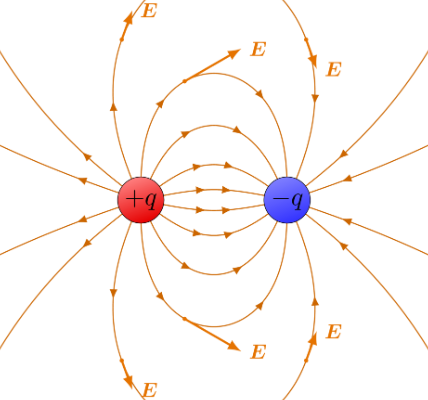
\includegraphics[scale = 0.4]{image/dipolo.png}
    \caption{campo elettromagnetico formato da un dipolo}
    \label{OndeElettrtomagnetiche}
\end{figure}

Se prendessimo un dipolo, insieme di cariche positive e negative bilanciate, e iniziassimo a muoverle esse genererebbero un campo elettrico variabile nel tempo. Dunque in ogni punto si genera un campo magnetico perpendicolare al campo elettrico. Nel caso della Figura \ref{OndeElettrtomagnetiche} ci potremmo immaginare un cerchio che esce dal foglio, e quello rappresenterebbe il campo magnetico, crea un vortice che attraversa il foglio. Questo procedimento si ripete all'infinito ed otteniamo le onde elettromagnetiche mostrate nella seguente Figura.

\begin{figure}[h]
    \centering
    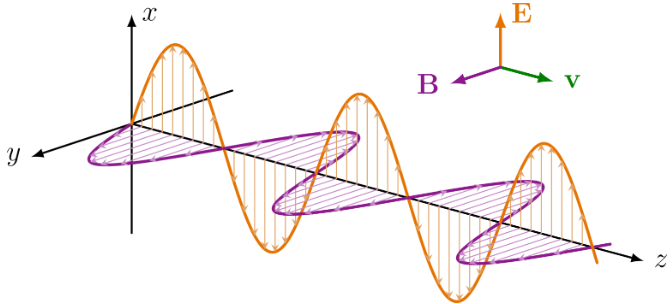
\includegraphics[scale=0.5]{image/ondeElettomagnetiche.png}
    \caption{Propagazione onde elettromagnetiche}
    \label{OndeElettromagentiche}
\end{figure}

Dal punto di vista delle equazioni non c'è un limite di frequenza delle oscillazioni ma tecnologicamente parlando si è arrivati all'ordine dei Gigahertz, un miliardo di oscillazioini al secondo.
\paragraph{}
Ora queste equazioni, per studiare le onde elettromagnetiche, si dovrebbero trasformare in equazioni differenziali perché così guardiamo cosa succede nel singolo punto e non cosa succede nell'insieme.

\section{Equazioni differenziali di Maxwell}

La trasformazione delle equazioni integrali in equazioni differenziali è possibile facendo tendere a zero il volume della superficie chiusa dove è applicato l'integrale.

\begin{equation*}
    \lim_{\Delta v \to 0}  \frac{\oint_s \vec{E} \cdot d\vec{s}}{\Delta v}  = \vec{\nabla}\cdot \vec{E}
\end{equation*}
questo limite ci da la divergenza, uno scalare il quale è la somma di tutte le componenti del gradiente, del campo elettrico. La divergenza di un campo vettoriale è la descrizione matematica
della tendenza del campo a “fuoriuscire” da un punto.

\paragraph{}
In modo analogo si trova l'equazione differenziale lungo una linea chiusa.

\begin{equation*}
    \lim_{\Delta s \to 0}  \frac{\oint_l \vec{E} \cdot d\vec{l}}{\Delta s}  = \vec{\nabla} \times \vec{E}
\end{equation*}

in questo altro caso il limite restituisce il rotore del campo elettrico. Il rotore di un campo vettoriale misura la tendenza del campo a “circolare” attorno a un punto.

\paragraph{}
Dunque le equazioni in forma differenziale diventano:

\begin{equation*}
    1)\vec{\nabla}\cdot \vec{E}  = \frac{\rho}{\varepsilon_0}\qquad3)\,\vec{\nabla} \cdot \vec{B}  = 0
\end{equation*}

\begin{equation*}
    2)\vec{\nabla} \times \vec{E}  = -\frac{d\vec{B}}{dt}\qquad4)\,\vec{\nabla} \times \vec{B}  = \mu_0 \vec{J} + \varepsilon_0\mu_0\frac{d\vec{E}}{dt}
\end{equation*}

\section{Formula di Biot-Savart o prima formula di Laplace}

Questa formula è la sorella della Formula di Coulomb, ma applicata al campo magnetico:

\begin{equation}
    \vec{B} = \frac{\mu_0}{4\pi} \frac{q\vec{v} \times \vec{Ur}}{r^2}
\end{equation}

In un dato punto: 

\begin{equation}
    d\vec{B} = \frac{\mu_0}{4\pi} \frac{i d\vec{l} \times \vec{Ur}}{r^2}
\end{equation}

\section{Filo infinito}

\begin{figure}[H]
    \centering
    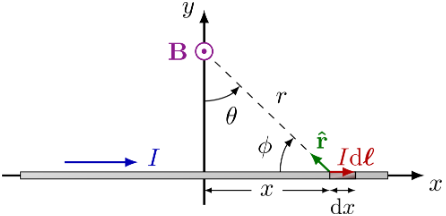
\includegraphics[scale = 0.5]{image/filoInfinitoMagnetico.png}
    \caption{Campo magnetico ad una distanza h dal filo}
    \label{campoMagneticodaUnFiloLeggeBiotSavart}
\end{figure}

\begin{equation}
    d\vec{B} = \frac{\mu_0}{4\pi} \frac{i d\vec{l} \times \vec{Ur}}{r^2}
\end{equation}

Per calcolarlo dobbiamo trasformare tutto in funzione di Theta. Quindi:

\begin{equation*}
    \frac{x}{r} = \tan{\theta}
\end{equation*}
\begin{equation*}
    x = r\tan{\theta}
\end{equation*}
\begin{equation*}
    dx = \frac{r}{\cos^2{\theta}} d\theta
\end{equation*}

\begin{equation*}
    \frac{d}{r} = \cos{\theta}
\end{equation*}
dove $d$ è la distanza dal filo.
\begin{equation*}
    r = \frac{d}{\cos{\theta}}
\end{equation*}

Quindi la formula risulta essere la seguente:

\begin{equation*}
    d\vec{B} = \frac{\mu_0}{4\pi} \frac{i d d\theta \cos{\theta}}{\cos^2{\theta}} \frac{\cos^2{\theta}}{d^2}
\end{equation*}

Semplificando e integrando:

\begin{equation}
    B = \frac{\mu_0 i}{4\pi d}\int_{-\theta} ^{\theta} \cos{\theta} d\theta
\end{equation}

dove $d$ è sempre la distanza tra il punto e il filo. Questo risultato lo avevamo già trovato servendoci della legge di Ampere, infatti se prendiamo $\theta = \frac{\pi}{2}$ avremo proprio:

\begin{equation}
    B = \frac{\mu_0 i}{2 \pi d}\
\end{equation}



Si preferisce usare questa formula perché la legge di Biot-Savart è valida su qualsiasi filo.


\section{Spira}

\begin{figure}[H]
    \centering
    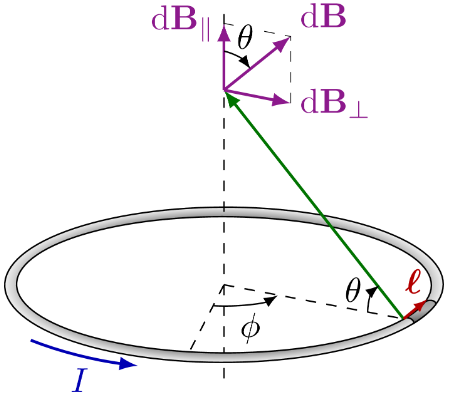
\includegraphics[scale = 0.5]{image/spira.png}
    \caption{Campo magnetico generato da una spira}
    \label{spira}
\end{figure}

\begin{equation}
    B = \frac{\mu_0 i r^2}{2(r^2 + h^2)^{\frac{3}{2}}}
\end{equation}

Dove $r$ risulta essere il raggio e $h$ l'altezza che vi è tra la spira e il punto.

\section{Applicazione della legge di Faraday}

\begin{figure}[H]
    \centering
    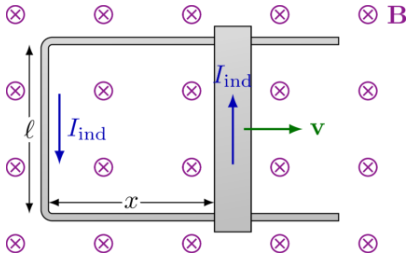
\includegraphics[scale = 0.5]{image/FaradayApplicazione.png}
    \caption{Induzione elettromagnetica}
    \label{FaradayApplicazione}
\end{figure}

Vorremmo calcolare il campo magnetico dell'area compresa tra il filo e la barra.

Per la legge di Faraday calcoliamo facilmente il flusso:

\begin{equation*}
    \oint_l \vec{E} \cdot d\vec{l}  = -\frac{d}{dt}\phi_b
\end{equation*}

dove $\phi_b = Blvt$ 

Derivandola nel tempo troviamo che:

\begin{equation}
    f.e.m.\footnote{f.e.m. = Forza ElettroMotrice, è una differenza di potenziale} = \oint_l \vec{E} \cdot d\vec{l}  = Blv
\end{equation}

L'area sta aumentando quindi il flusso di B sta aumentando, ed esso crea un campo elettrico e dunque una corrente. Tale corrente risulta essere:

\begin{equation*}
    I = \frac{f.e.m}{R}
\end{equation*}

Dove $R$ si intende la resistenza nel circuito.

Questo fenomeno si chiama \textbf{induzione elettromagnetica}.

\section{Legge di Lorentz}
Ogni carica sulla barretta viene spostata con una verta velocità $v$, quindi si genera una forza, concorde al segno della corrente e tale forza risulta essere:

\begin{equation}
    \vec{F} = qvB
\end{equation}

e dunque il lavoro di una forza risulta essere:

\begin{equation}
    L = qvBl
\end{equation}

e il lavoro per unità di carica è:
\begin{equation}
    \frac{L}{q} = Blv
\end{equation}

e risulta essere uguale proprio alla $f.e.m.$.

\section{Induttore}

\begin{figure}[H]
    \centering
    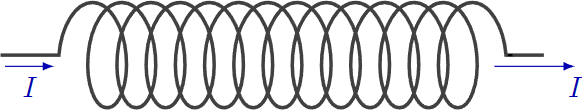
\includegraphics[scale = 0.4]{image/solenoide.png}
    \caption{Induttore}
    \label{Induttore}
\end{figure}

L'induttore è un componente elettrico che genera un campo magnetico al passaggio di corrente elettrica.

Formula principale:

\begin{equation}
    \Delta V = L \frac{dI}{dt}
\end{equation}

Ciò significa che la differenza di potenziale ai capi del solenoide risulta proporzionale ad $L$, l'induttanza, moltiplicato alla derivata nel tempo della corrente, una corrente variabile nel tempo.

Questa relazione può essere dedotta dalle equazioni di base dell'elettromagnetismo grazie alla legge di Ampere, e che abbiamo già dimostrato in precendenza:

\begin{equation}
    B = \frac{\mu_0IN}{l}
\end{equation}

dove $l$ è la lunghezza del solenoide considerato.


Se la corrente I che scorre nel solenoide/induttore è variabile nel tempo, anche B sarà variabile nel tempo. Essendo B variabile nel tempo, si produce una variazione di flusso del campo magnetico concatenato con il solenoide stesso il che produce, per la legge di Faraday, una f.e.m. auto-indotta ai capi dell'induttore, e dunque anche una differenza di potenziale tra una spira e l'altra.

\paragraph{}
Infatti per la legge di Faraday possiamo scrivere che su ogni spira si crea una differenza di potenziale:

\begin{equation*}
    -\frac{d \phi_B}{dt} = El = \Delta V
\end{equation*}
dove $l$ in questo caso è un giro della spira.

per trovare la differenza di potenziale totale, basta moltiplicarlo per il numero di spire $N$:

\begin{equation*}
    \Delta V_{tot} = N \frac{d \phi_B}{dt}
\end{equation*}
\begin{equation*}
    \Delta V_{tot} = N A \frac{\mu_0 N}{l} \frac{d I}{dt} 
\end{equation*}

dove $A$ risulta essere la sezione del tubo, $N$ il numero di spire e $l$ la lunghezza del solenoide.


$A \frac{\mu_0 N}{l}$, viene chiamata auto-induttanza o più semplicemente induttanza e si indica con L.

ecco dimostrato la legge di prima:

\begin{equation}
    \Delta V = \frac{d \phi_B}{dt} = L \frac{d I}{dt} 
    \label{eqSolenoide}
\end{equation}


Il solenoide è un parente stretto del condensatore, infatti oltre alla Equazioni \ref{equazioneCondensatore} e \ref{eqSolenoide}, che legano la corrente e la tensione, possiamo fare un discorso analogo che abbiamo già fatto per il condensatore: vogliamo capire dove va a finire l'energia elettrica che abbiamo usato per caricare l'induttore? Per carica di un induttore significa che si fa passare una corrente ai suoi capi e quando risulta costante allora al suo interno si è creato un campo magnetico costante.

\paragraph{}
Bene questa energia è stipata all'interno del area del solenoide. E da notare che in questo caso non si parla più di energia potenziale, come nel condensatore, ma bensì si parla di energia cinetica. 

\section{Circuito LC}

\begin{figure}[H]
    \centering
    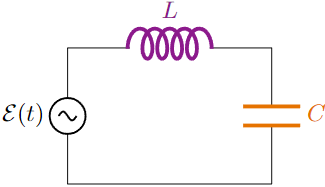
\includegraphics[scale = 0.6]{image/circuito_LC.png}
    \caption{Circuito LC}
    \label{ciruitoLc}
\end{figure}

Se creiamo un circuito formato da un induttore e da una condensatore carico otterremo un circuito risonante, perché il condensatore trasferirà tutta la sua energia, scaricandosi, all'induttore il quale si caricherà e una volta carico inizierà a ridare energia al condensatore e il ciclo riparte. Quindi questo circuito si comporta esattamente come un pendolo.
\paragraph{}
Quindi questo modo permette di creare dei clock, dei timer; ovviamente la corrente si consumerebbe nel tempo, come nel caso del pendolo, infatti si deve mantenere una tensione costante, infatti bisogna inserire anche un generatore il quale vada alla stessa frequenza con cui il circuito oscilla.

\paragraph{}
L'equazione del risonatore è:

\begin{equation}
    LC + \frac{d^2I}{dt^2} + I = 0
\end{equation}

Il risultato di questa equazione differenziale, dopo aver applicato le regole di risoluzione delle equazioni differenziali troviamo il seguente risultato:

\begin{equation}
    I(t) = I_0 \cos{\omega t}\qquad\omega = \frac{1}{\sqrt{LC}}
\end{equation}

Ovvero una corrente oscillante nel tempo.


\afterpage{\blankpage}
\afterpage{\blankpage}

\begin{thebibliography}{9}

\bibitem{Tikz}
Tutti i grafici ed alcune immagini presenti in questo manuale sono state prese e modificate dal sito: \href{https://tikz.net/}{tikz.net}.

\bibitem{Contenuti}
I contenuti di questo manuale fanno fedelmente riferimento agli argomenti spiegati nel corso di Fisica I tenuto dal Professore Zeno Gaburro, e presenti sulla piattaforma del corso: \href{https://class.kadidak.com/}{class.kadidak.com}.

\bibitem{YouMath, Wikipedia, Edutecnica}
Molte parti sono state integrate con esempi e spiegazioni presi dai siti: \href{https://www.youmath.it/}{youmath.it}, \href{https://it.wikipedia.org/}{it.wikipedia.org}, \href{https://www.edutecnica.it/}{edutecnica.it}.


\begin{figure}[b]
    \centering
    
\includegraphics[scale = 0.5]{image/by-sa.png}
    \captionsetup{labelformat=empty}
    \captionsetup{justification=centering}
    \caption{Licensed under a Creative Commons Attribution-ShareAlike 4.0 International License with \textcopyright \, Copyright 2023 – Cristiano Berardo.}
\end{figure}

\end{thebibliography}

\afterpage{\blankpage}
\end{document}
